%\input{/Volumes/SOURCE/Cours/Mathematiques/Preambule/preambule-sacha-utf8.ltx}
\input{./preambule-sacha-utf8.ltx}
   	 
	
% \usepackage[utf8x]{inputenc} 
\usepackage[T1]{fontenc} 
\usepackage[a4paper,left=2cm,right=2cm,top=2cm,bottom=2cm]{geometry} 
\usepackage{lmodern} 
\usepackage{graphicx} 
% \usepackage[french]{babel} 
\usepackage{fancyhdr}

\usepackage{textcomp}
\usepackage{texgraph}
\usepackage{pgf,tikz}
\usetikzlibrary{arrows}

\usepackage{variations}


\ifdefined\COMPLETE
\else
    \newcommand{\COMPLETE}
\fi                        % Autorise la compilation de illustrations
                          % soit isolées, soit inluses 
                          
%\iffalse

\title {  \Huge     Mathématiques\\
             Première économique et sociale \\
       }

\author{ \Large   Monsieur Hilaire  }

\date  { \large  Année 2013-2014   }

%\fi

\begin{document}

%\iffalse

\maketitle\thispagestyle{empty} % Cette forme est obligatoire, sinon numero
\vfill

\centerline {\large  Lycée International de Saint-Germain-en-Laye} 

\newpage

\thispagestyle{empty}

\def\TikZ{{\fontfamily{cmr}Ti{\em k}Z}} 
    \begin {quote}
    Ce document a été composé sous  Unix\footnote{Unix  est une
    marque déposée des  Laboratoires  Bell d'{\sc att}} au moyen  
    du logiciel \LaTeX (domaine  public),
    et de l'éditeur {\TeX}{Maker}\footnote{TeXmaker (créé par Pascal Brachet en 2003) est un éditeur libre de documents LaTeX, utilisable sur Linux, Mac et Windows.} (domain public). 
    Les figures ont été réalisées avec {\TikZ}\footnote{TikZ est une extension permettant de générer des images PGF. Selon son auteur Till Tantau, TikZ est un acronyme récursif qui veut dire « TikZ ist kein Zeichenprogramm » : TikZ n'est pas un logiciel de dessin - au sens de « TikZ est un langage pour graphiques ».} (domaine
   public)  et  intégrées  directement  dans le  document  final. \\
   
   Ce document n'aurait pu être réalisé sans l'étroite collaboration de Valérie Panyusko, Liliana Rodrigues Brites et Joseph de Larauze. Je les remercie infiniment pour leur aide précieuse dans la création de ce deuxième tome des cours de Pierre-Étienne Hilaire. \\
   
   Les sujets des devoirs sont donnés en annexes, nouveauté pour ce deuxième tome. Les barèmes sont donnés à titre indicatif. \\
   
    \end {quote}

   \vspace {12cm}
% \centerline {\large \textcopyleft Lycée International de Saint-Germain-en-Laye} 

   \begin {quote}
   \em Les enseignants et formateurs demeurent titulaires des droits d'auteur sur les cours qu'ils dispensent.    
Dans la mesure où l'auteur n'a pas renoncé à ses droits, les modifications de sa création, qui constituent une œuvre dérivée, nécessitent son autorisation. 
    Toute  reproduction,  sans le consentement de l'auteur, 
    même  partielle,  de ce document est
    interdite.  Une copie ou reproduction  par quelque procédé que
    ce   soit,   photographie,    photocopie,   microfilm,   bande
    magnétique,   disque  ou  autre,   constitue  une  contrefaçon
   passible  de la loi du 11  mars  1957  sur la  protection  des
    droits d'auteur.
    \end {quote}
\newpage

\setcounter{page}{1}

% Début de la table des matières. Le groupe dedans permet de régler la taille, de telle sorte que les paragraphes ne soient pas coupés en plein milieu.

\begingroup
\baselineskip\dimexpr\baselineskip-.9pt\relax
\tableofcontents
\endgroup

% Fin de la table des matières.

\newpage
~ % On veut commencer sur une page de droite 
\newpage

%\fi

\ifdefined\COMPLETE
\else
    \input{./preambule-sacha-utf8.ltx}
    \begin{document}
\fi


\vspace*{-1.5cm}

\part{Les trinômes du second degré}

\section{Introduction}

\subsection{Rappel des années antérieures}

Résoudre les équations suivantes dans $\R$ :

\subsubsection{Exemple \no 1}

$x^2 - 9 = 0$ \\

Il faut factoriser. \\

\textbf{Rappel :} En troisième, on a appris trois identités remarquables : \\

\begin{itemize}
\item[•] $\left(a + b \right)^2 = a^2 + 2ab + b^2$ 
\item[•] $\left(a - b \right)^2 = a^2 - 2ab + b^2$ 
\item[•] $a^2 - b^2 = \left(a+b\right)\left(a-b\right)$ 
\end{itemize}

\vspace*{.3cm}

On a donc $x^2 - 9 = 0 \Longleftrightarrow \left(x+3\right)\left(x-3\right) = 0$. \\

\textbf{Rappel :} En troisième, on a appris si un produit est nul, au moins l'un de ses facteurs est nul. \\

\begin{tabular}{lll}
D'où $\left(x+3\right)\left(x-3\right) = 0$ & $ \Longleftrightarrow $ & $  x+3 = 0 $ ou $ x-3 = 0$ \\
& $\Longleftrightarrow$ & $x = -3 $ ou $x=3$ \\
\end{tabular}

Ainsi, $S = \lb -3 \; ; \; 3 \; \rb $

\subsubsection{Exemple \no 2}

\begin{tabular}{lll}
$ 9x^2 - 5 = 0$ & $\Longleftrightarrow$ & $\left(3x + \sqrt{5}\right)\left(3x - \sqrt{5}\right) = 0$ \\
& $\Longleftrightarrow$ & $3x + \sqrt{5} = 0 $ ou $3x - \sqrt{5} = 0$ \\
& $\Longleftrightarrow$ & $3x = -\sqrt{5}$ ou $3x = \sqrt{5}$ \\
& $\Longleftrightarrow$ & $x = \dfrac{-\sqrt{5}}{3} $ ou $x = \dfrac{\sqrt{5}}{3} $ \\
\end{tabular}

\vspace*{.3cm}

D'où $ S = \lb \dfrac{-\sqrt{5}}{3} \; ; \; \dfrac{\sqrt{5}}{3} \rb $

\subsubsection{Exemple \no 3}

\begin{tabular}{lll}
$x^2 - 14x + 49 = 0$ & $\Longleftrightarrow$ & $\left(x-7\right)^2 = 0 $\\
& $\Longleftrightarrow$ & $\left(x-7\right)\left(x-7\right) = 0$ \\
& $\Longleftrightarrow$ & $x-7 = 0$ ou $x-7 = 0$ \\
& $\Longleftrightarrow$ & $x = 7$ ou $x = 7$ \\
\end{tabular}

\vspace*{.3cm}

D'où $S = \lb 7 \rb $. \\

\textbf{N.B. :} Cet ensemble de solution est un \textbf{singleton}, bien que l'équation soit une équation du second degré. Cette solution est en fait une \textbf{solution double}.

\subsubsection{Exemple \no 4}

\begin{tabular}{lll}
$3x^2 - 2x\sqrt{21} + 7 = 0$ & $\Longleftrightarrow$ & $\left(x\sqrt{3} - \sqrt{7}\right)^2 = 0 $ \\
& $\Longleftrightarrow$ & $x\sqrt{3} - \sqrt{7} = 0$ \\
& $\Longleftrightarrow$ & $x\sqrt{3} = \sqrt{7}$ \\
& $\Longleftrightarrow$ & $ x = \dfrac{\sqrt{7}}{\sqrt{3}}$ \\
& $\Longleftrightarrow$ & $x = \dfrac{\sqrt{21}}{3}$ \\
\end{tabular}

D'où $ S = \lb \dfrac{\sqrt{21}}{3} \rb $

\subsubsection{Exemple \no 5}

\begin{tabular}{lll}
$x^2 + 36 = 0$ & $\Longleftrightarrow$ & $x^2 = -36$ \\
\end{tabular}

\vspace*{.3cm} 

Or, $\forall x \in \R, x^2 \geqslant 0$. \\

D'où $ S = \varnothing$ 

\subsubsection{Exemple \no 6}

\begin{tabular}{lll}
$17x^2 + 13 = 0 $ & $\Longleftrightarrow$ & $ 17x^2 = -13$ \\
\end{tabular}

\vspace*{.3cm}

Or, $\forall x \in \R, \forall a \in \R^+, ax^2 \geqslant 0$. \\

D'où $ S = \varnothing $

\subsection{Factoriser grâce à un « morceau » d'identité remarquable}

\subsubsection{Exemple \no 1}

\begin{tabular}{lll}
$x^2 + 6x - 7 = 0$ & $\Longleftrightarrow$ & $\left(x^2 + 6x + 9\right) - 16 = 0 $ \\
& $\Longleftrightarrow$ & $\left(x + 3\right)^2 - 4^2 = 0$ \\
& $\Longleftrightarrow$ & $\left(x + 3 + 4\right)\left(x + 3 - 4 \right) = 0 $ \\
& $\Longleftrightarrow$ & $\left(x + 7\right)\left(x - 1\right) = 0 $ \\
& $\Longleftrightarrow$ & $x + 7 = 0 $ ou $x - 1 = 0$ \\
& $\Longleftrightarrow$ & $ x = -7 $ ou $x = 1$ \\
\end{tabular}

\vspace*{.3cm}

D'où $S = \lb -7 \; ; \; 1 \rb$ 

\subsubsection{Exemple \no 2}

\begin{tabular}{lll}
$x^2 - 14x - 34 = 0 $ & $\Longleftrightarrow$ & $\left(x^2 - 14x + 49\right) - 81 = 0$ \\
& $\Longleftrightarrow$ & $\left(x-7\right)^2 - 9^2 = 0 $ \\
& $\Longleftrightarrow$ & $\left(x-7 + 9\right)\left(x-7 - 9\right) = 0$ \\
& $\Longleftrightarrow$ & $\left(x + 2\right)\left(x - 16\right) = 0$ \\
& $\Longleftrightarrow$ & $x + 2 = 0$ ou $x - 16 = 0$ \\
& $\Longleftrightarrow$ & $x = -2$ ou $x = 16$ \\
\end{tabular}

\vspace*{.3cm}

D'où $S = \lb -2 \; ; \; 16 \rb $ 

\subsubsection{Exemple \no 3}

\begin{tabular}{lll}
$x^2 - 5x + 4 = 0$ & $\Longleftrightarrow$ & $\left(x^2 - 5x + \dfrac{25}{4} \right) - \dfrac{9}{4} = 0$ \\
& $\Longleftrightarrow$ & $\left(x - \dfrac{5}{2}\right)^2 - \left(\dfrac{3}{2}\right)^2 = 0$ \\
& $\Longleftrightarrow$ & $\left(x - \dfrac{5}{2} + \dfrac{3}{2}\right)\left(x - \dfrac{5}{2} - \dfrac{3}{2} \right) = 0$ \\
& $\Longleftrightarrow$ & $\left(x-1\right)\left(x-4\right) = 0$ \\
& $\Longleftrightarrow$ & $ x -1 = 0$ ou $x - 4 = 0$ \\
& $\Longleftrightarrow$ & $ x = 1 $ ou $ x = 4 $ \\
\end{tabular}

\vspace*{.3cm}

D'où $S = \lb 1 \; ; \; 4 \rb $ 

\subsubsection{Exemple \no 4}

\begin{tabular}{lll}
$x^2 + 15x - 76 = 0 $ & $\Longleftrightarrow$ & $\left(x^2 + 15x + \dfrac{225}{4}\right) - \dfrac{529}{4} = 0$ \\
& $\Longleftrightarrow$ & $\left(x + \dfrac{15}{2}\right)^2 -  \left(\dfrac{23}{2}\right)^2 = 0$ \\
& $\Longleftrightarrow$ & $\left(x + \dfrac{15}{2} + \dfrac{23}{2}\right)\left(x + \dfrac{15}{2} - \dfrac{23}{2}\right) = 0$ \\
& $\Longleftrightarrow$ & $\left(x + 19\right)\left(x - 4\right) = 0$ \\
& $\Longleftrightarrow$ & $x + 19 = 0 $ ou $x - 4 = 0$ \\
& $\Longleftrightarrow$ & $x = -19 $ ou $x = 4$ \\
\end{tabular}

D'où $S = \lb -19 \; ; \; 4 \rb $ 

\subsubsection{Exemple \no 5}

\begin{tabular}{lll}
$9x^2 - 30x + 9 = 0$ & $\Longleftrightarrow$ & $\left(9x^2 - 30x +25\right) - 16 = 0 $ \\
& $\Longleftrightarrow$ & $\left(3x - 5\right)^2 - 4^2 = 0$ \\
& $\Longleftrightarrow$ & $\left(3x -5 + 4\right)\left(3x - 5 - 4\right) = 0$ \\
& $\Longleftrightarrow$ & $\left(3x -1\right)\left(3x - 9\right) = 0$ \\
& $\Longleftrightarrow$ & $ 3x - 1 = 0 $ ou $3x - 9 = 0$ \\
& $\Longleftrightarrow$ & $3x = 1 $ ou $3x = 9$ \\
& $ \Longleftrightarrow$ & $ x = \dfrac{1}{3} $ ou $x = 3$ \\
\end{tabular}

\vspace*{.3cm}

D'où $S = \lb \dfrac{1}{3} \; ; \; 3 \rb $ 

\subsubsection{Exemple \no 6}

\begin{tabular}{lll}
$36x^2 + 84x - 95 = 0 $ & $\Longleftrightarrow$ & $\left(36x^2 + 84x + 49\right) - 144 = 0 $ \\
& $\Longleftrightarrow$ & $\left(6x + 7\right)^2 - 12^2 = 0$ \\
& $\Longleftrightarrow$ & $\left(6x + 7 + 12\right)\left(6x + 7 - 12\right) = 0$ \\
& $\Longleftrightarrow$ & $\left(6x + 19\right)\left(6x -5\right) = 0$ \\
& $\Longleftrightarrow$ & $6x + 19 = 0$ ou $6x - 5 = 0$ \\
& $\Longleftrightarrow$ & $6x = -19$ ou $6x = 5$ \\
& $ \Longleftrightarrow$ & $x = \dfrac{-19}{6}$ ou $x = \dfrac{5}{6}$ \\
\end{tabular}

\vspace*{.3cm}

D'où $S = \lb \dfrac{-19}{6} \; ; \; \dfrac{5}{6} \rb $ 

\subsubsection{Exemple \no 7}

\begin{tabular}{lll}
$x^2 - 14x + 74 = 0$ & $\Longleftrightarrow$ & $\left(x^2 - 14x + 49\right) + 25 = 0$ \\
& $\Longleftrightarrow$ & $\left(x-7\right)^2 + 5^2 + 0$ \\
& $\Longleftrightarrow$ & $\left(x-7\right)^2 = -5^2 $ \\
\end{tabular}

Or $\forall x \in \R, x^2 \geqslant 0$. \\

D'où $S = \varnothing$ \\

\subsubsection{Exemple \no 8}

\begin{tabular}{lll}
$25x^2 + 20x + 53 = 0$ & $\Longleftrightarrow$ & $\left(25x^2 + 20x + 4\right) + 49 = 0$ \\
& $\Longleftrightarrow$ &  $\left(5x + 2\right)2 + 7^2 = 0$ \\
& $\Longleftrightarrow$ & $\left(5x + 2\right)^2 = -7^2$ \\
\end{tabular}

Or $\forall x \in \R, x^2 \geqslant 0$. \\

D'où $S = \varnothing$ 

\newpage

\section{Formules fondamentales}

\subsection{Résolutions, dans $\mathbf{\R}$, dans tous les types d'équations du second degré }

On peut écrire, pour $a$, $b$ et $c$ trois nombres réels avec $a \neq 0$, toutes les équations du second degré sous la forme : $ax^2 + bx + c = 0$. \\

\begin{tabular}{lll}
$ax^2 + bx + c = 0$ & $\Longleftrightarrow$ & $a\left(x^2 + \dfrac{b}{a}x + \dfrac{c}{a}\right) = 0$ \\
& $\Longleftrightarrow$ & $x^2 + \dfrac{b}{a}x + \dfrac{c}{a} = 0$ \\
& $\Longleftrightarrow$ & $ \left(x^2 + \dfrac{b}{a} x + \dfrac{b}{4a^2}\right) - \dfrac{b^2 - 4ac}{4a^2} = 0 $ \\
& $\Longleftrightarrow$ & $\left(x + \dfrac{b}{2a} \right)^2 - \dfrac{b^2 - 4ac}{\left(2a\right)^2} = 0$. \\
\end{tabular}

\vspace*{.3cm}

On a $\left(x + \dfrac{b}{2a}\right)^2 \geqslant 0$ et $\left(2a\right)^2 \geqslant 0$. \\

Notons alors $ \Delta = b^2 - 4ac$. \\

On a : $\left(x + \dfrac{b}{2a} \right)^2 - \dfrac{\Delta}{\left(2a\right)^2} = 0$ 

\begin{itemize}
\item[•] 1$^\mathrm{er}$ cas : $\Delta > 0$. \\

Si $\Delta > 0$, alors $\dfrac{\Delta}{\left(2a\right)^2} = \left(\dfrac{\sqrt{\Delta}}{2a}\right)^2$ \\


\begin{tabular}{lll}
Ainsi, on a : $\left(x + \dfrac{b}{2a} \right)^2 - \dfrac{\Delta}{\left(2a\right)^2} = 0$ & $\Longleftrightarrow$ & $\left(x + \dfrac{b}{2a} \right)^2 - \left(\dfrac{\sqrt{\Delta}}{2a}\right)^2 = 0 $ \\
& $\Longleftrightarrow$ & $\left(x + \dfrac{b}{2a} + \dfrac{\sqrt{\Delta}}{2a}\right)\left(x + \dfrac{b}{2a} - \dfrac{\sqrt{\Delta}}{2a}\right) = 0$ \\
& $\Longleftrightarrow$ & $ x + \dfrac{b + \sqrt{\Delta}}{2a} = 0 $ ou $x + \dfrac{b - \sqrt{\Delta}}{2a} = 0 $ \\
& $\Longleftrightarrow$ & $ x = -\dfrac{b + \sqrt{\Delta}}{2a}$ ou $x = \dfrac{b - \sqrt{\Delta}}{2a}$ \\
& $\Longleftrightarrow$ & $ x = \dfrac{-b - \sqrt{\Delta}}{2a}$ ou $x = \dfrac{-b + \sqrt{\Delta}}{2a}$ \\
\end{tabular}

\vspace*{.3cm}

D'où $ S = \lb \dfrac{-b - \sqrt{\Delta}}{2a} \; ; \; \dfrac{-b + \sqrt{\Delta}}{2a} \rb $. \\ 

On dit que le trinôme à \textbf{2 racines}. \\

\newpage

\item[•] 2$^\mathrm{ème}$ cas : $\Delta = 0$ \\

Si $\Delta = 0$, alors $\dfrac{\Delta}{\left(2a\right)^2} = 0$ \\

\begin{tabular}{lll}
Ainsi, on a : $\left(x + \dfrac{b}{2a} \right)^2 - \dfrac{\Delta}{\left(2a\right)^2} = 0$ & $\Longleftrightarrow$ & $\left(x + \dfrac{b}{2a} \right)^2  0$ \\
& $\Longleftrightarrow$ & $x + \dfrac{b}{2a} = 0$ \\
& $\Longleftrightarrow$ & $x = -\dfrac{b}{2a}$ \\
\end{tabular}

\vspace*{.3cm}

D'où $ S = \lb -\dfrac{b}{2a} \rb $. \\ 

On dit que le trinôme à une \textbf{racine double}. \\

\item[•]3$^\mathrm{ème}$ cas : $\Delta < 0$ \\

\begin{tabular}{lll}
Ainsi, on a : $\left(x + \dfrac{b}{2a} \right)^2 - \left(  \dfrac{\Delta}{\left(2a\right)^2}\right) = 0$ & $\Longleftrightarrow$ & $\left(x + \dfrac{b}{2a}\right)^2 = \dfrac{\Delta}{\left(2a\right)^2}$ \\
\end{tabular}

\vspace*{.3cm}

Or, $\Delta < 0$, donc $\dfrac{\Delta}{\left(2a\right)^2} < 0$. \\

Cependant, $\forall x \in \R, x^2 \geqslant 0$. \\

Ainsi, l'équation $\left(x + \dfrac{b}{2a}\right)^2 = \dfrac{\Delta}{\left(2a\right)^2}$ n'a pas de solution. \\

D'où $S = \varnothing$
\end{itemize}

\vspace*{.3cm}

\textbf{Récapitulatif} \\

$\forall a \in \R^*, \forall b \in \R, \forall c \in \R, ax^2 + bx + c = 0$ est un trinôme du second degré. \\

Soit $\Delta = b^2 - 4ac$ le discriminant de l'équation. \\

\begin{tabular}{lll}
Si $\Delta > 0$, alors le trinôme a deux racines, et $S = \lb \dfrac{-b - \sqrt{\Delta}}{2a} \; ; \; \dfrac{-b + \sqrt{\Delta}}{2a} \rb $ \\
Si $\Delta = 0$, alors le trinôme a une racine double, et $S = \lb -\dfrac{b}{2a} \rb $ \\
Si $\Delta < 0$, alors le trinôme n'a pas de racine réelle, et $ S = \varnothing$ \\
\end{tabular}

\newpage

\subsection{Exercices}

\subsubsection{Exemple \no 1}

$x^2 - 14x - 32 = 0$ \\

On a $a = 1$, $b = -14$, $c = -32$. \\

$ \Delta = b^2 - 4ac = 196 - 4 \times \left(-32\right) = 196 + 128 = 324 = 18^2$. \\

$\Delta > 0$, donc l'équation a deux solutions : \\

\begin{tabular}{lll}
$x_1 = \dfrac{-b - \sqrt{\Delta}}{2a}$ & ou & $x_2 = \dfrac{-b + \sqrt{\Delta}}{2a}$ \vspace*{.3cm} \\
$ x_1 = \dfrac{14 - 18}{2}$ & ou &$x_2 = \dfrac{14 + 18}{2}$ \vspace*{.3cm} \\
$x_1 = \dfrac{-4}{2}$ & ou & $x_2 = \dfrac{32}{2}$ \vspace*{.3cm} \\
$x_1 = -2$ & ou &$x_2 = 16$ \\
\end{tabular}

\vspace*{.3cm}

D'où $S = \lb -2 \; ; \; 16 \rb$. 

\subsubsection{Exemple \no 2}

$x^2 + 15x - 76 = 0$ \\

On a $a = 1$, $b = 15$, $c = -76$. \\

$ \Delta = b^2 - 4ac = 225 - 4 \times \left(-76\right) = 225 + 304 = 529 = 23^2$. \\

$\Delta > 0$, donc l'équation a deux solutions : \\

\begin{tabular}{lll}
$x_1 = \dfrac{-b - \sqrt{\Delta}}{2a}$ & ou & $x_2 = \dfrac{-b + \sqrt{\Delta}}{2a}$ \vspace*{.3cm} \\
$ x_1 = \dfrac{-15 - 23}{2}$ & ou &$x_2 = \dfrac{-15 + 23}{2}$ \vspace*{.3cm} \\
$x_1 = \dfrac{-38}{2}$ & ou & $x_2 = \dfrac{8}{2}$ \vspace*{.3cm} \\
$x_1 = -19$ & ou &$x_2 = 4$ \\
\end{tabular}

\vspace*{.3cm}

D'où $S = \lb -19 \; ; \; 4 \rb$. 

\newpage

\subsubsection{Exemple \no 3}

$36x^2 + 84x - 95 = 0$ \\

On a $a = 36$, $b = 84$ et $c = -95$. \\

$\Delta = b^2 - 4ac = 7056 - 4\left(36 \times \left(-95\right)\right) = 7056 + 13680 = 20 736 = 144^2$. \\

$\Delta > 0$, donc l'équation a deux solutions : \\

\begin{tabular}{lll}
$x_1 = \dfrac{-b - \sqrt{\Delta}}{2a}$ & ou & $x_2 = \dfrac{-b + \sqrt{\Delta}}{2a}$ \vspace*{.3cm} \\
$x_1 = \dfrac{-84 - 144}{72}$ & ou & $x_2 = \dfrac{-84 + 144}{72}$ \vspace*{.3cm} \\
$x_1 = \dfrac{-228}{72}$ & ou & $x_2 = \dfrac{60}{72}$ \vspace*{.3cm} \\
$x_1 = \dfrac{-19}{6}$ & ou & $x_2 = \dfrac{5}{6}$ \\
\end{tabular}

D'où $S = \lb -\dfrac{19}{6} \; ; \; \dfrac{5}{6} \rb $ 

\subsubsection{Exemple \no 4}

$25x^2 + 20x + 53$ \\

On a $a = 25$, $b = 20$, $c = 53$ \\

$ \Delta = b^2 - 4ac = 400 - 4 \times 25 \times 53 = 400 - 5 300 = -4 900$ \\

$\Delta < 0$, donc l'équation n'a pas de solution. \\

D'où $S = \varnothing$. 

\subsubsection{Exemple \no 5}

$127x^2 - 5x - 23 = 0$ \\

On a $a = 127$, $b = -5$, $c = -23$. \\

$ \Delta = b^2 - 4ac = 25 - 4 \times 127 \times \left(-23\right) = 25 + 11684 = 11 709$ \\

$\Delta > 0$, donc l'équation a deux solutions : 

\begin{tabular}{lll}
$x_1 = \dfrac{-b - \sqrt{\Delta}}{2a}$ & ou & $x_2 = \dfrac{-b + \sqrt{\Delta}}{2a}$ \vspace*{.3cm} \\
$ x_1 = \dfrac{5 - \sqrt{11709}}{254}$ & ou &$x_2 = \dfrac{5 + \sqrt{11709}}{254}$ \vspace*{.3cm} \\
\end{tabular}

D'où $S = \lb \dfrac{5 - \sqrt{11 709}}{254} \; ; \; \dfrac{5 + \sqrt{11 709}}{254} \rb$ 

\subsubsection{Exemple \no 6}

$1369x^2 - 4514x + 3721 = 0 $ \\

On a $a = 1 369$, $b = -4 514$, et $c = 3 721$. \\

$ \Delta = b^2 - 4ac = 20 376 196 - 20 376 196 = 0$ \\

$\Delta = 0$, donc l'équation a une solution : \\

$ x = -\dfrac{b}{2a} = \dfrac{4 514}{2 738} = \dfrac{61}{37}$. \\

$ S = \lb \dfrac{61}{37} \rb $ 

\subsubsection{Exemple \no 7}

$37 412x^2 -x + 29 = 0$ \\

On a $ a = 37 412$, $b = -1$ et $c = 29$. \\

$\Delta = b^2 - 4ac = 1 - 4 \times 29 \times 4 339 792 < 0$ \\

$\Delta < 0$, donc l'équation n'a pas de solution. \\

$S = \varnothing$ 

\newpage

\section{Forme canonique du trinôme}

\subsection{Rappels}

\begin{tabular}{lllll}
Soit une fonction $f$ : & $\R$ & $\longrightarrow$ & $\R$ & \\
& $x$ & $\longrightarrow$ & $f\left(x\right) = ax^2 + bx + c$, & avec $a \neq 0$ \\ 
\end{tabular}

On rappelle que $f\left(x\right)$ est un nombre réel, et que $f\left(x\right) = 0$ est l'\textbf{équation associée} à la fonction $f$. \\ De plus, la fonction $f$ est une \textbf{fonction polynôme du second degré}, ou une \textbf{fonction trinôme}. \\

\textbf{Exemple} \\

\begin{tabular}{llll}
Soit une fonction $f$ : & $\R$ & $\longrightarrow$ & $\R$ \\
& $x$ & $\longrightarrow$ & $f\left(x\right) = x^2 - 2x - 3$ \\ 
\end{tabular}

\vspace*{.3cm}

\begin{tikzpicture}[line cap=round,line join=round,>=triangle 45,x=1.0cm,y=1.0cm, scale=0.75]
\draw[->,color=black] (-6.27,0) -- (9.19,0);
\foreach \x in {-6,-5,-4,-3,-2,-1,1,2,3,4,5,6,7,8,9}
\draw[shift={(\x,0)},color=black] (0pt,2pt) -- (0pt,-2pt) node[below] {\footnotesize $\x$};
\draw[->,color=black] (0,-4.58) -- (0,7.98);
\foreach \y in {-4,-3,-2,-1,1,2,3,4,5,6,7}
\draw[shift={(0,\y)},color=black] (2pt,0pt) -- (-2pt,0pt) node[left] {\footnotesize $\y$};
\draw[color=black] (0pt,-10pt) node[right] {\footnotesize $0$};
\clip(-6.27,-4.58) rectangle (9.19,7.98);
\draw  plot (\x,{(\x)*(\x)-2*\x-3});
\begin{pgfonlayer}{background}   
\draw[step=1mm,ultra thin,AntiqueWhite!10] (-6.27,-4.58) grid (9.19,7.98);
\draw[step=5mm,very thin,AntiqueWhite!30]  (-6.27,-4.58) grid (9.19,7.98);
\draw[step=1cm,very thin,AntiqueWhite!50]  (-6.27,-4.58) grid (9.19,7.98);
\draw[step=5cm,thin,AntiqueWhite]          (-6.27,-4.58) grid (9.19,7.98);
\end{pgfonlayer} 
\end{tikzpicture}

\vspace*{.3cm}

Résolvons l'équation associée à la fonction $f$ :

\begin{tabular}{lll}
$\forall x \in \R, f\left(x\right) = 0$ & $\Longleftrightarrow$ & $x^2 - 2x - 3 = 0$ \vspace*{.3cm} \\
\end{tabular}

$\Delta = b^2 - 4ac = 4 - 4 \times \left(-3\right) = 4 + 12 = 16 = 4^2$ \\

$\Delta > 0$, donc l'équation a deux solutions : 

\begin{tabular}{lll}
$x_1 = \dfrac{-b - \sqrt{\Delta}}{2a}$ & ou & $x_2 = \dfrac{-b + \sqrt{\Delta}}{2a}$ \vspace*{.3cm} \\

$x_1 = \dfrac{2 - 4}{2}$ & ou & $x_2 = \dfrac{2 + 4}{2}$ \vspace*{.3cm} \\

$ x_1 = -1 $ & ou & $x_2 = 3$ \vspace*{.3cm} \\
\end{tabular} 

D'où $S = \lb -1 \; ; \; 3 \rb$. \\

Les solutions sont les abscisses des points d'intersection de la parabole et de l'axe des abscisses.

\newpage

\subsection{Généralisation de la factorisation des trinômes}

\begin{tabular}{lllll}
Soit une fonction $f$ : & $\R$ & $\longrightarrow$ & $\R$ & \\
& $x$ & $\longrightarrow$ & $f\left(x\right) = ax^2 + bx + c$, & avec $a \neq 0$ \\ 
\end{tabular}

\vspace*{.3cm}

Soient $\Delta$ le discriminant du trinôme, et $x_1$, $x_2$ ou $x_0$ ses racines éventuelles. \\

\begin{itemize}
\item[•] 1$^\mathrm{er}$ cas : $\Delta > 0$. \\

On a $ x_1 = \dfrac{-b - \sqrt{\Delta}}{2a}$ et $ x_2 = \dfrac{-b + \sqrt{\Delta}}{2a}$ \\

\begin{tabular}{lll}
$f\left(x\right)$ & $=$ & $ax^2 + bx + c$ \\
& $=$ & $a \left[\left(x + \dfrac{b}{2a}\right)^2 - \left(\dfrac{\sqrt{\Delta}}{2a}\right)^2 \right]$ \\
& $=$ & $a\left(x + \dfrac{b}{2a} + \dfrac{\sqrt{\Delta}}{2a} \right) \left(x + \dfrac{b}{2a} - \dfrac{\sqrt{\Delta}}{2a}\right)$ \\
& $=$ & $a\left(x + \dfrac{b + \sqrt{\Delta}}{2a} \right)\left(x + \dfrac{b - \sqrt{\Delta}}{2a} \right)$ \\
& $=$ & $a\left(x - \dfrac{-\left(b + \sqrt{\Delta}\right)}{2a} \right)\left(x - \dfrac{-\left(b - \sqrt{\Delta}\right)}{2a} \right)$ \\
& $=$ & $a\left(x - \dfrac{-b - \sqrt{\Delta}}{2a}\right)\left(x - \dfrac{-b + \sqrt{\Delta}}{2a}\right)$ \\
& $=$ & $a \left(x - x_1\right)\left(x - x_2\right)$ \\
\end{tabular}

\vspace*{.3cm}

\item[•]2$^\mathrm{ème}$ cas : $\Delta = 0$ \\

On a $x_0 = \dfrac{-b}{2a}$ \\

\begin{tabular}{lll}
$f\left(x\right)$ & $=$ & $ax^2 + bx + c$ \\
& $=$ & $a\left(x + \dfrac{b}{2a}\right)^2 $ \\
& $=$ & $a\left(x - \left(\dfrac{-b}{2a}\right)\right)^2 $ \\
& $=$ & $a\left(x-x_0\right)^2$ \\
\end{tabular}

\vspace*{.3cm}

\item[•]3$^\mathrm{ème}$ cas : $\Delta < 0$ \\

$f\left(x\right) = ax^2 + bx + c$ ne se factorise pas dans $\R$. \\

Mais, par l'absurde dans $\R$, on aurait :

\begin{tabular}{lll}
$f\left(x\right)$ & $=$ & $ax^2 + bx + c$ \\
& $=$ & $a\left(x - \alpha \right)\left(x - \beta\right)$
\end{tabular}

\vspace*{.3cm}

Et pour l'équation associée, on aurait : \\

\begin{tabular}{lll}
$f\left(x\right) = 0$ & $\Longleftrightarrow$ & $ax^2 + bx + c =0$ \\
& $\Longleftrightarrow$ & $a\left(x - \alpha \right)\left(x - \beta\right) = 0$ \\
& $\Longleftrightarrow$ & $x - \alpha = 0 $ ou $x - \beta = 0$ \\
& $\Longleftrightarrow$ & $ x = \alpha $ ou $x = \beta$ \\
\end{tabular}

\vspace*{.3cm}

On aurait donc deux solutions \textbf{non réelles}. 

\newpage

\textbf{Récapitulatif}

$\forall a \in \R^*, \forall b \in \R, \forall c \in \R, ax^2 + bx + c = 0$ est un trinôme du second degré. \\

Soit $\Delta = b^2 - 4ac$ le discriminant de l'équation. \\

\begin{itemize}
\item[•] Si $\Delta > 0$, alors $ax^2 + bx + c = a\left(x-x_1\right)\left(x-x_2\right)$ \\
\item[•] Si $\Delta = 0$, alors $ax^2 + bx + c = a\left(x-x_0\right)^2$\\
\item[•] Si $\Delta < 0$, alors $ax^2 + bx + c $ ne se factorise pas.
\end{itemize}
\end{itemize}

\subsection{Exercices}

\subsubsection{Exercice \no 1}

$f\left(x\right) = 5x^2 + 11x - 42$. Factoriser $f\left(x\right)$ \\

Après avec calculer $\Delta$, on trouve $ x_1 = \dfrac{-21}{5} $ et $x_2 = 2$ \\

\begin{tabular}{lll}
D'où $5x^2 + 11x - 42$ & $=$ & $5\left(x+\dfrac{21}{5}\right)\left(x-2\right)$ \\
& $=$ & $\left(5x+21\right)\left(x-2\right)$ \\
\end{tabular}

\subsubsection{Exercice \no 2}

$f\left(x\right) = 81x^2 - 72x + 16$. Factoriser $f\left(x\right)$ \\

Après avec calculer $\Delta$, on trouve $ x_0 = \dfrac{4}{9} $ \\

\begin{tabular}{lll}
D'où $81x^2 - 72x + 16$ & $=$ & $81\left(x-\dfrac{4}{9}\right)^2$ \\
& $=$ &  $9 \times 9 \times \left(x-\dfrac{4}{9}\right)
\left(x-\dfrac{4}{9}\right)$\\
& $=$ & $\left(9x - 4\right)\left(9x - 4\right)$ \\
& $=$ & $\left(9x - 4\right)^2$ \\
\end{tabular}

\subsubsection{Exercice \no 3}

$f\left(x\right) = 100x^2 + 3x + 7$. Factoriser $f\left(x\right)$ \\

On calcule $\Delta$, et on a $\Delta < 0$ \\

Donc $f\left(x\right)$ ne se factorise pas. 

\newpage

\vspace*{-2cm}

\subsection{Application : simplifier une fonction rationnelle}

\subsubsection{Application pour nourrissons déshydratés}

Simplifier la fonction rationnelle $f$, définie par :

\begin{tabular}{llll}
$f$ : & $\R$ & $\longrightarrow$ & $\R$ \\
& $x$ & $\longrightarrow$ & $f\left(x\right) = \dfrac{5x^2 - 18x - 8}{3x^2 - 13x + 7}$\\ 
\end{tabular}

$D_f = \lb x\in \R \; / \; 3x^2 - 13x + 7 \neq 0 \rb $ \\

Or, $3x^2 - 13x + 7 = 0 \Longleftrightarrow x = \dfrac{1}{3}$ ou $ x = 4$ \\

Donc $D_f = \R \setminus \lb \dfrac{1}{3} \; ; \; 4 \rb $ \\

Les solutions du trinôme $5x^2 - 18x - 8$ sont $x_1 = -\dfrac{2}{5}$ et $x_2 = 4$. \\

Les solutions du trinôme $3x^2 - 13x + 7$ sont $x_1 = -\dfrac{1}{3}$ et $x_2 = 4$. \\

\begin{tabular}{lll}
Ainsi, $\forall x \in D_f, f\left(x\right)$ & $=$ &$ \dfrac{5\left(x + \dfrac{2}{5}\right)\left(x-4\right)}{3\left(x-\dfrac{1}{3}\right)\left(x-4\right)}$ \\
& $=$ & $\dfrac{5\left(x + \dfrac{2}{5}\right)}{3\left(x-\dfrac{1}{3}\right)}$ \\
& $=$ & $\dfrac{5x + 2}{3x - 1}$ \\
\end{tabular}

\subsubsection{Application pour élèves musclés}

\begin{tabular}{llll}
Soit une fonction $f$ : & $\R$ & $\longrightarrow$ & $\R$ \\
& $x$ & $\longrightarrow$ & $f\left(x\right) = \dfrac{253x^2 - 344x - 1349}{391x^2 - 1506x + 923}$\\ 
\end{tabular}

$D_f = \lb x\\in \R \; / \; 391x^2 - 1506x + 923 \neq 0 \rb $ \\

Or, $391x^2 - 1506x + 923 = 0 \Longleftrightarrow x = \dfrac{13}{17}$ ou $ x = \dfrac{71}{23}$ \\

Donc $D_f = \R \setminus \lb \dfrac{13}{17} \; ; \; \dfrac{71}{23} \rb $ \\

Les solutions du trinôme $253x^2 - 344x - 1349$ sont $x_1 = \dfrac{-19}{11}$ et $x_2 = \dfrac{71}{23}$. \\

Les solutions du trinôme $391x^2 - 1506x + 923$ sont $x_1 = \dfrac{13}{17}$ et $x_2 = \dfrac{71}{23}$.

\begin{tabular}{lll}
Ainsi, $\forall x \in D_f, f\left(x\right)$ & $=$ &$ \dfrac{2535\left(x + \dfrac{19}{11}\right)\left(x-\dfrac{71}{23}\right)}{3\left(x-\dfrac{13}{17}\right)\left(x-\dfrac{71}{23}\right)}$ \\
& $=$ &$ \dfrac{2535\left(x + \dfrac{19}{11}\right)}{3\left(x-\dfrac{13}{17}\right)}$ \\
& $=$ & $\dfrac{11x + 19}{17x - 13}$ \\
\end{tabular}

\vspace*{-5cm}

\newpage

\section{Signe du trinôme}

\subsection{Introduction et rappel}

\subsubsection{Introduction}

\begin{tabular}{lllll}
Soit une fonction $f$ : & $\R$ & $\longrightarrow$ & $\R$ & \\
& $x$ & $\longrightarrow$ & $f\left(x\right) = ax^2 + bx + c$, & avec $a \neq 0$ \\ 
\end{tabular}

\vspace*{.3cm}

Soit $f\left(x\right) = 0$ l'équation associée à la fonction $f$. \\ Soient $\Delta$ son discriminant, et $x_1$, $x_2$, et $x_0$ les racines éventuelles du trinôme. \\

On pose pour tout ce paragraphe $x_1 < x_2$.

\subsubsection{Rappel : les tableaux de signes }

Soit $f\left(x\right) = \left(2x+6\right)\left(-3x+12\right)$. On a donc $x_1 = -3$ et $x_2 = 4$ \\

\begin{tikzpicture}
\tkzTabInit[lgt=3.2,espcl=2]
{ $x$  /1,
$2x+6$   /1,
$-3x + 12$ /1,
$\left(2x+6\right)\left(-3x+12\right)$ /1}
{$ - \infty $ , $-3 $ , $4 $ , $ + \infty $}
\tkzTabLine{ , - , z , +, t  ,+  }
\tkzTabLine{ , + , t , + , z, - }
\tkzTabLine{ , - , z , +, z, - }
\end{tikzpicture}

\subsection{Cas généraux}

\subsubsection{Premier cas : $\mathbf{\Delta > 0}$}

Si $\Delta > 0$, alors $f\left(x\right) = a\left(x-x_1\right)\left(x-x_2\right)$ \\

\begin{tikzpicture}
\tkzTabInit[lgt=4.2,espcl=3]
{ $x$  /1,
$x-x_1$   /1,
$x-x_2$   /1,
$\left(x-x_1\right)\left(x-x_2\right)$ /1,
$a\left(x-x_1\right)\left(x-x_2\right)$ /1}
{$ - \infty $ , $x_1 $ , $x_2 $ , $ + \infty $}
\tkzTabLine{ , - , z , +, t, +  }
\tkzTabLine{ , - , t , - , z, + }
\tkzTabLine{ , + , z , -, z, + }
\tkzTabLine{ , $Signe de $a$ $, z , $Signe de $-a$ $ , z, $Signe de $a$ $ }
\end{tikzpicture}

\newpage

\subsubsection{Deuxième cas : $\mathbf{\Delta = 0}$}

Si $\Delta = 0$, alors $f\left(x\right) = a\left(x-x_0\right)^2 = a\left(x-x_0\right)\left(x-x_0\right)$ \\

\begin{tikzpicture}
\tkzTabInit[lgt=4.2,espcl=3]
{ $x$  /1,
$x-x_0$   /1,
$x-x_0$   /1,
$\left(x-x_0\right)^2$ /1,
$a\left(x-x_0\right)^2$ /1}
{$ - \infty $ , $x_0 $ , $ + \infty $}
\tkzTabLine{ , - , z , +  }
\tkzTabLine{ , - , z, + }
\tkzTabLine{ , + , z , + }
\tkzTabLine{ , $Signe de $a$ $, z , $Signe de $a$ $ }
\end{tikzpicture}

\vspace*{.3cm}

\subsubsection{Troisième cas : $\mathbf{\Delta < 0}$}

Si $\Delta < 0$, alors $f\left(x\right)$ ne se factorise pas.  \\

\begin{tabular}{lll}
On a cependant $f\left(x\right)$ & $ = $ & $ a\left[\left(x+ \dfrac{b}{2a}\right)^2 - \dfrac{\Delta}{4a^2}\right]$ \\
& $=$ & $a\left[\left(x+\dfrac{b}{2a}\right) + \dfrac{-\Delta}{4a^2}\right]$ \\
\end{tabular}

\vspace*{.3cm}

On a $\Delta <0$, d'où $-\Delta > 0$ et $-\dfrac{\Delta}{4a^2} > 0$ \\

De plus, $\forall x \in \R, x^2 \geqslant 0$, d'où $\left(x+\dfrac{b}{2a}\right)^2 \geqslant 0$. \\

Ainsi, on a $\left(x+\dfrac{b}{2a}\right) + \dfrac{-\Delta}{4a^2} > 0$. \\

Le signe de $f\left(x\right) = a\left[\left(x+\dfrac{b}{2a}\right) + \dfrac{-\Delta}{4a^2}\right] $ dépend donc du signe de $a$. On peut écrire : \\

\begin{tikzpicture}
\tkzTabInit[lgt=4.2,espcl=3]
{ $x$  /1,
$f\left(x\right)$ /1}
{$ - \infty $ , $ + \infty $}
\tkzTabLine{ , $Signe de $a$ $ }
\end{tikzpicture}

\newpage

\subsubsection{Récapitulatif}

$\forall a \in \R^*, \forall b \in \R, \forall c \in \R, ax^2 + bx + c = 0$ est un trinôme du second degré. On note $f\left(x\right) = ax^2 + bx + c$. On peut connaître le signe de ce trinôme en fonction du signe de son discriminant :

\begin{itemize}
\item[•] 1$^\mathrm{er}$ cas : Si $\Delta > 0$ \\

\begin{tikzpicture}
\tkzTabInit[lgt=4.2,espcl=3]
{ $x$  /1,
$f\left(x\right)$ /1}
{$ - \infty $ , $x_1$, $x_2$,  $ + \infty $}
\tkzTabLine{ , $Signe de $a$ $, z, $Signe de $-a$ $, z, $Signe de $a$ $ }
\end{tikzpicture}

\item[•] 2$^\mathrm{ème}$ cas : Si $\Delta = 0$ \\

\begin{tikzpicture}
\tkzTabInit[lgt=4.2,espcl=3]
{ $x$  /1,
$f\left(x\right)$ /1}
{$ - \infty $ , $x_0$,  $ + \infty $}
\tkzTabLine{ , $Signe de $a$ $, z, $Signe de $a$ $ }
\end{tikzpicture}

\item[•] 3$^\mathrm{ème}$ cas : Si $\Delta < 0$ \\

\begin{tikzpicture}
\tkzTabInit[lgt=4.2,espcl=3]
{ $x$  /1,
$f\left(x\right)$ /1}
{$ - \infty $ , $ + \infty $}
\tkzTabLine{ , $Signe de $a$ $ }
\end{tikzpicture}
\end{itemize}

\subsection{Exercices}

\subsubsection{Exercice \no 1}

$3x^2 + 5x - 8 \leqslant 0$ \\

On étudie le trinôme $3x^2 + 5x - 8$. Son discriminant est positif, et ses racines sont $x_1 = \dfrac{-8}{3}$ et $x_2 = 1$. \\

$a = 3 > 0$, d'où : \\

\begin{tikzpicture}
\tkzTabInit[lgt=4.2,espcl=3]
{ $x$  /1,
$3x^2 + 5x - 8$ /1}
{$ - \infty $ , $\dfrac{-8}{3}$, $1$, $+ \infty $}
\tkzTabLine{ , +, z, -, z, + }
\end{tikzpicture}

\vspace*{.3cm}

$S = \left[-\dfrac{8}{3} \; ; \; 1 \right]$ \\

De même, on a aussi : \\

\begin{tabular}{ll}
$3x^2 + 5x - 8 < 0$ & $S = \left]\dfrac{-8}{3} \; ; \; 1\right[$ \\
$3x^2 + 5x - 8 \geqslant 0$ & $S = \left]-\infty \; ; \; \dfrac{-8}{3} \right] \cup \left[1 \; ; \; + \infty \right[$ \\
$3x^2 + 5x - 8 \geqslant 0$ & $S = \left]-\infty \; ; \; \dfrac{-8}{3} \right[ \cup \left]1 \; ; \; + \infty \right[$ \\
\end{tabular}

\subsubsection{Exercice \no 2}

$25x^2 -30x +9 \leqslant 0$ \\

On étudie le trinôme $25x^2 -30x +9$. Son discriminant est nul, et sa racine est $x_0 = \dfrac{3}{5}$. \\

$a = 25 > 0$, d'où : \\

\begin{tikzpicture}
\tkzTabInit[lgt=4.2,espcl=3]
{ $x$  /1,
$25x^2 -30x +9$ /1}
{$ - \infty $ , $\dfrac{3}{5}$, $+ \infty $}
\tkzTabLine{ , +, z, + }
\end{tikzpicture}

\vspace*{.3cm}

$S = \lb \; \dfrac{3}{5} \; \rb $ \\

De même, on a aussi : \\

\begin{tabular}{ll}
$25x^2 -30x +9 < 0$ & $S = \varnothing $ \\
$25x^2 -30x +9 \geqslant 0$ & $S = \left]-\infty \; ; \; + \infty \right[$ \\
$25x^2 -30x +9 \geqslant 0$ & $S = \left]-\infty \; ; \; \dfrac{3}{5} \right[ \cup \left]\dfrac{3}{5} \; ; \; + \infty \right[$ \\
\end{tabular}

\subsubsection{Exercice \no 3}

$12x^2 -5x +10 \leqslant 0$ \\

On étudie le trinôme $12x^2 -5x +10$. Son discriminant est nul. Il est donc du signe de $a$ pour tout réel $x$. \\

$a = 12 > 0$, d'où : \\

\begin{tikzpicture}
\tkzTabInit[lgt=4.2,espcl=3]
{ $x$  /1,
$12x^2 -5x +10$ /1}
{$ - \infty $ ,  $+ \infty $}
\tkzTabLine{ , + }
\end{tikzpicture}

\vspace*{.3cm}

$S = \varnothing $ \\

De même, on a aussi : \\

\begin{tabular}{ll}
$12x^2 -5x +10 < 0$ & $S = \varnothing $ \\
$12x^2 -5x +10 \geqslant 0$ & $S = \left]-\infty \; ; \; + \infty \right[$ \\
$12x^2 -5x +10 \geqslant 0$ & $S = \left]-\infty \; ; \; + \infty \right[$ \\
\end{tabular}

\newpage

\subsubsection{Exercice \no 4, un peu plus musclé}

Résoudre l'inéquation : \\

$\left(5x^2 +8x +3\right)\left(-7x^2 -2x + 9\right) \leqslant 0$ \\

On étudie le trinôme $5x^2 +8x +3$. Son discriminant est positif, et ses racines sons $x_1 = -1$ et $x_2 = \dfrac{-3}{5}$. \\

On étudie le trinôme $-7x^2 -2x + 9$. Son discriminant est positif, et ses racines sons $x_1 = 1$ et $x_2 = \dfrac{-9}{7}$. \\

D'où : \\

\begin{tikzpicture}
\tkzTabInit[lgt=5,espcl=2]
{ $x$               /1,
$5x^2 +8x +3$       /1,
$-7x^2 -2x + 9$     /1,
$\left(5x^2 +8x +3\right)\left(-7x^2 -2x + 9\right)$     /1}
{$ - \infty $ , $\dfrac{-9}{7}$, $-1$, $\dfrac{-3}{5}$, $1$, $+ \infty $}
\tkzTabLine{ , + , t , + , z , - , z , + , t , + }
\tkzTabLine{ , - , z , + , t , + , t , + , z , - }
\tkzTabLine{ , - , z , + , z , - , z , + , z , - }
\end{tikzpicture}

\vspace*{.3cm}

$S = \left]-\infty \; ; \; \dfrac{-9}{7}\right]\cup\left[-1 \; ; \; \dfrac{-3}{5}\right]\cup \left[1 \; ; \; +\infty\right[ $ 

\subsubsection{Exercice \no 5}

Résoudre l'inéquation :\\

$\dfrac{5x^2 + 8x + 3}{-7x^2 - 2x + 9} \leqslant 0$ \\

Il ne faut pas que $-7x^2 - 2x + 9 = 0$. Donc il ne faut pas que $x = -\dfrac{9}{7}$ ou que $x = 1$. \\

D'après l'exercice précédent, on peut dresser le tableau de signes suivant : \\

\begin{tikzpicture}
\tkzTabInit[lgt=5,espcl=2]
{ $x$               /1,
$5x^2 +8x +3$       /1,
$-7x^2 -2x + 9$     /1,
$\left(5x^2 +8x +3\right)\left(-7x^2 -2x + 9\right)$     /1}
{$ - \infty $ , $\dfrac{-9}{7}$, $-1$, $\dfrac{-3}{5}$, $1$, $+ \infty $}
\tkzTabLine{ , + , t , + , z , - , z , + , t , + }
\tkzTabLine{ , - , z , + , t , + , t , + , z , - }
\tkzTabLine{ , - , d , + , z , - , z , + , d , - }
\end{tikzpicture}

\vspace*{.3cm}

$S = \left]-\infty \; ; \; \dfrac{-9}{7}\right[\cup\left[-1 \; ; \; \dfrac{-3}{5}\right]\cup \left]1 \; ; \; +\infty\right[ $ 

\newpage

\section{Interprétation géométrique}

\begin{tabular}{llll}
Soit une fonction $f$ : & $\R$ & $\longrightarrow$ & $\R$ \\
& $x$ & $\longrightarrow$ & $f\left(x\right) = -x^2 + 4x + 5$ \\ 
\end{tabular}

\vspace*{.3cm}

\begin{tabular}{llll}
Soit une fonction $g$ : & $\R$ & $\longrightarrow$ & $\R$ \\
& $x$ & $\longrightarrow$ & $f\left(x\right) = x^2 -6x + 13$ \\ 
\end{tabular}

\vspace*{.3cm}

1) Représenter graphiquement $f$ et $g$ dans un même repère orthonormal $\left(O, \vec{i}, \vec{j}\right)$ \\

\begin{tikzpicture}[line cap=round,line join=round,>=triangle 45,x=1.0cm,y=1.0cm]
\draw[->,color=black] (-4.67,0) -- (9.44,0);
\foreach \x in {-4,-3,-2,-1,1,2,3,4,5,6,7,8,9}
\draw[shift={(\x,0)},color=black] (0pt,2pt) -- (0pt,-2pt) node[below] {\footnotesize $\x$};
\draw[->,color=black] (0,-1.63) -- (0,10.85);
\foreach \y in {-1,1,2,3,4,5,6,7,8,9,10}
\draw[shift={(0,\y)},color=black] (2pt,0pt) -- (-2pt,0pt) node[left] {\footnotesize $\y$};
\draw[color=black] (0pt,-10pt) node[right] {\footnotesize $0$};
\clip(-4.67,-1.63) rectangle (9.44,10.85);
\draw [samples=50,rotate around={-180:(2,9)},xshift=2cm,yshift=9cm,domain=-5.0:5.0)] plot (\x,{(\x)^2/2/0.5});
\draw[smooth,samples=100,domain=-4.670896079181979:9.438131385707553] plot(\x,{(\x)*(\x)-6*(\x)+13});
\draw (5.18,8.44) node[anchor=north west] {$C_f$};
\draw (4.9,2.14) node[anchor=north west] {$C_g$};
\begin{pgfonlayer}{background}   
\draw[step=1mm,ultra thin,AntiqueWhite!10] (-4.67,-1.63) grid (9.44,10.85);
\draw[step=5mm,very thin,AntiqueWhite!30]  (-4.67,-1.63) grid (9.44,10.85);
\draw[step=1cm,very thin,AntiqueWhite!50]  (-4.67,-1.63) grid (9.44,10.85);
\draw[step=5cm,thin,AntiqueWhite]          (-4.67,-1.63) grid (9.44,10.85);
\end{pgfonlayer} 
\end{tikzpicture}

\vspace*{.3cm}

3) Résoudre graphiquement, puis par le calcul, les équations suivantes : \\

\begin{itemize}
\item[•] $f\left(x\right) = 0$ Les solutions sont les abscisses des points d'intersection de $C_f$ avec l'axe des abscisses \\

Graphiquement, on trouve deux solutions : $A\left(-1 ; 0\right)$ et $B\left(5 ; 0\right)$. \\

Par le calcul, on résout $-x^2 + 4x + 5 = 0$. Le discriminant de l'équation est positif, et on trouve deux racines : $x_1 = -1$ et $x_2 = 5$. \\

D'où $S = \lb -1 \; ; \; 5 \rb$ \\

\newpage

\item[•] $f\left(x\right) \leqslant 0$ Les solutions sont les abscisses des points de $C_f$ situés en-dessous ou sur de l'axe des abscisses. \\

Graphiquement on lit $S = \left]-\infty \; ; \; -1 \right]\cup \left[5 \; ; \; +\infty\right[$ \\

Par le calcul, on étudie le signe du trinôme $-x^2 + 4x + 5$. On rappelle que ses racines sont $x_1 = -1$ et $x_2 = 5$. $a = -1 < 0$, d'où : \\

\begin{tikzpicture}
\tkzTabInit[lgt=5,espcl=2]
{ $x$               /1,
$-x^2 + 4x + 5$    /1}
{$ - \infty $ , $-1$, $5$, $+ \infty $}
\tkzTabLine{ , - , z , + , z , - }
\end{tikzpicture}

\vspace*{.3cm}

D'où $S = \left]-\infty \; ; \; -1 \right]\cup \left[5 \; ; \; +\infty\right[$. \\

\item[•] $g\left(x\right) = 0$ Les solutions sont les abscisses des points d'intersection de $C_g$ avec l'axe des abscisses \\

Graphiquement, on ne trouve aucun point d'intersection, donc pas de solution. $S = \varnothing$. \\ 

Par le calcul, on résout $x^2 -6x + 13$. Le discriminant de l'équation est négatif, il n'y a donc pas de solutions réelles. \\

D'où $S = \varnothing$ \\

\item[•] $g\left(x\right) \geqslant 0$ Les solutions sont les abscisses des points de $C_g$ situés au-dessus ou sur de l'axe des abscisses. \\

Graphiquement, on remarque que toute la courbe est situé au-dessus de l'axe des abscisses. Donc $S = \R = \left]-\infty \; ; \; +\infty \right[$ \\

Par le calcul, on étudie le signe du trinôme $x^2 -6x + 13$. On rappelle que le discriminant de ce trinôme est négatif, il est donc du signe de $a$ pour tout réel $x$.  \\

$a = 1 > 0$, d'où :

\begin{tikzpicture}
\tkzTabInit[lgt=5,espcl=2]
{ $x$               /1,
$x^2 -6x + 13$    /1}
{$ - \infty $ , $+ \infty $}
\tkzTabLine{ , + }
\end{tikzpicture}

\vspace*{.3cm}

D'où $ S = \R = \left]-\infty \; ; \; +\infty \right[$. \\
\end{itemize}

\newpage

\section{Études de quelques problèmes}

\subsection{Exercice \no 1}

\definecolor{xdxdff}{rgb}{0.49,0.49,1}
\definecolor{ttqqqq}{rgb}{0.2,0,0}
\definecolor{ffffff}{rgb}{1,1,1}
\definecolor{zzttqq}{rgb}{0.6,0.2,0}
\definecolor{qqqqff}{rgb}{0,0,1}
\begin{tikzpicture}[scale=.5]

\tkzDefPoint [label=above left:$A$](0,6){A} 
\tkzDefPoint [label=above right:$B$](10,6){B} 
\tkzDefPoint [label=below right:$C$](10,0){C}
\tkzDefPoint [label=below left:$D$](0,0){D}
\tkzDefPoint [label=below right:$E$](1,5){E}
\tkzDefPoint [label=below left:$F$](9,5){F}
\tkzDefPoint [label=above left:$G$](9,1){G}
\tkzDefPoint [label=above right:$H$](1,1){H}

\fill[pattern color=zzttqq,fill=zzttqq,pattern=north east lines] (0,6) -- (10,6) -- (10,0) -- (0,0) -- cycle;
\fill[line width=0pt,color=ffffff,fill=ffffff,fill opacity=1.0] (1,5) -- (9,5) -- (9,1) -- (1,1) -- cycle;

\tkzDrawPoints[size=2,color=black](A,B,C,D,E,F,G,H)
\draw [color=black] (A)--node[midway,above]{$10m$}(B) -- (C) -- (D) --node[midway,left]{$6m$} (A)  ; 
\draw [color=black] (E)--(F) -- (G) -- (H) -- cycle ; 
\draw [color=black, very thick, <->] (0,4) -- node[midway,above]{\Large $\mathbf{x}$} (1,4) ;  

\end{tikzpicture}

Déterminer la longueur de la bande hachurée pour que l'aire du rectangle EFGH soit égale aux trois quarts de l'aire du rectangle ABCD. \\

\textbf{1) Choix de l'inconnue} \\

Soit $x$ la longueur de la bande hachurée. L'unité est le mètre. \\

\textbf{2) Mise en équation du problème} \\

Aire du rectagle ABCD : $60 $m$^2$

Aire du rectangle EFGH : $\left(10-2x\right)\left(6-2x\right)$m$^2$ \\

$ \left(10-2x\right)\left(6-2x\right) = \dfrac{3}{4} \times 60 $ \\

\textbf{3) Résolution de l'équation}

$ \left(10-2x\right)\left(6-2x\right) = 45 $

$ 60 - 20x - 12x + 4x^2  =45 $

$ 4x^2 - 32x + 60 = 45 $

$ 4x^2 - 32x + 15 = 0 $

$ \left(4x^2 - 32x  + 64\right)-49=0 $

$ \left(2x - 8\right)^2 - 7^2 = 0 $

$ \left(2x-8+7\right)\left(2x-8-7\right) = 0 $

$ \left(2x-1\right)\left(2x-15\right) = 0 $ \\

\begin{tabular}{ccc}
$2x-1=0$ & ou &$2x-15=0$ \\
$2x=1$ & ou & $2x = 15$ \\
$x=\dfrac{1}{2}$& ou &$ x = \dfrac{15}{2} $ \\
\\
$x=0,5$& ou &$x= 7,5$ \\
\end{tabular} \\

$7,5$ ne convient pas, mais $0,5$ convient. \\

\textbf{4) Réponse au problème} \\

La longueur de la bande hachurée est de 0,5m.

\newpage

\subsection{Exercice \no 2}


Sylvain et Sylvette partent simultanément pour effectuer un trajet de 54 km.


La vitesse de Sylvain est supérieure de 6 km/h à celle de Sylvette.

Sylvain arrive 45 min avant Sylvette.

Quelles sont les vitesses respectives de Sylvain et Sylvette ? \\

\begin{enumerate}
\item \textbf{Choix de l'inconnue}

Soit V la vitesse de Sylvette en km/h. \\

\item \textbf{Mise en équation du problème}

Temps mis par Sylvain : $\dfrac{54}{V+6}$

Temps mis par Sylvette : $\dfrac{54}{V}$

$\dfrac{54}{V+6} + \dfrac{3}{4} = \dfrac{54}{V}$ \\

\item \textbf{Résolution de l'équation}

$\dfrac{54}{V+6} + \dfrac{3}{4} = \dfrac{54}{V}$ \\

$\dfrac{216}{4V+24} + \dfrac{3V+18}{4V+24} = \dfrac{54}{V}$ \\

$V\left(216+3V+18\right)=54\left(4V+24\right) $ \\

$ 216V + 3V^2 + 18V = 216V + 1296 $ \\

$ 3V^2 + 18V -1296 = 0 $ \\

$ 3\left(V^2 + 6V - 432\right)=0 $ \\

$ 3\left[\left(V^2 + 6V +9\right) - 441\right] = 0 $ \\

$ 3\left(V+3\right)^2 - 21^2 = 0 $ \\

$ 3\left(V + 3 + 21 \right)\left(V+3-21\right)=0 $ \\

$ 3\left(V+24\right)\left(V-18\right) = 0 $ \\

\begin{tabular}{lcl}
$V+24 = 0$ & ou &$V-18=0$\\
$V=-24$ & ou &$V=18$\\
\end{tabular} \\

Une vitesse ne peut être négative, donc $V=18$.

On sait que la vitesse de Sylvain est $V+6$. Donc la vitesse de Sylvette est de 18 hm/h et celle de Sylvain 24 km/h.
\end{enumerate}

\newpage

\subsection{Exercice \no 3}

Soit $C$ la fonction du coût de production. Soit $q$ une quantité de bibelots. \\ On a $C\left(q\right) = 0,002 q^2 + 2q + 4000$. Un bibelot coûte 11 €. Toute la production est vendue : \\

\begin{itemize}
\item[1.] Exprimer la recette $R\left(q\right)$ en fonction de $q$. 
\item[2.] Exprimer le bénéfice $B\left(q\right)$ en fonction de $q$. 
\end{itemize}

\vspace*{.3cm}

\begin{itemize}
\item[1.] La recette, c'est ce qui est vendu : $R\left(q\right) = 11q$. 
\item[2.] $R\left(q\right) - C\left(q\right) = 11q - \left(0,002 q^2 + 2q + 4000\right) = -0,002q^2 + 9q -4000$. \\
\end{itemize}

3. Représenter graphiquement la fonction $B$. On prendra 1cm / 1 grand carreau pour 500 bibelots en abscisse et 1cm / 1 grand carreau pour 500 € en ordonnées. \\ 

\begin{tikzpicture}[line cap=round,line join=round,>=triangle 45, x=.1cm,y=10cm,scale=.19]
\clip(-50,-2) rectangle (500,7);
\draw[->] (-50,0) -- (550,0);
% Pas de ligne blanche entre foreach et draw !!
\foreach \x in {100,200,300,400,500}
\draw[shift={(\x,0)}] (0pt,20pt) -- (0pt,-20pt) node[below] {\footnotesize $\x0$};
\draw[->] (0,-2) -- (0,7);
\foreach \y in {-1,1,2,3,4,5,6}
\draw[shift={(0,\y)}] (20pt,0pt) -- (-20pt,0pt) node[left] {\footnotesize $\y000$};
\draw (-25pt,0pt) node[below] {\footnotesize $0$};
\draw [samples=500, domain=10:430.0)] plot (\x,{-0.0002*(\x)*(\x) +.09*(\x) -4});
\begin{pgfonlayer}{background}   
\draw[step=1mm,ultra thin,AntiqueWhite!10](-50,-2) grid  (500,7);
\draw[step=5mm,very thin,AntiqueWhite!30]  (-50,-2) grid  (500,7);
\draw[step=1cm,very thin,AntiqueWhite!50] (-50,-2) grid  (500,7);
\draw[step=5cm,thin,AntiqueWhite]       (-50,-2) grid  (500,7);
\end{pgfonlayer} 
\end{tikzpicture}

\newpage

\textbf{Questions :}

\begin{itemize}
\item[a.] Combien l'entreprise doit-elle fabriquer et vendre de bibelots pour être bénéficiaire ? 
\item[b.] Comment l'entreprise doit-elle fabriquer et vendre de bibelots pour réaliser son bénéfice maximum ? Quel est ce bénéfice maximum ?
\end{itemize}

a. Par le graphique, on lit que l'entreprise doit fabriquer entre 500 et 4000 bibelots pour être bénéficiaire. \\

Par le calcul, on cherche $B\left(q\right) \geqslant 0 \Longleftrightarrow -0,002q^2 + 9q -4000 \geqslant 0$. \\

\begin{tikzpicture}
\tkzTabInit[lgt=3.2,espcl=2]
{ $q$  /1,
$B\left(q\right)$ /1}
{$ - \infty $ , $500 $ , $4000 $ , $ + \infty $}
\tkzTabLine{ , - , z , +,  z , -  }
\end{tikzpicture}

\vspace*{.3cm}

$S = \left[500 \; ; \; 4000 \right]$ \\

b. Graphiquement, ou avec le tableur à 50 bibelots près :

$C\left(2000 ; 6000\right)$ \\
$D\left(2500 ; 6000\right)$ \\

On calcule la moyenne entre 2000 et 2500 : $\dfrac{2000 + 2500}{2} = 2250$. \\

Donc l'entreprise réalise son bénéfice maximum pour la fabrication et la vente de 2250 bibelots. $B\left(2250\right) = 6125$. \\ Donc le bénéfice maximum est de 6125 €.

\newpage

\subsection{Exercice \no 4}

Les fonctions d'offre $f$ et de demande $g$ d'un bien sont données par : \\

\begin{itemize}
\item[•] $f(q) = q^2 + 2q + 19$ \\
\item[•] $g(q) = q^2 -18q + 113$ \\
\end{itemize}

\vspace*{.3cm}

$q$ est une quantité variant de 1 à 8 tonnes. \\

$f(q)$ et $g(q)$ sont des prix en euros par kg. \\

1) Représenter graphiquement ces deux fonctions dans un même repère. On choisira un cm pour 1 tonne sur l'axe des absisses et 1 cm pour 10 euros sur l'axe des ordonnées. \\

\begin{tikzpicture}[line cap=round,line join=round,>=triangle 45,x=1cm,y=.4cm,scale=.35]
\clip(-10,-12) rectangle (20,100);
\draw[->] (-10,0) -- (20,0);
\foreach \x in {-10,-5,5,10,15}
\draw[shift={(\x,0)}] (0pt,10pt) -- (0pt,-10pt) node[below] {\footnotesize $\x$};
\draw[->] (0,-10) -- (0,100);
\foreach \y in {-10, 10, 20, 30, 40, 50, 60, 70, 80,90}
\draw[shift={(0,\y)}] (10pt,0pt) -- (-10pt,0pt) node[left] {\footnotesize $\y$};
\draw (-15pt,0pt) node[below] {\footnotesize $0$};
\draw [samples=50, domain=-10:20.0)]
plot (\x,{(\x)*(\x) +2*(\x) +19});
\draw [samples=50, domain=-10:20.0)]
plot (\x,{(\x)*(\x) -18*(\x) +113});
\begin{pgfonlayer}{background}   
\draw[step=1mm,ultra thin,AntiqueWhite!10](-10,-12) grid  (20,100);
\draw[step=5mm,very thin,AntiqueWhite!30] (-10,-12) grid  (20,100);
\draw[step=1cm,very thin,AntiqueWhite!50] (-10,-12) grid  (20,100);
\draw[step=5cm,thin,AntiqueWhite]       (-10,-12) grid  (20,100);
\end{pgfonlayer} 
\end{tikzpicture}

\newpage

2) Pour quelle quantité l'offre est-elle égale à 54 € ? \\ Pour quelle quantité la demande est-elle égale à 68 € ? \\

\begin{tabular}{ll}
$f(q) = 54$ & $g(q) = 68$ \\
$ q^2 + 2q + 19 = 54$ & $q^2 - 18q + 113 = 68$ \\
$ q^2 + 2q - 35 = 0$ & $q^2 - 18q + 45 = 0$ \\
$q = -7$ ou $q = 5$ & $q=3$ ou $q = 15$ \\
\end{tabular}

\vspace*{.3cm}

$q = -7$ et $q = 15$ ne conviennent pas, car $1 \leqslant q \leqslant 8$ \\

Donc l'offre est égale à 54 € pour 5 tonnes et la demande à 68 € pour 3 tonnes. \\

3) Résoudre graphiquement, puis par le calcul, $f(q) = g(g)$. En déduire quelle est la quantité d'équilibre du marché et le prix d'équilibre. \\

Graphiquement, on lit $I\left(4,7\; ; \; 50\right)$ \\

\begin{tabular}{lll}
Par le calcul, on a $f(q) = g(q)$ & $\Longleftrightarrow$ & $q^2 + 2q + 19 = q^2 - 18q + 113$ \\
& $\Longleftrightarrow$ & $20q - 94 = 0$ \\
& $\Longleftrightarrow$ & $2\left(10q - 47\right) = 0$ \\
& $\Longleftrightarrow$ & $10q - 47 = 0$ \\
& $\Longleftrightarrow$ & $10q = 47$ \\
& $\Longleftrightarrow$ & $q = 4,7$ \\
\end{tabular}

\vspace*{.3cm}

$f(4,7) = 4,7^2 + 2 \times 4,7 + 19 = 22,09 + 9,4 + 19 = 50,49$ \\

De même, $g(4,7) = 50,49$ \\

La quantité d'équilibre du marché $q$ est de 4,7 tonnes (et 4,7 est bien compris entre 1 et 8 tonnes). \\ Le prix d'équilibre est de 50,49 €. \\

\textbf{À retenir :} \\

\textbf{Si la demande augmente, alors l'offre diminue. \\ Si la demande diminue, alors l'offre augmente.}

\newpage

\subsection{Un soupçon d'algorithmique : Discriminant d'un trinôme du second degré}
 
\begin{tabular}{l|l}
Algorithme &  Programme calculatrice \\
\parbox{6cm}{\vspace*{.3cm}
\ding{43} \underline{entrées}\\ %
\begin{minipage}{0.5\columnwidth}%          
\begin{minipage}[t]{\columnwidth}%
\vspace*{.3cm}
Saisir $a$, $b$ et $c$, les \\ coefficients d'un trinôme du second \\degré. 
\end{minipage}%
\end{minipage} \\
             }   & 
\begin{minipage}{0.8\columnwidth}
%    \vspace*{-1cm}      
\fcolorbox{ecranTI}{ecranTI}{\parbox{3cm}
{ \small
\texttt{PROGRAM:DISCRIM}\\
\texttt{:Input "A=",A}\\
\texttt{:Input "B=",B}\\
\texttt{:Input "C=",C}
}}
\smallskip
  \end{minipage} \\
\hline
\parbox{7cm}{\medskip
\ding{43} \underline{Traitement et sorties}\\ %
\begin{minipage}{\columnwidth}%    
%\vspace*{-1cm}       
\begin{minipage}[t]{\columnwidth}%
\begin{tabular}{ll}
$b^2 - 4ac$ prend la valeur $d$\\%
Si $d < 0$ &\\%
Alors & \\%
Afficher : Impossible ! & \\%
Fin & \\%
Si $d = 0$ & \\ %
Alors & \\ %
$-b/2a$ prend la valeur $e$ \\%
Afficher : $e$ (sous forme fractionnaire) & \\ %
Fin
Si $d > 0$ & \\ %
Alors & \\
$(-b-\sqrt{d})/2a$ prend la valeur $f$ \\ %
$(-b+\sqrt{d})/2a$ prend la valeur $g$ \\ %
Afficher $f$ et $g$ (sous forme fractionnaire) & \\ %
\end{tabular}  
\end{minipage}
\end{minipage} \\
}    & 
\begin{minipage}{0.8\columnwidth}
    %\vspace*{-2cm}      
\fcolorbox{ecranTI}{ecranTI}{\parbox{4cm}
{ \small
\texttt{PROGRAM:DISCRIM}\\
\texttt{:$B^2 - 4*A*C\rightarrow D$}\\
\texttt{:If D < 0}\\
\texttt{:Then}\\
\texttt{:Disp "IMPOSSIBLE !"} \\
\texttt{:End}\\
\texttt{:If D = 0}\\
\texttt{:Then}\\
\texttt{:(-B)/(2*A) $\rightarrow$ E}\\
\texttt{:Disp E$\blacktriangledown$Frac}\\
\texttt{:End}\\
\texttt{:If D > 0}\\
\texttt{:Then}\\
\texttt{:(-B-$\surd$(D)/(2*A)$\rightarrow$F}\\
\texttt{:(-B+$\surd$(D)/(2*A)$\rightarrow$G}\\
\texttt{:Disp F$\blacktriangledown$Frac, G$\blacktriangledown$Frac}
}}
\smallskip
  \end{minipage} \\
\end{tabular} \\
\newpage


\ifdefined\COMPLETE
\else
    \end{document}
\fi                          \newpage 
\ifdefined\COMPLETE
\else
    \input{./preambule-sacha-utf8.ltx}
    \begin{document}
\fi


\setcounter{section}{0} 

\part{Pourcentages}

\section{Exercice \no 0}

Remplir les cases vides... \\

\begin{tabular}{c|c|c|c} 
Prix HT en € & TVA en \% & Prix TT en € & Coefficient multiplicateur \\
\hline
140 & 5,5 & $\textcolor{red}{147,70}$ & $\textcolor{red}{\times 1,055}$ \\
$\textcolor{red}{1500}$& 19,6 & 1794 & $\textcolor{red}{: 1,196}$ \\
1450 & $\textcolor{red}{33}$ & 1928,50 & $\textcolor{red}{1,33}$ \\
\end{tabular} \\

Même consigne... \\

\begin{tabular}{c|c|c|c} 
Ancien prix en € & réduction en \% & Nouveau prix en € & Coefficient multiplicateur \\
\hline
220 & 15 & $\textcolor{red}{187}$ & $\textcolor{red}{\times 0,85}$ \\
$\textcolor{red}{1790}$& 35 & 1163,50 & $\textcolor{red}{: 0,65}$ \\
12300 & $\textcolor{red}{0,1}$ & 12287,70 & $\textcolor{red}{0,999}$ \\
\end{tabular} \\

Ainsi, on peut dire que : 

\begin{enumerate}
\item[*] Ajouter 12 \% à $p$ revient à dire que : $ p + \dfrac{12}{100}p = p + 0,12p = p \left(1 + 0,12\right) = 1,12 p$.
\item[*] Retrancher 12 \% à $p$ revient à dire que : $ p - \dfrac{12}{100}p = p - 0,12p = p \left(1 - 0,12\right) = 0,88 p$.
\end{enumerate}

Enfin, le pourcentage d'évolution se calcule ainsi : \\

Soient $V_D$ la valeur de départ et $V_A$ la valeur d'arrivée. \\

$V_A = V_D \left(1 + \dfrac{t}{100} \right) $ \\

$ 1 + \dfrac{t}{100} = \dfrac{V_A}{V_D} $ \\

$ \dfrac{t}{100} = \dfrac{V_A}{V_D} - 1 $ \\

$ \dfrac{t}{100} = \dfrac{V_A - V_D}{V_D} $ \\

$ t = \dfrac{V_A - V_D}{V_D} \times 100 $ \\

En reprenant le premier tableau, on peut dire que : \\

$ t = \dfrac{1928,50 - 1450}{1450} \times 100 = 33 $ \\

Le prix a donc augmenté de 33 \%. \\

Puis, avec le second tableau :  \\

$ t = \dfrac{12287,70 - 12300}{12300} \times 100 = -0,1 $ \\

Le prix a donc diminué de 0,1 \%.

\newpage

\section{Exercice \no 1}

\subsection*{Première partie}

Un prix $p$ augmente de $20$ \% puis de $10$ \%. \\

A-t-il augenté de $30$ \% ? \\

\begin{enumerate}
\item[*] Prix initial : $p$
\item[*] Prix intermédiaire : $1,2p$
\item[*] Prix final : $1,1 \times 1,2p = 1,32 p $. 
\end{enumerate} 

\vspace{.3cm}

$p$ a donc augmenté de 32 \%.

\subsection*{Deuxième partie}

Un prix $p$ diminue de $20$ \% puis de $10$ \%. \\

A-t-il diminué de $30$ \% ? 

A-t-il diminué de $32$ \% ? \\

\begin{enumerate}
\item[*] Prix initial : $p$
\item[*] Prix intermédiaire : $0,8p$
\item[*] Prix final : $0,9 \times 0,8p = 0,72 p $. 
\end{enumerate} 

\vspace{.3cm}

$p$ a donc diminué de 28 \%.

\subsection*{Troisième Partie}

Un prix $p$ augmente de $10$ \% puis diminue de $10$ \%. \\

$p$ est-il revenu au prix initial ? \\

\begin{enumerate}
\item[*] Prix initial : $p$
\item[*] Prix intermédiaire : $1,1p$
\item[*] Prix final : $0,9 \times 1,1p = 0,99 p $. 
\end{enumerate} 

\vspace{.3cm}

$p$ a donc diminué de $1$ \%.

\newpage

\subsection*{Amusette}

Vous achetez un objet (de valeur) chez un commerçant. Celui-ci propose :

\begin{enumerate}
\item[*] Une réduction de $10$ \% sur le prix HT puis l'application de la TVA à $19,6$ \%.
\item[*] Une réduction de $10$ \% sur le prix TTC.
\end{enumerate}

Quelle option doit-on choisir ? \\

\begin{tabular}{l|c|c}
& Option A & Option B \\
\hline
Prix initial & $p$ & $p$ \\
Prix intermédiaire & $0,9p$ & $1,196p$ \\
Prix final & $1,196 \times 0,9p = 1,0764p $ & $1,196 \times 0,9p = 1,0764p $ \\
\end{tabular} 

\vspace*{.3cm}

Le choix est indifférent pour le client. \\

Cependant, le choix n'est pas indifférent au commerçant : \\

\textbf{Exemple} \\

Un objet à 10 000 € : \\

\begin{tabular}{l|c|c}
& Option A & Option B \\
\hline
Client & $10764$ & $10764$ \\
Commerçant & $9000$ & $8804$ \\
État & $1764$ & $1960$ \\
\end{tabular} 

\vspace*{.3cm}

Le commerçant préfèrera donc l'option A.

\newpage

\section{Exercice \no 2}

Un produit A coûte 25 \% plus cher qu'un produit B. \\

Le produit B coûte-t-il 25 \% moins cher que le produit A ? \\

Soient $p_A$ le prix du produit A et $p_B$ le prix du produit B. \\

$p_A = p_B \times 1,25 $ \\

$ p_B = \dfrac{p_A}{1,25} $ \\

$ p_B = p_A \times \dfrac{1}{1,25} $ \\

$ p_B = p_A \times 0,8 $ \\

Donc, le produit B coûte 20 \% moins cher que le pruduit A.

\section{Exercice \no 3}

Le taux de TVA dans la restauration était de 19,6 \%. Ce taux a été baissé à 5,5 \%. \\

Les prix ont-ils donc baissé de 14,1 \% ? \\

Soient $p$ le prix HT. Le prix avec l'ancienne TVA est $p_A = 1,196p$ et le prix avec la nouvelle TVA est $p_N = 1,055p$. \\

%Il faut introduire l'accolade en dessous.

On a donc 

$p_A = 1,196p$
$ p_N = 1,055 p$ \\

Ainsi : \\

$p_N = p \times 1,055$ \\

$ p_N = \dfrac{p_A}{1,196} \times 1,055 $ \\

$ p_N = p_A \times \dfrac{1,055}{1,196} $ \\

$ p_N \approx p_A  \times 0,882 $ \\

Les prix auraient donc dû baisser de 11,8 \% \\

\textbf{Vérification} 

On dit que $p = 10$€ \\

$ t = \dfrac{10,55 - 11,96}{11,96} \times 100 = - 11,8$ \%

\newpage

\section{Exercice \no 4}

\subsection*{Première partie}

On place de l'argent à un taux de 1 \% par mois, le taux est-il de 12 \% par an ? \\

Soient $p$ la somme d'argent initiale, $p'$ la somme d'argent au bout d'un mois, et $p''$ la somme d'argent au bout de 2 mois. \\

\begin{tabular}{ll}
Placement initial & $p$ \\
Placement au bout d'un mois & $p' = 1,01p$ \\
Placement au bout de deux mois & $p'' = p' \times 1,01 = 1,01 \times 1,01 \times p = 1,01^2 \times p $ \\
... & \\
Placement au bout de 12 mois & $ p \times 1,01^{12} = 1,1268p $ \\
\end{tabular}

\vspace{.3cm}

Le placement a donc augmenté de 12,68 \%.

\subsection*{Seconde partie}

Un placement au taux de 12 \% par an revient-il à un placement de 1 \% par mois ? \\

Soient $p$ la somme d'argent initiale, $p'$ la somme d'argent au bout d'un an. \\

\begin{tabular}{ll}
Placement initial & $p$ \\
Placement au bout d'un an & $p' = 1,12p$ \\
\end{tabular}

\vspace{.3cm}

\textbf{Une idée géniale}

On peut dire que pour tout $a \geqslant 0 $, $\sqrt{a} = a^{\frac{1}{2}}$. \\

En effet, $\left(\sqrt{a}\right)^2 = a$, et donc $\left(a^{\frac{1}{2}}\right)^2 = a^{\frac{1}{2} \times 2} = a$. \\

Par exemple : $\sqrt{9} = 9^{\frac{1}{2}} = 3$ \\

On peut dire ici que la placement au bout d'un mois est : $p \times 1,12^{\frac{1}{12}} = p \times 1,0095 $. \\

Le placement revient donc à 0,95 \% par an.

\newpage

\section{Exercice \no 5 : Moyenne de pourcentages}

\subsection{Première partie}

Le prix $p$ d'un objet augmente de 20 \% la première année puis de 10 \% la deuxième année. \\ $p$ a-t-il augmenté en moyenne de 15 \% ? \\

Soit $t$ le pourcentage recherché. \\

\begin{tabular}{l|l}
Réalité & Fiction : en mathématiques \\
\hline
Prix initial : p & Prix initial : p \\
Au bout d'un an : $p \times 1,20$ & $p \left(1 + \dfrac{t}{100}\right)$ \\
Au bout de deux ans : $\left(p \times 1,20 \right) \times 1,1 = p \times 1,32$ & $\left[p\left(1 + \dfrac{t}{100}\right)\right]\left(1 + \dfrac{t}{100}\right) = p\left(1 + \dfrac{t}{100}\right)^2$ \\
\end{tabular}

\vspace*{.3cm}

Il vient : $p\left(1 + \dfrac{t}{100}\right)^2 = p \times 1,32$ \\

D'où $\left(1 + \dfrac{t}{100}\right)^2 = 1,32$ \\

$ 1 + \dfrac{2t}{100} + \dfrac{t^2}{10 000} = 1,32$ \\

$\dfrac{t^2}{10 000} + \dfrac{2t}{100} - 0,32 = 0$ \\

$ t^2 + 200t - 3200 = 0$ \\

$t = -214,89$ ou $t = 14,89$ \\

Or, $t = -214,89$ ne convient pas, car $t$ est un pourcentage d'augmentation, donc $t \in \left[0 \; ; \; 100 \right]$. \\

Ainsi, une augmentation de 20 \% suivie d'une augmentation de 10 \% est à peu près équivalente à une augmentation de 14,89 \% suivie d'une autre augmentation de 14,89 \%.

\newpage

\subsection{Seconde partie}

Le prix $p$ d'un objet baisse de 20 \% la première année puis de 10 \% la deuxième année. \\ $p$ a-t-il diminué en moyenne de 15 \% ? \\ $p$ a-t-il diminué en moyenne de 14,89 \% ?

Soit $t$ le pourcentage recherché. \\

\begin{tabular}{l|l}
Réalité & Fiction : en mathématiques \\
\hline
Prix initial : p & Prix initial : p \\
Au bout d'un an : $p \times 0,80$ & $p \left(1 + \dfrac{t}{100}\right)$ \\
Au bout de deux ans : $\left(p \times 0,80 \right) \times 0,90 = p \times 0,72$ & $\left[p\left(1 + \dfrac{t}{100}\right)\right]\left(1 + \dfrac{t}{100}\right) = p\left(1 + \dfrac{t}{100}\right)^2$ \\
\end{tabular}

\vspace*{.3cm}

Il vient : $p\left(1 + \dfrac{t}{100}\right)^2 = p \times 0,72$ \\

D'où $\left(1 + \dfrac{t}{100}\right)^2 = 0,72$ \\

$ 1 + \dfrac{2t}{100} + \dfrac{t^2}{10 000} = 0,72$ \\

$\dfrac{t^2}{10 000} + \dfrac{2t}{100} + 0,28 = 0$ \\

$ t^2 + 200t + 2800 = 0$ \\

$t = 184,85$ ou $t = -15,15$ \\

Or, $t = 184,85$ ne convient pas, car $t$ est un pourcentage de diminution, donc $t \in \left[-100 \; ; \; 0 \right]$. \\

Ainsi, une diminution de 20 \% suivie d'une diminution de 10 \% est à peu près équivalente à une diminution de 15,15 \% suivie d'une autre diminution de 15,15 \%. \\

\newpage

\vspace*{-2cm}

\section{Exercice \no 6}

Un véhicule dont le prix initial étaient de $12 000$ € ) subi une première baisse de $t$ \% puis une seconde baisse de $t$ \%. Son prix est maintenant de $10 267,50$ \%. \\ Déterminer $t$. \\

\begin{tabular}{ll}
Prix initial : & $12 000$ \\
Prix intermédiaire : & $12 000 \left( 1 + \dfrac{t}{100}\right)$ \\
Prix final : & $12 000 \left( 1 + \dfrac{t}{100}\right)^2$ \\
\end{tabular}

\vspace*{.3cm}

Il vient $ 12 000 \left(1 + \dfrac{t}{100}\right)^2 = 10 267,50$ \\ 

$12 000 \left(1 + \dfrac{2t}{100} + \dfrac{t^2}{10 000}\right) = 10 267,50$ \\

$12 000 + \dfrac{24 000t}{100} + \dfrac{12 000 t^2}{10 000} = 10 267,50$ \\

$\dfrac{12 000 t^2}{10 000} + \dfrac{24 000t}{100} + 1732,50 = 0$ \\

$12 000t^2 + 2 400 000t + 17 325 000 = 0$ \\

$ t = \dfrac{-385}{2}$ ou $t = -\dfrac{15}{2}$ \\

Or, $t = \dfrac{-385}{2}$ ne convient pas, car $t$ est un pourcentage de diminution, donc $t \in \left[-100 \; ; \; 0 \right]$. \\

D'où $t = -7,5$. \\

Le prix de la voiture a donc baissé de 7,5 \%.

\newpage

\section{Exercice \no 7}

Sylvain place de l'argent sur un compte rémunéré à $t$ \% pendant deux ans. La première année, il place 3 000 €, puis la seconde, il place 2 000 €. \\
Le capital de Sylvain s'élève à $5 407,50$ € au bout de ces 2 années. \\ 
Déterminer $t$. \\ 

On veut résoudre l'équation : $3000 \left(1 + \dfrac{t}{100}\right)^2 + 2000\left(1 + \dfrac{t}{100}\right) = 5407,5$ \\

$3000 \left(1 + \dfrac{2t}{100} + \dfrac{t^2}{10000}\right) + 2000 + \dfrac{2000t}{100} = 5407,5$ \\

$3000 + 60t + 0,3t^2 + 2000 + 20t - 5407,5 = 0$ \\

$ 0,3t^2 + 80t - 407,5 = 0$ \\

$ t = 5 $ ou $t = -\dfrac{815}{3}$ \\

Or, $t$ est un pourcentage de placement, donc un pourcentage d'augmentation. \\ Donc $t = -\dfrac{815}{3}$ ne convient pas, car $t \in \left[0 \; ; \; 100 \right]$. \\

Ainsi, le taux de placement sur le compte de Sylvain est de 5 \%. 


\ifdefined\COMPLETE
\else
    \end{document}
\fi                          \newpage
\ifdefined\COMPLETE
\else
    \input{./preambule-sacha-utf8.ltx}
    
    \usepackage{texgraph}
    
    \begin{document}
\fi


\setcounter{section}{0}

\part{Suites}

\section{Introduction}

\subsection{Définition}

On appelle « suite numérique » une fonction de $\N$ (ou d'une partie de $\N$) dans $\R$ : \\

\begin{tabular}{lllll}
Soit une fonction $f$ : & $\N$ & $\longrightarrow$ & $\R$ \\
& $n$ & $\longrightarrow$ & $f\left(n\right)$ \\ 
\end{tabular}

\vspace*{.3cm}

Tout élément de $\N$ (ou d'une partie de $\N$) a au plus une image dans $\R$.

\textbf{Remarque :} au plus une image : soit une image, soit aucune. 

\subsection{Notation}

\begin{itemize}
\item[•] La suite $f$ est notée $\left(u_n\right)_{n \in \N}$ ou plus simplement $\left(u_n\right)$. \\

\item[•] Le nombre réel $f\left(n\right)$ est noté $u_n$ et est un \textbf{terme général} de la suite $\left(u_n\right)_{n \in \N}$ \\

\textbf{Attention :} ce n'est pas nécessairement le $n^\mathrm{ième}$ terme de la suite. 
\end{itemize}

\subsection{Les différents types de suite}

\subsubsection{Suite définie par son terme général}

Soit $\left(u_n\right)_{n \in \N}$ la suite définie par $\forall n \in \N, u_n = 2n - 3$ \\

Calculer les termes suivants : \\

\begin{itemize}
\item[•] $u_0 = -3$ ; c'est le premier terme de la suite.
\item[•] $u_1 = -1$ ; c'est le deuxième terme de la suite.
\item[•] $u_2 = 1$ ; c'est le troisième terme de la suite.
\item[•] $u_3 = 3$ ; c'est le quatrième terme de la suite.
\item[•] $u_{1000} = 1997$ ; c'est le mille-et-unième terme de la suite.
\end{itemize}

\vspace*{.3cm}

\textbf{Attention : } $u_{n+1} \neq u_n + 1$ \\

En effet, $u_{n+1} = 2\left(n+1\right) -3 = 2n + 2 - 3 = 2n - 1 $ \\

$u_n + 1 = \left(2n - 3\right) + 1 = 2n - 2$

\newpage

\subsubsection{Suite définie par une relation de récurrence}

Soit $\left(u_n\right)_{n \in \N}$ la suite définie par :$ \; \; \; \begin{cases}
u_0 = 2 \\
\forall n \in \N, u_{n+1} = u_n + 3 \\
\end{cases}$ \\

Calculer les termes suivants : 

\begin{itemize}
\item[•] $u_0 = 2$
\item[•] $ u_1 = u_0 + 3 = 2 + 3 = 5$ 
\item[•] $ u_2 = u_1 + 3 = 5 + 3 = 8$ 
\item[•] $ u_3 = u_2 + 3 = 8 + 3 = 11$
\end{itemize}

\vspace*{.3cm}

On conjecture que : $\forall n \in \N, u_n = 3n + 2$

\subsection{Notion de raisonnement par récurrence}

On cherche à montrer que la formule conjecturée, appelée \textbf{hypothèse de récurrence} est vraie pour tout $n$.

\subsubsection{Montrer que la formule conjecturée est vraie pour la première valeur de $\mathbf{n}$}

$u_0 = 3 \times 0 + 2 = 2$ 

\subsubsection{On démontre que, si la formule conjecturée est vraie pour le terme de rang $\mathbf{n}$, alors elle est vraie pour le terme de rang $\mathbf{n + 1}$.}

Ainsi, $u_{n+1} = 3\left(n+1\right) + 2 = 3n + 5$ \\

L'hypothèse de récurrence est : $u_n = 3n + 2$ \\

\begin{tabular}{lll}
$u_{n+1}$ & $=$ & $u_n + 3$ \\
& $=$ & $\left(3n + 2\right) + 3$ \\
& $=$ & $3n + 5$ \\ 
\end{tabular}

\vspace*{.3cm}

Donc l'hypothèse est vérifiée, et la suite peut se définir par l'expression de son terme général $u_n = 3n + 2$.

\newpage

\vspace*{-2cm}

\subsection{Exercices}

\subsubsection{Exercice \no 1}

Soit $\left(u_n\right)_{n \in \N^*}$ la suite définie par :$ \; \; \; \begin{cases}
u_1 = 0 \\
\forall n \in \N^*, u_{n+1} = \dfrac{1}{2 - u_n} \\
\end{cases}$ \\

Calculer les termes suivants : \\

\begin{itemize}
\item[•] $u_2 = \dfrac{1}{2 - u_1} = \dfrac{1}{2 - 0} = \dfrac{1}{2}$ \vspace*{.3cm} \\
\item[•] $ u_3 = \dfrac{1}{2 - u_2} = \dfrac{1}{2 - \dfrac{1}{2}} = \dfrac{1}{\dfrac{3}{2}} = \dfrac{2}{3}$ \vspace*{.3cm} \\
\item[•] $u_4 = \dfrac{1}{2 - u_3} = \dfrac{1}{2 - \dfrac{2}{3}} = \dfrac{1}{\dfrac{4}{3}} = \dfrac{3}{4}$ \vspace*{.3cm} \\
\item[•] $u_5 = \dfrac{1}{2 - u_4} = \dfrac{1}{2 - \dfrac{3}{4}} = \dfrac{1}{\dfrac{5}{4}} = \dfrac{4}{5}$ \vspace*{.3cm} \\
\end{itemize}

\vspace*{.3cm}

On conjecture que : $\forall n \in \N^*, u_n = \dfrac{n - 1}{n}$ \\

On vérifie que la formule conjecturée est vraie pour la première valeur de $n$, c'est-à-dire $n = 1$ : $u_1 = \dfrac{1 - 1}{1} = 0$ \\

On démontre que si la formule conjecturée est vraie pour le terme de rang $n$, alors elle l'est aussi pour le terme de rang $n + 1$ : \\

Si $u_n = \dfrac{n-1}{n}$, alors $ u_{n+1} = \dfrac{\left(n+1\right) - 1}{n + 1} = \dfrac{n}{n+1}$ \\

D'après l'énoncé, on a : $u_{n+1} = \dfrac{1}{2 - u_n}$. \\


\begin{tabular}{lll}
D'où $u_{n+1}$ & $ = $ & $ \dfrac{1}{2 - \dfrac{n-1}{n}}$ \vspace*{.3cm}  \\
& $ = $ & $\dfrac{1}{\dfrac{2n - \left(n-1\right)}{n}}$ \vspace*{.3cm} \\
& $=$ & $\dfrac{1}{\dfrac{2n - n + 1}{n}}$ \vspace*{.3cm} \\
& $=$ & $\dfrac{1}{\dfrac{n+1}{n}}$ \vspace*{.3cm} \\
& $=$ & $\dfrac{n}{n+1}$ \vspace*{.3cm} \\
\end{tabular}

\vspace*{.3cm}

L'hypothèse est vérifiée, et la suite peut se caractériser par son terme général $u_n = \dfrac{n-1}{n}$.

\newpage
 
\subsubsection{Amusette}

Soit $\left(u_n\right)_{n \in \N}$ la suite définie par :$ \; \; \; \begin{cases}
u_0 = 1 \\
\forall n \in \N, u_{n+1} = 10u_n + 1 - 9n \\
\end{cases}$ \\

\begin{itemize}
\item[1.] Déterminer $u_1$, $u_2$, $u_3$, $u_4$ \\
\item[2.] Conjecturer le terme général de la suite $\left(u_n\right)_{n \in \N}$ \\
\item[3.] Démontrer la conjecture \\
\end{itemize}

\begin{itemize}
\item[•] $u_1 = 10u_0 + 1 - 9 \times 0 = 10 \times 1 + 1 = 11$ \\
\item[•] $u_2 = 10u_1 + 1 - 9 \times 1 = 10 \times 11 + 1 - 9 = 111 - 9 = 102$ \\
\item[•] $u_3 = 10u_2 + 1 - 9 \times 2 = 10 \times 102 + 1 - 18 = 1020 + 1 - 18 = 1021 - 18 = 1003 $ \\
\item[•] $u_4 = 10u_3 + 1 - 9 \times 3 = 10 \times 1003 + 1 - 27 = 10031 - 27 = 10004$ \\
\end{itemize}

2) On conjecture que $u_n = 10^n + n$ \\

3) On vérifie que la valeur est vraie pour la première valeur de $n$, c'est-à-dire $n = 0$ \\

$u_0 = 10^0 + 0 = 1 + 0 = 1 $ \\

On démontre que la formule conjecturée est vraie pour $n + 1$, c'est-à-dire si $u_n = 10^n + n$, alors $u_{n+1} = 10^{n+1} + \left(n+1\right)$ \\

\begin{tabular}{lll}
$u_{n+1}$ & $=$ & $10u_n + 1 - 9n$ \\
& $=$ & $10\left(10^n + n\right) + 1 - 9n$ \\
& $=$ & $10^{n+1} + 10n + 1 - 9n $ \\
& $=$ & $10^{n+1} + n + 1$ \\
\end{tabular}

\subsubsection{À la calculatrice...}

\textbf{Mode d'emploi : }

\begin{itemize}
\item[•] Mode : Normal
\item[•] Suite
\item[•] Non-relié
\end{itemize}

\vspace*{.3cm}

On peut étudier les premiers termes des suites suivantes, en appuyant sur 2nde, puis Table. \\

\begin{tabular}{lll}

\hspace*{-2cm}

Soit $\left(u_n\right)_{n \in \N}$ la suite définie par &

\hspace*{-.6cm}

Soit $\left(u_n\right)_{n \in \N^*}$ la suite définie par &

\hspace*{-.3cm}

Soit $\left(u_n\right)_{n \in \N}$ la suite définie par \\

\hspace*{-2cm}

définie par :$ \; \; \; \begin{cases}
u_0 = 2 \\
\forall n \in \N, u_{n+1} = u_n + 3 \\
\end{cases}$ 

&

\hspace*{-.6cm}

définie par :$ \; \; \; \begin{cases}
u_1 = 0 \\
\forall n \in \N, u_{n+1} = \dfrac{1}{2 - u_n} \\
\end{cases}$ 

&

\hspace*{-.3cm}

définie par :$ \; \; \; \begin{cases}
u_0 = 1 \\
\forall n \in \N, u_{n+1} = 10u_n -9n + 1 \\
\end{cases}$ 

\vspace*{.5cm}

\\

\hspace*{-2cm}

On a :

$n_{min} = 0$ & 

\hspace*{-.6cm}

On a :

$n_{min} = 1$ (car $n \; \in \; \N^*$)

& 

\hspace*{-.3cm}

On a :

$n_{min} = 0$ \\

\hspace*{-1cm}

$u_n = u_{n-1} +3$ & 

\hspace*{.4cm}

$u_n = \dfrac{1}{2 - u_{n-1}}$ & 

\hspace*{.7cm}

$u_n = 10u_{n-1} - 9\left(n-1\right) + 1$  \\

\hspace*{-1cm}

$u_{n_{min}} = 2$ & 

\hspace*{.4cm}

$u_{n_{min}} = 0$ & 

\hspace*{.7cm}

$u_{n_{min}} = 1$ \\

\end{tabular}

\newpage

\subsection{Représentations graphiques de suites}

\subsubsection{Suite définie par son terme général}

Soit la suite $\left(u_n\right)_{n \; \in \; \N}$ définie par $u_n = \dfrac{2}{3}n + 1$ \\

\definecolor{yqyqyq}{rgb}{0.5,0.5,0.5}

\definecolor{xdxdff}{rgb}{0.49,0.49,1}

\definecolor{ffqqqq}{rgb}{1,0,0}

\definecolor{cqcqcq}{rgb}{0.75,0.75,0.75}


\begin{tikzpicture}[line cap=round,line join=round,>=triangle 45,x=1cm,y=1cm,scale=1.2]

\draw[->] (-0.7,0) -- (12.75,0);
\foreach \x in {,1,2,3,4,5,6,7,8,9,10,11,12}
\draw[shift={(\x,0)}] (0pt,2pt) -- (0pt,-2pt) node[below] {\footnotesize $\x$};
\draw[->] (0,-0.7) -- (0,10.5);
\draw[color=black] (0pt,-8pt) node[left] {\footnotesize $0$};
\clip(-0.7,-0.7) rectangle (12.75,9.5);
\draw[dotted,color=cqcqcq, smooth,samples=100,domain=0.0:12.75] plot(\x,{(2*(\x))/3+1});
\draw [dash pattern=on 3pt off 3pt,color=yqyqyq] (1,0)-- (1,1.66);
\draw [dash pattern=on 3pt off 3pt,color=yqyqyq] (1,1.66)-- (0,1.66);
\draw [dash pattern=on 3pt off 3pt,color=yqyqyq] (2,0)-- (2,2.33);
\draw [dash pattern=on 3pt off 3pt,color=yqyqyq] (2,2.33)-- (0,2.33);
\draw [dash pattern=on 3pt off 3pt,color=yqyqyq] (3,0)-- (3,3);
\draw [dash pattern=on 3pt off 3pt,color=yqyqyq] (3,3)-- (0,3);
\draw [dash pattern=on 3pt off 3pt,color=yqyqyq] (4,0)-- (4,3.66);
\draw [dash pattern=on 3pt off 3pt,color=yqyqyq] (4,3.66)-- (0,3.66);
\draw [dash pattern=on 3pt off 3pt,color=yqyqyq] (5,0)-- (5,4.33);
\draw [dash pattern=on 3pt off 3pt,color=yqyqyq] (5,4.33)-- (0,4.33);
\draw [dash pattern=on 3pt off 3pt,color=yqyqyq] (6,0)-- (6,5);
\draw [dash pattern=on 3pt off 3pt,color=yqyqyq] (6,5)-- (0,5);
\draw [dash pattern=on 3pt off 3pt,color=yqyqyq] (7,0)-- (7,5.66);
\draw [dash pattern=on 3pt off 3pt,color=yqyqyq] (7,5.66)-- (0,5.66);
\draw [dash pattern=on 3pt off 3pt,color=yqyqyq] (8,0)-- (8,6.33);
\draw [dash pattern=on 3pt off 3pt,color=yqyqyq] (8,6.33)-- (0,6.33);
\draw [dash pattern=on 3pt off 3pt,color=yqyqyq] (10,0)-- (10,7.66);
\draw [dash pattern=on 3pt off 3pt,color=yqyqyq] (10,7.66)-- (0,7.66);
\draw [dash pattern=on 3pt off 3pt,color=yqyqyq] (9,0)-- (9,7);
\draw [dash pattern=on 3pt off 3pt,color=yqyqyq] (9,7)-- (0,7);
\draw [dash pattern=on 3pt off 3pt,color=yqyqyq] (11,0)-- (11,8.33);
\draw [dash pattern=on 3pt off 3pt,color=yqyqyq] (11,8.33)-- (0,8.33);
\draw [dash pattern=on 3pt off 3pt,color=yqyqyq] (12,0)-- (12,9);

\draw [dash pattern=on 3pt off 3pt,color=yqyqyq] (12,9)-- (0,9);

\draw [dash pattern=on 3pt off 3pt,color=yqyqyq] (13,0)-- (13,9.66);

\draw [dash pattern=on 3pt off 3pt,color=yqyqyq] (13,9.66)-- (0,9.66);


\draw [color=ffqqqq] (0,1)-- ++(-1.0pt,-1.0pt) -- ++(2.0pt,2.0pt) ++(-2.0pt,0) -- ++(2.0pt,-2.0pt);

\draw [color=ffqqqq] (0.98,1.65)-- ++(-1.0pt,-1.0pt) -- ++(2.0pt,2.0pt) ++(-2.0pt,0) -- ++(2.0pt,-2.0pt);

\draw [color=ffqqqq] (2,2.33)-- ++(-1.0pt,-1.0pt) -- ++(2.0pt,2.0pt) ++(-2.0pt,0) -- ++(2.0pt,-2.0pt);

\draw [color=ffqqqq] (3,3)-- ++(-1.0pt,-1.0pt) -- ++(2.0pt,2.0pt) ++(-2.0pt,0) -- ++(2.0pt,-2.0pt);

\draw [color=ffqqqq] (4.02,3.68)-- ++(-1.0pt,-1.0pt) -- ++(2.0pt,2.0pt) ++(-2.0pt,0) -- ++(2.0pt,-2.0pt);

\draw [color=ffqqqq] (5.02,4.35)-- ++(-1.0pt,-1.0pt) -- ++(2.0pt,2.0pt) ++(-2.0pt,0) -- ++(2.0pt,-2.0pt);

\draw [color=ffqqqq] (6,5)-- ++(-1.0pt,-1.0pt) -- ++(2.0pt,2.0pt) ++(-2.0pt,0) -- ++(2.0pt,-2.0pt);

\draw [color=ffqqqq] (7.02,5.68)-- ++(-1.0pt,-1.0pt) -- ++(2.0pt,2.0pt) ++(-2.0pt,0) -- ++(2.0pt,-2.0pt);

\draw [color=ffqqqq] (8.04,6.36)-- ++(-1.0pt,-1.0pt) -- ++(2.0pt,2.0pt) ++(-2.0pt,0) -- ++(2.0pt,-2.0pt);

\draw [color=ffqqqq] (9,7)-- ++(-1.0pt,-1.0pt) -- ++(2.0pt,2.0pt) ++(-2.0pt,0) -- ++(2.0pt,-2.0pt);

\draw [color=ffqqqq] (10.04,7.69)-- ++(-1.0pt,-1.0pt) -- ++(2.0pt,2.0pt) ++(-2.0pt,0) -- ++(2.0pt,-2.0pt);

\draw [color=ffqqqq] (10.96,8.31)-- ++(-1.0pt,-1.0pt) -- ++(2.0pt,2.0pt) ++(-2.0pt,0) -- ++(2.0pt,-2.0pt);

\draw [color=ffqqqq] (12,9)-- ++(-1.0pt,-1.0pt) -- ++(2.0pt,2.0pt) ++(-2.0pt,0) -- ++(2.0pt,-2.0pt);

\draw [color=ffqqqq] (13,9.67)-- ++(-1.0pt,-1.0pt) -- ++(2.0pt,2.0pt) ++(-2.0pt,0) -- ++(2.0pt,-2.0pt);


% \fill [color=xdxdff] (0,1.66) circle (1.5pt);

\draw (0,1) node [left] {$U_0$};

\draw (0,1.66) node [left] {$U_1$};

\draw (0,2.33) node [left] {$U_2$};

\draw (0,3) node [left] {$U_3$};

\draw (0,3.66) node [left] {$U_4$};

\draw (0,4.33) node [left] {$U_5$};

\draw (0,5) node [left] {$U_6$};

\draw (0,5.66) node [left] {$U_7$};

\draw (0,6.33) node [left] {$U_8$};

\draw (0,7) node [left] {$U_9$};

\draw (0,7.66) node [left] {$U_{10}$};

\draw (0,8.33) node [left] {$U_{11}$};

\draw (0,9) node [left] {$U_{12}$};


\begin{pgfonlayer}{background}   


\draw[step=1mm,ultra thin,AntiqueWhite!10] (-0.7,-0.7) grid (12.75,10.5);

\draw[step=5mm,very thin,AntiqueWhite!30]  (-0.7,-0.7) grid (12.75,10.5);

\draw[step=1cm,very thin,AntiqueWhite!50](-0.7,-0.7) grid (12.75,10.5);

\draw[step=5cm,thin,AntiqueWhite]         (-0.7,-0.7) grid (12.75,10.5);


\end{pgfonlayer}

\end{tikzpicture}

\newpage

\subsubsection{Suite définie par une relation de récurrence}

\textbf{Exemple n°1} \\

Soit $\left(u_n\right)_{n \; \in \N}$ une suite définie par :$ \; \; \; \begin{cases}
u_0 = 11 \\
\forall n \in \N, u_{n+1} = \dfrac{3}{4}u_n + 1 \\
\end{cases}$ 

\vspace*{.3cm}

On appelle $\Delta$ la droite d'équation $y = \dfrac{3}{4}x + 1$. \\

On a $u_1 = \dfrac{3}{4}u_0 + 1$. \\

On trace également la droite d'équation $ y = x$

Cette droite est la représentation graphique de la fonction identité, définie par $f(x) = x$. Elle est appelée \textbf{la première bissectrice du plan}. \\

\begin{texgraph}[file,name=suite_02,export=tkz]
Include "papiers.mac";
Graph image = [
Fenetre(-.9+12*i, 12-.9*i, 1+i),Marges(0,0,0,0),
papier(milli,-1-i,12+12*i,
[subsubgridcolor :=beige,
subgridcolor:=antiquewhite,
gridcolor :=bisque]
),
  Arrows:=1,
Axes(0,1 +i),
  Arrows:=0,
  u0:=11,nb:=15, Width:=6,
Color:=darkseagreen, Droite(1,-1,0), 
LabelAngle:=0, Label (2+i, "$y=x$") ,
Color:=red,  tMin:=-1, tMax:=12, Width:=8, 
              Cartesienne((3/4)*x+1),
LabelAngle:=0, Label (6+4.3*i, "$y=\frac{3x}{4}+1$"),              
 Width:=6, Color:=gray,
  suite((3/4)*x+1, u0,nb),
Color:=black,LabelAngle:=0, 
Label(8.5+9.25*i, "$U_1$", 
      7.5+7.93*i, "$U_2$",  
      6.6+6.95*i, "$U_3$",   
      5.7+6.21*i, "$U_4$",   
      5.3+5.66*i, "$U_5$")   
];
\end{texgraph}

\vspace*{.5cm}

On conjecture que :

\begin{itemize}
\item[•] $\left(u_n\right)_{n \in \N}$ est décroissante.
\item[•] $\forall n \in \N, 4 < u_n \leqslant 11$.
\item[•] La suite est convergente vers 4. On écrit alors $\lim\limits_{n \to +\infty} u_n = 4$. 
\end{itemize}

\vspace*{.3cm}

\newpage

\textbf{Exercice n°2} \\

Soit $\left(u_n\right)_{n \; \in \N}$ une suite définie par :$ \; \; \; \begin{cases}
u_0 = -2 \\
\forall n \in \N, u_{n+1} = -\dfrac{3}{4}u_n + 7 \\
\end{cases}$ 

\vspace*{.3cm}

On a $\Delta : y = -\dfrac{3}{4}x + 7$. On trace également $y = x$, la première bissectrice du plan. \\

\begin{texgraph}[file,name=Suite03,export=pgf]
Include "papiers.mac";
Graph image = [
Fenetre(-3+12*i, 12-.9*i, 1+i),Marges(0,0,0,0),
papier(milli,-3-i,12+12*i,
          [subsubgridcolor :=beige,
              subgridcolor :=antiquewhite,
                 gridcolor :=bisque]
      ),
  Arrows:=1,
  Axes(0,1 +i),
  Arrows:=0,
  u0:=-2,nb:=15, Width:=6,
Color:=darkseagreen, Droite(1,-1,0), 
 Label (2+i, "$y=x$"),
Color:=red,  tMin:=-3, tMax:=11, Width:=8, 
              Cartesienne(-1*(3/4)*x+7),
 Label (-2+9.6*i, "$y=\frac{-3x}{4}+7$"),              
 Width:=6, Color:=gray,
             suite(-1*(3/4)*x+7, u0,nb),
Color:=black,LabelAngle:=0, 
Label(-5/2+8.5*i, "$U_1$", 
        9+.7*i,   "$U_2$",  
        .8+6.8*i, "$U_3$",   
         7+2.2*i,   "$U_4$",   
       2.5+5.66*i, "$U_5$"
)   
];
\end{texgraph}

\vspace*{.5cm}

On conjecture que  :
\begin{itemize}
\item[•] $\left(u_n\right)_{n \in \N}$ non monotone.
\item[•] $\forall n \in \N, -2 < u_n \leqslant \dfrac{17}{2}$. (on a $u_1 = \dfrac{17}{2}$ )
\item[•] La suite est convergente vers 4. On écrit alors $\lim\limits_{n \to +\infty} u_n = 4$. 
\end{itemize}

\newpage

\section{Suites arithmétiques}

\subsection{Définition}

\subsubsection{Expression et vocabulaire}

Soit $\left(u_n\right)_{n \in \N}$ une suite. \\

$\left(u_n\right)_{n \in \N}$ est une suite arithmétique si, et seulement si, il existe un réel $r$ tel que : \\
$\forall n \in \N, u_{n+1} = u_n + r$. \\

$r$ est appelé la \textbf{raison de la suite arithmétique}. 

\subsubsection{Exemple}
Soit $\left(u_n\right)_{n \in \N}$ une suite définie par $u_n = 3n - 5$. \\

On a : 

\begin{itemize}
\item[•] $u_0 = -5$
\item[•] $u_1 = -2$
\item[•] $u_2 = 1$
\item[•] $u_3 = 4$
\item[•] $u_4 = 7$
\end{itemize}

\vspace*{.3cm}

\begin{tabular}{lll}
On a $u_{n+1}$ & $ = $ & $ 3\left(n+1\right)-5$ \\
& $=$ & $3n + 3 - 5$ \\
& $=$ & $3n - 5 + 3$ \\
& $=$ & $u_n + 3$ \\
\end{tabular}

\vspace*{.3cm}

D'où $\forall n \in \R, u_{n+1} = u_n + 3$. \\

Donc $\left(u_n\right)_{n \in \N}$ est une suite arithmétique de 1$^{\mathrm{er}}$ terme $u_0 = 5$ et de raison $r = 3$. 

\subsection{Terme général d'une suite arithmétique}

Soit $\left(u_n\right)_{n \in \N}$ une suite arithmétique de premier terme $u_0$ et de raison $r$. \\

On a :

\begin{itemize}
\item[•] $u_1 = u_0 + r$
\item[•] $u_2 = u_1 + r = u_0 + r + r = u_0 + 2r$
\item[•] $u_3 = u_2 + r = u_0 + 2r + r = u_0 + 3r$
\item[•] $u_4 = u_3 + r = u_0 + 3r + r = u_0 + 4r$
\end{itemize}

\vspace*{.3cm}

On conjecture que : $\forall n \in \N, u_n = u_0 + nr$ \\

\newpage

Montrons que $\forall n \in \N, u_n = u_0 + nr$ \\

On vérifie que la formule conjecturée est vraie pour la première valeur de $n$, c'est-à-dire $n = 0$. \\

$u_0 = u_0 + 0r$. 

Puis, on démontre que, si la formule conjecturée est vraie pour $n$, alors elle est vraie pour $n+1$, c'est-à-dire que si $u_n = u_0 + nr$, alors $u_{n+1} = u_0 + \left(n+1\right)r$ \\

Hypothèse de récurrence : $u_n = u_0 + nr$. \\

On calcule $u_{n+1}$. \\

\begin{tabular}{lll}
$u_{n+1}$ & $ = $ & $u_n + r$ \\
& $=$ & $u_0 + nr + r$ \\
& $=$ & $u_0 + r\left(n+1\right)$ \\ 
\end{tabular}

Donc $\forall n \in \N, u_n = u_0 + nr$ \\

\textbf{Attention !}

Soit $\left(u_n\right)_{n \in \N^*}$ une suite arithmétique de premier terme $u_1$ et de raison $r$. \\

On a :

\begin{itemize}
\item[•] $u_2 = u_1 + r$
\item[•] $u_3 = u_2 + r = u_1 + r + r = u_1 + 2r$
\item[•] $u_4 = u_3 + r = u_1 + 2r + r = u_1 + 3r$
\item[•] $u_5 = u_4 + r = u_1 + 3r + r = u_1 + 4r$
\end{itemize}

\vspace*{.3cm}

On a ici : $\forall n \in \N^*, u_n = u_1 + \left(n-1\right)r$. 

\newpage

\subsection{Somme des termes d'une suite arithmétique}

\subsubsection{Formule et démonstration}


Soit $\left(u_n\right)_{n \in \N}$ une suite arithmétique de premier terme $u_0$ et de raison $r$. \\

$ S = \underbrace{u_0 + u_1 + u_2 + u_3 + ... + u_n}_{n+1 \; \mathrm{termes}}$ \vspace*{.5cm} \\

\centerline{\footnotesize
\begin{tabular}{llrlllllllllllll}
On peut écrire : & & $S$ & $=$ &$u_0$ & $+$ &$u_1$ & $+$ &$u_2$ & $+$ & $...$ & $+$ &$u_{n-1}$ & $+$ &$u_n$ \\
& $+$ & $S$ & $=$ &$u_n$ & $+$ &$u_{n-1}$ & $+$ &$u_{n-2}$ & $+$ & $...$ & $+$ &$u_1$ & $+$ &$u_0$ \\
\hline
En posant l'addition, on a : & & $2S$ & $=$ & $\left(u_0 + u_n\right)$& $+$ & $\left(u_1 + u_{n-1}\right)$ & $+$ & $\left(u_2 + u_{n-2}\right)$ & $+$ & $...$ & $+$ & $\left(u_{n-1} + u_1\right)$ & $+$ & $\left(u_n + u_0\right)$ \\ 
\end{tabular}}

\vspace*{.3cm}

On observe, grâce à la propriété démontrée au paragraphe précédent, que :  \\

\begin{itemize}
\item[•]$u_0 + u_n = u_0 + \left(u_0 + nr\right) = 2u_0 + nr$ \\
\item[•] $u_1 + u_{n-1} = \left(u_0 + r\right) + \left[u_0+\left(n-1\right)r\right] = u_0 + r + u_0 + nr - r = 2u_0 + nr$ \\ 
\item[•] $u_2 + u_{n-2} = \left(u_0 + 2r\right) + \left[u_0 + \left(n-2\right)r\right] = u_0 + 2r + u_0 + nr -2r = 2u_0 + nr$ \\
\end{itemize}

\vspace*{.3cm}

On cherche à montrer que $u_p + u_{n-p} = 2u_0 + nr$ \\

Toujours d'après la propriété du paragraphe 2.2, on a : \\

\begin{tabular}{lll}
$u_p + u_{n-p}$ & $ = $ & $ \left(u_0 + pr\right) + \left[u_0 + \left(n-p\right)r\right]$ \\
& $=$ & $u_0 + pr + u_0 + nr - pr$ \\
& $=$ & $2u_0 + nr$. \\
\end{tabular}

\vspace*{.3cm}

Or, $2u_0 + nr = u_0 + u_n$. \\ 

\begin{tabular}{rll}
On a donc $2S$ & $=$ & $\left(u_0 + u_n\right) + \left(u_0 + u_n\right) + \left(u_0 + u_n\right) + ... + \left(u_0 + u_n\right)$ \vspace*{.3cm} \\
$2S$ & $ = $ & $ \left(n+1\right)\left(u_0 + u_n\right)$ \vspace*{.3cm} \\
$S$ & $=$ & $\left(n+1\right)\dfrac{\left(u_0 + u_n\right)}{2}$ \vspace*{.3cm} \\
\end{tabular}

\vspace*{.3cm} 

Ainsi, on a $u_0 + u_1 + u_2 + u_3 + ... + u_n = \left(n+1\right) \dfrac{u_0 + u_n}{2}$ \\

\textbf{Attention !} \\

Soit $\left(u_n\right)_{n\in \N^*}$ une suite arithmétique de premier terme $u_1$ et de raison $r$. \\

$u_1 + u_2 + u_3 + ... + u_n = n\dfrac{u_1 + u_n}{2}$

\newpage

\subsubsection{Exercice \no 1 : la suite de Gauß}

Soit $S = 1 + 2 + 3 + 4 + ... + n$. Donner la valeur de $S$. \\

Soit $\left(u_n\right)_{n \in \N^*}$ une suite arithmétique de premier terme $u_1 = 1$ et de raison $1$. \\

On peut écrire $ S = u_1 + u_2 + u_3 + u_4 + ... + u_n$ \\

Donc $S = n\dfrac{1+n}{2}$ 

Ainsi, $1 + 2+ 3 + 4 + ... + n = \dfrac{n\left(n+1\right)}{2}$ \\

Vérification : $1 + 2 + 3 + 4 + 5 = \dfrac{5 \times 6}{2} = 15$ \\

$1 + 2 + 3 + 4 + ... + 1000 = \dfrac{1000 \times 1001}{2} = 500\; 500$.

\subsubsection{Exercice \no 2}

Soit $S = 7 + 18 + 29 + 40 + ... + 2856$. Donner la valeur de $S$. \\

Soit $\left(u_n\right)_{n \in \N^*}$ une suite arithmétique de premier terme $u_1 = 7$ et de raison $r = 11$. \\

La somme des termes de la suite est donnée par $S = n\dfrac{u_1+u_n}{2}$. \\

On cherche à connaître le rang $n$ du terme $u_n = 1003$. \\

\begin{tabular}{lll}
$u_n$ & $=$ & $ u_1 + \left(n-1\right)r$ \\
& $=$ & $7 + 11\left(n-1\right)$ \\
& $=$ & $7 + 11n - 11$ \\
& $=$ & $11n - 4$ \\
\end{tabular}

\vspace*{.3cm}

\begin{tabular}{rll}
On a donc $11n - 4$ & $=$ & $2856$ \\
$11n$ & $=$ &$2860$ \\
$n$ & $=$ & $260$ \\ 
\end{tabular}

\vspace*{.3cm}

\begin{tabular}{lll}
D'où $S$ & $=$ & $n\dfrac{u_1+u_n}{2}$ \vspace*{.3cm} \\
& $=$ & $260 \times \dfrac{7 + 2856}{2}$ \vspace*{.3cm} \\
& $=$ & $372 190$ \\
\end{tabular}

\vspace*{.3cm}

D'où $S = 101 103$.

\newpage

\vspace*{-1.5cm} 

\subsubsection{Exercice \no 3}

Soit $S = 3 + 8 + 13 + 18 + ... + 1003$. Donner la valeur de $S$. \\

Soit $\left(u_n\right)_{n \in \N^*}$ une suite arithmétique de premier terme $u_1 = 3$ et de raison $r = 5$. \\

La somme des termes de la suite est donnée par $S = n\dfrac{u_1+u_n}{2}$. \\

On cherche à connaître le rang $n$ du terme $u_n = 1003$. \\


\begin{tabular}{lll}
$u_n$ & $=$ & $ u_1 + \left(n-1\right)r$ \\
& $=$ & $3 + 5\left(n-1\right)$ \\
& $=$ & $3 + 5n - 5$ \\
& $=$ & $5n - 2$ \\
\end{tabular}

\vspace*{.3cm}

\begin{tabular}{rll}
On a donc $5n - 2$ & $=$ & $1003$ \\
$5n$ & $=$ &$1005$ \\
$n$ & $=$ & $201$ \\ 
\end{tabular}

\vspace*{.3cm}

\begin{tabular}{lll}
D'où $S$ & $=$ & $n\dfrac{u_1+u_n}{2}$ \vspace*{.3cm} \\
& $=$ & $201 \times \dfrac{3 + 1003}{2}$ \vspace*{.3cm} \\
& $=$ & $101 103$ \\
\end{tabular}

\vspace*{.3cm}

D'où $S = 101 103$.

\subsection{Sens de variation d'une suite arithmétique}

Soit $\left(u_n\right)_{n \in \N}$ une suite arithmétique de premier terme $u_0$ et de raison $r \neq 0$. \\

On a donc : $\forall n \in \N, u_{n+1} = u_n + 1$. \\

On étudie le signe de $u_{n+1} - u_{n}$ \\

On a  $u_{n+1} - u_{n} = r$. \\

Donc :

\begin{itemize}
\item[•] Si $r > 0$, alors $\left(u_n\right)_{n \in \N}$ est strictement croissante. 
\item[•] Si $r < 0$, alors $\left(u_n\right)_{n \in \N}$ est strictement décroissante. 
\end{itemize}

\subsection{Notion de limite d'une suite arithmétique}

Soit $\left(u_n\right)_{n \in \N}$ une suite arithmétique de premier terme $u_0$ et de raison $r \neq 0$. \\

On a donc : $\forall n \in \N, u_{n} = u_0 + nr$. \\

On étudie la limite de la suite arithmétique, ce qui s'écrit $\lim\limits_{h \to +\infty} u_n$. \\

On a :

\begin{itemize}
\item[•] Si $r > 0$, alors $\lim\limits_{h \to +\infty} u_n = +\infty$ 
\item[•] Si $r < 0$, alors $\lim\limits_{h \to +\infty} u_n = -\infty$ 
\end{itemize}

\vspace*{-5cm}

\newpage

\vspace*{-1cm}

\subsection{Un superbe exercice}

1) Soit $\left(u_n\right)_{u \in \N}$ la suite arithmétique décroissante définie par :$ \; \; \; \begin{cases}
u_0 + u_1 + u_2 = 270 \\
u_0 \times u_1 \times u_2 = 720 000 \\
\end{cases}$ \\

Déterminer $u_0$, $u_1$ et $u_2$ \\

On peut dire que $u_1 = u_0 + r$ et $u_2 = u_0 + 2r$. \\ On peut aussi dire $u_0 = u_1 - r$ et $u_2 = u_1 + r$. \\

On a alors $\left(u_1 - r\right) + u_1 + \left(u_1 + r\right) = 270$ \\

Ainsi, $3u_1 = 270$ et $u_1 = 90$. \\

On sait que $u_0 \times u_1 \times u_2 = 720 000$ \\

Il vient que $\left(90 - r\right) \times 90 \times \left(90+r\right) = 720 000$. \\

$\left(90-r\right)\left(90+r\right) = \dfrac{720 000}{90}$ \\

$8100 - r^2 = 8000$ 

$-r^2 = -100$ 

$r^2 = 100$ 

Donc $r = 10$ ou $r = -10$. \\

Cependant, on sait que la suite $\left(u_n\right)_{n \in \N}$ est décroissante. Donc $r < 0$. \\

Ainsi, $r = -10$. \\

On a donc $u_0 = 100$, $u_1 = 90$ et $u_2 = 80$. \\

2) Soit $S = u_0 + u_1 + u_2 + ... + u_n$ 

Déterminer $n$ tel que $S = 450$. \\

On cherche à trouver $n$ tel que $\left(n+1\right)\dfrac{u_0 + u_n}{2} = 450$ \\

$\left(u_n\right)_{n \in \N}$ est une suite arithmétique de premier terme $u_0 = 100$ et de raison $r = -10$. \\

On a $u_n = u_0 + nr = 100 - 10n$ \\

Donc on résout $\left(n+1\right)\dfrac{100 + \left(100 -10n\right)}{2} = 450$ \\

$\left(n+1\right)\left(100 - 5n\right) = 450$ 

$100n -5n^2 + 100 - 5n = 450$ 

$-5n^2 + 95n - 350 = 0$ 

$ n = 5$ ou $n = 14$ \\

Et en effet : \\

\centerline{\footnotesize
\begin{tabular}{rllllllllllllllllllllllllllll}
$u_0$ & \hspace*{-.3cm} $+$ \hspace*{-.3cm} & \hspace*{-.3cm} $u_1$ \hspace*{-.3cm} & \hspace*{-.3cm} $+$ \hspace*{-.3cm} & \hspace*{-.3cm}$u_2$ \hspace*{-.3cm} & \hspace*{-.3cm} $+$ \hspace*{-.3cm} & \hspace*{-.3cm}$u_3$ \hspace*{-.3cm} & \hspace*{-.3cm} $+$ \hspace*{-.3cm} &  \hspace*{-.3cm} $u_4$ \hspace*{-.3cm} & \hspace*{-.3cm} $+$ \hspace*{-.3cm} & \hspace*{-.3cm} $u_5$ \hspace*{-.3cm} & \hspace*{-.3cm} $+$ \hspace*{-.3cm} & \hspace*{-.3cm} $u_6$ \hspace*{-.3cm} & \hspace*{-.3cm} $+$ \hspace*{-.3cm} & \hspace*{-.3cm} $u_7$ \hspace*{-.3cm} & \hspace*{-.3cm} $+$ \hspace*{-.3cm} & \hspace*{-.3cm} $u_8$ \hspace*{-.3cm} & \hspace*{-.3cm} $+$ \hspace*{-.3cm} & \hspace*{-.3cm} $u_9$\hspace*{-.3cm} &  \hspace*{-.3cm}$+$ \hspace*{-.3cm} &  \hspace*{-.3cm}$u_{10}$ \hspace*{-.3cm} & \hspace*{-.3cm} $+$ \hspace*{-.3cm} & \hspace*{-.3cm} $u_{11}$ \hspace*{-.3cm} &  \hspace*{-.3cm} $+$ \hspace*{-.3cm} & \hspace*{-.3cm} $u_{12}$ \hspace*{-.3cm} & \hspace*{-.3cm} $+$ \hspace*{-.3cm} & \hspace*{-.3cm} $u_{13}$ \hspace*{-.3cm} &  \hspace*{-.3cm} $+$ \hspace*{-.3cm} & \hspace*{-.3cm} $u_{14}$ \\
$100$ & \hspace*{-.3cm} $+$ & \hspace*{-.3cm} $90$  & \hspace*{-.3cm} $+$ & \hspace*{-.3cm} $80$ & \hspace*{-.3cm} $+$ & \hspace*{-.3cm} $70$ & \hspace*{-.3cm} $+$ & \hspace*{-.3cm} $60$ & \hspace*{-.3cm} $+$ & \hspace*{-.3cm} $50$ & \hspace*{-.3cm} $+$ & \hspace*{-.3cm} $40$ & \hspace*{-.3cm} $+$ & \hspace*{-.3cm} $30$ & \hspace*{-.3cm} $+$ & \hspace*{-.3cm} $20$ & \hspace*{-.3cm} $+$ & \hspace*{-.3cm} $10$ & \hspace*{-.3cm} $+$ & \hspace*{-.3cm} $0$ & \hspace*{-.3cm} $-$ & \hspace*{-.3cm} $10$ & \hspace*{-.3cm} $-$ & \hspace*{-.3cm} $20$ & \hspace*{-.3cm} $-$ & \hspace*{-.3cm} $30$ & \hspace*{-.3cm} $-$ & \hspace*{-.3cm} $40$ \\
\end{tabular}}

\newpage

\newpage

\section{Suites géométriques}

\subsection{Définition}

\subsubsection{Expression et vocabulaire}

Soit $\left(u_n\right)_{n \in \N}$ une suite. \\

$\left(u_n\right)_{n \in \N}$ est une suite géométrique si, et seulement si, il existe un réel $q$ \textbf{non nul} tel que : \\
$\forall n \in \N, u_{n+1} = u_n \times q$. \\

$q$ est appelé la \textbf{raison de la suite géométrique}. 

\subsubsection{Exemple}
Soit $\left(u_n\right)_{n \in \N}$ une suite définie par $u_n = 2 \times 3^n$. \\

On a : 

\begin{itemize}
\item[•] $u_0 = 2 \times 3^0 = 2 \times 1 = 2$
\item[•] $u_1 = 2 \times 3^1 = 2 \times 3 = 6$
\item[•] $u_2 = 2 \times 3^2 = 2 \times 9 = 18$
\item[•] $u_3 = 2 \times 3^3 = 2 \times 27 = 54$
\item[•] $u_4 = 2 \times 3^4 = 2 \times 81 = 162$
\end{itemize}

\vspace*{.3cm}

\begin{tabular}{lll}
On a $u_{n+1}$ & $ = $ & $ 2 \times 3^{n+1}$ \\
& $=$ & $2 \times \left(3^n \times 3\right)$ \\
& $=$ & $\left(2 \times 3^n\right) \times 3$ \\
& $=$ & $u_n \times 3$ \\
\end{tabular}

\vspace*{.3cm}

D'où $\forall n \in \R, u_{n+1} = u_n \times 3$. \\

Donc $\left(u_n\right)_{n \in \N}$ est une suite arithmétique de 1$^{\mathrm{er}}$ terme $u_0 = 2$ et de raison $q = 3$. 

\subsection{Terme général d'une suite géométrique}

Soit $\left(u_n\right)_{n \in \N}$ une suite géométrique de premier terme $u_0$ et de raison $q$. \\

On a :

\begin{itemize}
\item[•] $u_1 = u_0 \times q$
\item[•] $u_2 = u_1 \times q = u_0 \times q \times q = u_0 \times q^2$
\item[•] $u_3 = u_2 \times q = u_0 \times q^2 \times q = u_0 \times q^3$
\item[•] $u_4 = u_3 \times q = u_0 \times q^3 \times q = u_0 \times q^4$
\end{itemize}

\vspace*{.3cm}

On conjecture que : $\forall n \in \N, u_n = u_0 \times q^n$ \\

\newpage

Montrons que $\forall n \in \N, u_n = u_0 \times q^n$ \\

On vérifie que la formule conjecturée est vraie pour la première valeur de $n$, c'est-à-dire $n = 0$. \\

$u_0 = u_0 \times q^0 = u_0$. 

Puis, on démontre que, si la formule conjecturée est vraie pour $n$, alors elle est vraie pour $n+1$, c'est-à-dire que si $u_n = u_0 \times q^n$, alors $u_{n+1} = u_0 \times q^{n+1}$ \\

Hypothèse de récurrence : $u_n = u_0 \times q^n$. \\

On calcule $u_{n+1}$. \\

\begin{tabular}{lll}
$u_{n+1}$ & $ = $ & $u_n \times q$ \\
& $=$ & $u_0 \times q^n \times q$ \\
& $=$ & $u_0 \times q^{n+1}$ \\ 
\end{tabular}

Donc $\forall n \in \N, u_n = u_0 + nr$ \\

\textbf{Attention !}

Soit $\left(u_n\right)_{n \in \N^*}$ une suite géométrique de premier terme $u_1$ et de raison $r$. \\

On a :

\begin{itemize}
\item[•] $u_2 = u_1 \times q$
\item[•] $u_3 = u_2 \times q = u_1 \times q \times q = u_1 \times q^2$
\item[•] $u_4 = u_3 \times q = u_1 \times q^2 \times q = u_1 + \times q^3$
\item[•] $u_5 = u_4 \times q = u_1 \times q^3 \times q = u_1 \times q^4$
\end{itemize}

\vspace*{.3cm}

On a ici : $\forall n \in \N^*, u_n = u_1 \times q^{n-1}$. 

\newpage

\subsection{Somme des termes d'une suite géométrique}

\subsubsection{Formule et démonstration}

Soit $\left(u_n\right)_{n \in \N}$ une suite géométrique de premier terme $u_0$ et de raison $q$. \\

$ S = \underbrace{u_0 + u_1 + u_2 + u_3 + ... + u_n}_{n+1 \; \mathrm{termes}}$ \vspace*{.5cm} \\

\centerline{\footnotesize
\begin{tabular}{llrlllllllllllll}
On peut écrire : & & $S$ & $=$ &$u_0$ & $+$ &$u_1$ & $+$ &$u_2$ & $+$ & $...$ & $+$ &$u_{n-1}$ & $+$ &$u_n$ \\
& et & $S$ & $=$ &$u_0$ & $+$ &$u_0 \times q$ & $+$ &$u_0 \times q^2$ & $+$ & $...$ & $+$ &$u_0 \times \times q^{n-1}$ & $+$ &$u_0 \times q^n$ \\
En multipliant par $q$ chaque \\
membre de l'égalité, on a : & & $qS$ & $=$ & $u_0 \times q$& $+$ & $u_0 \times q^2$ & $+$ & $u_0 \times q^3$ & $+$ & $...$ & $+$ & $u_0 \times q^n$ & $+$ & $u_0 \times q^{n+1}$ \\ 
\end{tabular}}

\vspace*{.3cm}

Ainsi, on peut dire que : \\

\begin{itemize}
\item[•]$ S - qS = u_0 - u_0 \times q^{n+1}$ \\
\item[•] $\left(1 \times q\right)S = u_0 \left(1 - q^{n+1}\right)$ \\
\item[•] $S = u_0 \times \dfrac{1 - q^{n+1}}{1 - q}$ \\
\end{itemize}

\vspace*{.3cm}

Donc, on a $u_0 + u_1 + u_2 + u_3 + ... + u_n = u_0 \dfrac{1 - q^{n+1}}{1 - q}$ \\

\textbf{Attention !} \\

Soit $\left(u_n\right)_{n\in \N^*}$ une suite géométrique de premier terme $u_1$ et de raison $q$. \\

$u_1 + u_2 + u_3 + ... + u_n = u_1 \dfrac{1 - q^n}{1 - q}$

\newpage

\vspace*{-1.5cm}

\subsubsection{Exemple fondamental : somme des puissances de 2}

$S = 2^0 + 2^1 + 2^2 + 2^3 + 2^4 + ... + 2^n$. Calculer $S$. \\

$S = u_0 + u_1 + u_2 + u_3 + u_4 + ... + u_n$. \\

Soit $\left(u_n\right)_{n \in \N^*}$ une suite géométrique de premier terme $u_0 = 1$ et de raison $q = 2$. \\

\textbf{Attention !}  \\

\textbf{$\mathbf{S}$ n'est pas une suites géométriques mais la sommes des termes d'une suites géométrique.} \\

La somme des termes de la suite est donnée par $S = u_0\dfrac{1 - q^{n+1}}{1 - q}$. \\

$S = 1 \times \dfrac{1 - 2^{n+1}}{1-2}$ \\

$ S = -1 \times \left(1 - 2^{n+1}\right)$ \\

$ S = -1 + 2^{n+1}$ \\

Donc $2^0 + 2^1 + 2^2 + 2^3 + ... + 2^n = -1 + 2^{n+1}$ \\

\textbf{N.B. : Tout nombre de la forme $\mathbf{2^p - 1}$ est appelé \underline{nombre de Mersenne}. Les nombres premiers de Mersenne ont des propriétés \hbox{très particulières pour trouver rapidement de grands nombres parfaits}. }

\subsubsection{Exemple \no 2}

Soit $S = 5 + 15 + 45 + 135 + ... + 295 245$. Calculer $S$. \\

$ S = u_1 + u_2 + u_3 + u_4 + ... + u_n$ \\

Soit $\left(u_n\right)_{n \in \N^*}$ une suite géométrique de premier terme $u_1 = 5$ et de raison $q = 3$. \\

\textbf{Attention !}  \\

\textbf{$\mathbf{S}$ n'est pas une suites géométriques mais la sommes des termes d'une suites géométrique.} \\

La somme des termes de la suite est donnée par $S = u_1\dfrac{1 - q^n}{1 - q}$. \\

On cherche à connaître le rang $n$ du terme $u_n = 295 245 $. \\

\begin{tabular}{lll}
$u_n$ & $=$ & $295 245$ \\
$u_1q^{n-1}$& $=$ & $295 245$ \\
$5 \times 3^{n-1}$ & $=$ & $295 245$ \\
$3^{n-1}$& $=$ & $59049$ \\
\end{tabular}

\vspace*{.3cm}

On a $n - 1 = 10$ car $3^{10} = 59049$. \\

D'où $n = 11$. \\

Enfin, $S = 5 \times \dfrac{1 - 3^{11}}{1 - 3} = 442 865$ 

\vspace*{-5cm}

\newpage

\vspace*{-1.4cm}

\subsection{Sens de variation d'une suite géométrique}

Soit $\left(u_n\right)_{n \in \N}$ une suite arithmétique de premier terme $u_0 \neq 0$ et de raison $q \neq 1$. \\

On a donc : $\forall n \in \N, u_{n} = u_0 \times q^n$. \\

On étudie le signe de $u_{n+1} - u_{n}$ \\

\begin{tabular}{lll}
On a  $u_{n+1} - u_{n}$ & $ = $ &$ u_0 \times q^{n+1} - u_0 \times q^{n}$ \\
& $=$ & $u_0q^n \left(q-1\right)$
\end{tabular}

\vspace*{.3cm}

On a donc trois cas possibles : \\
\begin{itemize}
\item[•] Si $q > 1$, $q^n > 0$ et $q - 1 > 0$ alors on a :
\begin{itemize}
\item[*] Si $u_0 > 0$, alors $u_{n+1} - u_n > 0$ et $\left(u_n\right)_{n \in \N}$ est strictement croissante. \\
\item[*] Si $u_0 < 0$, alors $u_{n+1} - u_n < 0$ et $\left(u_n\right)_{n \in \N}$ est strictement décroissante. \\
\end{itemize} 
\item[•] Si $q > 1$, $q^n > 0$ et $q - 1 < 0$ alors on a :
\begin{itemize}
\item[*] Si $u_0 > 0$, alors $u_{n+1} - u_n < 0$ et $\left(u_n\right)_{n \in \N}$ est strictement décroissante. \\
\item[*] Si $u_0 < 0$, alors $u_{n+1} - u_n > 0$ et $\left(u_n\right)_{n \in \N}$ est strictement croissante. \\
\end{itemize} 
\item[•] Si $q < 0$, alors le signe de $q^n$ dépend de $n$ et $\left(u_n\right)_{n \in \N}$ est non monotone.
\end{itemize}

\subsection{Notion de limite d'une suite géométrique}

Soit $\left(u_n\right)_{n \in \N}$ une suite géométrique de premier terme $u_0$ et de raison $q$. \\

On peut étudier ici deux limites : \\

\begin{itemize}
\item[1.] Étudions la limites de $q^n$ selon les valeurs de $q$ :
\begin{itemize}
\item[•] Si $q > 1$, alors $\lim\limits_{n \to +\infty} q^n = + \infty$ \\ 
\item[•] Si $0 < q < 1$, alors $\lim\limits_{n \to +\infty} q^n = 0$. Exemple : Si $q = \dfrac{1}{2}$, alors $\lim\limits_{n \to +\infty} \left(\dfrac{1}{2}\right)^n = 0$ \\ 
\item[•] Si $-1 < q < 0$, alors $\lim\limits_{n \to +\infty} q^n = 0$. Exemple : Si $q = -\dfrac{1}{2}$, alors $\lim\limits_{n \to +\infty} \left(-\dfrac{1}{2}\right)^n = 0$ \\ 
\item[•] Si $q < -1$, alors $\lim\limits_{n \to +\infty} q^n$ n'existe pas. Exemple : Si $q = -2$, alors $\lim\limits_{n \to +\infty} \left(-2\right)^n$ n'existe pas. \\ 
\end{itemize}
\item[2.] Étudions la limite de $u_n$ selon les valeurs de $q$ et les valeurs de $u_0$, en rappelant que  : $u_n = u_0q^n$ :
\begin{itemize}
\item[•] Si $q > 1$, alors on a deux cas possibles :
\begin{itemize}
\item[*] Si $u_0 > 0$, alors $\lim\limits_{n \to +\infty} u_n = +\infty$ \\
\item[*] Si $u_0 < 0$, alors $\lim\limits_{n \to +\infty} u_n = -\infty$ \\
\end{itemize}
\item[•] Si $0 < q < 1$, alors $\lim\limits_{n \to +\infty} u_n = 0$ \\
\item[•] Si $-1 < q < 0$, alors $\lim\limits_{n \to +\infty} u_n = 0$ \\
\item[•] Si $q < -1$, alors $\lim\limits_{n \to +\infty} u_n$ n'existe pas. 
\end{itemize}
\end{itemize}

\vspace*{-5cm}

\newpage

\subsection{Un superbe exercice}

1) Soit $\left(u_n\right)_{u \in \N}$ la suite géométrique décroissante définie par :$ \; \; \; \begin{cases}
u_0 + u_1 + u_2 = 999 \\
u_0 \times u_1 \times u_2 = 729 000 \\
\end{cases}$ \\

Déterminer $u_0$, $u_1$ et $u_2$ \\

2) Soit $S = u_0 + u_1 + u_2 + ... + u_n$ \\

Déterminer $n$ tel que $S = 999 999$. \\

1) On peut dire que $u_1 = u_0 \times q $ et $u_2 = u_0 + \times q^2$. \\ On peut aussi dire $u_0 = \dfrac{u_1}{q}$ et $u_2 = u_1 \times q$. \\

On a alors $\dfrac{u_1}{q} \times u_1 \times \left(u_1 \times q\right) = 729 000$ \\

Ainsi, $u_1^3 = 729 000$ et $u_1 = 729 000^{\dfrac{1}{3}}$. \\

D'où $u_1 = 90$ \\

On sait que $u_0 + u_1 + u_2 = 999$ \\

Il vient que $\dfrac{90}{q} + 90 + 90q = 999$. \\

$\dfrac{90}{q} + 90q = 909$ \\

$\dfrac{90 + 90q^2}{q} = 909$ \\

$90q^2 + 90 = 909q$ \\

$90q^2 - 909 + 90 = 0$ \\ 

Donc $q = \dfrac{1}{10}$ ou $q = 1$. \\

Cependant, on sait que la suite $\left(u_n\right)_{n \in \N}$ est décroissante. Donc $q \neq 10$. \\

Ainsi, $q = \dfrac{1}{10}$. \\

On a donc $u_0 = \dfrac{u_1}{q} = \dfrac{90}{\dfrac{1}{10}} = 900$, $u_1 = 90$ et $u_2 = u_1q = 90 \times \dfrac{1}{10} = 9$. \\

\newpage

2) On cherche à trouver $n$ tel que $u_0\dfrac{1-q^{n+1}}{1-q} = 999 999$ \vspace*{.3cm} \\

$900\dfrac{1- \left(\dfrac{1}{10}\right)^{n+1}}{1 - \dfrac{1}{10}} = 999 999$ \vspace*{.3cm} \\

$1000 \left[1 - \left(\dfrac{1}{10}\right)^{n+1}\right] = 999 999$ \vspace*{.3cm} \\

$1 - \left(\dfrac{1}{10}\right)^{n+1} = 0,999999$ \vspace*{.3cm} \\

$ - \left(\dfrac{1}{10}\right)^{n+1} = -0,000001$ \vspace*{.3cm} \\

$\left(\dfrac{1}{10}\right)^{n+1} = 0,000001$ \vspace*{.3cm} \\

$ n + 1 = 6$ \\

$ n = 5$. 


\ifdefined\COMPLETE
\else
    \end{document}
\fi  \newpage
\section{Applications pratiques des suites}

\subsection{Les placements}

Sylvain dispose d'un capital de 10 000 €, qu'il place dans une banque. Cette banque lui propose un revenu fixe de 110 euros par mois. \\ On appelle $u_0$ le capital initial de Sylvain, et $u_n$ son capital au bout de $n$ mois. \\

Sylvette possède aussi un capital de 10 000 €, qu'elle place dans une autre banque. Elle les place à intérêts cumulés de 1 \% par mois. \\ On appelle $v_0$ le capital initial de Sylvette, et $v_n$ son capital au bout de $n$ mois. \\

\begin{itemize}
\item[1.]
\begin{itemize}
\item[a)] Calculer $u_1$ et $u_2$. Quel genre de suite est la suite $\left(u_n\right)_{n \in \N} $ ? \\
\item[b)] Calculer $v_1$ et $v_2$. Quel genre de suite est la suite $\left(v_n\right)_{n \in \N} $ ? \\
\end{itemize}
\item[2.]
\begin{itemize}
\item[a)] Sylvain et Sylvette décident tous les deux de placer leur capital pendant un an. Lequel des deux a fait le meilleur choix ? \\
\item[b)] Sylvain et Sylvette décident tous les deux de placer leur capital pendant deux ans. Lequel des deux a fait le meilleur choix ? \\
\end{itemize}
\item[3.] 
\begin{itemize}
\item[a)] Au bout de combien de mois le capital de Sylvain aura-t-il doublé ?
\item[b)] Au bout de combien de mois le capital de Sylvette aura-t-il doublé ?
\end{itemize} 
\end{itemize}

\vspace*{.3cm}

\begin{itemize}
\item[1.]
\begin{itemize}
\item[a)] 
\begin{itemize}
\item[•] $u_0 = 10 000$ \\
\item[•] $u_1 = u_0 + 110 = 10 000 + 110 = 10110$ \\
\item[•] $u_2 = u_1 + 110 = 10110 + 110 = 10220$ \\
\end{itemize}
\vspace*{.3cm}
$\left(u_n\right)_{n \in \N}$ est une suite arithmétique de premier terme $u_0 = 10 000$ et de raison $r = 110$. \\

\begin{tabular}{lllll}
Donc, on a & $\forall n \in \N$, & $ u_n $ & $ = $ &$ u_0 + nr$ \\
& $\forall n \in \N$, & $u_n $ & $=$ & $10 000 + 110n$ \vspace*{.3cm} \\
\end{tabular}
\item[b)] 
\begin{itemize}
\item[•] $v_0 = 10 000$ \\
\item[•] $v_1 = v_0 \times 1,01 = 10 000 \times 1,01 = 10100$ \\
\item[•] $v_2 = v_1 \times 1,01 = 10 100 \times 1,01 = 10201$ \\
\end{itemize}
\vspace*{.3cm}
$\left(v_n\right)_{n \in \N}$ est une suite géométrique de premier terme $u_0 = 10 000$ et de raison $q = 1,01$. \\

\begin{tabular}{lllll}
Donc, on a & $\forall n \in \N$, & $ v_n $ & $ = $ &$ u_0 \times q^n$ \\
& $\forall n \in \N$, & $v_n $ & $=$ & $10 000 \times 1,01^n$ \vspace*{.3cm} \\
\end{tabular}
\end{itemize}
\end{itemize}

\newpage

\begin{itemize}
\item[2.]
\begin{itemize}
\item[a)]
\begin{itemize}
\item[*] Sylvain place son argent 12 mois, on calcule donc $u_{12}$. \\

On a $u_{12} = \left(110 \times 12\right) + 10 000$ \\

Donc $u_{12} = 11320$ \\

\item[*] Sylvette place aussi son argent 12 mois, on calcule donc $v_{12}$ \\

On a $v_{12} = 10 000 \times 1,01^{12}$ \\

Donc $v_{12} \approx 11 268,25$ \\

Donc Sylvain a fait un meilleur choix. \\
\end{itemize}
\item[b)] 
\begin{itemize}
\item[*] Sylvain place son argent 24 mois, on calcule donc $u_{24}$. \\

On a $u_{24} = \left(110 \times 24\right) + 10 000$ \\

Donc $u_{24} = 12640$ \\

\item[*] Sylvette place aussi son argent 24 mois, on calcule donc $v_{24}$ \\

On a $v_{24} = 10 000 \times 1,01^{24}$ \\

Donc $v_{24} \approx 12 697,35$ \\

Donc Sylvette a fait un meilleur choix. \\
\end{itemize}
\item[3.] 
\begin{itemize}
\item[a)] On cherche $u_n \geqslant 20 000$ \\

\begin{tabular}{rll}
$u_n$ & $ \geqslant $ & $ 20 000$ \\
$10 000 + 110n$ & $\geq$ & $20 000$ \\
$110n$ & $\geq$ & $10 000$ \\
$n$ & $\geq$ & $\dfrac{10 000}{110}$ \\
$n$ & $\geq$ & $90,9$ \\
$n$ & $\geq$ & $91$ \vspace*{.3cm}\\
\end{tabular} 

Donc le capital de Sylvain aura doublé au bout de 91 mois. \\

\item[b)] On cherche $v_n \geqslant 20 000$ \\
\begin{tabular}{rll}
$u_n$ & $ \geqslant $ & $ 20 000$ \\
$10 000 \times 1,01^n$ & $\geq$ & $20 000$ \\
$1,01^n$ & $\geq$ & $2$ \vspace*{.3cm} \\
\end{tabular} 

La plus petite valeur possible de $n$ telle que $1,01^n \geqslant 2$ est $70$. \\

Donc le capital de Sylvette aura doublé au bout de 70 mois.
\end{itemize}
\end{itemize}
\end{itemize}

\newpage

\vspace*{-.5cm}

\subsection{Les emprunts}

\textbf{Exercice} \\

On appelle $k$ le capital emprunté, et donc à rembourser. Les versements ($v$) sont constitués de :

\begin{itemize}
\item[1.] Les amortissements ($a$) : c'est la partie du capital que l'on rembourse.
\item[2.] les intérêts ($i$). 
\end{itemize}

On a donc $v = a + i$. \\

1) Soit un emprunt à amortissement constant d'un capital $k = 20 000$ €. Le taux d'intérêt annuel est de 12 \%. Il faut rembourser le capital en 4 versements annuels. \\

On a : \\

\begin{tabular}{|c|c|c|c|c|}
\hline
Période & Capital dû restant & intérêts & amortissements & versements \\
\hline
Fin de la 1$^{\mathrm{ère}}$ année & 20 000 & 2400 & 5000 & 7400 \\
\hline
Fin de la 2$^{\mathrm{ème}}$ année & 15 000 & 1800 & 5000 & 6800 \\
\hline
Fin de la 3$^{\mathrm{ème}}$ année & 10 000 &  1200 & 5000 & 6200 \\
\hline
Fin de la 4$^{\mathrm{ème}}$ année & 5 000 & 600 & 5000 & 5600 \\
\hline
\end{tabular}

\vspace*{.3cm}

Les versements forment une suite arithmétique $\left(v_n\right)_{n\in \N^*}$ de raison $r = -600$. \\

\begin{tabular}{lll}
$v_n$ & $ = $ & $ v_1 - \left(n-1\right)r$ \\
& $=$ & $7400 - 600\left(n-1\right)$ \\
& $=$ & $8000 - 600n$ \\
\end{tabular}

\vspace*{.3cm}

On a bien $v_4 = 8000 - 600 \times 4 = 8000 - 2400 = 5600$ \\

Calculons le coup du crédit : \\

\begin{tabular}{rll}
On a : $S$ & $=$ & $v_1 + v_2 + v_3 + v_4$ \vspace*{.3cm} \\
& $=$ & $n \dfrac{v_1 + v_4}{2}$ \vspace*{.3cm} \\
& $=$ & $4 \times \dfrac{7400 + 5600}{2}$ \vspace*{.3cm} \\
& $=$ & $26000$ \\
\end{tabular}

\vspace*{.3cm}

On a donc $30$ \% d'intérêts. \\

2) Soit un emprunt à versements constants d'un capital $k = 10 000$ €. Le taux d'intérêt annuel est de 15 \%. Il faut rembourser le capital en 3 versements annuels. \\

On a : \\

\begin{tabular}{|c|c|c|c|c|}
\hline
Période & Capital dû restant & intérêts & amortissements & versements \\
\hline
Fin de la 1$^{\mathrm{ère}}$ année & 10 000 & 1500 & $a_1 = 2879,77$ & $v = 4379,77$ \\
\hline
Fin de la 2$^{\mathrm{ème}}$ année & $10000 - a_1$ & 1068 & $a_2 = 3311,74$ & $v = 4379,77$ \\
& $= 7120,33$ & & & \\
\hline
Fin de la 3$^{\mathrm{ème}}$ année & $ 7120,23 - 3311,74$ & $571,27$ & $a_3 = 3808,5$ & $v = 4379,77$ \\
& $3808,49$ & & & \\
\hline
\end{tabular}

\newpage

\vspace*{-.5cm}

$v = a_1 + 0,15k$ pour le premier versement. \\

$v = a_2 + 0,15\left(k-a_1\right)$ pour le deuxième versement. \\

\begin{tabular}{lrll}
D'où & $a_2 + 0,15\left(k - a_1\right) $ & $=$ & $a_1 + 0,15k$ \\
& $a_2 + 0,15k - 0,15a_1$ & $ = $ & $ a_1 + 0,15k$ \\
& $a_2 - 0,15a_1$ & $ = $ & $ a_1$ \\
& $a_2$ & $=$ & $a_1 \left(1 + 0,15\right)$ \\
& $a_2$ & $=$ & $a_1 \times 1,15$ \\
\end{tabular}

\vspace*{.3cm}

De même, $v = a_2 + 0,15\left(k-a_1\right)$ pour le deuxième versement, et $v = a_3 + 0,15\left(k - a_1 - a_2\right)$ pour le troisième versement. \\

\begin{tabular}{lrll}
D'où & $a_3 + 0,15\left(k - a_1 - a_2\right)$ & $=$ & $a_2 + 0,15\left(k-a_1\right)$ \\
& $a_3 + 0,15k - 0,15a_1 - 0,15a_2$ & $ = $ & $ a_2 + 0,15k - 0,15a_1$ \\
& $a_3 - 0,15a_2$ & $ = $ & $ a_2$ \\
& $a_3$ & $=$ & $a_2 \left(1 + 0,15\right)$ \\
& $a_3$ & $=$ & $a_2 \times 1,15$ \\
\end{tabular}

\vspace*{.3cm}

Les versements forment une suite géométrique $\left(v_n\right)_{n \in \N^*}$ de raison $q = 1,15$ \\

Or, $a_1 + a_2 + a_3 = 10 000$ \\

Donc $a_1 \times \dfrac{1-q^n}{1-q} = 10000$\\

$a_1 \times \dfrac{1-1,15^3}{1 - 1,15} = 10 000$ \\

Il vient que $a_1 = 10 000 \dfrac{1-1,15}{1-1,15^3}$ et$a_1 \approx 2879,77$ \\

Le coût du crédit est de $3v = 13 139,31$ €, soit $31,4$\%. \\

\textbf{Amusette} \\

Sylvain emprunte $1000$ € pendant 1 an. Son remboursement se fait par un versement unique à taux 6,62 \% annuel. \\

Sylvette emprunte $1 000$ € pendant 1 an. Son remboursement se fait par douze versements à taux \\ 1 \% mensuel. \\

Combien Sylvain doit-il payer pour rembourser son emprunt ? Et combien Sylvette doit-elle payer pour rembourser son emprunt ? \\ 

\begin{itemize}
\item[•] \textbf{Sylvain} : il rembourse à un taux de 6,62 \%, il paiera donc : $1000 \times 1,0662 = 1066,2$ €. \\
\item[•] \textbf{Sylvette} : dans son cas, les amortissements forment une suite géométrique $\left(a_n\right)_{n\in \N^*}$ de raison $q = 1,01$. \\

Or, on a $a_1 + a_2 + a_3 + ... + a_{12} = 1000$. D'où $a_1 \times \dfrac{1-1,01^{12}}{1-1,01} = 1000$ \\

Donc $a_1 \approx 78,85$.

%Partie à compléter... Pas d'information supplémentaire dans les cahiers des élèves... Essayer de trouver un 3e cours ? Cécile ? 
\end{itemize}

\newpage

\vspace*{-1cm}

\subsection{Exercice : À la montagne...}

Le conseil municipal d'une station touristique de montagne a décidé de faire équiper une falaise afin de créer un site d'escalade. L'équipement doit se faire depuis le pied de la falaise. Deux entreprises spécialisées dans ce type de chantier ont été contactées et ont envoyé des devis. On se propose d'étudier ceux-ci : \\

\begin{itemize}
\item[•] \textbf{Devis A} : Le premier mètre équipé coûte 100 € puis chaque mètre supplémentaire équipé coûte 20 € de plus que le mètre précédent (100 € pour équiper une falaise d'un mètre, $100 + 120 = 220$ € pour équiper une falaise de deux mètres, $100 + 120 + 140 = 360$ pour équiper une falaise de trois mètres, etc.) \\
\item[•] \textbf{Devis B} : Le premier mètre équipé coûte 50 € puis chaque mètre supplémentaire équipé coûte 5\% de plus que le mètre précédent (50 € pour équiper une falaise d'un mètre, $50 + 52,50 = 102,50$ € pour équiper une falaise de deux mètres, $50 + 52,50 + 55,215 = 157,625$ € pour équiper une falaise de trois mètres, etc.) \\
\end{itemize}

On appelle $u_n$ le prix d'un n-ième mètre équipé et $S_n$ le prix de l'équipement d'une falaise de $n$ mètres de hauteur indiqué par l'entreprise A. \\
On appelle $v_n$ le prix d'un n-ième mètre équipé et $R_n$ le prix de l'équipement d'une falaise de $n$ mètres de hauteur indiqué par l'entreprise B. \\

\begin{itemize}
\item[1.] Exprimer $u_n$ et $S_n$ en fonction de $n$. \\
\item[2.] Exprimer $v_n$ et $R_n$ en fonction de $n$. \\
\item[3.] Calculer le prix à payer pour équiper une falaise de 92 mètres de hauteur avec chacune des deux entreprises. Préciser l'entreprise la moins chère. On arrondira les prix à l'euro près. \\
\item[4.] Le conseil municipal a décidé d'accorder un budget de 120 000 € pour équiper le site. Calculer la hauteur de la falaise qui peut être équipée avec cette \hbox{somme par chacune des deux entreprises A et B} (on arrondira les hauteurs au mètre près). \\
\end{itemize}

\vspace*{.3cm}

\begin{itemize}
\item[1.] Soit $\left(u_n\right)_{n\in \N^*}$ la suite arithmétique de premier terme $u_1 = 100$ et de raison $r = 20$ \\

\begin{tabular}{rrll}
On a $\forall n \in \N^*$, & $u_n$ & $ =$ & $ u_1 + \left(n-1\right)r$ \\
& $u_n$ & $=$ & $100 + 20\left(n-1\right)$ \\
Donc & $u_n$ & $=$ & $80 + 20n$ \\
\end{tabular}

\vspace*{.3cm} 

\begin{tabular}{rrll}
On a $\forall n \in \N^*$, & $S_n$ & $ = $ & $ n \dfrac{u_1 + u_n}{2}$ \vspace*{.3cm} \\
& $S_n$ & $=$ & $n \dfrac{100 + 80 + 20n}{2}$ \vspace*{.3cm} \\
& $S_n$ & $=$ & $n \dfrac{180 + 20n}{2}$ \vspace*{.3cm} \\
& $S_n$ & $=$ & $n \dfrac{2\left(10n + 90\right)}{2}$ \vspace*{.3cm} \\
& $S_n$ & $=$ & $n\left(10n + 90\right)$ \vspace*{.3cm} \\
Donc & $S_n$ & $=$ & $10n^2 + 90$
\end{tabular}

\vspace*{-5cm}

\end{itemize}

\newpage

\begin{itemize}
\item[2.] Soit $\left(v_n\right)_{n\in \N^*}$ la suite géométrique de premier terme $v_1 = 50$ et de raison $r = 1,05$ \\

\begin{tabular}{rrll}
On a $\forall n \in \N^*$, & $v_n$ & $ =$ & $ v_1 \times q^{n-1}$ \\
Donc & $v_n$ & $=$ & $50 \times \left(1,05\right)^{n-1}$ \\
\end{tabular}

\vspace*{.3cm} 

\begin{tabular}{rrll}
On a $\forall n \in \N^*$, & $R_n$ & $ = $ & $ v_1\times \dfrac{1-q^n}{1-q}$ \vspace*{.3cm} \\
& $R_n$ & $=$ & $50 \times \dfrac{1-\left(1,05\right)^{n}}{1- 1,05}$ \vspace*{.3cm} \\
Donc & $R_n$ & $=$ & $-1000\left[1 - \left(1,05\right)^n\right]$ \vspace*{.3cm} \\
\end{tabular}

\item[3.] On cherche $S_{92}$. On calcule $u_{92} = u_1 + \left(92-1\right)r = 100 + 91\times 20 = 1920$ \\

On a donc : $92 \times \dfrac{100 + 1920}{2}$

D'où $S_{92} = 92920$ \\

On cherche ensuite $R_{92}$. \\

On a donc : $u_1 \times \dfrac{1 - q^{92}}{1 - 1,05} = 50 \times \dfrac{1-1,05^{92}}{1-1,05} \approx 88005$ \\

D'où $R_{92} = 88005$. On préfèrera choisir l'entreprise B. \\

\item[4.] On cherche $S_n \leqslant 120 000$ \\

\begin{tabular}{rll}
$10n^2 + 90n$ & $ \leqslant $ & $ 120 000$ \\
$10n^2 + 90n - 120 000$ & $ \leqslant $ & $0$ \\
\end{tabular}

\vspace*{.3cm}

On a $n_1 \approx -114,1$ et $n_2 \approx 105,1$ \\

\begin{tikzpicture}
\tkzTabInit[lgt=4.2,espcl=3]
{ $n$  /1,
$10n^2 + 90n - 120 000$ /1}
{$ - \infty $ , $n_1$, $0$ , $n_2$,  $ + \infty $}
\tkzTabLine{ , +, z, -, t, -, z, + }
\end{tikzpicture}

\vspace*{.3cm}

On sait que $n \geqslant 0$. On peut donc équiper une mur d'une hauteur compris entre 0 et 105 mètres avec une subvention de $120 000$ €. \\

On cherche $R_n \leqslant 120 000$ \\

\begin{tabular}{rll}
$ -1000\left[1-\left(1,05\right)^n\right]$ & $\leq$ &  $120 000$ \\
$1-\left(1,05\right)^n$ & $\geq$ & $-120$ \\
$-\left(1,05\right)^n$ & $\geq$ & $-121$ \\
$\left(1,05\right)^n$ & $\leq$ & $121$ \\
\end{tabular}

\vspace*{.3cm}

On peut donc équiper un mur d'une hauteur maximale de 98 mètres. On préfèrera choisir le devis A pour les travaux.

\end{itemize}

\newpage

\vspace*{-1.7cm}

\section{Deux exemples de suites arithmético-géométriques}

\subsection{Exemple \no 1}

Soit $\left(u_n\right)_{n \in \N}$ la suite définie par :$ \; \; \; \begin{cases}
u_0 = 10 \\
\forall n \in \N, u_{n+1} = \dfrac{1}{2} u_n - 3 \\
\end{cases}$ \\

\begin{itemize}
\item[1.] Déterminer $u_1$, $u_2$, $u_3$ et $u_4$. 
\item[2.] Soit $\left(v_n\right)_{n \in \N}$ la suite définie par $v_n = u_n + 6$. Montrer que $\left(v_n\right)_{v \in \N}$ est une suite géométrique dont on déterminera le premier terme et la raison. 
\item[3.] Exprimer $v_n$ en fonction de $n$, puis $u_n$ en fonction de $n$. 
\item[4.]  Déterminer $\lim\limits_{n \to +\infty} v_n$ puis $\lim\limits_{n \to +\infty} u_n$ \\
\end{itemize}

\begin{itemize}
\item[1.]
\begin{itemize}
\item[•] $u_0 = 10$ \\
\item[•] $u_1 = \dfrac{1}{2} u_0 - 3 = 5 - 3 = 2$ \\
\item[•] $u_2 = \dfrac{1}{2} u_1 - 3 = 1 - 3 = -2$ \\
\item[•] $u_3 = \dfrac{1}{2} u_2 - 3 = -1 - 3 = -4$ \\
\item[•] $u_4 = \dfrac{1}{2} u_3 - 3 = -2 - 3 = -5$ \\
\end{itemize}
\item[2.] Étudions $v_{n+1}$ \\
\begin{tabular}{lll}
$v_{n+1}$ & $=$ & $u_{n+1} + 6$ \vspace*{.3cm} \\
& $=$ & $\left(\dfrac{1}{2}u_n - 3\right)+6$ \vspace*{.3cm} \\
& $=$ & $\dfrac{1}{2}u_n + 3$ \vspace*{.3cm} \\
& $=$ & $\dfrac{1}{2} \left(v_n - 6\right) + 3$ \vspace*{.3cm} \\
& $=$ & $\dfrac{1}{2} v_n - 3 + 3$ \vspace*{.3cm} \\
& $=$ & $\dfrac{1}{2} v_n$ \\
\end{tabular}
\vspace*{.3cm}

Donc $\left(v_n\right)_{v \in \N}$ est une suite géométrique de premier terme $v_0 = u_0 + 6 = 10 + 6 = 16$ et \\ de raison $q = \dfrac{1}{2}$ \vspace*{.3cm} \\

\item[3.] On $v_n = v_0 \times q^n$, donc $v_n = 16 \times \left(\dfrac{1}{2}\right)^n$ \\

On a $u_n = v_n - 6$, donc $u_n = 16 \times \left(\dfrac{1}{2}\right)^n - 6$ \\

Donc $\forall n \in \N, u_n = 16 \times \left(\dfrac{1}{2}\right)^n - 6$ \\

\item[4.] $\lim\limits_{n \to +\infty} v_n = 0$, car $\left(v_n\right)_{n \in \N}$ est une suite géométrique de raison $q = \dfrac{1}{2}$, et $ 0 < q < 1$ \\

$\lim\limits_{n \to +\infty} u_n = -6$, car $u_n = v_n - 6$ 
\end{itemize}

\vspace*{-5cm}

\newpage

\subsection{Exemple \no 2}

Soit $\left(u_n\right)_{n \in \N}$ la suite définie par :$ \; \; \; \begin{cases}
u_0 = 10 \\
\forall n \in \N, u_{n+1} = -\dfrac{1}{2} u_n + 3 \\
\end{cases}$ \\

\begin{itemize}
\item[1.] Déterminer $u_1$, $u_2$, $u_3$ et $u_4$. 
\item[2.] Soit $\left(v_n\right)_{n \in \N}$ la suite définie par $v_n = u_n - 2$. Montrer que $\left(v_n\right)_{v \in \N}$ est une suite géométrique dont on déterminera le premier terme et la raison. 
\item[3.] Exprimer $v_n$ en fonction de $n$, puis $u_n$ en fonction de $n$. 
\item[4.]  Déterminer $\lim\limits_{n \to +\infty} v_n$ puis $\lim\limits_{n \to +\infty} u_n$ \\
\end{itemize}

\begin{itemize}
\item[1.]
\begin{itemize}
\item[•] $u_0 = 10$ \\
\item[•] $u_1 = -\dfrac{1}{2} u_0 + 3 = -5 + 3 = -2$ \\
\item[•] $u_2 = -\dfrac{1}{2} u_1 + 3 = 1 + 3 = 4$ \\
\item[•] $u_3 = -\dfrac{1}{2} u_2 + 3 = -2 + 3 = 1$ \\
\item[•] $u_4 = -\dfrac{1}{2} u_3 + 3 = -\dfrac{1}{2} + 3 = \dfrac{5}{2}$ \\
\end{itemize}
\item[2.] Étudions $v_{n+1}$ \\
\begin{tabular}{lll}
$v_{n+1}$ & $=$ & $u_{n+1} -2$ \vspace*{.3cm} \\
& $=$ & $\left(-\dfrac{1}{2}u_n + 3\right)-2$ \vspace*{.3cm} \\
& $=$ & $-\dfrac{1}{2}u_n +1$ \vspace*{.3cm} \\
& $=$ & $-\dfrac{1}{2} \left(v_n + 2\right) + 1$ \vspace*{.3cm} \\
& $=$ & $-\dfrac{1}{2} v_n - 1 + 1$ \vspace*{.3cm} \\
& $=$ & $-\dfrac{1}{2} v_n$ \\
\end{tabular}
\vspace*{.3cm}

Donc $\left(v_n\right)_{v \in \N}$ est une suite géométrique de premier terme $v_0 = u_0 - 2 = 10 - 2 = 8$ et \\ de raison $q = -\dfrac{1}{2}$ \vspace*{.3cm} \\

\item[3.] On $v_n = v_0 \times q^n$, donc $v_n = 8 \times \left(-\dfrac{1}{2}\right)^n$ \\

On a $u_n = v_n + 2$, donc $u_n = 8 \times \left(-\dfrac{1}{2}\right)^n + 2$ \\

Donc $\forall n \in \N, u_n = 8 \times \left(-\dfrac{1}{2}\right)^n + 2$ \\

\item[4.] $\lim\limits_{n \to +\infty} v_n = 0$, car $\left(v_n\right)_{n \in \N}$ est une suite géométrique de raison $q = -\dfrac{1}{2}$, et $ -1 < q < 0$ \\

$\lim\limits_{n \to +\infty} u_n = 2$, car $u_n = v_n + 2$ 
\end{itemize}

\vspace*{-5cm}  \newpage

\ifdefined\COMPLETE
\else
    \input{./preambule-sacha-utf8.ltx}
    \begin{document}
\fi


\section{Droites du plan}
\subsection{Définitions}

Une droite $(d)$ est définie :

\begin{itemize}
    \item Soit par la donnée d'un point $M_{0}$ et d'un vecteur non nul         
          $\vec{u}$ \\ 

           \vspace{.5cm}
 \begin{center}
       
\begin{tikzpicture}[scale=0.8]
      \coordinate (M) at (0, 0) ; 

        % Le coef directeur est 1/3 et le vecteur directeur (3 ; 1)     

         \draw[thick] (-4,-1.5)  -- (8,2.5) ;
         \draw (0,0) node {$\times$} ; \draw (0,0) node [above] {$M_{0}$} ;
         \draw[thick,darkgreen, ->] (0,-0.1)  -- (3,0.9) ;
         \draw[thick,darkgreen, ->] (-1,2)  -- node[midway,above, darkgreen]
              {$\overrightarrow{u}$} (2,3) ;
         \tkzDefPoint(8,2.5){D}
        \tkzLabelPoint[color=black,below](D){$(d)$}
\end{tikzpicture}
   
 
\end{center} 

\centerline{\textcolor{darkgreen}
           {\bf $\mathbf{\overrightarrow{u}}$est le vecteur directeur de
            la droite $\mathbf{(d)}$.}
            } 

\vspace{.5cm}

\begin{center}
     \fcolorbox{black}  {white}{
      \hbox{
        $M\in(d)\Longleftrightarrow\overrightarrow{M_{0}M}$ 
            et     $\overrightarrow{u}$ sont colinéaires.}}
\end{center}

\vspace{.5cm}

\item Soit par la donnée de 2 points distincts $A$ et $B$.

\begin{center}
\begin{tikzpicture}[scale=0.8]
% Le coef directeur est 1/5 et le vecteur directeur (5 ; 1)     
      \tkzDefPoint(5,1){A}
      \tkzText(A){\textcolor{black}{$\times$}}
      \tkzLabelPoint[color=black,below](A){$A$}
      \tkzDefPoint(10,2){B}
      \tkzText(B){\textcolor{black}{$\times$}}
      \tkzLabelPoint[color=black,below](B){$B$}
      \tkzDefPoint(15,3){D}
      \tkzLabelPoint[color=black,below](D){$(d)$}
      \draw [thick] (0,0) -- (15,3) ; 
\end{tikzpicture}
\end{center}

\vspace{.5cm}

\begin{center}
    \fcolorbox{black}  {white}{
     \hbox{
       $M\in(d)\Longleftrightarrow\overrightarrow{AM}$ 
           et $\overrightarrow{AB}$ sont colinéaires.}}
\end{center}

\end{itemize}

\newpage 


\subsection{Équation cartésienne d'une droite}
\vspace{-.4cm}\hspace{3cm}$\llcorner$ {\footnotesize de René Descartes}

\subsubsection{Exemple \no 1}
Soit $(O, \vec{i}, \vec{j})$ un repère. \\
Soient $M_{0}(-3,2) $ et $\vec{u}\left(\begin{array}{c}
                                    1\\
                                    -2
                               \end{array}\right)$.
                 
Soit $(d)$ la droite définie par $M_{0}$ et $\vec{u}$.

\begin{center}
\begin{tikzpicture}[scale=.8]
     \tkzInit[xmin=-4.5,xmax=2.5, ymin=-5.5, ymax=5.5]
     \tkzRep[xlabel=$\vec{i}$, ylabel=$\vec{j}$]
     \tkzDrawXY [noticks]%, label={}]
     \tkzGrid [color=bistre,line width=0.01] 

     \tkzLabelPoint[color=black,below](-3,0){$-3$} 
     \tkzLabelPoint[color=black,left](0,2){$2$}
     \draw [color=violet, thick, ->] (0,0)   -- +(1,-2) 
               node[midway,below, violet]{$ \overrightarrow{u}$}; 
     \draw [color=violet, thick, ->] (-3.05,2)   -- +(1,-2) 
               node[midway,below, violet]{$ \overrightarrow{u}$};
     \tkzDefPoint(-3,2){M0}
     \tkzText(M0){\textcolor{violet}{$\times$}}
     \tkzLabelPoint[color=violet,below](M0){$M_{0}$}
     \draw [color=black, thick] (-5, 6 ) -- +(6, -12) ; 
     \tkzLabelPoint[color=black,above](-5,6){$(d)$}
     \tkzDefPoint(-1,-2){M1}
     \tkzText(M1){\textcolor{black}{$\times$}}
     \tkzLabelPoint[color=black,below](M1){$M_{1}$}
\end{tikzpicture}
\end{center}
\vspace{.5cm}

\begin{align*}
    M(x,y)\in(d) 
        &\Longleftrightarrow   \overrightarrow{M_{0}M} 
             \text { et }      \vec{u} \text{ sont colinéaires} \\ 
        &\Longleftrightarrow   \text{Det}(\overrightarrow{M_{0}M},
                                          \vec{u})        = 0 \\
        & \Longleftrightarrow \left| \begin{array}{cc}
                                          x + 3 & 1\\
                                          y - 2 & -2
                                     \end{array} \right|  =  0 \\
       & \Longleftrightarrow      -2(x+3)-(y-2)   =   0\\
       & \Longleftrightarrow          -2x-6-y+2   =   0\\
       & \Longleftrightarrow          -2x-y-4     =   0\\
       & \Longleftrightarrow           2x+y+4     =   0\\
\end{align*}

Équation cartésienne de (d) : $2x+y+4=0$ 

\vspace{.5cm}


\begin{tabular}{lll}
\textbf{Remarque :} 
         & $2x+y+4 = 0$     &      \\
         &   $ y = -2x -4 $ & Cette équation est l'équation réduite de la droite $(d)$ \\
\end{tabular}

\newpage

\subsubsection{Exemple \no 2}

Soient $A(-1, -3) $ et$  B(2, -1)$ \\
Soit $(d)$ la droite définie par $A$ et $B$ \\



\begin{center}
\begin{tikzpicture}[scale=.8]
    \tkzInit[xmin=-4.5,xmax=6.5, ymin=-5.5, ymax=3.5]
    \tkzRep[xlabel=$\vec{i}$, ylabel=$\vec{j}$]
    \tkzDrawXY [noticks]%, label={}]
    \tkzGrid [color=bistre,line width=0.01] 
    \tkzLabelPoint[color=black,below](-1,0){$-1$}
    \tkzLabelPoint[color=black,below](2,0){$2$}
    \tkzLabelPoint[color=black,left](0,-1){$-1$}
    \tkzLabelPoint[color=black,right](0,-3){$-3$}
    \tkzDefPoint(-1,-3){A}
    \tkzText(A){\textcolor{red}{$\times$}}
    \tkzLabelPoint[color=red,below](A){$A$}
    \tkzDefPoint(2,-1){B}
    \tkzText(B){\textcolor{red}{$\times$}}
    \tkzLabelPoint[color=red,below](B){$B$}
    \draw [color=black, thick] (-4, -5 ) -- +(12, 8) ; 
    \tkzDefPoint(5,1){M1}
    \tkzText(M1){\textcolor{black}{$\times$}}
    \tkzLabelPoint[color=black,above](M1){$M_{1}$}
    \tkzDefPoint(1,1){M2}
    \tkzText(M2){\textcolor{black}{$\times$}}
    \tkzLabelPoint[color=black,above](M2){$M_{2}$}
\end{tikzpicture}
\end{center}

\vspace{.5cm}

\begin{align*}
    M(x,y)\in(d) 
        & \Longleftrightarrow \overrightarrow{M_{0}M} \text { et } \vec{u} \text{ sont colinéaires} \\ 
        & \Longleftrightarrow \text{Det}(\overrightarrow{AM},\overrightarrow{AB}) = 0 \\
        & \Longleftrightarrow \left|
                   \begin{array}{cc}
                     x+1 & 3\\
                     y+3 & 2
                   \end{array} \right|        =    0 \\
        & \Longleftrightarrow 2(x+1)-3(y+3)   =    0 \\
        & \Longleftrightarrow  2x+2-3y-9      =    0 \\
        & \Longleftrightarrow  2x-3y-7        =    0 \\
\end{align*}


\vspace{.5cm}

% A reprendre l'espacement des 2 lignes de l'équation réduite
{\renewcommand{\arraystretch }{1.75}
\begin{tabular}{rrl}
	Équation cartésienne de (d) : & $  2x-3y-7 $ & $ = 0 $ \\
	Équation réduite de (d) :     & $ -3y      $ & $ = -2x +7 $\\
                                      & $   y      $ & $ = \dfrac{2}{3}x -\dfrac{7}{3}$ \\
\end{tabular}}
\renewcommand{\arraystretch }{1}



\vspace{.5cm}

Par exemple : \\

Pour  $M_{1}(5,1)$ : $10 -3 -7 = 0 $ 
donc, $M_{1} \in (d)$. \\

Pour  $M_{2}(1,1)$ : $2-3-7\neq 0$
donc, $M_{1} \notin (d)$

\newpage

\subsubsection{Conclusion}

\textbf{En résumé} Soit $\mathbf{ (d) }$ une droite,\\

les équations cartésiennes de (d) sont de la forme :\\
            $ax+by+c=0$ \\
           \textcolor{red}{avec $a$ et $b$ non simultanément nuls.
	  } 

\vspace{.5cm}

{\bf Réciproquement} : \begin{quote}
    Tout équation de la forme $ax+by+c=0$ avec $a$ et $b$ simultanément non nuls est l'équation cartésienne d'une droite.
\end{quote} 

\subsubsection{Exercice \no 1}

Soit la droite $(d)$ d'équation cartésienne $ x-3y+4=0$ \\

\begin{center}
\begin{tikzpicture}[scale=.7]
    \tkzInit[xmin=-6.5,xmax=7.5, ymin=-2.5, ymax=4.5]
    \tkzRep[xlabel=$\vec{i}$, ylabel=$\vec{j}$]
    \tkzDrawXY [noticks]%, label={}]
    \tkzGrid [color=bistre,line width=0.01] 
    \tkzDefPoint(-4,-0){A}
    \tkzText(A){\textcolor{red}{$\times$}}
    \tkzLabelPoint[color=red,above](A){$A$}
    \tkzDefPoint(-1,1){B}
    \tkzText(B){\textcolor{red}{$\times$}}
    \tkzLabelPoint[color=red,above](B){$B$}
    \tkzDefPoint(2,2){C}
    \tkzText(C){\textcolor{red}{$\times$}}
    \tkzLabelPoint[color=red,above](C){$C$}
    \tkzDefPoint(5,3){D}
    \tkzText(D){\textcolor{red}{$\times$}}
    \tkzLabelPoint[color=red,above](D){$B$}
    \draw [color=red, thick] (-7, -1 ) -- +(15, 5) ; 
\end{tikzpicture}
\end{center}

On cherche graphiquement des points de $(d)$.

    $A(-4,0)$\\
    $B(-1,1)$\\
    $C(2,2)$\\
    $D(5,3)$\\

On remarque que :
%Dans la liste des vecteurs, il faut aligner le vecteur AB avec AC et AD.

$\overrightarrow{AB}
		          \left(\begin{array}{c}
                                3\\
                                1
                           \end{array}\right) 
			        \overrightarrow{AB} = \overrightarrow{BC} = \overrightarrow{CD}$ \\

$\overrightarrow{AC}
	                 \left(\begin{array}{c}
                               6\\
                               2
                         \end{array}\right) \overrightarrow{AC} = 2\overrightarrow{AB}$ \\

$\overrightarrow{AD}
	                \left(\begin{array}{c}
                              9\\
                              3
                        \end{array}\right) \overrightarrow{AD} = 3\overrightarrow{AB}$ \\
                        
Ainsi, l'incrément de $x$ est : $+ 3$ \\ 
et l'incrément de $y$ est : $ + 1$. \\

$\overrightarrow{AB}$ est donc un vecteur directeur de $(d)$. \\

De manière générale, $(d) : ax+by+c = 0$  est caractérisée par le vecteur directeur $\vec{u} 
                        \left(\begin{array}{c}
                              -b\\
                              a
                        \end{array}\right)$


\newpage

\subsubsection{Exercice \no 2}

Soit $D : 10x-7y+8 = 0$ \\

L'équation réduite de $(D)$ est : 

\begin{tabular}{r@{$\;$}c@{$\;$}l}
$-7y$ & = & $-10x-8 $\\
$y$ &  = & $ \dfrac{10}{7} x + \dfrac{8}{7} $ \\
\end{tabular}        \\

On cherche 2 points appartenant à $(D)$ :
        
$A(-5, -6)$ et
$B(2,4) $

\subsubsection{Exercice \no 3}

Soit $(D): 13x +12y+57 = 0$. \\

L'équation réduite de $(D)$ est : 

\begin{tabular}{r@{$\;$}c@{$\;$}l}
$12y$ &= & $-13x-57 $\\
$y$ & =& $ -\dfrac{13}{12}x-\dfrac{57}{12} $ \\
\end{tabular}        \\

On cherche 2 points appartenant à $(D)$ : 

$A(-9, 5)$ et
$B(3,-8) $

\newpage

\subsubsection{Exercice \no 4}

Soit $D_{1} : 10x -7y -2 = 0$.

L'équation réduite de $(D_{1})$ est :

\begin{tabular}{r@{$\;$}c@{$\;$}l}
$-7y$ & = & $ -10x +2 $ \\
$y$ & =& $ \dfrac{10}{7}x-\dfrac{2}{7} $ \\
\end{tabular} \\

On trouve les points $A_{1}(-4, -6) $ et $  B_{1}(3,4) $ qui appartiennent à $(D_{1})$.

\vspace{.5cm}

Soit $D_{2} : 5x +9y -76 = 0$ 

L'équation réduite de $(D_{2})$ est :

\begin{tabular}{r@{$\;$}c@{$\;$}l}
$9y$ & =& $ -5x +76 $ \\
$y$ & =& $ -\dfrac{5}{9}x+\dfrac{76}{9}$\\
\end{tabular} \\

On trouve les points  $A_{2}(-1, 9) $ et $ B_{2}(8,4) $ qui appartiennent à $(D_{2})$.


\vspace{.5cm}

\begin{center}
\begin{tikzpicture}[scale=.6]
\tkzInit[xmin=-4.5,xmax=10.5, ymin=-6.5, ymax=10.5]
\tkzRep[xlabel=$\vec{i}$, ylabel=$\vec{j}$]
\tkzDrawXY [noticks]%, label={}]
\tkzGrid [color=bistre,line width=0.01] 
\clip (-5,11) rectangle (11,-7);

\tkzDefPoint(-4,-6){A1}
\tkzText(A1){\textcolor{black}{$\times$}}
\tkzLabelPoint[color=black,below](A1){$A_{1}$}
\tkzDefPoint(3,4){B1}
\tkzText(B1){\textcolor{black}{$\times$}}
\tkzLabelPoint[color=black,below](B1){$B_{1}$}

\tkzDefPoint(-1,9){A2}
\tkzText(A2){\textcolor{black}{$\times$}}
\tkzLabelPoint[color=black,above](A2){$A_{2}$}
\tkzDefPoint(8,4){B2}
\tkzText(B2){\textcolor{black}{$\times$}}
\tkzLabelPoint[color=black,above](B2){$B_{2}$}

\tkzDefPoint(22/5, 6){I}
\tkzText(I){\textcolor{black}{$\times$}}
\tkzLabelPoint[color=black,below](I){$I$}

\draw [thick] (-5, -52/7 ) -- +(14, 20) ; 
\draw [thick] (-5, 101/9 ) -- +(18, -10) ; 
\draw [thick, dashed] (0,6 ) -- +(4.4,0) ; 
\draw [thick, dashed] (4.4,0 ) -- +(0,6) ; 

\tkzLabelPoint[color=black,below](4.4,6){$I$}

\tkzText(-4,0){\textcolor{black}{$\mid$}}
\tkzLabelPoint[color=black,below](-4,0){$-4$}
\tkzText(-1,0){\textcolor{black}{$\mid$}}
\tkzLabelPoint[color=black,below](-1,0){$-1$}
\tkzText(3,0){\textcolor{black}{$\mid$}}
\tkzLabelPoint[color=black,below](3,0){$3$}
\tkzText(4.4,0){\textcolor{black}{$\mid$}}
\tkzLabelPoint[color=black,below](4.4,0){$4.4$}
\tkzText(8,0){\textcolor{black}{$\mid$}}
\tkzLabelPoint[color=black,below](8,0){$8$}
\tkzText(0,9){\textcolor{black}{\_}}
\tkzLabelPoint[color=black,right](0,9){$9$}
\tkzText(0,8){\textcolor{black}{\_}}
\tkzLabelPoint[color=black,left](0,8){$8$}
\tkzText(0,6){\textcolor{black}{\_}}
\tkzLabelPoint[color=black,left](0,6){$6$}
\tkzText(0,4){\textcolor{black}{\_}}
\tkzLabelPoint[color=black,left](0,4){$4$}
\tkzText(0,-6){\textcolor{black}{\_}}
\tkzLabelPoint[color=black,left](0,-6){$-6$}

% \tkzLabelPoint[color=black,above](-7,-1){$(d)$}
\end{tikzpicture}
\end{center}


\vspace{.5cm}

Soit $I$ le point d'intersection de $D_{1}$ et $D_{2}$. \\
 On cherche le point qui associe à $x$ la même ordonnée $y$ :

\begin{tabular}{l|l|l|l}
\multicolumn{1}{c|}{$x$} & \multicolumn{1}{c|}{$y_{1}$}  & \multicolumn{1}{c|}{$y_{2}$} & \\
\hline
$4$ & $5,4286$ & $6,2222$ & \\
$4,2$ & $5,7143$ & $6,1111$ & \\
$4,4$ & $6$ & $6$ & $\longleftarrow$ OUI \\
\end{tabular}

Ainsi, le point d'intersection des deux droites $(D_{1})$ et $ (D_{2}) $ est le point $ I\left(\dfrac{22}{5}, 6\right) $

\newpage
\subsection{Droites parallèles et droites sécantes}
\subsubsection{Conditions de parallélisme de deux droites}

Soit $(O,\vec{i},\vec{j})$ un repère.

Soit $D$ : $ax +by + c = 0 \qquad $ avec comme vecteur directeur $ \vec{u}
\left(\begin{array}{c}
-b\\
a
\end{array}\right)$


Soit $D'$ : $a'x +b'y + c' = 0 \quad $ avec comme vecteur directeur $ \overrightarrow{u'}
\left(\begin{array}{c}
-b'\\
a'
\end{array}\right)$

% \sslash necessite \usepackage{stmaryrd}


\begin{align*}
     D \sslash D' &\Longleftrightarrow   \overrightarrow{u} \text { et }\overrightarrow{u'}               \text{ sont colinéaires} \\ 
     &\Longleftrightarrow \text{det}(\overrightarrow{u},\overrightarrow{u'})=0 \\
     & \Longleftrightarrow \left| \begin{array}{cc}
                                    -b & -b'\\
                                     a & a'
                                  \end{array} \right|=0 \\
    & \Longleftrightarrow -ba'-a \times (-b')=0\\
    & \Longleftrightarrow  -a'b+ab'=0\\
    & \Longleftrightarrow ab' - a'b=0\\
    & \Longleftrightarrow \left| \begin{array}{cc}
                                    a & b\\
                                   a' & b'
                                 \end{array} \right|=0 \\
\end{align*}

\fcolorbox{black}  {white}{\hbox
{\begin{tabular}{rrl}
$D$ :& $ax +by + c =$&$0$\\
      $D'$ : & $a'x +b'y + c' =$ &$0$\\ 
\multicolumn{3}{c}{$D \sslash D' \Longleftrightarrow \left| \begin{array}{cc}
-b & -b'\\
a & a'
\end{array} \right|=0 $}           
\end{tabular}       
}}

\vspace{.5cm}

\subsubsection{Exemple}

%\begin{tabular}{llll|l}
%            &     &  &    & NB :   \\
%{\bf Ex : } & $D$ & :   & $x -3y +4 =0$ & $D$ : $x -3y +4 = 0 $ \\
 %           & $D'$ & :  & $3x -9y -14 = 0 $ & $D'$ : $3x -9y +12 = 0 $ \\
%            
\begin{tabular}{lll}
$D$ & :   & $x -3y +4 =0$ \\
$D'$ & :  & $3x -9y -14 = 0 $ \\
\end{tabular} \\

\begin{tabular}{ll}
$ \left| \begin{array}{cc}
1 & -3 \\
3 & -9  \end{array} \right| = -9 +9 = 0$
\end{tabular}

Ainsi $ D \sslash D'  $. \\

\textbf{Remarque}

Si les droites sont parallèles, alors, dans le déterminant, les coefficients $a$ ,$a'$ et $b$, $b'$ sont proportionnels deux à deux. \\

Si même $c$ et $c'$ sont dans la même proportion, alors les droites sont confondues :

\begin{tabular}{lll}
$D$ & :   & $x -3y +4 =0$ \\
$D'$ & :  & $3x -9y + 12 = 0 $ \\
\end{tabular} \\

\begin{tabular}{ll}
$ \left| \begin{array}{cc}
1 & -3 \\
3 & -9  \end{array} \right| = -9 +9 = 0$ \\
\end{tabular} \\

Mais on peut aussi simplifier $D'$ :  $3x -9y + 12 = 0 $ en $D'$ :   $x -3y +4 =0$ \\

Ainsi $D = D'$.

\newpage 

\subsection{Intersection de 2 droites non parallèles}

Soit $(O,\vec{i},\vec{j})$ un repère.

\vspace{.5cm}


Soit $D_{1}$ : $10x -7y -2 = 0 $

Soit $D_{2}$ : $5x +9y -76 = 0 $

\vspace{.5cm}


$\left| \begin{array}{cc}
10 & -7\\
5 & 9    \end{array} \right|= 90 +35 = 125 \neq 0 $

\vspace{.5cm}

Donc $D_{1}$ et $D_{2}$ sont sécantes en un point $I$.

\vspace{.5cm}

\begin{tabular}{lcl}
$\left\{ \begin{array}{ll|l} 
10x -7y &=2 &9 \\
  5x +9y &=76 & 7
\end{array} \right. $ & \hspace{1cm} & $\left\{ \begin{array}{ll|l} 
10x -7y &=2 & \\
  5x +9y &=76 & -2
\end{array} \right. $ \\
   & & \\
$\left\{ \begin{array}{ll} 
90x -63y &=18  \\
  35x +63y &=532 
\end{array} \right. $ & \hspace{1cm} & $\left\{ \begin{array}{ll} 
10x -7y &=2  \\
  -10x -18y &=-152
\end{array} \right. $ \\
\cline{1-1} \cline{3-3}\\
$125x = 550$ & & $-25y=-150 $\\
$ x = 4,4$   & & $25y=150$ \\
$x = \frac{22}{5}$ & & $y=6$ \\
\end{tabular}

\vspace{.5cm}

$I\left(\dfrac{22}{5}; 6\right)$ 

\vspace{.5cm}

\textbf{Remarque :}

Après avoir procédé à la méthode de combinaison linéaire, on trouve une équation à une inconnue. Le coefficient de l'inconnue est alors toujours un diviseur du déterminant.

\newpage

\subsection*{Un superbe exercice : $\star \star \star$ } 

Soit $(O,\vec{i},\vec{j})$ un repère.

\vspace{.1cm}

\begin{enumerate}
\item Soient $A(-2,1)$ et $B(1, -7) $\\
Déterminer l'équation cartésienne de la droite $(AB)$

\item Construire avec précision : 

\begin{tabular}{lccl}
$D_{1}$ & : & $2x -15y +61$ & $= 0 $ \\
$D_{2}$ & : & $14x -9y -21$ & $ = 0 $ \\
\end{tabular}

\item Déterminer une équation cartésienne de la droite $\Delta$ qui passe par $C(-6, -1)$ et qui est parallèle à   $D_{2}$ 

\item Montrer que $(AB)$, $D_{1}$ et $\Delta$ sont concourantes en un point $I$ dont on déterminera les coordonnées.
\end{enumerate}

% -------------------- Vérification faite, c'est bien -13 ---------- 
% --- D'ailleurs, à la question 4 on a 8x +3y = -13
% ------  J'ai bien des difficultés à distinguer 3 et 9 dans tes écrits.
% -- C'est important de réctifier dès maintenant 


1. \raisebox{-13.75ex}{\parbox{8cm}{
\begin{align*}
M(x,y)\in(d) &\Longleftrightarrow   \overrightarrow{AM} \text { et } \overrightarrow{AB}\text{ sont colinéaires} \\ 
            &\Longleftrightarrow \text{Det}(\overrightarrow{AM},\overrightarrow{AB})=0 \\
            & \Longleftrightarrow \left| \begin{array}{cc}
                                             x+2 & 3\\
                                             y-1 & -8
                                         \end{array} \right|=0 \\
            & \Longleftrightarrow -8(x+2)-3(y-1)=0\\
            & \Longleftrightarrow  -8x -16 -3y -3 = 0 \\
            & \Longleftrightarrow  -8x -3y -13 = 0 \\
            & \Longleftrightarrow  8x +3y +13 = 0 \\
\end{align*}}
}

2. \definecolor{xdxdff}{rgb}{0.49,0.49,1}
\definecolor{uuuuuu}{rgb}{0.27,0.27,0.27}
\definecolor{qqqqff}{rgb}{0,0,1}
\begin{center}
\begin{tikzpicture}[line cap=round,line join=round,>=triangle 45,x=1.0cm,y=1.0cm,scale=0.6]
\clip(-9,-9) rectangle (8,8);
\draw[->,color=black] (-10,0) -- (9,0);
\foreach \x in {-8,-7,-6,-5,-4,-3,-2,-1,1,2,3,4,5,6,7,8}
\draw[shift={(\x,0)},color=black] (0pt,2pt) -- (0pt,-2pt);
\draw[->,color=black] (0,-12.84) -- (0,11.41);
\foreach \y in {-8,-7,-6,-5,-4,-3,-2,-1,1,2,3,4,5,6,7}
\draw[shift={(0,\y)},color=black] (2pt,0pt) -- (-2pt,0pt);

\draw [domain=-10:9] plot(\x,{(-13-8*\x)/3});
\draw [domain=-10:9] plot(\x,{(--69--3*\x)/15});
\draw [domain=-10:9] plot(\x,{(-26.98-4.98*\x)/-2.88});
\draw [domain=-10:9] plot(\x,{(--26.98--4.98*\x)/2.88});
\draw (-6.5,4.5) node[anchor=north west] {$ (D_1) $};
\draw (-8,-2.5) node[right] {$(\Delta)$};
\draw [domain=-10:9] plot(\x,{(-7--14*\x)/9});
\draw (7,0) node[below] {$ 7 $};
\draw [->] (0,0) -- (1,0);
\draw [->] (0,0) -- (0,1);
\draw (0,-7) node[left] {$ -7 $};
\draw (-8,0) node[below] {$ -8 $};
\draw (0,7) node[left ] {$ 5 $};
\draw (1.5,-7.24) node[anchor=north west] {$(AB)$};
\draw (0,0) node[anchor=north east] {$ O $};
\begin{scriptsize}
\fill [color=qqqqff] (-8,3) circle (1.5pt);
\draw[color=qqqqff] (-8,3) node[below] {$A1$};
\fill [color=qqqqff] (7,6) circle (1.5pt);
\draw[color=qqqqff] (7,6) node [below]{$B1$};
\fill [color=qqqqff] (-2,1) circle (1.5pt);
\draw[color=qqqqff] (-2,1) node[right] {$A$};
\fill [color=qqqqff] (1,-7) circle (1.5pt);
\draw[color=qqqqff] (1,-7) node [right]{$B$};
\fill [color=uuuuuu] (-3.12,3.98) circle (1.5pt);
\draw[color=uuuuuu] (-3,3.7) node [right]{$I$};
\fill [color=qqqqff] (-6,-1) circle (1.5pt);
\draw[color=qqqqff] (-6,-1) node [right]{$C$};
\fill [color=qqqqff] (-4,-7) circle (1.5pt);
\draw[color=qqqqff] (-4,-7) node[right] {$A2$};
\fill [color=qqqqff] (5,7) circle (1.5pt);
\draw[color=qqqqff] (5,7) node [right] {$B2$};
\fill [color=xdxdff] (1,0) circle (1.5pt);
\draw[color=black] (0.5,0) node [below] {$i$};
\fill [color=xdxdff] (0,1) circle (1.5pt);
\draw[color=black] (0,0.5) node [left] {$j$};
\end{scriptsize}
\end{tikzpicture}\\
\end{center}

\newpage

\begin{tabular}{llll}
      &   \begin{minipage}{3cm}
            \begin{equation*} \begin{aligned}
 D_1 :     -15y    &= -2x -61\\
                   y    &=\dfrac{2}{15}x +\dfrac{61}{15}\\
             \end{aligned} \end{equation*}
              \end{minipage} 
                       & \hspace*{2cm} 
                          & $A_1(-8,3) \qquad B_1(7,5) $\\
  &   & &  \\       
& \begin{minipage}{3cm} 
          \begin{equation*} \begin{aligned}
D_2 :     -9y   &= -14x +211\\
                y   &=\dfrac{14}{9}x +\dfrac{7}{9}\\
          \end{aligned} \end{equation*}
          \end{minipage} 
                   & \hspace*{2cm} 
                      & $A_2(-4,-7) \qquad B_2(5,7) $ \\
\end{tabular}\\

3. Si les deux droites sont parallèles, alors les vecteurs directeurs sont colinéaires.\\

$D_2$ a pour vecteur directeur $\vec{u} \left( \begin{array}{c}
            9\\
            14
        \end{array} \right) $\\

Donc $\Delta$ est définie par $C(-6,-1)$ et         
$ \vec{u} \left( \begin{array}{c}
            9\\
            14
        \end{array} \right)$
     
\raisebox{4.7ex}{\begin{minipage}[t]{5cm}
\begin{equation*}  \begin{aligned}
M(x,y) \in \Delta  &\Longleftrightarrow \overrightarrow{CM} \textrm{ et } \vec{u} \textrm{ sont colinéaires} \\
   & \Longleftrightarrow \textrm{Det }  (\overrightarrow{CM},\vec{u}) = 0 \\
   & \Longleftrightarrow \left|\begin{array}{ll}
x+6 & 9\\
y+1 & 14
\end{array}\right| = 0 \\
    & \Longleftrightarrow 14(x+6) -9 (y+1) = 0 \\
    & \Longleftrightarrow 14x +84 -9y -9 = 0 \\
    & \Longleftrightarrow 14x -9y +75 = 0 \\
 \end{aligned}  \end{equation*}
\end{minipage}}  \\

Donc $\Delta : 14x -9y +75 = 0$ \\

  4.  \raisebox{-16 ex}{\parbox{7.5cm}{
        \begin{tabular}{ll}
\begin{minipage}[t]{4cm}
   \begin{equation*} \left\lbrace \begin{aligned}
              8x +3y   &= -13  \quad\mid 1 \\
              2x -15y   &= -61  \quad\mid -4 \\
    \end{aligned} \right.  \end{equation*}
\end{minipage} & \begin{minipage}[t]{3cm} 
             \begin{equation*} \left\lbrace\begin{aligned}
              8x +3y  &= -13 \quad\mid 5\\
              2x -15y &= -61  \quad\mid 1\\
                  \end{aligned}\right.  \end{equation*}               
\end{minipage}\\
\begin{minipage}[t]{4cm}
   \begin{equation*} \left\lbrace \begin{aligned}
              8x +3y   &= -13 \\
              -8x +60y &= 244 \\
    \end{aligned} \right.  \end{equation*}
\end{minipage} & \begin{minipage}[t]{3cm} 
             \begin{equation*} \left\lbrace\begin{aligned}
              40x +15y  &= -65 \\
              2x -15y &= -61\\
                  \end{aligned}\right.  \end{equation*}               
\end{minipage}\\
      &      \\
\begin{minipage}[b]{4cm}
   \begin{equation*}  \begin{aligned}
              63y   &= 231 \\
                    &       \\
              y  &= \dfrac{231}{63} \\ 
                    &     \\
              y  &= \dfrac{11}{3} \\      
   \end{aligned} \end{equation*}
\end{minipage} & \begin{minipage}[b]{3cm} 
             \begin{equation*} \begin{aligned}
              42x &= -126\\
                  &      \\
              x  &= \dfrac{-126}{42} \\ 
                 &      \\
              x  &= -3 \\   
                  \end{aligned} \end{equation*}               
\end{minipage}\\
\end{tabular} \\  
}}\\

Vérifions que $I \in \Delta$\\

$14 \times (-3) -9 \times \dfrac{11}{3} +75 = 42 -33 +75=0$\\
Donc $I(-3, \dfrac{11}{3}) $

\newpage

         
\subsection{Droites remarquables}         

Soit $(O, \vec{i}, \vec{j})$ un repère.

\subsubsection{Droites parallèles à l'axe des abscisses}

Soit $D$ une droite parallèle à l'axe des abscisses et $M_0(x_0,y_0)$\\
Un vecteur directeur de $D$ est 
$\vec{i} \left( \begin{array}{c}
                      1\\
                      0
               \end{array} 
         \right)$
         
\begin{minipage}[t]{6cm}
\begin{equation*}  \begin{aligned}
M(x,y) \in \Delta  &\Longleftrightarrow \overrightarrow{M_0M} \textrm{ et } \vec{i} \textrm{ sont colinéaires} \\
   & \Longleftrightarrow \textrm{Det }  (\overrightarrow{M_0M},\vec{i}) = 0 \\
   & \Longleftrightarrow \left|\begin{array}{ll}
x-x_0 & 1\\
y-y_0 & 0
\end{array}\right| = 0 \\
    & \Longleftrightarrow 0(x-x_0) - 1(y-y_0) = 0 \\
    & \Longleftrightarrow -y+y_0 = 0 \\
    & \Longleftrightarrow y=y_0 \\
 \end{aligned}  \end{equation*}
 
\begin{center}
\fcolorbox{black}  {white}{
\vbox{
        $y=y_0$  et $y-y_0=0$\\
\vspace*{.01cm}        
       Forme : $ax+by+c=0$     
\begin{flushleft} avec \end{flushleft} \vspace*{-.75cm}         
             \begin{equation*} \begin{aligned}
              a  &= 0\\
              b  &= 1 \\ 
              c  &= -y_0 \\   
             \end{aligned} \end{equation*}           
   }
}
\end{center}
\end{minipage}

\subsubsection{Droites parallèles à l'axe des ordonnées}

Soit $D$ une droite parallèle à l'axe des ordonnées
et  $M_0(x_0,y_0)$. \\
Un vecteur directeur de $D$ est 
$\vec{j} \left( \begin{array}{c}
                      0\\
                      1
               \end{array} 
         \right)$
              
\begin{minipage}[t]{6cm}
\begin{equation*}  \begin{aligned}
M(x,y) \in \Delta  &\Longleftrightarrow \overrightarrow{M_0M} \textrm{ et } \vec{j} \textrm{ sont colinéaires} \\
   & \Longleftrightarrow \textrm{Det }  (\overrightarrow{M_0M},\vec{j}) = 0 \\
   & \Longleftrightarrow \left|\begin{array}{ll}
x-x_0 & 0\\
y-y_0 & 1
\end{array}\right| = 0 \\
    & \Longleftrightarrow 1(x-x_0) - 0(y-y_0) = 0 \\
    & \Longleftrightarrow x-x_0 = 0 \\
    & \Longleftrightarrow x=x_0 \\
 \end{aligned}  \end{equation*}
 
\begin{center}
\fcolorbox{black}  {white}{
\vbox{
        $x=x_0$  et $x-x_0=0$\\
\vspace*{.01cm}        
       Forme : $ax+by+c=0$\\     
\begin{flushleft} avec \end{flushleft} \vspace*{-.75cm}         
             \begin{equation*} \begin{aligned}
              a  &= 1\\
              b  &= 0 \\ 
              c  &= -x_0 \\   
             \end{aligned} \end{equation*}           
   }
}
\end{center}
\end{minipage}
\newpage 

\vspace*{-1.5cm}

\subsubsection{Droites \underline{ non } parallèles à l'un des axes}
Soit $D$ une droite \underline{ non }   parallèles à l'un des axes.

\smallskip
$D$  : \raisebox{4.5ex}{\begin{minipage}[t]{4cm}
                           \begin{equation*} 
                                 \begin{aligned}
                                ax +by +c &= 0 \\
                                 by       &= -ax -c \\ 
                             y        &=  -\dfrac{a}{b}x -\frac{c}{b} \\   
                                 \end{aligned} 
                           \end{equation*}
                      \end{minipage}}\\
             
\fcolorbox{black}  {white}{
\vbox{\hsize=8.5cm \begin{center}
\smallskip        
       $y=mx+p$ est l'équation réduite de la droite $D$\\     
             \begin{equation*} \begin{aligned}
            \mathrm{avec\;\; } &  m  &= -\dfrac{a}{b}\\
            \mathrm{et\;\;}   &  p  &= -\dfrac{c}{b}\\  
             \end{aligned} \end{equation*}  
             
             $m =$ le coefficient directeur de $D$\\
             $p =$ l'ordonnée à l'origine de $D$         
   \end{center}}}   
   
\smallskip 
%\medskip 
%\bigskip

\underline{Réciproquement :}
\smallskip 

Toute équation de la forme $y=mx+p$, avec $a \neq 0 $ et $b \neq 0$ 
est celle d'une droite $D$  non parallèle à l'un des axes.
\begin{minipage}[t]{4.5cm}
   \begin{equation*} \begin{aligned}
            y        &= mx+p\\
            mx -y +p &= 0 \\  
             \end{aligned} \end{equation*} 

\fcolorbox{black}  {white}{
\vbox{\hsize=5cm \begin{center}
\vspace*{.01cm}        
       Forme : $ax+by+c=0$      
\begin{flushleft} avec \end{flushleft} \vspace*{-.75cm}         
             \begin{equation*} \begin{aligned}
              a  &= m\\
              b  &= -1 \\ 
              c  &= p \\   
             \end{aligned} \end{equation*}                 
   \end{center}}}
\end{minipage}
         
\smallskip 
%\medskip 
%\bigskip 
Un vecteur directeur de $D$ est $\vec{u} \left( \begin{array}{c}
                      1\\
                      m
               \end{array} 
         \right)$\\

     
\begin{tabular}{r@{$\;$}cl}    
Det  & $(\vec{u},\vec{j}) \left|\begin{array}{ll}
1 & 0\\
m & 1
\end{array}\right| = 1 \neq 0$   & \begin{minipage}[t]{10cm}
$\vec{u}$ et $\vec{j}$ ne sont pas colinéaires,\\
                       donc $D$ n'est pas parallèle
                       à l'axe des ordonnées.
\end{minipage}
\end{tabular}  \\

%\smallskip 
%\medskip 
%\bigskip 
              
\begin{minipage}[t]{6cm}
\begin{tabular}{rl}
\underline{Remarque} \hspace{1cm}
  Soit & \parbox[t]{6cm}
{
           $D \mathrm{ : } y=mx+p \qquad
               \vec{u}\left(           
                      \begin{array}{c}1\\m
                      \end{array}\right)$\\ 
                                          
           $D'\mathrm{ : } y=m'x+p' \quad 
   \overrightarrow{u'}\left(
                      \begin{array}{c} 1\\m'
                      \end{array} \right)$
}\\                                  
\end{tabular}
\end{minipage}

\begin{tabular}{lcc}
\parbox{5cm}{
\begin{equation*}  \begin{aligned}
D\; /\!\!/ \;D' &\Longleftrightarrow \vec{u} \textrm{ et } \vec{u'} \textrm{ sont colinéaires} \\
   & \Longleftrightarrow \textrm{Det }  (\vec{u}, \vec{u'}) = 0 \\
   & \Longleftrightarrow \left|\begin{array}{ll}
1 & 1\\
m & m'
\end{array}\right| = 0 \\
    & \Longleftrightarrow m' - m = 0 \\
    & \Longleftrightarrow m = m' \\
 \end{aligned}  \end{equation*} 
 } & 
        \hspace*{2cm}
                          &\parbox{5cm}{
\fcolorbox{black}  {white}{
\vbox{
       $D\; /\!\!/ \;D'$ 
                  
\begin{flushleft} Donc \end{flushleft} \vspace*{-.75cm}         
             \begin{equation*} \begin{aligned}
             D   &: mx+p\\
             D'  &=m'x +p' \\ 
D\; /\!\!/ \;D' &\Longleftrightarrow m=m' 
             \end{aligned} \end{equation*}           
   }
}}\\
\end{tabular}

\samepage

\newpage
\vspace{-1cm}
\subsection{Un soupçon d'algorithmique}
\subsubsection{Équation cartésienne d'une droite (AB)}

Soit $(O, \vec{i}, \vec{j})$ un repère.
\smallskip
Soient $A(x_A, y_A)$  et$  B(x_B, y_B)$ avec $ A \neq B $.     

\vspace*{-.2cm}

\begin{minipage}[t]{6cm}
\begin{equation*}  \begin{aligned}
M(x,y) \in (AB)  &\Longleftrightarrow \overrightarrow{AM} \textrm{ et } \overrightarrow{AB} \textrm{ sont colinéaires} \\
   & \Longleftrightarrow\textrm{Det } (\overrightarrow{AB},\overrightarrow{AM}) = 0 \\
   & \Longleftrightarrow \left|\begin{array}{ll}
x-x_A & x_B-x_A\\
y-y_A & y_B-y_A
\end{array}\right| = 0 \\
    & \Longleftrightarrow (x-x_A) (y_B-y_A)- (y-y_A)(x_B-x_A) = 0 \\
    & \Longleftrightarrow xy_B-xy_A -x_Ay_B+x_Ay_A - (yx_B-yx_A-x_By_A+x_Ay_A)= 0 \\
    & \Longleftrightarrow xy_B-xy_A-x_Ay_B+x_Ay_A-yx_B+yx_A+x_By_A-x_Ay_A= 0 \\
    & \Longleftrightarrow xy_B-xy_A-yx_B+yx_A-x_Ay_B+x_By_A 
                         +\cancel{x_AyA}-\cancel{x_Ay_A}= 0 \\
   & \Longleftrightarrow xy_B-xy_A-yx_B+yx_A-x_Ay_B+x_By_A \\  
   & \Longleftrightarrow x\underset{a}{\underbrace{(y_B-y_A)}} +y \underset{b}{\underbrace{(x_A -x_B)}}    -\underset{c}{\underbrace{x_Ay_B+x_By_A}} \\
 \end{aligned}  \end{equation*}
 
\begin{tabular}{rl}
 Forme carthésienne & $ax+by+c=0$ \\
  avec & \parbox[t]{3cm}{ $a=y_B - y_A$\\
                       $b=x_A - x_B $ \\
                       $c=x_By_A - x_Ay_B$\\                        
          } \\
\end{tabular}
 
\begin{tabular}{l|l}
Algorithme                        &  Programme calculatrice \\
\parbox{6cm}{\vspace*{-.75cm}
\ding{43} \underline{entrées}\\ %
    \begin{minipage}{0.5\columnwidth}%          
              \begin{minipage}[t]{\columnwidth}%
                  \hspace{1.5cm}$x_{A},y_{A},x_{B},y_{B}$
             \end{minipage}%
     \end{minipage} \\
             }   & 
\begin{minipage}{0.8\columnwidth}
%    \vspace*{-1cm}      
\fcolorbox{ecranTI}{ecranTI}{\parbox{3cm}
{ \small
\texttt{PROGRAM:EQLINE}\\
\texttt{:Input "XA : ",X}\\
\texttt{:Input "YA : ",Y}\\
\texttt{:Input "XB : ",Z}\\
\texttt{:Input "YB : ",T}
}}
\smallskip
  \end{minipage} \\
\hline
\parbox{6cm}{\medskip
\ding{43} \underline{Traitement}\\ %
    \begin{minipage}{\columnwidth}%    
              %\vspace*{-1cm}       
              \begin{minipage}[t]{\columnwidth}%
              \begin{tabular}{rl}
                 $y_{B}-y_{A}$ & donne la valeur $a$\\%
                 $x_{A}-x_{B}$ & donne la valeur $b$\\%
                 $x_{B}y_{A}-x_Ay_B$ & donne la valeur $c$\\%
              \end{tabular}  
     \end{minipage}
          \end{minipage} \\
            }    & 
\begin{minipage}{0.8\columnwidth}
    %\vspace*{-2cm}      
\fcolorbox{ecranTI}{ecranTI}{\parbox{3cm}
{ \small
\texttt{PROGRAM:EQLINE}\\
\texttt{:T-Y$\rightarrow$A}\\
\texttt{:X-Z$\rightarrow$B}\\
\texttt{:Z*Y-X*T$\rightarrow$C}
}}
\smallskip
  \end{minipage} \\
\hline
\parbox{6cm}{\medskip
\ding{43} \underline{Sorties}\\ %
    \begin{minipage}{\columnwidth}%    
              %\vspace*{-1cm}       
              \begin{minipage}[t]{\columnwidth}%
              \begin{tabular}{ll}
                 Afficher "\texttt{ax + by + c = 0}"\\
                 Afficher "\texttt{a, b, c}"\\
              \end{tabular}  
     \end{minipage}
          \end{minipage} \\
            }    & 
\begin{minipage}{0.8\columnwidth}    
\fcolorbox{ecranTI}{ecranTI}{\parbox{3cm}
{ \small
\texttt{:Disp "AX+BY+C=0"}\\
\texttt{:Disp A,B,C}
}}
  \end{minipage} \\
\end{tabular} \\

\medskip

\begin{tabular}{lr}
\textbf{Exemple n°1} :& $A(-1, -3)$ et $B(2,-1)$\\
Éq. cart. & $2x-3y-7=0$\\
\end{tabular}
\medskip

\begin{tabular}{lrl}
\textbf{Exemple n°2} :& $A(-3, 5)$ et $B(3,-8)$&\\
Équ. cart. &$-13x-12y-57=0$&\\
&$13x+12y+57=0$&\reflectbox{\ding{43}}\\
\end{tabular}
\medskip

\begin{tabular}{lrl}
\textbf{Exemple n°3} :& $A(-3, -10)$ et $B(5,-4)$&\\
Équ. cart. &$6x-8y-62=0$&\\
&$3x-4y-31=0$&\reflectbox{\ding{43}}\\
\end{tabular}
\end{minipage}

\newpage

\subsubsection{Équation réduite d'une droite (AB)}

\begin{tabular}{lc}
$A(x_A, y_A)$ & $A\neq B$ \\
$B(x_B, y_B)$ & et $x_A \neq x_B$\\
\end{tabular}\\

\textbf{Remarque :}

Si $x_A = x_B $, alors la droite $(AB)$ est parallèle à l'axe des ordonnées.

Soit la droite $D$ définie par l'équation réduite $y=mx+p$\\

on a : $\begin{cases}
y_A\!\!\!\!\!\!\!\!&= mx_A + p\\
y_B\!\!\!\!\!\!\!\!&= mx_B +p\\
      \end{cases}$\\
      
\begin{minipage}{6cm}      
  \begin{equation*} 
    \begin{aligned}
      y_B-y_A &= mx_B-mxA\\
      y_B-y_A &= m(x_B-xA)\\
            m &= \begin{tabular}{rl}
                    $y_B-y_A$ & $\longrightarrow$ différences des ordonnées \\
                    \cline{1-1}
                    $x_B-x_A$ & $\longrightarrow$ différences des abscisses \\
                 \end{tabular} \\                     
    \end{aligned} 
 \end{equation*}
\end{minipage}\\

$p=y_A - mx_A$\\

$p=y_A - \dfrac{y_B-y_A}{x_B-x_A} x_A$\\

\begin{tabular}{l|l}
Algorithme                        &  Programme calculatrice \\
\parbox{6cm}{\vspace*{-.75cm}
\ding{43} \underline{entrées}\\ %
    \begin{minipage}{0.5\columnwidth}%          
              \begin{minipage}[t]{\columnwidth}%
                  \hspace{1.5cm}$x_{A},y_{A},x_{B},y_{B}$
             \end{minipage}%
     \end{minipage} \\
             }   & 
\begin{minipage}{0.8\columnwidth}
%    \vspace*{-1cm}      
\fcolorbox{ecranTI}{ecranTI}{\parbox{3cm}
{ \small
\texttt{PROGRAM:EQLINE}\\
\texttt{:Input "XA : ",X}\\
\texttt{:Input "YA : ",Y}\\
\texttt{:Input "XB : ",Z}\\
\texttt{:Input "YB : ",T}
}}
\smallskip
  \end{minipage} \\
\hline
\parbox{6cm}{\medskip
\ding{43} \underline{Traitement}\\ %
    \begin{minipage}{\columnwidth}%       
        \begin{minipage}[t]{\columnwidth}%
        $\dfrac{y_B-y_A}{x_B-x_A}$ donne la valeur de $m$ \\
        
        $yA - \dfrac{y_B-y_A}{x_B-x_A} x_A$ donne la valeur de $p$
        \end{minipage}
     \end{minipage} \\
            }    & 
\begin{minipage}{0.8\columnwidth}
    %\vspace*{-2cm}      
\fcolorbox{ecranTI}{ecranTI}{\parbox{3cm}
{ \small
\texttt{PROGRAM:EQLINE}\\
\texttt{:(T-Y)/(Z-X)$\rightarrow$M}\\
\texttt{:Y-(M)*X$\rightarrow$P}\\
}}
\smallskip
  \end{minipage} \\
\hline
\parbox{6cm}{\medskip
\ding{43} \underline{Sorties}\\ %
    \begin{minipage}{\columnwidth}%    
              %\vspace*{-1cm}       
              \begin{minipage}[t]{\columnwidth}%
                 Afficher "\texttt{y = mx + p}"\\
                 Afficher "\texttt{m} et \texttt{p} "
     \end{minipage}
          \end{minipage} \\
            }    & 
\begin{minipage}{0.8\columnwidth}    
\fcolorbox{ecranTI}{ecranTI}{\parbox{3cm}
{ \small
\texttt{:Disp "Y=MX+P"}\\
\texttt{:Disp M,P}
}}
  \end{minipage} \\
\end{tabular} \\

\newpage



\textbf{Exemple n°1} : $A(-1,2)$ et $B(3,2)$\\

$(AB)$ est parallèle à l'axe des abscisses. Donc :\\

$a=0$ 
$b=-4$
$c=8$ 

Ainsi : 

$0x-4y+8 =  0 $ \\
$-4y+8   =  0 $ \\
$-4y     = -8 $ \\
$y       =  2 $ \\


\begin{tabular}{lr}
Equation réduite : & $m=0$\\
           & $p=2$\\
\end{tabular} \\           

$y=0x+2$\\
$y=2$\\


\textbf{Exemple n°2} : $A(3,1)$ et $B(3,4)$\\

$(AB)$ est parallèle à l'axe des ordonnées. Donc : \\

$a=3$
$b=0$
$c=-9$

Ainsi :

$3x+0y-9 =0$ \\
$-x-9=0$ \\
$3x=9$ \\
$x=3$ \\

Pas d'équation réduite sous la forme habituelle. 

$y=mx+p\qquad \longleftarrow$ ne convient pas. On écrit : $x=3$ \\


\textbf{Équation réduite donnée}

\textbf{Exercice n°1} \\

$y=2x+3$ \\

$A(1,5)$\\
$B(2,7)$\\
$m=2$\\
$p=3$\\

\textbf{Exercice n°2} : $y=\dfrac{2}{3}x-\frac{7}{3}$\\

$A(-1, -3)$ et $B(2,1)$\\

$m=0,66666667 \qquad m=\dfrac{2}{3}$\\
$p=-2,3333334 \qquad p=-\dfrac{7}{3}$\\

\textbf{Exercice \no 2 Un superbe exercice : Étude d'une famille de droites} \\

Soit $(O, \vec{i}, \vec{j})$\\

Soit $n \in \Re$\\  

Soit $D_n $ la droite d'équation cartésienne : $(m - 5)x + (m - 3)y + m + 1 = 0 $ \\

$m$ est un paramètre et de  forme  $ax + by +c = 0$\\

$ \begin{array}{r@{$\;$}l}
a &= m-5\\
b &= m-3\\
c &= m+1\\
\end{array}$

\begin{enumerate}
\item Déterminer les équations de $D_2$ et de $D_4$ ; 
\item Déterminer l'équation réduite de $D_m$ qui est parallèle à l'axe des abscisses ;
\item Déterminer l'équation réduite de $D_m$ qui est parallèle à l'axe des ordonnées ;  
\item Montrer que toutes les droites $D_M$ passent par un point fixe $I$ dont in déterminera les coordonnées.
\end{enumerate}

\begin{enumerate}
\item $D_2 :$\raisebox{-3ex}{$ \begin{array}{r@{$\;$}r@{$\;$}r@{$\;$}l}
             (2-5)x &+ (2-3) y & +2 +1 &= 0 \\
               -3x  &     -y   &    +3 &= 0 \\
                3x  &      +y  &    +3 &= 0 \\
             \end{array}$}\\
$D_4 :$\raisebox{-3ex}{$ \begin{array}{r@{$\;$}r@{$\;$}r@{$\;$}l}
             (4-5)x &+ (4-3) y & +4 +1 &= 0 \\
                -x  &     +y   &    +5 &= 0 \\
                 x  &      -y  &    -5 &= 0 \\
             \end{array}$}\\
             
\item Si $D_m$ est paralèle à l'axe des abscisses, alors on a $ax+by +c =0$ avec $a=0$\\

pour que $a = 0$ on a $m = 5$ \\

\begin{minipage}{9.5cm}
$D_5 :$\raisebox{-1.5ex}{$ \begin{array}{r@{$\;$}r@{$\;$}r@{$\;$}l}
             (5-5)x &+ (5-3) y & +5 +1 &= 0 \\
                    &    +2y   &    +6 &= 0 \\
             \end{array}$}
\begin{center}
\fcolorbox{black}  {white}{$y=3$}
\end{center}
\end{minipage}\\

         
Si $D_m$ est paralèle à l'axe des ordonnées, alors on a $ax+by +c =0$ avec $b=0$\\

pour que $b = 0$ on a $m = 3$ \\

\begin{minipage}{9.5cm}
$D_3 :$\raisebox{-3ex}{$ \begin{array}{r@{$\;$}r@{$\;$}r@{$\;$}l}
             (3-5)x &+ (3-3) y & +3 +1 &= 0 \\
              -2x   &          &    +4 &= 0 \\
              -2x   &         &        &= -4 \\
             \end{array}$}           
\begin{center}
\fcolorbox{black}  {white}{$x=2$}
\end{center}
\end{minipage}\\

\newpage

\begin{tabular}{l}
{\begin{tikzpicture}[line cap=round,line join=round,>=triangle 45,scale=1.02]
\draw[->,color=black] (-6,0) -- (10,0);
\foreach \x in {-6,-5,-4,-3,-2,-1,1,2,3,4,5,6,7,8,9}
\draw[shift={(\x,0)},color=black] (0pt,2pt) -- (0pt,-2pt);
\draw[->,color=black] (0,-7.33) -- (0,7.33);
\foreach \y in {-7,-6,-5,-4,-3,-2,-1,1,2,3,4,5,6,7}
\draw[shift={(0,\y)},color=black] (2pt,0pt) -- (-2pt,0pt);
\clip(-6,-7.33) rectangle (10,7.33);
\draw (2,-7.33) -- (2,7.33);
\draw [domain=-6:10] plot(\x,{(-3-0*\x)/1});
\draw [domain=-6:10] plot(\x,{(--3-3*\x)/1});
\draw [domain=-6:10] plot(\x,{(--5-1*\x)/-1});
\draw [->] (0,0) -- (1,0);
\draw [->] (0,0) -- (0,1);
\draw (3.5,-5.3) node {$(D_2)$};
\draw (1.5,4) node{$(D_3)$};
\draw (7,-2.5) node {$(D_5)$};
\draw (8,4) node{$(D_4)$};
\draw (-0.2,-0.3) node {$O$};

\draw[color=black] (0.5,-0.3) node {$\vec{i}$};
\draw[color=black] (-0.3,0.5) node {$\vec{j}$};
\fill [color=black] (3,-6) circle (1.5pt);
\draw[color=black] (3,-6) node [left]{$B_2$};
\fill [color=black] (3,-2) circle (1.5pt);
\draw[color=black] (3,-2) node [right] {$B_4$};
\fill [color=black] (0,3) circle (1.5pt);
\draw[color=black] (0,3) node [left]{$A_2$};
\fill [color=black] (0,-5) circle (1.5pt);
\draw[color=black] (0,-5) node [left]{$A_4$};

\end{tikzpicture}} \\
\end{tabular}

\newpage

\item \raisebox{-2.5ex}{\begin{minipage}{7cm}
\begin{align*}
I(x,y) \in D_n  &\Longleftrightarrow  ax+by+c=0 \\ 
&\Longleftrightarrow (m-5)x+(m-3)y+m+1=0\\
\end{align*}
\end{minipage}}\\

        \begin{enumerate}
          \item [1{)}] \raisebox{-3ex} { \begin{minipage}{11.2cm}
$D_2 :$\raisebox{-3ex}{$ \begin{array}{r@{$\;$}r@{$\;$}r@{$\;$}l}
             (2-5)x &+ (2-3) y & +2 +1 &= 0 \\
              -3x   &    -y   &    +3 &= 0 \\
               3x   &    +y   &    -3  &= 0 \\
             \end{array}$}           
        \end{minipage}}
        
        \begin{minipage}{11.2cm}   
$D_4 :$\raisebox{-3ex}{$ \begin{array}{r@{$\;$}r@{$\;$}r@{$\;$}l}
             (4-5)x &+ (4-3) y & +4 +1 &= 0 \\
              -x    &    +y   &    +5 &= 0 \\
               x   &    -y   &    -5  &= 0 \\
             \end{array}$}           
\end{minipage}\\
        
\underline{Eq red : } \raisebox{-3ex}{
\parbox{10cm}{
$y  = -3x + 3  \textrm { pour } D_2 \quad A_2(0,3) \textrm { et } B_2(2,-6)$\\

$ y = x -  3  \textrm { pour } D_4 \quad A_4(0,-5) \textrm { et } B_2(3,-2)$            
           } }\\          

\item [2{)}]  Si $D_m$ est parallèle à l'axe des abscisses, alors on a $ax+by+c=0$ avec $a=0$ 

Pour que $a=0$ il faut $m=5$\\

\begin{minipage}{9.8cm}
$D_5 :$\raisebox{-4.5ex}{$ \begin{array}{r@{$\;$}r@{$\;$}r@{$\;$}l}
             (5-5)x &+ (5-3) y & +5 +1 &= 0 \\
                &    2y   &    +6 &= 0 \\
                &    2y   &     &= -6 \\               
             \end{array}$}    
\begin{center}
\fcolorbox{black}  {white}{$y=-3$}
\end{center}       
        \end{minipage}\\
        
Si $D_m$ est parallèle à l'axe des ordonnées, alors on a $ax+by+c=0$ avec $b=0$ 

Pour que $b=0$ il faut $m=3$ \\

\begin{minipage}{9.6cm}
$D_3 :$\raisebox{-4.5ex}{$ \begin{array}{r@{$\;$}r@{$\;$}r@{$\;$}l}
             (3-5)x &+ (3-3) y & +3 +1 &= 0 \\
              -2x  &      &    +4 &= 0 \\
                -2x &     &     &= -4 \\               
                  x &       &     &= 2 \\
             \end{array}$}  
\begin{center}             
\fcolorbox{black}  {white}{$x=2$}
\end{center}                          
        \end{minipage}        
\end{enumerate} 

\item $D_3$ et $D_5$ sont sécantes au point $I(2,-3)$

Montrons que $I\in$ à toutes les droites $D_m$ \\

$(m-5)\times 2 + (m-3) \times -3 + m +1 $\\
$= 2m -10 -3m +9 +m +1 $\\
$= 0$ \\ 
     
\end{enumerate}


\ifdefined\COMPLETE
\else
    \end{document}
\fi              \newpage
\vspace*{-2.5cm}

\section{Systèmes d'équations linéaires à deux inconnues}

\subsection{Introduction}

\subsubsection{Exemple \no 1}

\raisebox{-2ex}{$\quad \begin{cases}
               2x -3y \!\!\!\!\!\!\!\!&= -13\\
               5x +9y \!\!\!\!\!\!\!\!&= 17\\
                        \end{cases}$ }\\

\underline{Interprétation géométrique}

Soit $(O, \vec{i}, \vec{j})$ un repère. 

$D_1 : 2x -3y +13 = 0$\\

$D_2 : 5x +3y -17 = 0$\\

$A_1 (-5, 1) \textrm { et } B_1(1,5)$ \\

$A_2 (-11, 8) \textrm { et } B_2(7,-2)$ \\

\begin{tabular}{ll}
\begin{minipage}{5cm}
$D_1$ :  \raisebox{-2ex}{$\quad \begin{cases}
               3y \!\!\!\!\!\!\!\!&= -2x +13\\
                \;\;y\!\!\!\!\!\!\!\!&= \dfrac{2x}{3} +\dfrac{13}{3}\\
                        \end{cases}$ }\\
\end{minipage}  & 
                   \begin{minipage}{5cm}
                  $D_2$ :   \raisebox{-2ex}{$\quad \begin{cases}
                                           9y \!\!\!\!\!\!\!\!&= -5x +17\\
                                            \;\;y\!\!\!\!\!\!\!\!&= \dfrac{-5}{9}x +\dfrac{17}{9}\\
                        \end{cases}$ }\\
\end{minipage}\\
\end{tabular}\\

\bigskip

\begin{center}
\begin{tikzpicture}[line cap=round,line join=round,>=triangle 45, scale=.45]
\draw[->,color=black] (-12.5,0) -- (9.28,0);
\foreach \x in {-12,-11,-10,-9, 8,-7, -6,-5, -4,-3, -2,-1,1, 2,3, 4,5, 6,7, 8}
\draw[shift={(\x,0)},color=black] (0pt,2pt) -- (0pt,-2pt);
\draw[->,color=black] (0,-4) -- (0,9);
\foreach \y in {-4,-3,-2,-1,1,2,3,4,5,6,7,8,9}
\draw[shift={(0,\y)},color=black] (2pt,0pt) -- (-2pt,0pt);
\clip(-12,-4) rectangle (8,9);
\draw [->] (0,0) -- (1,0);
\draw [->] (0,0) -- (0,1);
\draw (0,0) node[anchor=north east] {$O$};
\draw [domain=-17.83:9.28] plot(\x,{(--26--4*\x)/6});
\draw [domain=-17.83:9.28] plot(\x,{(--34-10*\x)/18});
\draw [dash pattern=on 4pt off 4pt] (-2,3)-- (-2,0);
\draw [dash pattern=on 4pt off 4pt] (-2,3)-- (0,3);
\draw (-2,0) node[below] {$-2$};
\draw (0,3) node[right] {$3$};
\draw (-11,0) node[below] {$-11$};
\draw (0,8) node[left] {$8$};

\draw(0.5,0) node [below]{$\vec{i}$};
\draw(0,0.5) node [left]{$\vec{j}$};
\fill (-2,3) circle (2pt);
\draw(-1.85,3.42) node {$I$};
\fill (-5,1) circle (2pt);
\draw(-5,1) node [below]{$A_1$};
\fill  (1,5) circle (2pt);
\draw(1,5) node [above]{$B_1$};
\fill  (7,-2) circle (2pt);
\draw(7,-2) node [above]{$B2$};
\fill (-11,8) circle (2pt);
\draw(-11,8) node [right]{$A_2$};
\fill(0,3) circle (2pt);
\fill (-2,0) circle (1.5pt);

\end{tikzpicture}\\

\end{center}
$ \begin{vmatrix}
   2 &-3 \\ 
   5 & 9\\
   \end{vmatrix}   = 18 + 15 = 33 \neq 0 
$ \\

$D_1$ et $D_2$ sont sécantes en $I$.\\

\underline{Résolution du système}\\

\begin{tabular}{lp{3cm}ll}
\begin{minipage}{3cm}
$\begin{cases}
   2x -3y\!\!\!\!\!\!\!\! &= -13\\
   5x +3y\!\!\!\!\!\!\!\!&= 17\\
\end{cases}$ 
\end{minipage}  &  \multicolumn{1}{|l}{$\begin{array}{l}
                     3\\ ~ \\ 
                  \end{array}$ } & 
                   \begin{minipage}{3cm}
                   $\begin{cases}
                         2x -3y\!\!\!\!\!\!\!\!&= -13\\
                         5x +9y\!\!\!\!\!\!\!\!&= 17 \\
                   \end{cases} $ 
                \end{minipage} &  \multicolumn{1}{|l}{ $\begin{array}{l}
                                        5\\-2\\ 
                                  \end{array}$}\\
& & & \\
\begin{minipage}{3cm}
$\begin{cases}
   26x -9y \!\!\!\!\!\!\!\!&= -39\\
   5x +3y\!\!\!\!\!\!\!\!&= 17\\
\end{cases}$ 
\end{minipage}  &  & 
                   \begin{minipage}{3cm}
                   $\begin{cases}
                         10x -15y\!\!\!\!\!\!\!\!&= -65\\
                         -10x -18y\!\!\!\!\!\!\!\!&= -34 \\
                   \end{cases} $ 
                \end{minipage} &  \\
\cline{1-1} \cline{3-3}
\multicolumn{1}{r}{$11x = -22 $ } && \multicolumn{1}{r}{$-33y=-99$} & \\
$x=-2$ && $y=3$ & \\
\end{tabular}\\

Le système admet un \underline{couple unique} de solutions : \\

$S=\left\lbrace(-2,3)\right\rbrace$  

\newpage

% -----------------Ex  2 Eq lin 2 inconnues   -------------------------

\subsubsection{Exemple \no 2}

 \raisebox{-2ex}{$\quad \begin{cases}
               \; \;\;\;\;\;x -2y  \!\!\!\!\!\!\!\!&= 4\\
              -2x +4y \!\!\!\!\!\!\!\!&= 5\\
                        \end{cases}$ }\\

\underline{Interprétation géométrique}

Soit $(O, \vec{i}, \vec{j})$ un repère. 

$D_1 : x -2y -4 = 0 \qquad A_1 (-2, -3) \textrm { et } B_1(2,-1)$ \\

$D_2 : \begin{array}{r}
                   -2x +4y -5 = 0\\
                   2x  -4y +5 = 0\\ 
                  \end{array} \qquad A_2 (-\dfrac{5}{2}, -3) \textrm { et }            B_2(\dfrac{3}{2},2)$

\underline{Eq red} : 
\begin{tabular}{ll}
\begin{minipage}{5cm}
$D_1$ :  \raisebox{-2ex}{$\quad \begin{cases}
               -2y \!\!\!\!\!\!\!\!&= -x +4\\
                 \quad \; y \!\!\!\!\!\!\!\!&= \dfrac{1}{2}x -2\\
                        \end{cases}$ }\\
\end{minipage}  & 
                   \begin{minipage}{5cm}
                  $D_2$ :   \raisebox{-2ex}{$\quad \begin{cases}
                                           -4y \!\!\!\!\!\!\!\!&= -2x -5\\
                                            \quad \; y \!\!\!\!\!\!\!\!&= \dfrac{1}{2}x +\dfrac{5}{4}\\
                        \end{cases}$ }\\
\end{minipage}\\
\end{tabular}\\

\bigskip

\begin{center}
\begin{tikzpicture}[line cap=round,line join=round,>=triangle 45,scale=.7]
\draw[->] (-4,0) -- (6,0);
\foreach \x in {-4,-3,-2,-1,1,2,3,4,5}
\draw[shift={(\x,0)}] (0pt,2pt) -- (0pt,-2pt);
\draw[->] (0,-5.33) -- (0,4.26);
\foreach \y in {-5,-4,-3,-2,-1,1,2,3,4}
\draw[shift={(0,\y)}] (2pt,0pt) -- (-2pt,0pt);
\clip(-4,-5.33) rectangle (6,4.26);
\draw [domain=-4:6] plot(\x,{(--5--2*\x)/4});
\draw [domain=-4:6] plot(\x,{(-8--2*\x)/4});
\draw [->] (0,0) -- (1,0);
\draw [->] (0,0) -- (0,1);
\fill  (-2.5,0) circle (1.5pt);
\draw (-2.5,0) node[below] {$A_2$};
\fill  (-2,-3) circle (1.5pt);
\draw(-2,-3) node [above]{$A_1$};
\fill  (1.5,2) circle (1.5pt);
\draw (1.5,2) node [below]{$B_2$};
\fill  (2,-1) circle (1.5pt);
\draw (2,-1) node [above]{$B_1$};
\fill  (0,0) circle (1.5pt);
\draw (0,0) node[anchor=north east] {$O$};
\draw(0.5,0) node [below]{$\vec{i}$};
\draw (0, .5) node [left] {$\vec{j}$};
\end{tikzpicture}\\
\end{center}



$
\begin{vmatrix}
1 & -2 \\ 
2 & -4\\
\end{vmatrix}  = -4 +4 = 0 $ \\

$D_1$ et $D_2$ ne sont pas sécantes.\\

\underline{Résolution du système}\\

\textdbend La méthode des combinaisons linéaires est interdite. \\

\begin{tabular}{ll}
\begin{minipage}{3cm}
$\begin{cases}
   \; \quad x -2y   \!\!\!\!\!\!\!\!&= 4\\
   -2x +4y  \!\!\!\!\!\!\!\!&= 5\\
\end{cases}$ 
\end{minipage}  &  \multicolumn{1}{|l}{$\begin{array}{l}
                     ~ \\ -\dfrac{1}{2} \\ 
                  \end{array}$ } \\
&  \\
\begin{minipage}{3cm}
$\begin{cases}
   x -2y   \!\!\!\!\!\!\!\!&= 4\\
   x -2y   \!\!\!\!\!\!\!\!&= -\dfrac{5}{2}\\
\end{cases}$ 
\end{minipage}  &    Impossible  \\
\end{tabular}\\

Le système n'admet pas  de solutions : \\

$S=\left\lbrace \emptyset \right\rbrace$  

\newpage
% -----------------Ex 3 Eq lin 2 inconnues   -------------------------

\subsubsection{Exercice \no 3}

\raisebox{-2ex}{$\quad \begin{cases}
               10x +6y  \!\!\!\!\!\!\!\!&= 16\\
               -5x -3y  \!\!\!\!\!\!\!\!&= -8\\
                        \end{cases}$ }\\

\underline{Interprétation géométrique}

Soit $(O, \vec{i}, \vec{j})$ un repère. 


\begin{minipage}{5cm}
$D_1$ :  \raisebox{-2ex}{$\quad \begin{cases}
               10x +6y -16 \!\!\!\!\!\!\!\! &= 0\\
                \quad 5x +3y -8 \!\!\!\!\!\!\!\!&= 0\\
                        \end{cases}$ }\\
\end{minipage} \\

\begin{minipage}{5cm}
$D_2$ :   \raisebox{-2ex}{$\quad \begin{cases}
        -5x -3y +8 \!\!\!\!\!\!\!\!&= 0\\
          \quad 5x +3y -8 \!\!\!\!\!\!\!\!&=0\\
                        \end{cases}$ }\\
\end{minipage}\\

$D_1 = D_2$\\

$A(-2, 6) B(1,1)$ 

\vspace*{-2cm}

\hspace*{3cm}
\begin{center}
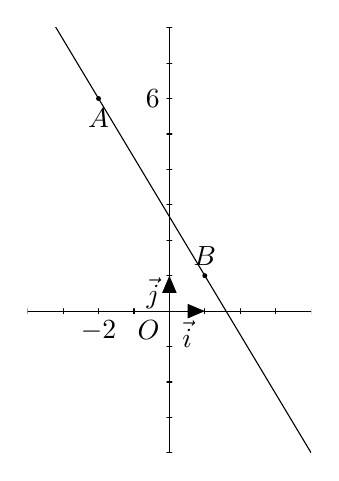
\begin{tikzpicture}[line cap=round,line join=round,>=triangle 45, scale=.45]
\clip(-4,-4) rectangle (4,8);
\draw[->,color=black] (-12.5,0) -- (9.28,0);
\foreach \x in {-12,-11,-10,-9, 8,-7, -6,-5, -4,-3, -2,-1,1, 2,3, 4,5, 6,7, 8}
\draw[shift={(\x,0)},color=black] (0pt,2pt) -- (0pt,-2pt);
\draw[->,color=black] (0,-4) -- (0,9);
\foreach \y in {-4,-3,-2,-1,1,2,3,4,5,6,7,8,9}
\draw[shift={(0,\y)},color=black] (2pt,0pt) -- (-2pt,0pt);

\draw [->] (0,0) -- (1,0);
\draw [->] (0,0) -- (0,1);
\draw (0,0) node[anchor=north east] {$O$};
\draw [domain=-17.83:9.28] plot(\x,{(8 -5*\x)/3});
% \draw [domain=-17.83:9.28] plot(\x,{(--34-10*\x)/18});

\draw (-2,0) node[below] {$-2$};


\draw (0,6) node[left] {$6$};

\draw(0.5,0) node [below]{$\vec{i}$};
\draw(0,0.5) node [left]{$\vec{j}$};

\fill (-2,6) circle (2pt);
\draw(-2,6) node [below]{$A$};

\fill  (1,1) circle (2pt);
\draw(1,1) node [above]{$B$};

\end{tikzpicture}\\
\end{center}

\underline{Résolution du système}\\

\textdbend La méthode des combinaisons linéaires est interdite. \\


$\begin{vmatrix}
10 & 6 \\ 
-5 & -3\\
\end{vmatrix}  = -30 +30 = 0 $ \\


\begin{tabular}{lp{3cm}ll}
\begin{minipage}{3cm}
$\begin{cases}
   10x +6y   \!\!\!\!\!\!\!\!&= 16\\
   -5x -3y  \!\!\!\!\!\!\!\!&=  -8\\
\end{cases}$ 
\end{minipage}  &  \multicolumn{1}{|l}{$\begin{array}{l}
                     \dfrac{1}{2}\\ -1 \\ 
                  \end{array}$ } & 
                   \begin{minipage}{3cm}
                   $\begin{cases}
                         5x +3y  \!\!\!\!\!\!\!\! &= 8\\
                         5x +3y  \!\!\!\!\!\!\!\! &= 8 \\
                   \end{cases} $ 
                \end{minipage} &  \\

\end{tabular}\\

\underline{Une seule équation} à deux inconnues\\
 Le système admet une infinité de solutions : \\

$5x +3y =8$\\
On pose $x=\lambda$ \\


\begin{minipage}{5cm}
Il vient :  \raisebox{-2ex}{$\quad \begin{cases}
               3y  \!\!\!\!\!\!\!\! &= -5\lambda  +8\\
               \; \;   y  \!\!\!\!\!\!\!\! &= -\dfrac{5\lambda +8 }{3}\\
                        \end{cases}$ }
\end{minipage}  

$S=\lbrace\lambda ,-\dfrac{5\lambda +8 }{3}\rbrace$  

\samepage

\newpage

\subsection{Systèmes se ramenant à des systèmes linéaires}

% -----------------Ex  1 Eq lin par substitution   ---------------------

\subsubsection{Exercice \no 1}

\raisebox{-2ex}{$\quad \begin{cases}
                  \dfrac{1}{x-2} + \dfrac{8}{y+5}\!\!\!\!\!\!\!\!&= 17\\
                \dfrac{7}{x-2} - \dfrac{3}{y+5} \!\!\!\!\!\!\!\! &= 1\\
                        \end{cases}$ }\\

\bigskip 

Valeurs interdites   \raisebox{-2ex}{$\quad \begin{array}{ll}
                  x\!\!\!\!\!\!\!\! &= 2\\
                  y\!\!\!\!\!\!\!\! &= -5\\
                        \end{array}$ }\\

\bigskip 


On pose :   \raisebox{-2ex}{$\quad \begin{array}{lr}
                 X \!\!\!\!\!\!\!\!&= \dfrac{1}{x-2}\\
                Y \!\!\!\!\!\!\!\!&=  \dfrac{1}{y+5}\\
                        \end{array}$ }\\
                        
\bigskip 


Le système devient  \raisebox{-2ex}{$\quad \begin{cases}
                  \;\;\; X + 8Y \!\!\!\!\!\!\!\!&= 17\\
                  7X -3Y  \!\!\!\!\!\!\!\!&= 1\\
                        \end{cases}$ }\\          
Système linéaire.             
                          
 \bigskip 
                                                           
Det = $\begin{vmatrix}
1 & 8 \\ 
7 & -3\\
\end{vmatrix}  = -3 -56 = -59 \neq 0 $ \\
  
\medskip 

\begin{tabular}{lp{3cm}ll}
\begin{minipage}{3cm}
$\begin{cases}
   \;\;\; X +8Y  \!\!\!\!\!\!\!\!&= 17\\
   7X -3Y \!\!\!\!\!\!\!\!&= 1\\
\end{cases}$ 
\end{minipage}  &  \multicolumn{1}{|l}{$\begin{array}{l}
                     3\\ 8 \\ 
                  \end{array}$ } & 
                   \begin{minipage}{3cm}
                   $\begin{cases}
                         \;\;\; X +8Y \!\!\!\!\!\!\!\!&= 17\\
                         7X -3Y  \!\!\!\!\!\!\!\!&= 1 \\
                   \end{cases} $ 
                \end{minipage} &  \multicolumn{1}{|l}{ $\begin{array}{l}
                                        -7\\~\\ 
                                  \end{array}$}\\
& & & \\
\begin{minipage}{3cm}
$\begin{cases}
   \;\;\; 3X +24Y \!\!\!\!\!\!\!\! &= 51\\
   56X -24Y \!\!\!\!\!\!\!\! &= 8\\
\end{cases}$ 
\end{minipage}  &  & 
                   \begin{minipage}{3cm}
                   $\begin{cases}
                         -7X -56Y \!\!\!\!\!\!\!\! &= -119\\
                          \quad 7X -3Y  \!\!\!\!\!\!\!\! &= 1 \\
                   \end{cases} $ 
                \end{minipage} &  \\
\cline{1-1} \cline{3-3}
\multicolumn{1}{l}{$\;\; \quad \qquad 59X=59$ } && \multicolumn{1}{r}{$\qquad \quad -59Y = -118$} & \\
$\;\;  \qquad \qquad X = 1$ && $\qquad \qquad \;\;\;\; Y = 2$ & \\
\end{tabular}\\
  
\medskip 

Il vient :\raisebox{-10ex}{
\begin{tabular}{rp{2cm}r}
$ \dfrac{1}{x-2}=1$ & & $ \dfrac{1}{y+5}= 2$  \\
&& \\
$x-2=1$ && $2(y+5)=1$ \\
$x=3$ && $2y+10 = 1$ \\
\underline{Convient} && $2y=-9$ \\
         && $y=-\dfrac{9}{2}$\\
         && \underline{Convient}\\
\end{tabular}}\\

  
\medskip 

$S=\left\lbrace(3 ,-\dfrac{9 }{2})\right\rbrace$  

\newpage

% -----------------Ex 2 Eq lin par substitution   ---------------------

\subsubsection{Exercice \no 2}
\raisebox{-2ex}{$\quad \begin{cases}
                    4 (x-3)^{2}  -3(y+2)^{2}\!\!\!\!\!\!\!\! &= -83\\
                    6 (x-3)^{2} +11(y+2)^{2}\!\!\!\!\!\!\!\! &= 635\\
                        \end{cases}$ }\\

\bigskip 

On pose :   \raisebox{-2ex}{$\quad \begin{array}{lr}
                 X \!\!\!\!\!\!\!\!&= (x-3)^{2}\\
                Y \!\!\!\!\!\!\!\!&=  (y+2)^{2}\\
                        \end{array}$ }\\
                        

\bigskip 

Le système devient  \raisebox{-2ex}{$\quad \begin{cases}
                  \;\;\; 4X  -3Y \!\!\!\!\!\!\!\!&= -83\\
                  6X +11Y \!\!\!\!\!\!\!\!&= 635\\
                        \end{cases}$ }\\            

\bigskip 
                                               
Det = $\begin{vmatrix}
4 & -3 \\ 
6 & 11\\
\end{vmatrix}  = 44 + 18 = 62 \neq 0 $ \\
  

\bigskip 

\begin{tabular}{lp{3cm}ll}
\begin{minipage}{3cm}
$\begin{cases}
   \;\;\;4X -3Y \!\!\!\!\!\!\!\!&= -83\\
   6X +11Y \!\!\!\!\!\!\!\!&= 635\\
\end{cases}$ 
\end{minipage}  &  \multicolumn{1}{|l}{$\begin{array}{l}
                     11\\ 3 \\ 
                  \end{array}$ } & 
                   \begin{minipage}{3cm}
                   $\begin{cases}
                         \;\;\; 4X  -3Y \!\!\!\!\!\!\!\!&= -83\\
                         6X +11Y \!\!\!\!\!\!\!\!&= 635 \\
                   \end{cases} $ 
                \end{minipage} &  \multicolumn{1}{|l}{ $\begin{array}{l}
                                        -3\\2\\ 
                                  \end{array}$}\\
& & & \\
\begin{minipage}{3cm}
$\begin{cases}
   44X   -33Y \!\!\!\!\!\!\!\! &= -913\\
   18X   +33Y \!\!\!\!\!\!\!\!&= 1905\\
\end{cases}$ 
\end{minipage}  &  & 
                   \begin{minipage}{3cm}
                   $\begin{cases}
                         -12X + 9Y  \!\!\!\!\!\!\!\!&= 249\\
                          12X +22Y  \!\!\!\!\!\!\!\!&= 1270 \\
                   \end{cases} $ 
                \end{minipage} &  \\
\cline{1-1} \cline{3-3}
\multicolumn{1}{l}{$\;\; \quad \qquad 62X=992$ } && \multicolumn{1}{r}{$31Y = 1519$} & \\
$\qquad \qquad \; \; X = 16$ && $\qquad \qquad \quad  Y = 49$ & \\
\end{tabular}\\

\bigskip 

Il vient : \raisebox{-8ex}{
\begin{tabular}{rp{2cm}r}
$ (x-3)^{2}=16$ & \multicolumn{1}{c}{et} & $ (y+2)^{2} = 49$  \\
&& \\
$(x-3)^{2} -16 = 0$ && $(y+2)^{2}-49 = 0$ \\
$(x-3+4)(x-3-4) = 0 $ && $(y+2+7)(y+2-7) = 0$ \\
$(x+1)(x-7) = 0 $ && $(y+9)(y-5) = 0$ \\
$x+1 = 0 \textrm{ ou } x-7 = 0 $ && $y +9 = 0 \textrm{ ou } y -5 = 0$ \\
$x = -1 \textrm{ ou } x = 7 $ && $y = -9 \textrm{ ou } y = 5 $ \\
\end{tabular}}\\


\bigskip 

$S=\left\lbrace(-1 ,-9), (-1, 5), (7, -9), (7, 5)\right\rbrace$  

Le système admet 4 couples de solutions.

\newpage



\subsection{Algorithmique}
\subsubsection{Colinéarité de deux vecteurs}

Soit $(O, \vec{i}, \vec{j})$ un repère.
\smallskip
Soit $ A(x_A, y_A) \quad B(x_B, y_B) \quad C(x_C, y_C) \quad D(x_D, y_D) $
 
\begin{tabular}{l|l}
\multicolumn{2}{c}{~} \\
\parbox{9cm}{\vspace{.5cm}
\ding{43} \underline{Saisir}
    \raisebox{-5.5ex}{\hspace*{.5cm}\parbox{0.5\columnwidth}{%                        
                  $x_{A}, y_{A},$\\
                  $x_{B}, y_{B},$  \\
                  $x_{C}, y_{C},$  \\
                  $x_{D}, y_{D} $  \\
                  }}}   & 
                           \begin{minipage}{0.8\columnwidth}
        %                   \underline{Prog} 
                            
        %                   \raisebox{-10ex}{   
                           \fcolorbox{ecranTI}{ecranTI}{\parbox{3cm}
                           { \small
                                \texttt{PROGRAM:COLINE}\\
                                \texttt{:Input "XA : ",X}\\
                                \texttt{:Input "YA : ",Y}\\
                                \texttt{:Input "XB : ",Z}\\
                                \texttt{:Input "YB : ",T}\\
                                \texttt{:Input "XC : ",S}\\
                                \texttt{:Input "YC : ",U}\\
                                \texttt{:Input "XD : ",V}\\
                                \texttt{:Input "YD : ",W}\\
                           }}
        %                   }
        \smallskip
                         \end{minipage} \\
& \\
& \\
\parbox{8cm}{\medskip
\ding{43} \underline{Traitement} $\overrightarrow{AB}\left(\begin{array}{l} x_B-x_A\\
y_B-y_A\\
\end{array} \right)  \quad \left(\begin{array}{l} 
                              x_D-x_C\\
                              y_D-y_C\\
                        \end{array} \right)$\\
                        
    \begin{minipage}{\columnwidth}%    
              \begin{tabular}{rl}
                 $x_{B}-x_{A}$ & donne la valeur $a$\\%
                 $y_{B}-y_{A}$ & donne la valeur $b$\\%
                 $x_{D}-x_{C}$ & donne la valeur $c$\\%
                 $y_{D}-y_{C}$ & donne la valeur $d$\\%

              \end{tabular}  
          \end{minipage} \\
            }    & 
\begin{minipage}{0.8\columnwidth}
    %\vspace*{-2cm}      
\fcolorbox{ecranTI}{ecranTI}{\parbox{3cm}
{ \small
\texttt{:Z-X$\rightarrow$A}\\
\texttt{:T-Y$\rightarrow$B}\\
\texttt{:V-S$\rightarrow$C}\\
\texttt{:W-U$\rightarrow$D}\\
}}
\smallskip
  \end{minipage} \\
 & \\
\parbox{6cm}{
    \begin{minipage}{\columnwidth}%    
 $(x_B-x_A)(y_D-y_c)-(y_B-y_A)(x_D-x_C)$ prend la valeur $e$\\
\medskip 
$\begin{vmatrix}
   x_B - x_A & x_D - x_C \\
   y_B - y_A & y_D - y_C\\
\end{vmatrix}  = e $             
    \end{minipage} \\
            }    & 
\begin{minipage}{0.8\columnwidth}
    %\vspace*{-2cm}      
\fcolorbox{ecranTI}{ecranTI}{\parbox{3cm}
{ \small
\texttt{:A*D-B*C$\rightarrow$E}\\
}}
\smallskip
  \end{minipage} \\ 
& \\
& \\  
\parbox{8cm}{\medskip
\ding{43} \underline{Sorties} $\quad e=0 \Longleftrightarrow \overrightarrow{AB}$ et $\overrightarrow{CD}$ sont colinéaires\\

    \begin{minipage}{\columnwidth}%           
        Si $e = 0 $ \\
        \hspace *{.5cm} Afficher "OUI"\\
        Sinon\\
         \hspace *{.5cm} Afficher "NON"\\
        fin de Si       
     \end{minipage} \\
            }    & 
\begin{minipage}{0.8\columnwidth}    
\fcolorbox{ecranTI}{ecranTI}{\parbox{3cm}
{ \small
\texttt{:IF E=0}\\
\texttt{:Disp "OUI"}\\
\texttt{:ELSE}\\
\texttt{:Disp "NON"}\\
\texttt{:End}
}}
  \end{minipage} \\
\end{tabular} \\

\newpage

\subsection{Exemples de problèmes}

\bigskip 

\begin{enumerate}
\reversemarginpar 

% -----------------Ex  1 Eq lin Nombreux exemples  ---------------------

\item \marginpar[\underline{Ex \no 1}]~ \underline{ Énoncé }:\\

Chez un confiseur, Sylvette achète des chocolats noirs et des chocolats blancs au détail.\\

Chaque chocolat noir est vendu 0,45\euro et pèse 35g.\\
Chaque chocolat blanc est vendu 0,30\euro et pèse 20g. \\

Sylvette paie 13,80\euro pour 980g de chocolat. \\

Déterminer le nombre de chocolats de chaque sorte achetés par Sylvette.\\


\bigskip 

\marginpar[{\it Choix des inconnues}]
~\parbox{9cm}{Soit $x$ le \underline{nombre} de chocolats noirs.\\
Soit $y$ le \underline{nombre} de chocolats blancs.}

\bigskip 

\item \underline{Mise en équation du problème :  }\\

$\begin{cases}
0,45x + 0,30y \!\!\!\!\!\!\!\! &= 13,80\\
\qquad 35x + 20y     \!\!\!\!\!\!\!\! &= 980\\
\end{cases}$ \\

\bigskip 

\item \underline{Résolution du système : }\\

\begin{tabular}{lp{3cm}ll}
\begin{minipage}{4cm}
$\begin{cases}
  0,45x + 0,30y \!\!\!\!\!\!\!\! &= 13,80\\
  \qquad  35x + 20y \!\!\!\!\!\!\!\! &= 980\\
\end{cases}$ 
\end{minipage}  &  \multicolumn{1}{|l}{$\begin{array}{l}
                     200\\ -3 \\ 
                  \end{array}$ } & 
                   \begin{minipage}{4cm}
                   $\begin{cases}
                        0,45x + 0,30y \!\!\!\!\!\!\!\! &= 13,80\\
                        \qquad  35x + 20y\!\!\!\!\!\!\!\! &= 980\\
                   \end{cases} $ 
                \end{minipage} &  \multicolumn{1}{|l}{ $\begin{array}{l}
                                        -35\\0,45\\ 
                                  \end{array}$}\\
& & & \\
\begin{minipage}{3cm}
$\begin{cases}
   \quad 30x   +60y \!\!\!\!\!\!\!\!&= 2760\\
   -105x -60y \!\!\!\!\!\!\!\! &= -2940\\
\end{cases}$ 
\end{minipage}  &  & 
                   \begin{minipage}{3cm}
                   $\begin{cases}
                        -15,75x -10,5y \!\!\!\!\!\!\!\!&= -483\\
                         \qquad  15,75x  +3Y   \!\!\!\!\!\!\!\!&= 441\\
                   \end{cases} $ 
                \end{minipage} &  \\
\cline{1-1} \cline{3-3}
\multicolumn{1}{l}{$\qquad \qquad \;  -15x = -180$ } && \multicolumn{1}{l}{$\qquad \qquad \quad \;\;\;  -1,5y = -42$} & \\
$\qquad \qquad \qquad \; x = 12$ && $\qquad \qquad \qquad \quad \;\;\;\; y = 28$ & \\
\end{tabular}\\


\begin{tabular}{lp{3cm}ll}
\begin{minipage}{4cm}
$\begin{cases}
 3x + 2y  \!\!\!\!\!\!\!\!&= 92\\
   7x + 4y \!\!\!\!\!\!\!\!&= 196\\
\end{cases}$ 
\end{minipage}  &  \multicolumn{1}{|l}{$\begin{array}{l}
                     -2\\ ~ \\ 
                  \end{array}$ } & 
                   \begin{minipage}{4cm}
                   $\begin{cases}
                        3x + 2y  \!\!\!\!\!\!\!\!&= 92\\
                          7x + 4y \!\!\!\!\!\!\!\!&= 196\\
                   \end{cases} $ 
                \end{minipage} &  \multicolumn{1}{|l}{ $\begin{array}{r}
                                        7\\-3\\ 
                                  \end{array}$}\\
& & & \\

\multicolumn{1}{l}{$x = 12$  } && \multicolumn{1}{l}{$2y = 56$ } & \\
&& $y = 28$ & \\
\end{tabular}\\

\item \underline{Réponse :} Sylvette a acheté 12 chocolats noirs et 28 chocolats blancs.
  
 
\end{enumerate}

\newpage 

\begin{enumerate}
\reversemarginpar 
% -----------------Ex  2 Eq lin Nombreux exemples  ---------------------
\item \marginpar[\underline{Ex \no 2}]~ \underline{ Énoncé }:\\

\begin{itemize}
\item [*] Si l'on augmente de $2m$ la longueur $L$ d'un rectangle et de $3m$ sa largeur $l$, alors l'aire du rectangle augmente de $36m^{2}$.
\item [*] Si l'on diminue $L$ de $5m$ et $l$ de $4m$, alors l'aire diminue de $135m^{2}$. 
\end{itemize}

Quelles sont les dimensions initiales du rectangle ? 

\bigskip 

\marginpar[{\it Choix des inconnues}]
~\parbox{9cm}{Soit $L$ la longueur initiale du rectangle et $l$ la largeur initiale du rectangle ; unité : le mètre.}

\bigskip 

\item \underline{Mise en équarion du problème :  }\\

$\begin{cases}
(L+2)(l+3) \!\!\!\!\!\!\!\!&= L{\times}l + 96 \\
(L-5)(l-4) \!\!\!\!\!\!\!\!&= L{\times}l -135 \\
\end{cases}$ \\


\item \underline{Résolution du système : }\\


\begin{tabular}{lp{3cm}ll}
\multicolumn{4}{l}{
$\begin{cases}
(L+2)(l+3)\!\!\!\!\!\!\!\! &= L{\times}l + 96 \\
(L-5)(l-4) \!\!\!\!\!\!\!\!&= L{\times}l -135 \\
\end{cases}$} \\
& & & \\
\multicolumn{4}{l}{
$\begin{cases}
\;\; Ll +3L +2l +6  \!\!\!\!\!\!\!\!&= Ll + 96 \\
Ll -4L -5l +20 \!\!\!\!\!\!\!\!&= Ll -135 \\
\end{cases}$ } \\
& & & \\
\begin{minipage}{4cm}
$\begin{cases}
\;\; \; 3L +2l  \!\!\!\!\!\!\!\!&= \quad 90 \\
-4L -5l \!\!\!\!\!\!\!\!&= -155 \\
\end{cases}$ \\

\end{minipage}  &  \multicolumn{1}{|l}{$\begin{array}{l}
                     5\\ 2 \\ 
                  \end{array}$ } & 
                   \begin{minipage}{4cm}       
                         $\begin{cases}
                             \;\; \; 3L +2l  \!\!\!\!\!\!\!\!&= \quad 90 \\
                            -4L -5l \!\!\!\!\!\!\!\!&= -155 \\
                          \end{cases}$ 
                \end{minipage} &  \multicolumn{1}{|l}{ $\begin{array}{l}
                                        4\\3\\ 
                                  \end{array}$}\\
& & & \\
\begin{minipage}{3cm}
$\begin{cases}
15L + 10l \!\!\!\!\!\!\!\! &= 450\\
-8L -10l \!\!\!\!\!\!\!\! &= -310 \\
\end{cases}$ 
\end{minipage}  &  & 
                   \begin{minipage}{3cm}
                   $\begin{cases}
                        \quad 12L + 8l \!\!\!\!\!\!\!\! &= 360 \\
                       -12L -15l \!\!\!\!\!\!\!\!  &= -465\\
                   \end{cases} $ 
                \end{minipage} &  \\
\cline{1-1} \cline{3-3}
\multicolumn{1}{l}{$\qquad \qquad 7L = 140 $ } && \multicolumn{1}{l}{$\qquad \qquad -7L = -105$} & \\
$\qquad \qquad \; \; \;  L = 20 $ && $\qquad \qquad \quad \; \;  l = 15$ & \\
\end{tabular}\\


\bigskip 

\item \underline{Réponse au problème } :\\

      La longueur initiale était de $20m$ et la largeur initiale de $15m$ 

  
  
\end{enumerate}

  \newpage
  

\begin{enumerate}
\reversemarginpar 
% -----------------Ex  3 Eq lin Nombreux exemples  ---------------------

\vspace*{-1cm}
\item \marginpar[\underline{Ex \no 3}]~ \underline{ Énoncé }:\\

Soit $(0,\vec{i}, \vec{j})$ un repère orthonormal.

Soient $A(6,3) \quad B(-2,-7) \quad C (16,-1)$ 

Soit $\Omega$ le centre du cercle circonscrit au triangle $ABC$.

Déterminer les coordonnées du point $\Omega$.\\



\begin{tabbing}
On a \hspace*{1cm}\= $\Omega{A} = \Omega{B} = \Omega{C}$ \\ 
     \> $ \Longleftrightarrow  \begin{cases}
                        \Omega{A}\!\!\!\!\!\!\!\! &= \Omega{B} \\
                        \Omega{A} \!\!\!\!\!\!\!\!&= \Omega{C} \\
                   \end{cases} $ \\
     \> $ \Longleftrightarrow \begin{cases}
                        \Omega{A}^{2} \!\!\!\!\!\!\!\! &= \Omega{B}^{2} \\
                        \Omega{A}^{2} \!\!\!\!\!\!\!\! &= \Omega{C}^{2} \\
                   \end{cases} $ \\
\end{tabbing}

\marginpar[{\it Choix des inconnues}]
~\parbox{9cm}{Soit $x$ l'abscisse de $\Omega$ \\
              Soit $y$ l'ordonnée de $\Omega$}\\

\item \underline{Mise en équation du problème :  }\\


$\overrightarrow{\Omega{A}}\left( \begin{array}{l}
                     6-x\\ 9-y\\ 
                  \end{array} \right) \quad  
         \overrightarrow{\Omega{B}} \left( \begin{array}{l}
                     -2-x\\ -7-y\\ 
               \end{array} \right)  \quad   
             \overrightarrow{\Omega{C}}\left( \begin{array}{l}
                     16-x\\ -1-y\\ 
                  \end{array} \right) $ \\
 
$\begin{array}{r@{\;}l}
   \Omega{A}^{2} &= (6 - x)^{2} + (9 - y)^{2} \\
   \Omega{B}^{2} &= (-2 - x)^{2} + (-7 - y)^{2} \\
   \Omega{C}^{2} &= (16 - x)^{2} + (-1- y)^{2} \\   
\end{array}$ \\

$\begin{cases}
 (6 - x)^{2} + (9 - y)^{2} \!\!\!\!\!\!\!\! &= (-2 - x)^{2} + (-7 - y)^{2} \\
 (6 - x)^{2} + (9 - y)^{2} \!\!\!\!\!\!\!\! &= (16 - x)^{2} + (1- y)^{2} \\
\end{cases} $\\               
 
\item \underline{Résolution du système : }

\begin{tabular}{lp{3cm}ll}
\multicolumn{4}{l}{
$\begin{cases}
36 -12x\ \cancel {+x^2} +81 -18y \ \cancel {+y^2}  
 \!\!\!\!\!\!\!\! &= 4 + 4x\ \cancel {+x^2} +49 +14y \ \cancel {+y^2} \\
36 -12x\ \cancel {+x^2} +81 -18y \ \cancel {+y^2} 
 \!\!\!\!\!\!\!\! &= 256 -32x\ \cancel {+x^2} +1 +2y \ \cancel {+y^2}  \\
\end{cases}$} \\
& & & \\
\multicolumn{4}{l}{
$\begin{cases}
-12x -18y +117  \!\!\!\!\!\!\!\! &= 4x +14y +53 \\
-12x -18y +117 \!\!\!\!\!\!\!\!  &= -32x +2y +257 \\
\end{cases}$} \\
& & & \\
\multicolumn{4}{l}{
$\begin{cases}
-16x -32y \!\!\!\!\!\!\!\! &= -64\\
\quad 20x -20y  \!\!\!\!\!\!\!\! &= 140 \\
\end{cases}$ } \\
& & & \\
\begin{minipage}{4cm}
$\begin{cases}
x +2y   \!\!\!\!\!\!\!\! &= 4 \\
\;\; x -y    \!\!\!\!\!\!\!\! &= 7 \\
\end{cases}$ \\
\end{minipage}  &  \multicolumn{1}{|l}{$\begin{array}{l}
                     ~\\ 2 \\ 
                  \end{array}$ } & 
                   \begin{minipage}{4cm}       
                         $\begin{cases}
                             x +2y   \!\!\!\!\!\!\!\!&= 4 \\
                             \;\; x -y   \!\!\!\!\!\!\!\!  &= 7 \\
                          \end{cases}$ 
                \end{minipage} &  \multicolumn{1}{|l}{ $\begin{array}{l}
                                        ~\\-1\\ 
                                  \end{array}$}\\
& & & \\
\begin{minipage}{3cm}
$\begin{cases}
\; \; x +2y \!\!\!\!\!\!\!\!  &=  4 \\
 2x -2y  \!\!\!\!\!\!\!\!  &= 14 \\
\end{cases}$ 
\end{minipage}  &  & 
                   \begin{minipage}{3cm}
                   $\begin{cases}
                         \; \; x +2y  \!\!\!\!\!\!\!\!  &=  4 \\
                       -x +y   \!\!\!\!\!\!\!  &= -7 \\
                   \end{cases} $ 
                \end{minipage} &  \\
\cline{1-1} \cline{3-3}
\multicolumn{1}{l}{$\qquad \quad 2x=18$ } && \multicolumn{1}{l}{$\qquad \; \; \;\;   3y = -3$} & \\
$\qquad \quad \; \; \; x = 6$ && $ \qquad \quad \;  y = -1$& \\
\end{tabular}

\item \underline{Réponse au problème } :\\

$\Omega (6, -1) $ 
  
\end{enumerate}

  \newpage  
  
\begin{enumerate}
\reversemarginpar 
% -----------------Ex  4 Eq lin Nombreux exemples  ---------------------
\item \marginpar[\underline{Ex \no 4}]~ \underline{ Énoncé }:\\

Deux motocyclistes (Sylvain et Sylvette) quittent simultanément une ville $A$ et se dirigent vers une ville $B$\\

Sylvain arrive en $B$ à 12h. Il a roulé à 80km/h.\\
Sylvette arrive en $B$ à 13h. Elle a roulé à 60km.h$^{-1}$.\\

Déterminer la distance entre $A$ et $B$ et l'heure de départ des deux motocyclistes.

\marginpar[{\it Choix des inconnues}]
~\parbox{9cm}{Soit $d$ la distance entre $A$ et $B$. Unité : km \\
              Soit $h$ l'heure de départ des deux motocyclistes}\\

\item \underline{Mise en équation du problème :  }\\

$v = \dfrac{d}{t}$ en km$\times$ heure$^{-1} \quad d=vt \quad t=\dfrac{d}{v}$ \\



\item \underline{Résolution du système : }

\begin{tabular}{lp{3cm}ll}
\multicolumn{4}{l}{
$\begin{cases}
d  \!\!\!\!\!\!\!\! &= 80 \times (12-h) \\
d  \!\!\!\!\!\!\!\! &= 60 \times (13-h) \\
\end{cases}$} \\
& & & \\
\multicolumn{4}{l}{
$\begin{cases}
-960 \!\!\!\!\!\!\!\!  &= -d -80h  \\
-780 \!\!\!\!\!\!\!\!  &= -d -60h \\
\end{cases}$} \\
& & & \\
\begin{minipage}{4cm}
$\begin{cases}
d +80h \!\!\!\!\!\!\!\! &= 360 \\
d +60h \!\!\!\!\!\!\!\! &= 780\\
\end{cases}$ \\
\end{minipage}  &  \multicolumn{1}{|l}{$\begin{array}{l}
                     3\\ -4 \\ 
                  \end{array}$ } & 
                   \begin{minipage}{4cm}       
                         $\begin{cases}
                             d +80h \!\!\!\!\!\!\!\! &= 360 \\
                             d +60h \!\!\!\!\!\!\!\! &= 780\\
                          \end{cases}$ 
                \end{minipage} &  \multicolumn{1}{|l}{ $\begin{array}{l}
                                        ~\\-1\\ 
                                  \end{array}$}\\
& & & \\
\begin{minipage}{3cm}
$\begin{cases}
 \;\;\; 3d +240h \!\!\!\!\!\!\!\!    &=  2880 \\
-4d -240h \!\!\!\!\!\!\!\!   &= -3120 \\
\end{cases}$ 
\end{minipage}  &  & 
                   \begin{minipage}{3cm}
                   $\begin{cases}
                        \;\;\; d +80h  \!\!\!\!\!\!\!\!   &=   360\\
                       -d -60h  \!\!\!\!\!\!\!\!   &=  -780\\
                   \end{cases} $ 
                \end{minipage} &  \\                
\cline{1-1} \cline{3-3}
\multicolumn{1}{l}{$\qquad \qquad \; \; \;  -d=-240$  } && \multicolumn{1}{l}{$\qquad \quad 20h = 180$} & \\
$\qquad \qquad \quad \; \;   d = 240$ && $ \qquad \qquad h = 9h$& \\
\end{tabular}

\item \underline{Réponse au problème } :\\

La distance parcourue est de 240 km et l'heure de départ est 9h.
  
\end{enumerate}



  \newpage  

\begin{enumerate}
\reversemarginpar 

\item \marginpar[\underline{Ex \no 5}]~ \underline{ Énoncé }:\\
% -----------------Ex  5 Eq lin Nombreux exemples  ---------------------
Sylvain et Sylvette vont en voiture de $A$ à  $B$. Le trajet comporte une partie de route et une partie d'autoroute.

\hspace*{2cm}\begin{tabular}{l|c|c}
 & Route & Autoroute \\
 \hline
\parbox{3cm}{\smallskip Vitesse\\ (en km.h$^{-1}$)\smallskip } & 90 & 130 \\
 \hline
\parbox{3cm}{\smallskip Consommation\\ d'essence\\ (litres/100km)\smallskip } & 6,5 & 9 \\
  
\end{tabular}\\

Sylvain et Sylvette ont mis 1h50 et ont consommé 13,5l d'essence.\\
Déterminez la longueur totale du trajet.\\


\marginpar[{\it Choix des inconnues}]
~\parbox{9cm}{Soit $x$ la longueur de partie route du trajet.\\
              Soit $y$ la longueur de partie autoroute du trajet.\\
              \underline{Unité} : le kilomètre.}\\

\item \underline{Mise en équation du problème :  }\\

\begin{minipage}{2.8cm}
\flushright Temps : 

\bigskip

\medskip 

Consommation :
\end{minipage}               
$\begin{cases}
\qquad \dfrac{x}{30} +\dfrac{y}{130} \!\!\!\!\!\!\!\!  &= \dfrac{11}{6}  \\
 & \\
\dfrac{6,5}{100} x +\dfrac{9}{100} y \!\!\!\!\!\!\!\! &= 13,5  \\
\end{cases}$\\

\item \underline{Résolution du système : }\\

\begin{tabular}{lp{3cm}ll}
\multicolumn{4}{l}{
$\begin{cases}
\quad \quad \dfrac{x}{90} +\dfrac{y}{130} \!\!\!\!\!\!\!\! &= \dfrac{11}{6}  \\
& \\
\dfrac{6,5}{100} x +\dfrac{9}{100} y\!\!\!\!\!\!\!\!  &= 13,5  \\
\end{cases}$} \\
& & & \\
\multicolumn{4}{l}{
$\begin{cases}
\dfrac{13x}{117} +\dfrac{9y}{117}\!\!\!\!\!\!\!\!  &= \dfrac{11}{6}  \\
         \; \; \; 6,5x    +9y \!\!\!\!\!\!\!\! &= 1950  \\
\end{cases}$} \\
& & & \\
\multicolumn{4}{l}{
$\begin{cases}
78x + 54y\!\!\!\!\!\!\!\! &= 12870  \\
6,5x    +9y \!\!\!\!\!\!\!\! &= 1950  \\
\end{cases}$} \\
& & & \\
\begin{minipage}{4cm}
$\begin{cases}
39x + 27y \!\!\!\!\!\!\!\! &= 6435  \\
6,5x    +9y \!\!\!\!\!\!\!\! &= 1950  \\
\end{cases}$ \\
\end{minipage}  &  \multicolumn{1}{|l}{$\begin{array}{l}
                     ~\\ -3 \\ 
                  \end{array}$ } & 
                   \begin{minipage}{4cm}       
                         $\begin{cases}
                            39x + 27y \!\!\!\!\!\!\!\! &= 6435  \\
                           6,5x    +9y \!\!\!\!\!\!\!\! &= 1950  \\
                          \end{cases}$ 
                \end{minipage} &  \multicolumn{1}{|l}{ $\begin{array}{l}
                                        ~\\-6\\ 
                                  \end{array}$}\\
& & & \\               
\cline{1-1} \cline{3-3}
\multicolumn{1}{l}{$\qquad \; \;  19,5x = 585$} && \multicolumn{1}{l}{$\qquad  \; \; -27y =-5265$}&\\
$\qquad \qquad \; \; \; x = 30$ && $\qquad \qquad \; \; \; y = 195$& \\
\end{tabular}

\item \underline{Réponse au problème } :\\

Sylvain et Sylvette ont parcouru : $30 + 195 = 225$Km au total.
  
\end{enumerate}

\newpage
% -----------------Ex 6 Eq lin Nombreux exemples  ---------------------

\begin{enumerate}
\reversemarginpar 

\item \marginpar[\underline{Ex \no 6}]~ \underline{ Énoncé }:\\

Deux villes $A$ et $B$ sont distantes de 130km.

Sylvain part à 8h de $A$ et se dirige vers $B$.\\
Sylvette\ding{172} part à 9h de $B$ et se dirige vers $A$.\\
Sylvette\ding{173} part à 9h30 de $B$ et se dirige vers $A$.\\
Les deux Sylvettes  à la même vitesse.\\
Sylvain rencontre Sylvette\ding{172} après avoir parcouru 88km\\ 
Sylvain rencontre Sylvette\ding{173} après avoir parcouru 106km\\ 
Déterminer la vitesse de Sylvain et la vitesse des Sylvettes.

\item  \underline{Choix des inconnues} \\

$\left. \begin{array}{l}
      \text{Soit } V_1 \text { la vitesse de Sylvain.}\\
      \text {Soit } V_2 \text { la vitesse des Sylvettes.}
\end{array}         
 \right\rbrace V_1 \text{ et } V_2 \text { en km/h}. $        

\medskip             

\item \underline{Mise en équation du problème :  }\\
\begin{itemize}
\item [\ding{87}] \raisebox{-1.6ex}{\parbox{5cm}{Temps mis par Sylvain \\
jusqu'à la première rencontre} :$\qquad \dfrac{88}{V_1}$} \\

~\raisebox {-1.6ex}{\parbox{5cm}{Temps mis par Sylvette\ding{172}\\ 
jusqu'à la première rencontre}  :$\qquad \dfrac{42}{V_2}$ }
\marginpar[{\flushright \it Et alors}] ~\\

\item [\ding{87}] \raisebox {-1.6ex}{\parbox{5cm}{Temps mis par Sylvain \\
jusqu'à la deuxième rencontre} :$\qquad \dfrac{106}{V_1}$} \\

~\raisebox {-1.6ex}{\parbox{5cm}{Temps mis par Sylvette\ding{173}\\
jusqu'à la deuxième rencontre} :$\qquad \dfrac{24}{V_2}$ }
\marginpar[{\flushright  \it Et alors}] ~
\end{itemize}

\medskip             

On a : $\left\{ \begin{array}{l@{\;}ll}
8+\dfrac{88}{V_{1}} & =9+\dfrac{42}{V_{2}} & \longleftarrow\textrm{Heure de la première rencontre}\\
& & \\
8+\dfrac{106}{V_{1}} & =9,5+\dfrac{24}{V_{2}} & \longleftarrow\textrm{Heure de la deuxième rencontre}\\
\end{array}\right.$\\

\bigskip 

\centerline {\includegraphics[width=.6\textwidth]{Sylvain+Sylvette_Course.jpg}} 
\newpage           

\item \underline{Résolution du système : }\\

\begin{tabular}{lp{3.5cm}ll}
\multicolumn{4}{l}{
$\begin{cases}
\qquad\dfrac{88}{V_1} -\dfrac{42}{V_2} \!\!\!\!\!\!\!\! &= 1 \\
& \\
\dfrac{106}{V_1} x -\dfrac{24}{V_2} y \!\!\!\!\!\!\!\!&= 1,5  \\
\end{cases}$} \\
& & & \\
\multicolumn{4}{l}{
Le système est linéaire si l'on pose :
       $X=\dfrac{1}{V_1} \text{ et }  Y=\dfrac{1}{V_2}$}\\
& & & \\
\begin{minipage}{4cm}
$\begin{cases}
 \; \; \; 88X - 42Y \!\!\!\!\!\!\!\!&= 1 \\
106X - 24Y\!\!\!\!\!\!\!\! &= 1,5  \\
\end{cases}$ \\
\end{minipage}  &  \multicolumn{1}{|l}{$\begin{array}{l}
                     24\\ -42 \\ 
                  \end{array}$ } & 
                   \begin{minipage}{4cm}       
                         $\begin{cases}
                             \; \; \; 88X - 42Y \!\!\!\!\!\!\!\!&= 1 \\
                            106X - 24Y \!\!\!\!\!\!\!\!&= 1,5  \\
                          \end{cases}$ 
                \end{minipage} &  \multicolumn{1}{|l}{ $\begin{array}{l}
                                        106\\-88\\ 
                                  \end{array}$}\\
& & & \\   
\begin{minipage}{4cm}
$\begin{cases}
 \quad 2112X - 1008Y \!\!\!\!\!\!\!\!&= 24 \\
-4452X - 1008Y \!\!\!\!\!\!\!\!&= -63  \\
\end{cases}$ \\
\end{minipage}  &  & 
                   \begin{minipage}{4cm}       
                         $\begin{cases}
                             \quad 9328X - 4452Y \!\!\!\!\!\!\!\!&= 106 \\
                            -9328X + 2112Y \!\!\!\!\!\!\!\!&= -132  \\
                          \end{cases}$ 
                \end{minipage} &  \\
& & & \\                           
\cline{1-1} \cline{3-3}
\multicolumn{1}{l}{$\qquad \qquad \; \; \; -2340X = -39$} &&
               \multicolumn{1}{l}{$\qquad \qquad \; \; \; -2340Y =-26$}&\\
$\qquad \qquad \qquad \quad \;\; \; X = \dfrac{1}{60}$ && $\qquad \qquad \qquad \quad \;  \; \; Y = \dfrac{1}{90}$& \\
\end{tabular}\\

Il vient : $\dfrac{1}{V_1} = \dfrac{1}{60} $ 
       et  $\dfrac{1}{V_2} = \dfrac{1}{90} $\\


\item \underline{Réponse au problème } :\\

Sylvain roule à 60km/h et les 2 Sylvettes à 90km/h.
  
\end{enumerate}   \newpage $\;$ \newpage

\section{Trigonométrie}
\subsection{Cercle trigonométrique}
On appelle cercle trigonométrique tout cercle de rayon $R=1$ sur lequel on a choisi une origine $I$ et un sens de parcours appelé « sens trigonométrique ». 

%------------- Cerlcle trigonométrique ------------------

\hspace*{2cm}
\begin{tikzpicture}[line cap=round,line join=round,>=triangle 45,x=1.0cm,y=1.0cm,scale=.8]
\clip(-3,-3) rectangle (3,3);
\draw [color=gray] (0,0) circle (2cm);
\draw (0,0)-- (2,0);
\draw [shift={(0,0)}] plot[domain=0.17:1.12,variable=\t]({1*2.35*cos(\t r)+0*2.35*sin(\t r)},{0*2.35*cos(\t r)+1*2.35*sin(\t r)});
\draw [->] (1.05,2.1) -- (1.03,2.11);
\fill (0,0) circle (1.5pt);
\draw (0,0) node [below]{$O$};
\fill (2,0) circle (1.5pt);
\draw(2,0) node [right] {$I$};
% \draw (-1/2, sqrt(3)/2) node [left] {$I'$};
\end{tikzpicture}\raisebox{10ex}{$R=OI=1$}
 
\subsection{Image d'un nombre réel sur le cercle trigonométrique}

Soit $\mathcal{C}$ un cercle trigonométrique.

$\mathcal{P} = 2{\pi}R = 2\pi \text{ puisque } R=1$ \\ 

\begin{itemize}
\item [\ding{87}] À tout nombre réel $x$ correspond un point et un seul de $\mathcal{C}$ appelé « image de $x$ sur $\mathcal{C}$ 
noté $M(x)$.\\

$M(\pi) = I'$ 
\item [\ding{87}] Tout point $M$ de  $\mathcal{C}$ est l'image d'une infinité de nombres réels.

\begin{minipage}{9cm}
\begin{tabbing}
Si \= $M$ est $\qquad\quad$ \= l'image de $x$ sur  $\mathcal{C}$\\
   \>  $M$ est aussi \> l'image de $x+2\pi$ \\
   \>  $M$ est aussi \> l'image de $x+4\pi$ \\  
   \>  $M$ est aussi \> l'image de $x+6\pi$\ldots  \\   
   \>  $M$ est aussi \> l'image de $x+2k\pi \quad k\in \mathbb{Z}$ \\    
\end{tabbing}
\hspace*{5cm}
\end{minipage}
%
%------- Enroulement des réels sur le cercle trigo --------
% Pour tracer les courbes de Bésier : 
% ajouter, 
% 1 - dans les préférences de TexMaker, 
%     dans  la ligne  pdflatex 
%     "--shell-escape  -enable-write18 " avant "%.tex"
% 2 - un lien vers gnuplot dans le répertoire  texbin 
%     cd /usr/texbin/
%     sudo ln -s /opt/local/bin/gnuplot ./gnuplot
%
\raisebox{-30ex}{\begin{tikzpicture}[line cap=round,line join=round,>=triangle 45,x=1.0cm,y=1.0cm, scale=.55]
\draw[->,color=black] (0,-7.1) -- (0,11.85);
\foreach \y in {-6,-4,-2,2,4,6,8,10}
\draw[shift={(0,\y)},color=black] (2pt,0pt) -- (-2pt,0pt);
\clip(-4.19,-7.1) rectangle (3.6,11.85);
\draw(-1,0) circle (1cm);
\draw (-2,0)-- (0,0);
\draw [shift={(1.63,-0.1)}] plot[domain=2.04:3.11,variable=\t]({1*3.63*cos(\t r)+0*3.63*sin(\t r)},{0*3.63*cos(\t r)+1*3.63*sin(\t r)});
\draw[smooth,samples=100,domain=0.0:1.0] plot[parametric] function{(1-t)**3*0.01+3*(1-t)**2*t*(-2.81)+3*(1-t)*t**2*(-2.81)+t**3*(-1),(1-t)**3*4.72+3*(1-t)**2*t*2.77+3*(1-t)*t**2*(-1.53)+t**3*(-1)};
\draw[smooth,samples=100,domain=0.0:1.0] plot[parametric] function{(1-t)**3*0+3*(1-t)**2*t*(-7)+3*(1-t)*t**2*2.23+t**3*0,(1-t)**3*6.28+3*(1-t)**2*t*(-2)+3*(1-t)*t**2*(-4.14)+t**3*0};
\draw [shift={(-0.13,-0.64)}] plot[domain=3.54:4.85,variable=\t]({1*0.94*cos(\t r)+0*0.94*sin(\t r)},{0*0.94*cos(\t r)+1*0.94*sin(\t r)});
\draw [shift={(1.64,5.56)}] plot[domain=1.97:2.71,variable=\t]({1*4.2*cos(\t r)+0*4.2*sin(\t r)},{0*4.2*cos(\t r)+1*4.2*sin(\t r)});
\draw [shift={(0.64,7.45)}] plot[domain=1.75:2.8,variable=\t]({1*3.6*cos(\t r)+0*3.6*sin(\t r)},{0*3.6*cos(\t r)+1*3.6*sin(\t r)});
\draw[smooth,samples=100,domain=0.0:1.0] plot[parametric] function{(1-t)**3*0+3*(1-t)**2*t*(-9.62)+3*(1-t)*t**2*7.32+t**3*(-1),(1-t)**3*7.85+3*(1-t)**2*t*(-8.49)+3*(1-t)*t**2*(-1.24)+t**3*1};
\draw [shift={(0.02,0.37)}] plot[domain=1.59:2.59,variable=\t]({1*1.2*cos(\t r)+0*1.2*sin(\t r)},{0*1.2*cos(\t r)+1*1.2*sin(\t r)});
\draw [shift={(-1.27,-0.26)}] plot[domain=4.29:5.13,variable=\t]({1*3.15*cos(\t r)+0*3.15*sin(\t r)},{0*3.15*cos(\t r)+1*3.15*sin(\t r)});
\draw [shift={(-0.52,-0.36)}] plot[domain=4.13:4.83,variable=\t]({1*4.39*cos(\t r)+0*4.39*sin(\t r)},{0*4.39*cos(\t r)+1*4.39*sin(\t r)});
\draw [shift={(0.18,-1.34)}] plot[domain=3.85:4.68,variable=\t]({1*4.95*cos(\t r)+0*4.95*sin(\t r)},{0*4.95*cos(\t r)+1*4.95*sin(\t r)});
\draw (-1,-1) -- (-1,1) ; 
\draw [->] (-2.73,8.71) -- (-2.75,8.66);
\draw [->] (-2.12,7.42) -- (-2.17,7.31);
\draw [->] (-2.4,-3.2) -- (-2.56,-3.14);
\draw [->] (-2.85,-4.07) -- (-2.92,-4.02);
\draw [->] (-3.51,-4.64) -- (-3.57,-4.57);
\draw [->] (.01,-.02) -- (0,0);
\draw [->] (-0.99,1.01) -- (-1,1);
\draw [->] (-0.98,.995) -- (-1,1);
\draw [->] (-0.99,-1.02) -- (-1,-1);
\draw [->] (-1.01,-1) -- (-1,-1);
\draw [->] (-2,.01) -- (-2,0);
\fill  (0,1.57) circle (1.5pt);
\draw (0,1.57) node [right] {${\pi}/2$};
\fill  (0,3.14) circle (1.5pt);
\draw (0,3.14) node [right]{$\pi$};
\fill  (0,9.42) circle (1.5pt);
\draw (0,9.42) node [right]{$3\pi$};
\fill  (0,11) circle (1.5pt);
\draw (0,11) node [right]{$\dfrac{7\pi}{2}$};
\fill  (0,-3.14) circle (1.5pt);
\draw (0,-3.14) node [right]{$-\pi$};
\fill  (0,-4.71) circle (1.5pt);
\draw (0,-4.71) node [right]{$-\dfrac{3\pi}{2}$};
\fill  (0,-1.57) circle (1.5pt);
\draw (0,-1.57) node [right]{$-\dfrac{\pi}{2}$};
\fill  (0,-6.28) circle (1.5pt);
\draw (0,-6.28) node [right]{$-2\pi$};
\fill  (-1,0) circle (1.5pt);
\draw (-1.28,-0.16) node {$O$};
\fill  (0,4.72) circle (1.5pt);
\draw (0,4.72) node [right]{$\dfrac{3\pi}{2}$};
\fill  (-1,-1) circle (1.5pt);
\draw (-1.1,-1) node [below] {$J'$};
\fill  (0,6.28) circle (1.5pt);
\draw (0,6.28) node [right]{$2\pi$};
\fill  (0,0) circle (1.5pt);
\draw (0,0) node [right]{$I$};
\fill  (-2,0) circle (1.5pt);
\draw (-1.7,0.27) node {$I'$};
\fill  (0,7.85) circle (1.5pt);
\draw (0,7.85) node [right]{$\dfrac{5\pi}{2}$};
\fill  (-1,1) circle (1.5pt);
\draw (-0.87,1.28) node {$J$};
\end{tikzpicture}}

\end{itemize}
\newpage

% ---------- Points remarquable du cercle trigo -----------

\begin{tikzpicture}[line cap=round,line join=round,>=triangle 45,x=1.0cm,y=1.0cm, scale=4]
\clip(-1.4,-1.4) rectangle (1.5,1.2);
\draw(0,0) circle (1cm);
\draw [dash pattern=on 1pt off 1pt,color=gray] (-1,1)-- (-1,-1);
\draw [dash pattern=on 1pt off 1pt,color=gray] (-1,-1)-- (1,-1);
\draw [dash pattern=on 1pt off 1pt,color=gray] (1,-1)-- (1,1);
\draw [dash pattern=on 1pt off 1pt,color=gray] (1,1)-- (-1,1);
\draw (-1,1)-- (1,-1);
\draw (1,1)-- (-1,-1);
\draw (0,1) node[above left] {$J$};
\draw [line width=1.2pt] (0,1)-- (0,-1);
\draw [color=violet](1,0) node[above right] {$M(0)$};
\draw [color=violet](1,0) node[below right] {$M(2\pi)\ldots$};
\draw [color=violet](-1,0) node[below left] {$ M(\pi) $};
\draw [dash pattern=on 1pt off 1pt,color=gray] (-0.5,0.87)-- (0.5,0.87);
\draw [dash pattern=on 1pt off 1pt,color=gray] (0.5,0.87)-- (0.5,-0.87);
\draw [dash pattern=on 1pt off 1pt,color=gray] (0.5,-0.87)-- (-0.5,-0.87);
\draw [dash pattern=on 1pt off 1pt,color=gray] (-0.5,-0.87)-- (-0.5,0.87);
\draw [dash pattern=on 1pt off 1pt,color=gray] (-0.87,0.5)-- (0.87,0.5);
\draw [dash pattern=on 1pt off 1pt,color=gray] (0.87,0.5)-- (0.87,-0.5);
\draw [dash pattern=on 1pt off 1pt,color=gray] (0.87,-0.5)-- (-0.87,-0.5);
\draw [dash pattern=on 1pt off 1pt,color=gray] (-0.87,-0.5)-- (-0.87,0.5);
\draw [line width=1.2pt] (-1,0)-- (1,0);
\begin{scriptsize}
\fill  (0,0) circle (.5pt);
\draw (0,0) node [below left]{$O$};
\fill [color=blue] (0.71,0.71) circle (.5pt);
\draw[color=blue] (0.71,0.71) node[right] {$M(\dfrac{\pi}{4})$};
\fill [color=blue] (-0.71,0.71) circle (.5pt);
\draw[color=blue] (-0.71,0.71) node [left]{$M(\dfrac{3\pi}{4})$};
\fill [color=VertClair] (0.87,0.5) circle (.5pt);
\draw[color=VertClair] (0.87,0.5) node [right] {$M(\dfrac{\pi}{6})$};
\fill [color=darkgreen] (0.5,0.87) circle (.5pt);
\draw[color=darkgreen] (0.5,0.87) node [right]{$M(\dfrac{\pi}{3})$};
\fill [color=violet] (0,1) circle (.5pt);
\draw[color=violet] (0,1) node [above right]{$M(\dfrac{\pi}{2})$};
\fill [color=darkgreen] (-0.5,0.87) circle (.5pt);
\draw[color=darkgreen] (-0.5,0.87) node [left]{$M(\dfrac{2\pi}{3)})$};
\fill [color=VertClair] (-0.87,0.5) circle (.5pt);
\draw[color=VertClair] (-0.87,0.5) node [left]{$M(\dfrac{5\pi}{6})$};
\fill [color=blue] (-1,0) circle (.5pt);
\draw[color=blue] (-1,0) node [above left]{$I'$};
\fill [color=blue] (1,0) circle (.5pt);
\draw[color=blue] (1,0) node [above left]{$I$};
\fill [color=blue] (0,-1) circle (.5pt);
\draw[color=blue] (0,-1) node[below left] {$J'$};
\fill [color=VertClair] (-0.87,-0.5) circle (.5pt);
\draw[color=VertClair] (-.87,-0.5) node[left]{$M(\dfrac{7\pi}{6})$};
\fill [color=blue] (-0.71,-0.71) circle (.5pt);
\draw[color=blue] (-0.71,-0.71) node [left]{$M(\dfrac{5\pi}{4})$};
\fill [color=darkgreen] (-0.5,-0.87) circle (.5pt);
\draw[color=darkgreen] (-0.5,-0.87) node [left]{$M(\dfrac{4\pi}{3})$};
\fill [color=violet] (0,-1) circle (.5pt);
\draw[color=violet] (0,-1) node [below right]{$M(\dfrac{3\pi}{2})$};
\fill [color=darkgreen] (0.5,-0.87) circle (.5pt);
\draw[color=darkgreen] (0.5,-0.87) node [right] {$(\dfrac{5\pi}{3})$};
\fill [color=blue] (0.71,-0.71) circle (.5pt);
\draw[color=blue] (0.71,-0.71) node [right] {$M(\dfrac{7\pi}{4})$};
\fill [color=VertClair] (0.87,-0.5) circle (.5pt);
\draw[color=VertClair](0.87,-0.5)node[right]{$M(\dfrac{11\pi}{6})$};
\end{scriptsize}
\end{tikzpicture}\\

Notion de congruence 

$\dfrac{5\pi}{2} \equiv \dfrac{\pi}{2} \left[2\pi\right] \text{ car } \dfrac{5\pi}{2}-\dfrac{\pi}{2} = 2\pi \longleftarrow \text{ Un tour de cercle.}$\\

$\dfrac{9\pi}{2} \equiv \dfrac{\pi}{2} \left[2\pi\right] \text{ car } \dfrac{9\pi}{2}-\dfrac{\pi}{2} = 4\pi \longleftarrow \text{ Deux tours de cercle.}$\\

$\dfrac{15\pi}{2} \cancel{\equiv} \dfrac{\pi}{2} \left[2\pi\right] \text{ car } \dfrac{15\pi}{2}-\dfrac{\pi}{2} = 7\pi \longleftarrow \dfrac{7}{2}\text{ tours de cercle.}$\\

Exercice : Placer sur un cercle trigonométrique les images de : \\
$\dfrac{223\pi}{6},\quad  \dfrac{252\pi}{4}, \quad \dfrac{431\pi}{3},\quad  \dfrac{1035\pi}{4}, \quad \dfrac{1702\pi}{3}, \quad \dfrac{2015\pi}{6}$ \\

\bigskip 

\begin{tabular}{c@{}c@{}c@{}c@{}c@{}l}
\ding{43} 
   $\qquad\dfrac{223\pi}{6}  $ & 
        $ \equiv \dfrac{7\pi}{6}   $ &
           $ \left[2\pi\right] $ & 
               $\text{ car } \dfrac{223\pi}{6}-\dfrac{7\pi}{6}  $ & 
                  $ = 36\pi   $ &
                    $ \longleftarrow \text{ 18 tours de cercle.}$\\
&&&\\
\ding{43}$\qquad\dfrac{291\pi}{4}   $ & $ \equiv \dfrac{3\pi}{4}   $ & $ \left[2\pi\right] $ & $\text{ car } \dfrac{291\pi}{4}-\dfrac{3\pi}{4}  $ & $ = 72\pi   $ & $ \longleftarrow \text{ 36 tours de cercle.}$\\
&&&\\
\ding{43}$\qquad\dfrac{431\pi}{3}   $ & $ \equiv \dfrac{5\pi}{3}   $ & $ \left[2\pi\right] $ & $\text{ car } \dfrac{231\pi}{3}-\dfrac{5\pi}{3}  $ & $ = 142\pi   $ & $ \longleftarrow \text{ 71 tours de cercle.}$\\
&&&\\
\ding{43}$\qquad\dfrac{1035\pi}{4}   $ & $ \equiv \dfrac{3\pi}{4}   $ & $ \left[2\pi\right] $ & $\text{ car } \dfrac{1035\pi}{4}-\dfrac{3\pi}{4}  $ & $ = 258\pi   $ & $ \longleftarrow \text{ 129 tours de cercle.}$\\
&&&\\
\ding{43}$\qquad\dfrac{1702\pi}{3}   $ & $ \equiv \dfrac{4\pi}{3}   $ & $ \left[2\pi\right] $ & $\text{ car } \dfrac{1702\pi}{3}-\dfrac{4\pi}{3}  $ & $ = 566\pi   $ & $ \longleftarrow \text{ 283 tours de cercle.}$\\
&&&\\
\ding{43}$\qquad\dfrac{2015\pi}{6}   $ & $ \equiv \dfrac{11\pi}{6}   $ & $ \left[2\pi\right] $ & $\text{ car } \dfrac{2015\pi}{6}-\dfrac{11\pi}{6}  $ & $ = 334\pi   $ & $ \longleftarrow \text{ 167 tours de cercle.}$\\
\end{tabular}

\newpage

\subsection{Cosinus et sinus d'un nombre réel}

Soit $\mathcal{C}$ un cercle trigonométrique.\\
Soit $M(x)$ l'image de $x$ sur $\mathcal{C}$.\\
Soit $H$ le projeté orthogonal de $M$ sur $(OI)$.\\
Soit $K$ le projeté orthogonal de $M$ sur $(OJ)$.\\

% ------•---- Projetés des points du cercle trigo -----------


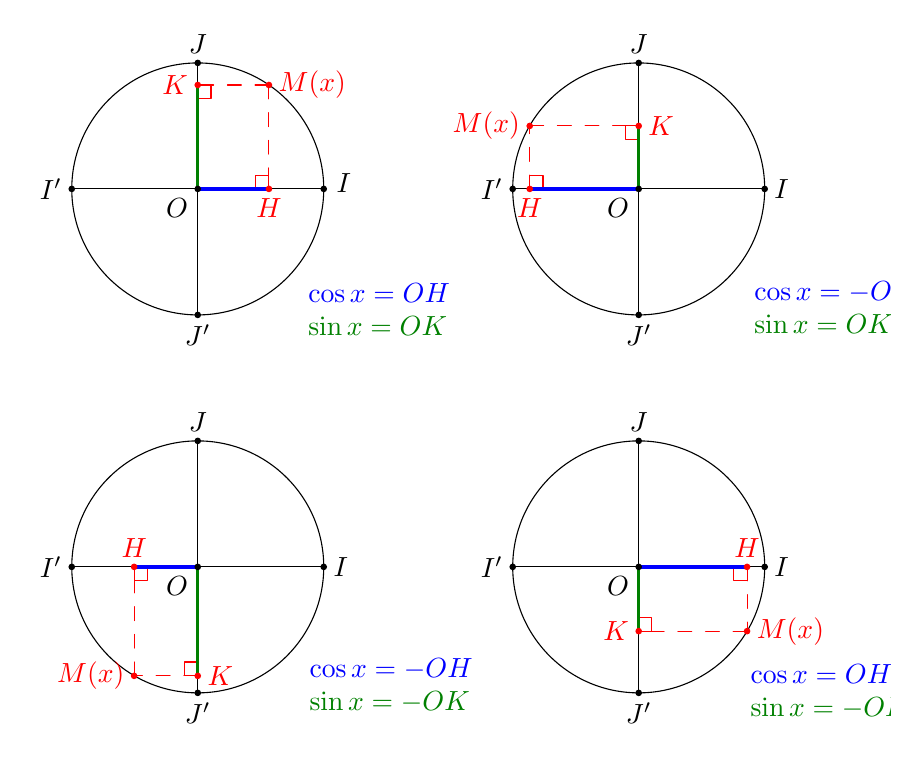
\begin{tikzpicture}[line cap=round,line join=round,>=triangle 45,x=1.0cm,y=1.0cm,scale=.8]
\clip(0.3,1) rectangle (14,12.56);
\draw[line width=0.4pt,color=red] (3,11.44) -- (3.21,11.44) -- (3.21,11.65) -- (3,11.65) -- cycle; 
\draw[line width=0.4pt,color=red] (4.13,10.21) -- (3.92,10.21) -- (3.92,10) -- (4.13,10) -- cycle; 
\draw[line width=0.4pt,color=red] (9.79,11) -- (9.79,10.79) -- (10,10.79) -- (10,11) -- cycle; 
\draw[line width=0.4pt,color=red] (8.48,10) -- (8.48,10.21) -- (8.27,10.21) -- (8.27,10) -- cycle; 
\draw[line width=0.4pt,color=red] (1.99,3.79) -- (2.2,3.79) -- (2.2,4) -- (1.99,4) -- cycle; 
\draw[line width=0.4pt,color=red] (3,2.49) -- (2.79,2.49) -- (2.79,2.27) -- (3,2.27) -- cycle; 
\draw[line width=0.4pt,color=red] (11.51,4) -- (11.51,3.79) -- (11.72,3.79) -- (11.72,4) -- cycle; 
\draw[line width=0.4pt,color=red] (10.21,2.98) -- (10.21,3.19) -- (10,3.19) -- (10,2.98) -- cycle; 
\draw(3,4) circle (2cm);
\draw(10,4) circle (2cm);
\draw(3,10) circle (2cm);
\draw(10,10) circle (2cm);
\draw (1,10)-- (5,10);
\draw (3,12)-- (3,8);
\draw [dash pattern=on 5pt off 5pt,color=red] (4.13,11.65)-- (3,11.65);
\draw [dash pattern=on 5pt off 5pt,color=red] (4.13,11.65)-- (4.13,10);
\draw (4.6,8.66) node[anchor=north west] {\parbox{2.12 cm}{${\color{blue}\cos x=OH}\\{\color{Green}\sin x = OK}$}};
\draw [line width=1.6pt,very thick,color=Green] (3,11.65)-- (3,10);
\draw [line width=1.6pt,very thick,color=blue] (3,10)-- (4.13,10);
\draw (10,12)-- (10,8);
\draw [dash pattern=on 5pt off 5pt,color=red] (8.27,10)-- (8.27,11);
\draw (12,10)-- (8,10);
\draw [dash pattern=on 5pt off 5pt,color=red] (8.27,11)-- (10,11);
\draw (10,6)-- (10,2);
\draw (8,4)-- (12,4);
\draw [dash pattern=on 5pt off 5pt,color=red] (11.72,4)-- (11.72,2.98);
\draw [dash pattern=on 5pt off 5pt,color=red] (11.72,2.98)-- (10,2.98);
\draw (1,4)-- (5,4);
\draw (3,6)-- (3,2);
\draw [dash pattern=on 5pt off 5pt,color=red] (3,2.27)-- (1.99,2.27);
\draw [dash pattern=on 5pt off 5pt,color=red] (1.99,2.27)-- (1.99,4);
\draw (0,0.24) node[anchor=north west] {\parbox{2.12 cm}{${\color{blue}\cos x=OH}\\{\color{Green}\sin x = OK}$}};
\draw (11.68,8.68) node[anchor=north west] {\parbox{2.2 cm}{${\color{blue}\cos x=-OH}\\{\color{Green}\sin x = OK}$}};
\draw (4.62,2.7) node[anchor=north west] {\parbox{2.2 cm}{${\color{blue}\cos x= -OH}\\{\color{Green}\sin x = -OK}$}};
\draw (11.62,2.6) node[anchor=north west] {\parbox{2.16 cm}{${\color{blue}\cos x=OH}\\{\color{Green}\sin x = -OK}$}};
\draw [very thick, color=blue] (8.27,10)-- (10,10);
\draw [very thick,color=Green] (10,10)-- (10,11);
\draw [very thick, color=blue] (3,4)-- (1.99,4);
\draw [very thick,color=Green] (3,4)-- (3,2.27);
\draw [very thick, color=blue] (10,4)-- (11.72,4);
\draw [very thick,color=Green] (10,4)-- (10,2.98);

\fill (3,4) circle (1.5pt);
\draw(3,4) node [below left]{$O$};
\fill (10,4) circle (1.5pt);
\draw(10,4) node [below left]{$O$};
\fill (3,10) circle (1.5pt);
\draw(3,10) node [below left]{$O$};
\fill (10,10) circle (1.5pt);
\draw(10,10) node [below left]{$O$};
\fill (1,10) circle (1.5pt);
\draw(1,10) node [left] {$I'$};
\fill (5,10) circle (1.5pt);
\draw(5.32,10.1) node {$I$};
\fill (3,12) circle (1.5pt);
\draw(3,12) node [above]{$J$};
\fill (3,8) circle (1.5pt);
\draw(3,8) node [below] {$J'$};
\fill [color=red] (4.13,11.65) circle (1.5pt);
\draw[color=red] (4.13,11.65) node [right] {$M(x)$};
\fill [color=red] (3,11.65) circle (1.5pt);
\draw[color=red] (3,11.65) node [left] {$K$};
\fill [color=red] (4.13,10) circle (1.5pt);
\draw[color=red] (4.13,10) node [below] {$H$};
\fill [color=red] (8.27,11) circle (1.5pt);
\draw[color=red] (8.27,11) node [left]{$M(x)$};
\fill [color=red] (1.99,2.27) circle (1.5pt);
\draw[color=red] (1.99,2.27) node [left]{$M(x)$};
\fill [color=red] (11.72,2.98) circle (1.5pt);
\draw[color=red] (11.72,2.98) node [right]{$M(x)$};
\fill [color=red] (10,11) circle (1.5pt);
\draw[color=red] (10,11) node [right]{$K$};
\fill [color=red] (8.27,10) circle (1.5pt);
\draw[color=red] (8.27,10) node [below]{$H$};
\fill [color=red] (10,2.98) circle (1.5pt);
\draw[color=red] (10,2.98) node [left]{$K$};
\fill [color=red] (11.72,4) circle (1.5pt);
\draw[color=red] (11.72,4) node [above]{$H$};
\fill [color=red] (3,2.27) circle (1.5pt);
\draw[color=red] (3,2.27) node [right]{$K$};
\fill [color=red] (1.99,4) circle (1.5pt);
\draw[color=red] (1.99,4) node [above]{$H$};
\fill (8,10) circle (1.5pt);
\draw(8,10)  node [left] {$I'$};
\fill (12,10) circle (1.5pt);
\draw(12,10) node [right] {$I$};
\fill (1,4) circle (1.5pt);
\draw(1,4)  node [left] {$I'$};
\fill (5,4) circle (1.5pt);
\draw(5,4) node [right] {$I$};
\fill (8,4) circle (1.5pt);
\draw(8,4)  node [left] {$I'$};
\fill (12,4) circle (1.5pt);
\draw(12,4) node [right] {$I$};
\fill (10,12) circle (1.5pt);
\draw(10,12) node [above] {$J$};
\fill (10,8) circle (1.5pt);
\draw(10,8) node [below] {$J'$};
\fill (10,6) circle (1.5pt);
\draw(10,6)  node [above] {$J$};
\fill (10,2) circle (1.5pt);
\draw(10,2) node [below] {$J'$};
\fill (3,6) circle (1.5pt);
\draw(3,6)  node [above] {$J$};
\fill (3,2) circle (1.5pt);
\draw(3,2) node [below] {$J'$};

\end{tikzpicture}


% ------•---- Les quatres cadrans --------------------------

Quatre quadrants.

\parbox{5cm}{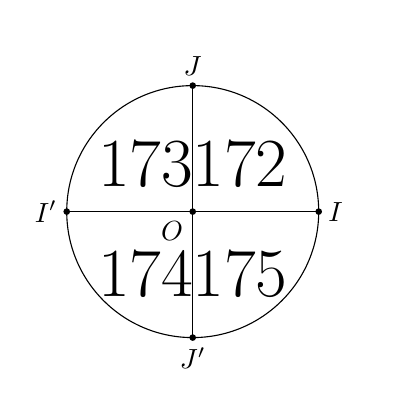
\begin{tikzpicture}[line cap=round,line join=round,>=triangle 45,x=1.0cm,y=1.0cm, scale=.8]
\clip (0.38,7.29) rectangle (6.04,12.92);
\draw (3,10) circle (2cm);
\draw (1,10)-- (5,10);
\draw (3,12)-- (3,8);
\draw (3.75,10.75)    node {\Huge \ding{172}};
\draw (2.25,10.75)       node {\Huge  \ding{173}};
\draw (2.25,9)     node {\Huge  \ding{174}};
\draw (3.75,9)  node {\Huge  \ding{175}};
\fill (3,10) circle (1.5pt);
\draw (3,10) node [below left]{$O$};
\fill (1,10) circle (1.5pt);
\draw (1,10) node [left] {$I'$};
\fill (5,10) circle (1.5pt);
\draw (5,10) node [right] {$I$};
\fill (3,12) circle (1.5pt);
\draw (3,12) node [above]{$J$};
\fill (3,8) circle (1.5pt);
\draw (3,8) node [below]{$J'$};
\end{tikzpicture}}
\parbox{10cm}{
   \ding{172} $\longrightarrow$\raisebox{-1ex}{$ \begin{array}{c}  
\cos (x) > 0 \\ 
\sin (x) >0 \\ 
   \end{array} 
        \qquad$}  
 \ding{173}
        $\longrightarrow$\raisebox{-1ex}{$\begin{array}{c}  
                 \cos (x) < 0 \\ 
                 \sin (x) > 0 \\ 
               \end{array}$}\\
               
               
\ding{174} 
    $\longrightarrow$\raisebox{-1ex}{$ \begin{array}{c}  
\cos (x) < 0 \\ 
\sin (x) < 0 \\ 
   \end{array} 
        \qquad$}  \ding{175}$\longrightarrow$\raisebox{-1ex}{ $\begin{array}{c}  
                 \cos (x) > 0 \\ 
                 \sin (x) < 0 \\ 
               \end{array}$}\\               
} \\
\renewcommand{\arraystretch }{1.75}
En particulier : 
\begin{quote}
{
\begin{tabular}{l@{$\;$}c@{$\qquad$}l@{$\;$}c}
$\bullet$  & $\cos 0 = 1 $ 
         & $\bullet$ & $\cos \dfrac{\pi}{2} = 0 $ \\  
          & $\sin 0 = 0 $ 
         &  & $\sin \dfrac{\pi}{2} = 1 $ \\  
& & & \\
$\bullet$  & $\cos \pi = -1 $ 
         & $\bullet$ & $\cos \dfrac{3\pi}{2} = 0 $ \\  
  & $\sin \pi = 0 $ 
         & & $\sin \dfrac{3\pi}{2} = -1 $ \\                             
\end{tabular}              
}
\end{quote}
\renewcommand{\arraystretch }{1}
\newpage 

Propriétés fondamentales pour $k \in \mathbb{Z}$  

\begin{quote}
\begin{tabular}{l@{$\,$}cc@{$\,$}l}
\ding{81} & Pour tout $x\in \Re$ & $\bullet$ & $-1
                       \leqslant \cos x  \leqslant 1 $ \\
          &          & $\bullet$ & $-1
                       \leqslant \sin x  \leqslant 1 $ \\
 & & & \\ 
 \ding{81} & Pour tout $x\in \Re$ & $\bullet$ 
                     & $ \cos (x+2k\pi) = \cos x $ \\
       &   & $\bullet$ & $ \sin x  (x+2k\pi) = \sin x $ \\
                        & & & \\ 
 \ding{81} & Pour tout $x\in \Re$ & $\bullet$ 
         & $ \cos^2 (x+2k\pi) + \sin^2 (x+2k\pi) = 1 $ \\

\end{tabular}\\

\bigskip

$(O, \overrightarrow{OI},  \overrightarrow{OJ})$ un repère orthonormal.\\

$M(\cos x, \sin x)$ dans $(O, \overrightarrow{OI},  \overrightarrow{OJ})$. \\

\begin{tabular}{r@{\,}l}
$ \cos^2 (x+2k\pi) + \sin^2 x $ &$= OH^2 + OK^2$\\
 &$= OH^2 + HM^2 $\\
 &$= OM^2$\\
 &$= 1 \qquad \qquad \text{ car }\; OM = 1 $\\ 
\end{tabular}\\

{\renewcommand{\arraystretch }{1.75}
\begin{tabular}{ll}
 
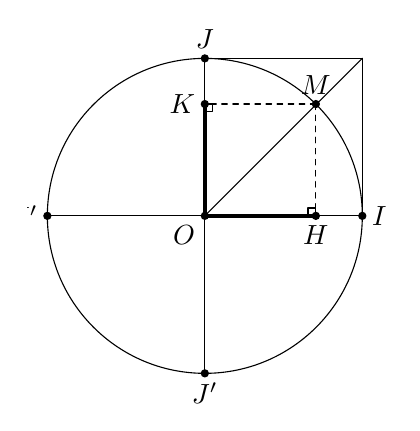
\begin{tikzpicture}[line cap=round,line join=round,>=triangle 45,x=1.0cm,y=1.0cm,scale=1]
\clip(-2.25,-2.38) rectangle (2.37,2.39);
\draw[line width=0.4pt] (0,1.32) -- (0.1,1.32) -- (0.1,1.42) -- (0,1.42) -- cycle; 
\draw[line width=0.4pt] (1.41,0.1) -- (1.31,0.1) -- (1.31,0) -- (1.41,0) -- cycle; 
\draw(0,0) circle (2cm);
\draw (-2,0)-- (2,0);
\draw (0,2)-- (0,-2);
\draw [dash pattern=on 2pt off 2pt] (1.41,1.42)-- (0,1.42);
\draw [dash pattern=on 2pt off 2pt] (1.41,1.42)-- (1.41,0);
\draw [line width=1.6pt] (0,1.42)-- (0,0);
\draw [line width=1.6pt] (0,0)-- (1.41,0);
\draw [line width=0.4pt] (0,2)-- (0,0);
\draw [line width=0.4pt] (0,0)-- (2,0);
\draw [line width=0.4pt] (2,0)-- (2,2);
\draw [line width=0.4pt] (2,2)-- (0,2);
\draw (0,0)-- (2,2);

\fill  (0,0) circle (1.5pt);
\draw(0,0) node [below left] {$O$};
\fill (-2,0) circle (1.5pt);
\draw(-2,0) node [left] {$I'$};
\fill (2,0) circle (1.5pt);
\draw(2,0) node [right] {$I$};
\fill (0,2) circle (1.5pt);
\draw(0,2) node [above] {$J$};
\fill (0,-2) circle (1.5pt);
\draw(0,-2) node [below] {$J'$};
\fill (1.41,1.42) circle (1.5pt);
\draw(1.41,1.42) node [above] {$M$};
\fill (0,1.42) circle (1.5pt);
\draw(0,1.42) node [left]{$K$};
\fill (1.41,0) circle (1.5pt);
\draw(1.41,0) node [below] {$H$};

\end{tikzpicture}


         &  \raisebox{27ex}{ \ding{81}}
            \raisebox{16.5ex}{              
         \parbox{.5\textwidth}{ 
        Cosinus et sinus de $\dfrac{\pi}{4}$ \\
        
        $ \begin{array}{r@{\;}l}
                 \cos^2 x + \sin^2 x              &= 1 \\
\cos^2 (\dfrac{\pi}{4}) + \sin^2 (\dfrac{\pi}{4}) &= 1 \\
                             2 sin^2 \dfrac{\pi}{4}      &= 1 \\ 
                         cos^2    \dfrac{\pi}{4} =     sin^2  \dfrac{\pi}{4} &= 
   \dfrac{1}{2} \quad \text { donc }= \dfrac{\sqrt{2}}{2} \text { ou } \cancel {-\dfrac{\sqrt{2}}{2}}\\  
        \end{array}$
         }}\\
\end{tabular}\\
\vspace*{-1cm}
\begin{center}
\fcolorbox{black}  {white}{
\hbox{
$\cos \dfrac{\pi}{4} = \dfrac{\sqrt{2}}{2} \quad \text{ et } \quad \sin \dfrac{\pi}{4} =  \dfrac{\sqrt{2}}{2} $ 
}}
\end{center}

\bigskip 

\begin{tabular}{ll}
 
% \definecolor{uuuuuu}{rgb}{0.27,0.27,0.27}
% \definecolor{qqffqq}{rgb}{0,1,0}
% \definecolor{ffqqqq}{rgb}{1,0,0}
% \definecolor{qqqqff}{rgb}{0,0,1}
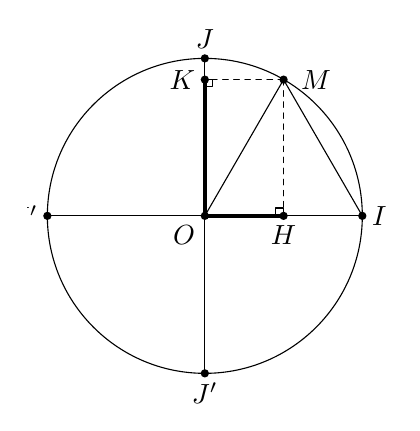
\begin{tikzpicture}[line cap=round,line join=round,>=triangle 45,x=1.0cm,y=1.0cm,scale=1]
\clip(-2.25,-2.38) rectangle (2.37,2.39);
\draw[line width=0.4pt] (0,1.64) -- (0.1,1.64) -- (0.1,1.73) -- (0,1.73) -- cycle; 
\draw[line width=0.4pt] (1,0.1) -- (0.9,0.1) -- (0.9,0) -- (1,0) -- cycle; 
\draw(0,0) circle (2cm);
\draw (-2,0)-- (2,0);
\draw (0,2)-- (0,-2);
\draw [dash pattern=on 2pt off 2pt] (1,1.73)-- (0,1.73);
\draw [dash pattern=on 2pt off 2pt] (1,1.73)-- (1,0);
\draw [line width=1.6pt] (0,1.73)-- (0,0);
\draw [line width=1.6pt] (0,0)-- (1,0);
\draw  (0,0)-- (2,0);
\draw  (2,0)-- (1,1.73);
\draw  (1,1.73)-- (0,0);

\fill  (0,0) circle (1.5pt);
\draw(0,0) node [below left] {$O$};
\fill (-2,0) circle (1.5pt);
\draw(-2,0) node [left] {$I'$};
\fill (2,0) circle (1.5pt);
\draw(2,0) node [right] {$I$};
\fill (0,2) circle (1.5pt);
\draw(0,2) node [above] {$J$};
\fill (0,-2) circle (1.5pt);
\draw(0,-2) node [below] {$J'$};
\fill  (1,1.73) circle (1.5pt);
\draw (1.1,1.73) node [right]{$M$};
\fill  (0,1.73) circle (1.5pt);
\draw (0,1.73) node [left] {$K$};
\fill  (1,0) circle (1.5pt);
\draw (1,0) node [below] {$H$};
\end{tikzpicture}

         &  \raisebox{31ex}{ \ding{81}}
            \raisebox{10ex}{              
         \parbox{.5\textwidth}{ 
        Cosinus et sinus de $\dfrac{\pi}{3}$ \\
        
        $ \begin{array}{r@{\;}l}
                 \cos^2 x + \sin^2 x              &= 1 \\
\cos^2 (\dfrac{\pi}{3}) + \sin^2 (\dfrac{\pi}{3}) &= 1 \\
                                       & \qquad \qquad 0H=\dfrac{1}{2} \\
                     \dfrac{1}{4} + \sin^2 (\dfrac{\pi}{3})    &= 1 \\
                       \sin^2 (\dfrac{\pi}{3}) &= 1 - \dfrac{1}{4} \\
                          \sin^2 (\dfrac{\pi}{3}) -\dfrac{3}{4}  &= 0 \\ 
 \left( \sin (\dfrac{\pi}{3} - \sqrt{\dfrac{3}{4}}\right)  \left( \sin (\dfrac{\pi}{3}) +\sqrt{\dfrac{3}{4}}\right) &= 0 \\       
                                   \sin (\dfrac{\pi}{3}) &= 
\dfrac{\sqrt{3}}{2} \text { ou } \cancel {-\dfrac{\sqrt{3}}{2}}\\  
        \end{array}$
         }}\\         
\end{tabular}\\
}
\renewcommand{\arraystretch }{1}
\begin{center}
\fcolorbox{black}  {white}{
\hbox{
$\cos \dfrac{\pi}{3} = \dfrac{1}{2} \quad \text{ et } \quad \sin \dfrac{\pi}{3} =  \dfrac{\sqrt{3}}{2} $ 
}}
\end{center}

\newpage

{\renewcommand{\arraystretch }{1.75}
\begin{tabular}{ll}

\begin{tikzpicture}[line cap=round,line join=round,>=triangle 45,x=1.0cm,y=1.0cm]
\clip(-2.4,-2.38) rectangle (2.8,2.39);
\draw(0,0) circle (2cm);
\draw (-2,0)-- (2,0);
\draw (0,2)-- (0,-2);
\draw [dash pattern=on 2pt off 2pt] (1.73,1)-- (0,1);
\draw [dash pattern=on 2pt off 2pt] (1.73,1)-- (1.73,0);
\draw [line width=1.6pt] (0,1)-- (0,0);
\draw [line width=1.6pt] (0,0)-- (1.73,0);
\draw [line width=2pt](0,0)-- (1.73,1);
\draw [line width=2pt](1.73,1)-- (0,2);
\draw [line width=2pt](0,0)-- (0,2);
\draw (0,2)-- (0,0);
\fill  (0,0) circle (1.5pt);
\draw(0,0) node [below left] {$O$};
\fill (-2,0) circle (1.5pt);
\draw(-2,0) node [left] {$I'$};
\fill (2,0) circle (1.5pt);
\draw(2,0) node [right] {$I$};
\fill (0,2) circle (1.5pt);
\draw(0,2) node [above] {$J$};
\fill (0,-2) circle (1.5pt);
\draw(0,-2) node [below] {$J'$};
\fill  (1.73,1) circle (1.5pt);
\draw (1.73,1) node [right] {$M(\dfrac{\pi}{6})$};
\fill  (0,1) circle (1.5pt);
\draw (0,1) node [left]{$K$};
\fill  (1.73,0) circle (1.5pt);
\draw (1.73,0) node [below] {$H$};
\end{tikzpicture}
         &  \raisebox{31ex}{ \ding{81}}
            \raisebox{10ex}{              
         \parbox{.5\textwidth}{ 
        Cosinus et sinus de $\dfrac{\pi}{6}$ \\
        
        $ \begin{array}{r@{\;}l}
                 \cos^2 x + \sin^2 x              &= 1 \\
\cos^2 (\dfrac{\pi}{6}) + \sin^2 (\dfrac{\pi}{6}) &= 1 \\
                                       & \qquad \qquad OK=\dfrac{1}{2} \\
                      \cos^2 (\dfrac{\pi}{6})  +\dfrac{1}{4}   &= 1 \\
                       \cos^2 (\dfrac{\pi}{6}) &= 1 - \dfrac{1}{4} \\
                          \cos^2 (\dfrac{\pi}{6}) -\dfrac{3}{4}  &= 0 \\ 
 \left( \cos^2 (\dfrac{\pi}{6}) - \sqrt{\dfrac{3}{4}}\right)  \left( \cos^2 (\dfrac{\pi}{6})) +\sqrt{\dfrac{3}{4}}\right) &= 0 \\       
                                   \cos (\dfrac{\pi}{6}) &= 
\dfrac{\sqrt{3}}{2} \text { ou } \cancel {-\dfrac{\sqrt{3}}{2}}\\  
        \end{array}$
         }}\\         
\end{tabular}\\
}
\renewcommand{\arraystretch }{1}
\begin{center}
\fcolorbox{black}  {white}{
\hbox{
$\cos \dfrac{\pi}{6} = \dfrac{\sqrt{3}}{2} \quad \text{ et } \quad \sin \dfrac{\pi}{6} =  \dfrac{1}{2} $ 
}}
\end{center}
\end{quote}

\vspace{2cm}

\underline{Récapitulation} : \\

\bigskip 

\hspace*{2cm}
{\renewcommand{\arraystretch }{2.3}
\begin{tabular}{|c||c|c|c|c|c|}
\hline
$x$ & $0$ & $\dfrac{\pi}{6}$ & $\dfrac{\pi}{4}$ & $\dfrac{\pi}{3}$ & $\dfrac{\pi}{2}$ \\
\hline
\hline
$\cos x$ & $1$ & $\dfrac{\sqrt{3}}{2}$ & $\dfrac{\sqrt{2}}{2}$ & $\dfrac{1}{2}$ & $0$ \\
\hline
$\sin x$ & $0$ & $\dfrac{1}{2}$ & $\dfrac{\sqrt{2}}{2}$ & $\dfrac{\sqrt{3}}{2}$ & $1$ \\
\hline
\end{tabular}
}

\vspace{2cm}


\centerline{
 \renewcommand{\arraystretch }{2.3}
\begin{tabular}{|c||c|c|c|c|c|c|c|c|c|c|c|c|c|c|c|c|}
\hline
$x$ & $0$ & $\dfrac{\pi}{6}$ & $\dfrac{\pi}{4}$ & $\dfrac{\pi}{3}$ & $\dfrac{\pi}{2}$ & $\dfrac{2\pi}{3}$ & $\dfrac{3\pi}{4}$ & $\dfrac{5\pi}{6}$ & $\pi$ & $\dfrac{7\pi}{6}$ & $\dfrac{5\pi}{4}$ & $\dfrac{4\pi}{3}$ & $\dfrac{3\pi}{2}$ & $\dfrac{5\pi}{3}$ & $\dfrac{7\pi}{4}$ & $\dfrac{11\pi}{6}$ \\
\hline
\hline
$\cos x$ & $1$ & $\dfrac{\sqrt{3}}{2}$ & $\dfrac{\sqrt{2}}{2}$ & $\dfrac{1}{2}$ & $0$
         & $-\dfrac{1}{2}$ & $-\dfrac{\sqrt{2}}{2}$ & $- \dfrac{\sqrt{3}}{2}$ & $-1$ 
         & $-\dfrac{\sqrt{3}}{2}$ & $-\dfrac{\sqrt{2}}{2}$ & $-\dfrac{1}{2}$ & $0$ 
         & $\dfrac{1}{2}$ & $\dfrac{\sqrt{2}}{2}$ & $\dfrac{\sqrt{3}}{2}$\\
\hline
$\sin x$ & $0$ &  $\dfrac{1}{2}$ & $\dfrac{\sqrt{2}}{2}$ & $\dfrac{\sqrt{3}}{2}$ & $1$
         & $\dfrac{\sqrt{3}}{2}$ & $\dfrac{\sqrt{2}}{2}$ & $\dfrac{1}{2}$ & $0$
         & $-\dfrac{1}{2}$ & $-\dfrac{\sqrt{2}}{2}$ & $- \dfrac{\sqrt{3}}{2}$ & $-1$ 
         & $-\dfrac{\sqrt{3}}{2}$ & $-\dfrac{\sqrt{2}}{2}$ & $-\dfrac{1}{2}$\\
\hline
\end{tabular}
}



\newpage

\subsection*{Formules de transposition}

\definecolor{uuuuuu}{rgb}{0.27,0.27,0.27}
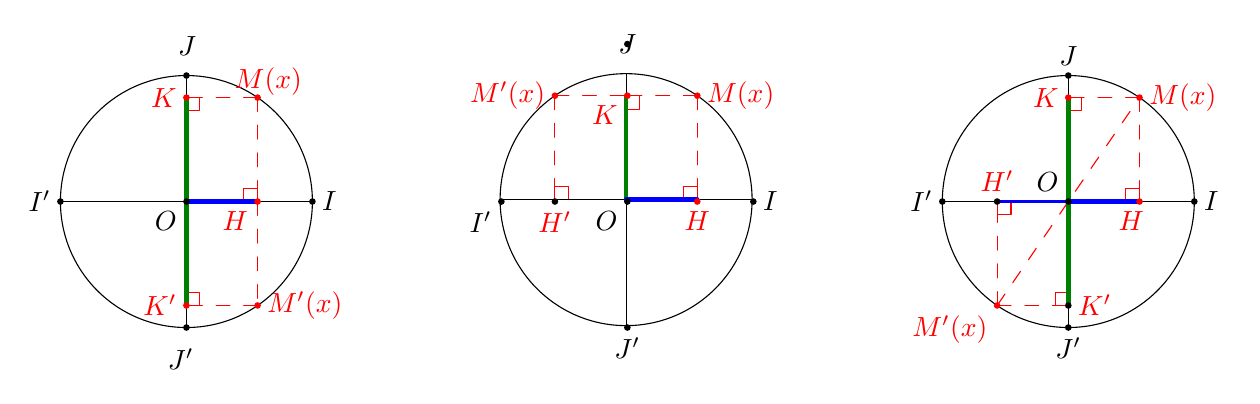
\begin{tikzpicture}[line cap=round,line join=round,>=triangle 45,x=1.0cm,y=1.0cm,scale=.8]
\clip(-2.52,-2.76) rectangle (16.6,2.76);
\draw[line width=0.4pt,color=red] (0,1.44) -- (0.21,1.44) -- (0.21,1.65) -- (0,1.65) -- cycle; 
\draw[line width=0.4pt,color=red] (1.13,0.21) -- (0.91,0.21) -- (0.91,0) -- (1.13,0) -- cycle; 
\draw[line width=0.4pt,color=red] (0.21,-1.65) -- (0.21,-1.44) -- (0,-1.44) -- (0,-1.65) -- cycle; 
\draw[line width=0.4pt,color=red] (6.98,1.46) -- (7.19,1.46) -- (7.19,1.68) -- (6.98,1.68) -- cycle; 
\draw[line width=0.4pt,color=red] (8.11,0.24) -- (7.89,0.24) -- (7.89,0.03) -- (8.11,0.03) -- cycle; 
\draw[line width=0.4pt,color=red] (14,1.44) -- (14.21,1.44) -- (14.21,1.65) -- (14,1.65) -- cycle; 
\draw[line width=0.4pt,color=red] (15.13,0.21) -- (14.91,0.21) -- (14.91,0) -- (15.13,0) -- cycle; 
\draw[line width=0.4pt,color=red] (6.07,0.03) -- (6.07,0.24) -- (5.85,0.24) -- (5.85,0.03) -- cycle; 
\draw[line width=0.4pt,color=red] (12.87,-0.21) -- (13.09,-0.21) -- (13.09,0) -- (12.87,0) -- cycle; 
\draw[line width=0.4pt,color=red] (14,-1.44) -- (13.79,-1.44) -- (13.79,-1.65) -- (14,-1.65) -- cycle; 
\draw(0,0) circle (2cm);
\draw (-2,0)-- (2,0);
\draw (0,2)-- (0,-2);
\draw [dash pattern=on 5pt off 5pt,color=red] (1.13,1.65)-- (0,1.65);
\draw [dash pattern=on 5pt off 5pt,color=red] (1.13,1.65)-- (1.13,0);
\draw [line width=1.6pt,color=Green] (0,1.65)-- (0,0);
\draw [line width=1.6pt,color=blue] (0,0)-- (1.13,0);
\draw [dash pattern=on 5pt off 5pt,color=red] (1.13,0)-- (1.13,-1.65);
\draw [dash pattern=on 5pt off 5pt,color=red] (1.13,-1.65)-- (0,-1.65);
\draw [line width=1.6pt,color=Green] (0,-1.65)-- (0,0);
\draw(6.98,0.03) circle (2cm);
\draw (4.98,0.03)-- (8.98,0.03);
\draw (6.98,2.03)-- (6.98,-1.97);
\draw [dash pattern=on 5pt off 5pt,color=red] (8.11,1.68)-- (6.98,1.68);
\draw [dash pattern=on 5pt off 5pt,color=red] (8.11,1.68)-- (8.11,0.03);
\draw [line width=1.6pt,color=Green] (6.98,1.68)-- (6.98,0.03);
\draw [line width=1.6pt,color=blue] (6.98,0.03)-- (8.11,0.03);
\draw(14,0) circle (2cm);
\draw (12,0)-- (16,0);
\draw (14,2)-- (14,-2);
\draw [dash pattern=on 5pt off 5pt,color=red] (15.13,1.65)-- (14,1.65);
\draw [dash pattern=on 5pt off 5pt,color=red] (15.13,1.65)-- (15.13,0);
\draw [line width=1.6pt,color=Green] (14,1.65)-- (14,0);
\draw [line width=1.6pt,color=blue] (14,0)-- (15.13,0);
\draw [dash pattern=on 5pt off 5pt,color=red] (5.85,1.68)-- (6.98,1.68);
\draw [dash pattern=on 5pt off 5pt,color=red] (5.85,1.68)-- (5.85,0.03);
\draw [dash pattern=on 5pt off 5pt,color=red] (12.87,-1.65)-- (15.13,1.65);
\draw [dash pattern=on 5pt off 5pt,color=red] (12.87,-1.65)-- (14,-1.65);
\draw [dash pattern=on 5pt off 5pt,color=red] (12.87,-1.65)-- (12.87,0);
\draw [line width=1.6pt,color=Green] (14,0)-- (14,-1.65);
\draw [line width=1.2pt,color=blue] (14,0)-- (12.87,0);
\fill (0,0) circle (1.5pt);
\draw(0,0) node [below left] {$O$};
\fill (-2,0) circle (1.5pt);
\draw(-2,0) node [left] {$I'$};
\fill (2,0) circle (1.5pt);
\draw(2,0) node [right] {$I$};
\fill (0,2) circle (1.5pt);
\draw(0.01,2.47) node {$J$};
\fill (0,-2) circle (1.5pt);
\draw(-0.09,-2.18) node [below] {$J'$};
\fill [color=red] (1.13,1.65) circle (1.5pt);
\draw[color=red] (1.3,1.91) node {$M(x)$};
\fill [color=red] (0,1.65) circle (1.5pt);
\draw[color=red] (0,1.65) node [left]{$K$};
\fill [color=red] (1.13,0) circle (1.5pt);
\draw[color=red] (1.13,0) node [below left]{$H$};
\fill [color=red] (1.13,-1.65) circle (1.5pt);
\draw[color=red] (1.13,-1.65) node [right]{$M'(x)$};
\fill [color=red] (0,-1.65) circle (1.5pt);
\draw[color=red] (0,-1.65) node [left] {$K'$};
\fill (7,0) circle (1.5pt);
\draw(7,0) node [below left]{$O$};
\fill (5,0) circle (1.5pt);
\draw(5,0) node[below left] {$I'$};
\fill (9,0) circle (1.5pt);
\draw(9,0) node [right] {$I$};
\fill (7,2.5) circle (1.5pt);
\draw(7,2.5) node {$J$};
\fill (7,-2) circle (1.5pt);
\draw(7,-2) node [below] {$J'$};
\fill [color=red] (8.11,1.68) circle (1.5pt);
\draw[color=red] (8.11,1.68) node [right]{$M(x)$};
\fill [color=red] (7,1.68) circle (1.5pt);
\draw[color=red] (7,1.68) node [below left] {$K$};
\fill [color=red] (8.11,0) circle (1.5pt);
\draw[color=red] (8.11,0) node [below]{$H$};
\fill (14,0) circle (1.5pt);
\draw(14,0) node [above left]{$O$};
\fill (12,0) circle (1.5pt);
\draw(12,0) node [left]{$I'$};
\fill (16,0) circle (1.5pt);
\draw(16,0) node [right] {$I$};
\fill (14,2) circle (1.5pt);
\draw(14,2) node [above]{$J$};
\fill (14,-2) circle (1.5pt);
\draw(14,-2) node [below]{$J'$};
\fill [color=red] (15.13,1.65) circle (1.5pt);
\draw[color=red] (15.13,1.65) node [right]{$M(x)$};
\fill [color=red] (14,1.65) circle (1.5pt);
\draw[color=red] (14,1.65) node [left]{$K$};
\fill [color=red] (15.13,0) circle (1.5pt);
\draw[color=red] (15,0) node [below]{$H$};
\fill [color=red] (5.85,1.68) circle (1.5pt);
\draw[color=red] (5.85,1.68) node [left]{$M'(x)$};
\fill (5.85,0) circle (1.5pt);
\draw [color=red] (5.85,0) node [below] {$H'$};
\fill [color=red] (12.87,-1.65) circle (1.5pt);
\draw[color=red] (12.87,-1.65) node [below left]{$M'(x)$};
\fill (12.87,0) circle (1.5pt);
\draw [color=red] (12.87,0) node [above]{$H'$};
\fill (14,-1.65) circle (1.5pt);
\draw [color=red](14,-1.65) node [right] {$K'$};
\end{tikzpicture}


\bigskip 

\centerline{
\begin{tabular}{c@{$\,$}l@{\hspace{3cm}}c@{$\,$}l@{\hspace{3cm}}c@{$\,$}l}
% $\bullet$ & $M'(x) \text{ image de } x $ & 
%      $\bullet$ & $M'(\pi - x) \text{ image de } \pi - x $& 
%           $\bullet$ & $M'(\pi + x) \text{ image de } \pi + x $ \\
&$\cos (-x) = \cos (x) $& &$\cos (\pi -x) = -\cos (x)$&&$\cos (\pi+x) = -\cos (x)$\\
&$\sin(-x) = -\sin (x) $& &$\sin (\pi -x) = \sin (x)$&&$\sin (\pi+x) = \sin (x)$\\
\end{tabular}
}

\centerline{
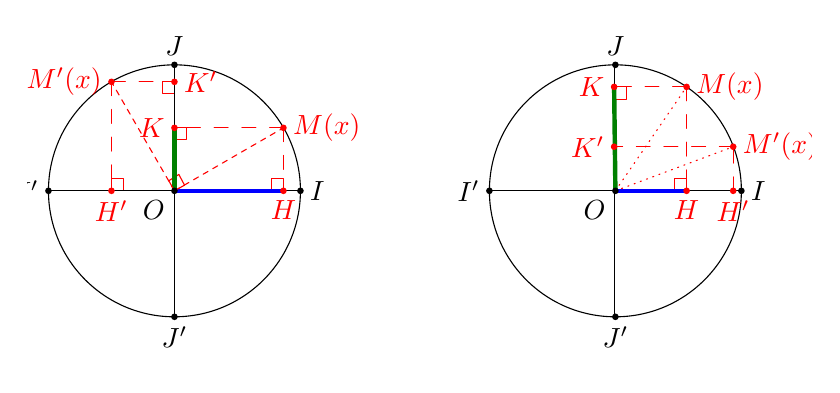
\begin{tikzpicture}[line cap=round,line join=round,>=triangle 45,x=1.0cm,y=1.0cm, scale=.8]
\clip(-2.33,-2.76) rectangle (10.12,2.59);
\draw[line width=0.4pt,color=red] (0,0.81) -- (0.19,0.81) -- (0.19,1) -- (0,1) -- cycle; 
\draw[line width=0.4pt,color=red] (1.73,0.19) -- (1.54,0.19) -- (1.54,0) -- (1.73,0) -- cycle; 
\draw[line width=0.4pt,color=red] (6.98,1.65) -- (7.18,1.65) -- (7.18,1.45) -- (6.98,1.45) -- cycle; 
\draw[line width=0.4pt,color=red] (8.13,0.19) -- (7.94,0.19) -- (7.94,0) -- (8.13,0) -- cycle; 
\draw[line width=0.4pt,color=red] (0.16,0.09) -- (0.07,0.26) -- (-0.09,0.16) -- (0,0) -- cycle; 
\draw[line width=0.4pt,color=red] (-0.19,1.73) -- (-0.19,1.54) -- (0,1.54) -- (0,1.73) -- cycle; 
\draw[line width=0.4pt,color=red] (-0.81,0) -- (-0.81,0.19) -- (-1,0.19) -- (-1,0) -- cycle; 
\draw(0,0) circle (2cm);
\draw (-2,0)-- (2,0);
\draw (0,2)-- (0,-2);
\draw [dash pattern=on 5pt off 5pt,color=red] (1.73,1)-- (0,1);
\draw [dash pattern=on 5pt off 5pt,color=red] (1.73,1)-- (1.73,0);
\draw [line width=1.6pt,color=Green] (0,1)-- (0,0);
\draw [line width=1.6pt,color=blue] (0,0)-- (1.73,0);
\draw(7,0) circle (2cm);
\draw (5,0)-- (9,0);
\draw (6.98,2.03)-- (6.98,-1.97);
\draw [dash pattern=on 5pt off 5pt,color=red] (8.13,1.65)-- (6.98,1.65);
\draw [dash pattern=on 5pt off 5pt,color=red] (8.13,1.65)-- (8.13,0);
\draw [line width=1.6pt,color=Green] (6.98,1.65)-- (7,0);
\draw [line width=1.6pt,color=blue] (7,0)-- (8.13,0);
\draw [dash pattern=on 2pt off 2pt,color=red] (0,0)-- (-1,1.73);
\draw [dash pattern=on 2pt off 2pt,color=red] (0,0)-- (1.73,1);
\draw [dash pattern=on 5pt off 5pt,color=red] (-1,1.73)-- (0,1.73);
\draw [dash pattern=on 5pt off 5pt,color=red] (-1,1.73)-- (-1,0);
\draw [dotted,color=red] (7,0)-- (8.87,0.7);
\draw [dotted,color=red] (7,0)-- (8.13,1.65);
\draw [dash pattern=on 5pt off 5pt,color=red] (8.87,0)-- (8.87,0.7);
\draw [dash pattern=on 5pt off 5pt,color=red] (8.87,0.7)-- (6.98,0.7);
\fill  (0,0) circle (1.5pt);
\draw (0,0) node [below left]{$O$};
\fill  (-2,0) circle (1.5pt);
\draw (-2,0) node [left]{$I'$};
\fill  (2,0) circle (1.5pt);
\draw (2,0) node [right] {$I$};
\fill  (0,2) circle (1.5pt);
\draw (0,2) node [above] {$J$};
\fill  (0,-2) circle (1.5pt);
\draw (0,-2) node [below] {$J'$};
\fill [color=red] (1.73,1) circle (1.5pt);
\draw[color=red] (1.73,1) node [right] {$M(x)$};
\fill [color=red] (0,1) circle (1.5pt);
\draw[color=red] (0,1) node [left] {$K$};
\fill [color=red] (1.73,0) circle (1.5pt);
\draw[color=red] (1.73,0) node [below] {$H$};
\fill  (7,0) circle (1.5pt);
\draw (7,0) node [below left]{$O$};
\fill  (5,0) circle (1.5pt);
\draw (5,0) node [left] {$I'$};
\fill  (9,0) circle (1.5pt);
\draw (9,0) node [right] {$I$};
\fill  (7,2) circle (1.5pt);
\draw (7,2) node [above] {$J$};
\fill  (7,-2) circle (1.5pt);
\draw (7,-2) node [below] {$J'$};
\fill [color=red] (8.13,1.65) circle (1.5pt);
\draw[color=red] (8.13,1.65) node [right]{$M(x)$};
\fill [color=red] (6.98,1.65) circle (1.5pt);
\draw[color=red] (6.98,1.65) node [left] {$K$};
\fill [color=red] (8.13,0) circle (1.5pt);
\draw[color=red] (8.13,0) node [below] {$H$};
\fill [color=red] (-1,1.73) circle (1.5pt);
\draw[color=red] (-1,1.73) node [left] {$M'(x)$};
\fill [color=red] (0,1.73) circle (1.5pt);
\draw[color=red] (0,1.73) node [right] {$K'$};
\fill [color=red] (-1,0) circle (1.5pt);
\draw[color=red] (-1,0) node [below]{$H'$};
\fill [color=red] (8.87,0.7) circle (1.5pt);
\draw[color=red] (8.87,0.7) node [right] {$M'(x)$};
\fill [color=red] (6.98,0.7) circle (1.5pt);
\draw[color=red] (6.98,0.7) node [left] {$K'$};
\fill [color=red] (8.87,0) circle (1.5pt);
\draw[color=red] (8.87,0) node [below] {$H'$};
\end{tikzpicture}
}

\centerline{\renewcommand{\arraystretch }{2}
\begin{tabular}{c@{$\,$}l@{\hspace{2.5cm}}%
                           c@{$\,$}l}
% $\bullet$ & $M'\left( x+\dfrac{\pi}{2} \right) \text{ est l'image ddu réel  } x $ & 
%      $\bullet$ & $M'\left(\dfrac{\pi}{2} - x\right) \text{ image de } x $ \\
           &$\cos \left(x+\dfrac{\pi}{2}\right) = -\sin (x) $& 
               &$\cos \left(\dfrac{\pi}{2} -x\right) = \sin (x)$\\
          &$\sin \left(x+\dfrac{\pi}{2}\right) = \cos (x) $& 
            &$\sin \left(\dfrac{\pi}{2} -x\right) = \cos (x)$\\
\end{tabular}}

\vspace*{.3cm}

Un superbe exercice : 

Soit $x\in \mathbb{R}$, simplifier : 

\begin{enumerate}

\item \raisebox{-2.8ex}{\renewcommand{\arraystretch }{1}
\begin{tabular}{r@{}l}
$A$&$=\cos x +\cos \left(\dfrac{\pi}{2}-x\right) +\cos \left(x +\dfrac{\pi}{2}\right)+\cos (\pi -x) $\\ 
   &$=\cos x + \sin x - \sin x - \cos x $ \\
   & $= 0$ \\
\end{tabular}}

\item \raisebox{-7ex}{\renewcommand{\arraystretch }{1.6}
\begin{tabular}{r@{$\,$}l}
$A'$&$=\cos \left(\dfrac{\pi}{8}\right) +\cos \left(\dfrac{3\pi}{8}\right)+ \cos \left(\dfrac{5\pi}{8}\right) +\cos \left(\dfrac{7\pi}{8}\right)$\\ 
    &$=\cos \left(\dfrac{\pi}{8}\right) +\cos \left(\dfrac{\pi}{2}-\dfrac{\pi}{8}\right)+ \cos \left(\dfrac{\pi}{2}+\dfrac{\pi}{8}\right) +\cos \left(\pi - \dfrac{\pi}{8}\right)$\\ 
   &$=\cos \dfrac{\pi}{8}+ \sin \dfrac{\pi}{8} -  \sin \dfrac{\pi}{8} - \cos \dfrac{\pi}{8}$  \\
   & $=0$ \\
\end{tabular}}

\item \raisebox{-3ex}{\renewcommand{\arraystretch }{1}
\begin{tabular}{r@{$\,$}l}
 $B$ & $=\sin^2 x 
         + \sin^2\left(\dfrac{\pi}{2} - x\right) 
         + \sin^2\left(x +\dfrac{\pi}{2}\right)
         +\sin^2 (\pi - x) $\\ 
   & $=\sin^2 x + \cos^2 x + \cos^2 x + \sin^2 x $  \\
   & $= 1 + 1 = 2 $ \\
\end{tabular}}

\item \raisebox{-4.5ex}{\renewcommand{\arraystretch }{1.6}
\begin{tabular}{r@{$\,$}l}
$B'$&$= \sin^2 \left(\dfrac{\pi}{8}\right) 
      + \sin^2 \left(\dfrac{\pi}{2} - \dfrac{\pi}{8}\right)) 
      + \sin^2 \left(\dfrac{\pi}{2}+\dfrac{\pi}{8}\right)) +  \sin^2 (\pi - \dfrac{\pi}{8}) $\\ 
    &$=\sin^2 \left(\dfrac{\pi}{8}\right) 
       + \cos^2 \left(\dfrac{\pi}{8}\right) 
       + \cos^2 \left(\dfrac{\pi}{8}\right) 
       + \sin^2 \left(\dfrac{\pi}{8}\right) $  \\
   & $= 1 + 1 = 2 $ \\
\end{tabular}}

\end{enumerate}

\samepage

\newpage 

\renewcommand{\arraystretch }{1}

\subsection{Représentations graphiques}

\subsubsection{Représentation graphique de la fonction sinus}

\begin{tabular}{rl}
$\sin\quad : $ & $\mathbb{R} \longrightarrow \mathbb{R} $ \\
               &  $x \longmapsto \sin x $ \\
               & \\
               & $ {\Large \mathcal{D}_{\sin}} = \mathbb{R} $ \\
\end{tabular}\\

\input{Sinusoide.tex}

\bigskip 

La fonction sinus est périodique de période $2\pi$. \\

La fonction est dite \underline{sinusoïde}. 


\bigskip 

\subsubsection{Représentation graphique de la fonction cosinus}

\begin{tabular}{rl}
$\cos\quad : $ & $\mathbb{R} \longrightarrow \mathbb{R} $ \\
               &  $x \longmapsto \cos x $ \\
               & \\
               & $ {\Large \mathcal{D}_{\cos}} = \mathbb{R} $ \\
\end{tabular}\\

% \definecolor{ttzzqq}{rgb}{0.2,0.6,0} % Vert agreable
% \definecolor{qqzzqq}{rgb}{0,0.6,0}   % Vert agreable
% \definecolor{ffefdv}{rgb}{1,0.94,0.84} % AntiqueWhite pour grid
\begin{tikzpicture}[line cap=round,line join=round,>=triangle 45,x=1.0cm,y=1.0cm,scale=.8]
% \draw [color=AntiqueWhite,, xstep=0.1cm,ystep=0.1cm] (-7.1,-1.54) grid (13.29,2.53);
\draw[->,color=black] (-7.1,0) -- (13.29,0);
\foreach \x in {-6,-4,-2,2,4,6,8,10,12}
\draw[shift={(\x,0)},color=black] (0pt,2pt) -- (0pt,-2pt);
\draw[->,color=black] (0,-1.54) -- (0,2.53);
\foreach \y in {-1,1,2}
\draw[shift={(0,\y)},color=black] (2pt,0pt) -- (-2pt,0pt);
\clip(-7.1,-1.54) rectangle (13.29,2.53);
\draw[color=Green, smooth,samples=100,domain=-7.097377544417069:13.285348399587015] plot(\x,{cos(((\x))*180/pi)});

% \draw (-6.28,1.5)-- (-6.28,-2);
% \draw (0,2.39)-- (0,-2.27);
% \draw (12.57,1.5)-- (12.57,-2);
% \draw (6.28,2)-- (6.28,-2);


% Délimite les périodes 
\draw (-6.28,2)-- (-6.28,-2);
% \draw (0,2.39)-- (0,-2.27);
\draw (12.57,2)-- (12.57,-2);
\draw (6.28,2)-- (6.28,-2);

\draw (0,2) -- node[below, midway] {Période $2\pi$}  (6.28,2);
% \draw (1.53,1.78) node] {...};
\begin{tiny}
\draw  (1.05,0)-- ++(-1.0pt,0 pt) -- ++(2.0pt,0 pt) ++(-1.0pt,-1.0pt) -- ++(0 pt,2.0pt);
\draw (pi/3,0) node [below]{$\dfrac{\pi}{3}$};
\draw  (1.57,0)-- ++(-1.0pt,0 pt) -- ++(2.0pt,0 pt) ++(-1.0pt,-1.0pt) -- ++(0 pt,2.0pt);
\draw (pi/2,0 ) node [below] {$\dfrac{\pi}{2}$};
\draw  (3.67,0)-- ++(-1.0pt,0 pt) -- ++(2.0pt,0 pt) ++(-1.0pt,-1.0pt) -- ++(0 pt,2.0pt);
\draw (2*pi/3,0) node [below]{$\dfrac{2\pi}{3}$};
\draw  (4.71,0)-- ++(-1.0pt,0 pt) -- ++(2.0pt,0 pt) ++(-1.0pt,-1.0pt) -- ++(0 pt,2.0pt);
\draw (3*pi/2,0) node [below] {$\dfrac{3\pi}{2}$};
\draw  (5.76,0)-- ++(-1.0pt,0 pt) -- ++(2.0pt,0 pt) ++(-1.0pt,-1.0pt) -- ++(0 pt,2.0pt);
\draw (5*pi/6,0) node [below] {$\dfrac{5\pi}{6}$};
\draw [color=Green] (6.28,0)-- ++(-1.0pt,-1.0pt) -- ++(2.0pt,2.0pt) ++(-2.0pt,0) -- ++(2.0pt,-2.0pt);
\draw  (2.62,0)-- ++(-1.0pt,0 pt) -- ++(2.0pt,0 pt) ++(-1.0pt,-1.0pt) -- ++(0 pt,2.0pt);
\draw (11*pi/6,0) node [above]{$\dfrac{11\pi}{6}$};
\draw (7*pi/6,0) node [above]{$\dfrac{7\pi}{6}$};
\draw  (0.57,0)-- ++(-1.0pt,0 pt) -- ++(2.0pt,0 pt) ++(-1.0pt,-1.0pt) -- ++(0 pt,2.0pt);
\draw (pi/6,0) node [below] {$\dfrac{\pi}{6}$};
\draw (0,0.5) node [left] {$\dfrac{1}{2}$};
\draw  (0,-0.5)-- ++(-1.0pt,0 pt) -- ++(2.0pt,0 pt) ++(-1.0pt,-1.0pt) -- ++(0 pt,2.0pt);
\draw (0,-0.5) node [left]{$-\dfrac{1}{2}$};
\end{tiny}
\begin{scriptsize}
\draw (pi,0) node [above]{$\pi$};
\draw (2*pi,0) node [below right]{$2\pi$};
\draw (0,1) node[right] {$1$};
\draw  (0,-1)-- ++(-1.0pt,0 pt) -- ++(2.0pt,0 pt) ++(-1.0pt,-1.0pt) -- ++(0 pt,2.0pt);
\draw (0,-1) node [left]{$-1$};
\end{scriptsize}
\fill [color=black,shift={(0.1,2)},rotate=90] (0,0) ++(0 pt,2.25pt) -- ++(1.95pt,-3.375pt)--++(-3.9pt,0 pt) -- ++(1.95pt,3.375pt);
\fill [color=black,shift={(6.18,2)},rotate=270] (0,0) ++(0 pt,2.25pt) -- ++(1.95pt,-3.375pt)--++(-3.9pt,0 pt) -- ++(1.95pt,3.375pt);


\draw [color=Green] (0.52-pi/2,0.5)-- ++(-1.0pt,-1.0pt) -- ++(2.0pt,2.0pt) ++(-2.0pt,0) -- ++(2.0pt,-2.0pt);
\draw [color=Green] (-6.28-pi/2,0)-- ++(-1.0pt,-1.0pt) -- ++(2.0pt,2.0pt) ++(-2.0pt,0) -- ++(2.0pt,-2.0pt);
\draw [color=Green] (-5.76-pi/2,0.5)-- ++(-1.0pt,-1.0pt) -- ++(2.0pt,2.0pt) ++(-2.0pt,0) -- ++(2.0pt,-2.0pt);
\draw [color=Green] (-4.71-pi/2,1)-- ++(-1.0pt,-1.0pt) -- ++(2.0pt,2.0pt) ++(-2.0pt,0) -- ++(2.0pt,-2.0pt);
\draw [color=Green] (-3.67-pi/2,0.5)-- ++(-1.0pt,-1.0pt) -- ++(2.0pt,2.0pt) ++(-2.0pt,0) -- ++(2.0pt,-2.0pt);
\draw [color=Green] (-2.62-pi/2,-0.5)-- ++(-1.0pt,-1.0pt) -- ++(2.0pt,2.0pt) ++(-2.0pt,0) -- ++(2.0pt,-2.0pt);
\draw [color=Green] (-3.14-pi/2,0)-- ++(-1.0pt,-1.0pt) -- ++(2.0pt,2.0pt) ++(-2.0pt,0) -- ++(2.0pt,-2.0pt);
\draw [color=Green] (-1.57-pi/2,-1)-- ++(-1.0pt,-1.0pt) -- ++(2.0pt,2.0pt) ++(-2.0pt,0) -- ++(2.0pt,-2.0pt);
\draw [color=Green] (-0.52-pi/2,-0.5)-- ++(-1.0pt,-1.0pt) -- ++(2.0pt,2.0pt) ++(-2.0pt,0) -- ++(2.0pt,-2.0pt);
\draw [color=Green] (1.05-pi/2,0.87)-- ++(-1.0pt,-1.0pt) -- ++(2.0pt,2.0pt) ++(-2.0pt,0) -- ++(2.0pt,-2.0pt);
\draw [color=Green] (1.57-pi/2,1)-- ++(-1.0pt,-1.0pt) -- ++(2.0pt,2.0pt) ++(-2.0pt,0) -- ++(2.0pt,-2.0pt);
\draw [color=Green] (2.09-pi/2,0.87)-- ++(-1.0pt,-1.0pt) -- ++(2.0pt,2.0pt) ++(-2.0pt,0) -- ++(2.0pt,-2.0pt);
\draw [color=Green] (2.62-pi/2,0.5)-- ++(-1.0pt,-1.0pt) -- ++(2.0pt,2.0pt) ++(-2.0pt,0) -- ++(2.0pt,-2.0pt);
\draw [color=Green] (3.14-pi/2,0)-- ++(-1.0pt,-1.0pt) -- ++(2.0pt,2.0pt) ++(-2.0pt,0) -- ++(2.0pt,-2.0pt);
\draw [color=Green] (3.67-pi/2,-0.5)-- ++(-1.0pt,-1.0pt) -- ++(2.0pt,2.0pt) ++(-2.0pt,0) -- ++(2.0pt,-2.0pt);
\draw [color=Green] (4.71-pi/2,-1)-- ++(-1.0pt,-1.0pt) -- ++(2.0pt,2.0pt) ++(-2.0pt,0) -- ++(2.0pt,-2.0pt);
\draw [color=Green] (5.76-pi/2,-0.5)-- ++(-1.0pt,-1.0pt) -- ++(2.0pt,2.0pt) ++(-2.0pt,0) -- ++(2.0pt,-2.0pt);
\draw  (0,0.5)-- ++(-1.0pt,0 pt) -- ++(2.0pt,0 pt) ++(-1.0pt,-1.0pt) -- ++(0 pt,2.0pt);

\begin{pgfonlayer}{background}  
% Attention l'ordre de ces lignes est important 
% Ne pas le modifier   
\draw[step=1mm,ultra thin,AntiqueWhite!10](-7,-2)  grid (14,2.6);
\draw[step=5mm,very thin,AntiqueWhite!30] (-7,-2)  grid (14,2.6);
\draw[step=1cm,very thin,AntiqueWhite!50] (-7,-2)  grid (14,2.6);
\draw[step=5cm,thin,AntiqueWhite]         (-7,-2)  grid (14,2.6);

\end{pgfonlayer} 

\end{tikzpicture}

\bigskip 

La fonction cosinus est périodique de période $2\pi$. \\

La fonction est dite \underline{sinusoïde}. 

\newpage 

\subsubsection{Comparaison des représentations graphiques des fonctions sinus et cosinus}

\centerline{\begin{tabular}{r@{\hspace*{3cm}}l}
    \begin{tabular}{rl}
    \multicolumn{2}{c}{\textcolor{Green} {Cosinus tracé en vert}} \\
    $\cos\quad : $ & $\mathbb{R} \longrightarrow \mathbb{R} $ \\
                   &  $x \longmapsto \cos x $ \\
                   & \\
                   & $ {\Large \mathcal{D}_{\cos}} = \mathbb{R} $ \\
    \end{tabular} & 
                   \begin{tabular}{rl}
                       \multicolumn{2}{c}{\textcolor{Red} {Sinus tracé en rouge}} \\
                    $\sin\quad : $ & $\mathbb{R} \longrightarrow \mathbb{R} $ \\
                                &  $x \longmapsto \sin x $ \\
                                & \\
                                & $ {\Large \mathcal{D}_{\cos}} = \mathbb{R} $ \\
                     \end{tabular}\\
\end{tabular}}

\bigskip 


\input{SuperpositionSin+Cos.tex}

\bigskip 

La représentation graphique de la fonction cosinus est obtenue par translation de la fonction sinus avec un décalage de $\dfrac{\pi}{2}$. \\

En effet, pour tout $x \in \mathbb{R}$ \\
\begin{quote}
$\cos \left(\dfrac{\pi}{2}-x\right) = \sin x$ \\

\smallskip 
$\sin \left(\dfrac{\pi}{2}-x\right) = \cos x$ \\
\end{quote}

\newpage

\subsubsection{Exercice}

\begin{tabular}{r@{\hspace*{3cm}}l}
    \begin{tabular}{rl}
    \multicolumn{2}{c}{\textcolor{Green} {$f$ tracé en vert}} \\
    $f \quad : $ & $\mathbb{R} \longrightarrow \mathbb{R} $ \\
                   &  $x \longmapsto f(x) = \cos x $ \\
                   & $f$ est périodique de période $2\pi$ \\ 
                   & \\
                   & $ {\Large \mathcal{D}_{f}} = \mathbb{R} $ \\
    \end{tabular} & 
                   \begin{tabular}{rl}
                     \multicolumn{2}{c}{\textcolor{Red} {$g$ tracé en rouge}} \\
                    $g \quad : $ & $\mathbb{R} \longrightarrow \mathbb{R} $ \\
                        &  $x \longmapsto \sin \left(\dfrac{1}{2} x\right) $ \\
                                & $g$ est périodique de période $\pi$ \\ 
                                & \\
                                & $ {\Large \mathcal{D}_{g}} = \mathbb{R} $ \\
                     \end{tabular}\\
\end{tabular}

\input{Last_one.tex}

{\renewcommand{\arraystretch }{2}
\begin{tabular}{c@{$\, \longrightarrow\,$}c@{$\, \longrightarrow \,$}c
@{\hspace*{3cm}}lc@{$ \; = \; $}c}
$2\pi$ & $\pi $  & $0$ &$x=0$ & $\sin 0 $ & $0$ \\
$\pi$ & $ \dfrac{ \pi}{2} $  & $1$ &$x=\dfrac{\pi}{3}$ & $\sin \dfrac{\pi}{6} $ & $\dfrac{1}{2}$ \\
$\dfrac{\pi}{2}$ & $\dfrac{\pi}{4}$  & $\dfrac{\sqrt{2}}{2}$ &$x=\pi$ & $\sin \dfrac{\pi}{2} $ & $1$ \\
$\dfrac{\pi}{3}$ & $\dfrac{\pi}{6}$  & $\dfrac{1}{2}$ &$x=\dfrac{5\pi}{3}$ & $\sin \dfrac{5\pi}{6} $ & $\dfrac{1}{2}$ \\
\multicolumn{3}{c}{}&$x=2\pi$ & $\sin \pi $ & $0$ \\
\end{tabular}
}\renewcommand{\arraystretch }{1}

                 \newpage 
\ifdefined\COMPLETE
\else
    \input{./preambule-sacha-utf8.ltx}
    \begin{document}
\fi


\vspace*{-2cm}

% ------------ Pour elargir la double barre dans les tableaux de signes --------

\tikzset{double style/.style = {double,thick, double distance=1pt}}

%-------------------------------------------------------------------------------


\section{Fonctions numériques de la variable réelle}

\subsection{Introduction}

\subsubsection{Exemples de représentations graphiques de fonctions polynômes.}

\paragraph{Exercice \no 1}% Garder le tilde ci-dessous, sinon pas de saut de ligne
~\\
 
\begin{tabular}{l@{$\;$ }l}
$f$ : & $ \mathbb{R} \longrightarrow \mathbb{R}$\\
      & $ x \longmapsto f(x) = x^3 -3x^2 +4$\\
\end{tabular}\\

$\mathscr{D}_f = \mathbb{R} = ] -\infty, +\infty [ $ \\

$
\begin{array}{l@{}l}
          x_{min} &= -3 \\
          x_{max} &= 5  \\
          y_{min} &= -3 \\
          y_{max} &= 5  \\
\end{array}
 %    \qquad  \text{(3 mouvements = }3^{\text{me}} \text{ degré } \longrightarrow \text{ normal) }
$

\vspace*{-2cm}
\centerline{\ifdefined\COMPLETE
\else
    \input{./preambule-sacha-utf8.ltx}
    \begin{document}
\fi

% \definecolor{bistre}{rgb}{1,0.94,0.84}
\begin{tikzpicture}[line cap=round,line join=round,>=triangle 45,x=1.0cm,y=1.0cm,scale=1]
% \draw [color=bistre,dotted, xstep=0.1cm,ystep=0.1cm] (-1.97,-2.77) grid (3.65,5.23);


\draw[->,color=black] (-2,0) -- (6,0);
\foreach \x in {-1.5,-1,-0.5,0.5,1,1.5,2,2.5,3,3.5}
% \draw[shift={(\x,0)},color=black] (0pt,2pt) -- (0pt,-2pt) node[below] {\footnotesize $\x$};
\draw[->,color=black] (0,-3) -- (0,6);
% \foreach \y in {-2.5,-2,-1.5,-1,-0.5,0.5,1,1.5,2,2.5,3,3.5,4,4.5,5}
% \draw[shift={(0,\y)},color=black] (2pt,0pt) -- (-2pt,0pt) node[left] % {\footnotesize $\y$};
\draw (0,0) node[below left] {\footnotesize $0$};

\clip(-1.97,-2.77) rectangle (6,6);
\draw[smooth,samples=100,domain=-1.9669243523648017:3.6547612536527065] plot(\x,{(\x)^3-3*(\x)^2+4});

\draw (-1.52,-2.05) node {$f$};
\draw  (-1,0)-- ++(-1.0pt,-1.0pt) -- ++(2.0pt,2.0pt) ++(-2.0pt,0) -- ++(2.0pt,-2.0pt);
\draw  (-0.5,3.13)-- ++(-1.0pt,-1.0pt) -- ++(2.0pt,2.0pt) ++(-2.0pt,0) -- ++(2.0pt,-2.0pt);
\draw  (-0.25,3.8)-- ++(-1.0pt,-1.0pt) -- ++(2.0pt,2.0pt) ++(-2.0pt,0) -- ++(2.0pt,-2.0pt);
\draw  (0,4)-- ++(-1.0pt,-1.0pt) -- ++(2.0pt,2.0pt) ++(-2.0pt,0) -- ++(2.0pt,-2.0pt);
\draw (0,4) node [above left] {$M$};
\draw  (0.5,3.38)-- ++(-1.0pt,-1.0pt) -- ++(2.0pt,2.0pt) ++(-2.0pt,0) -- ++(2.0pt,-2.0pt);
\draw  (1,2)-- ++(-1.0pt,-1.0pt) -- ++(2.0pt,2.0pt) ++(-2.0pt,0) -- ++(2.0pt,-2.0pt);
\draw (1,2) node [right] {$I$};
\draw  (1.5,0.63)-- ++(-1.0pt,-1.0pt) -- ++(2.0pt,2.0pt) ++(-2.0pt,0) -- ++(2.0pt,-2.0pt);
\draw  (1.6,0.42)-- ++(-1.0pt,-1.0pt) -- ++(2.0pt,2.0pt) ++(-2.0pt,0) -- ++(2.0pt,-2.0pt);
\draw  (1.7,0.24)-- ++(-1.0pt,-1.0pt) -- ++(2.0pt,2.0pt) ++(-2.0pt,0) -- ++(2.0pt,-2.0pt);
\draw  (2,0)-- ++(-1.0pt,-1.0pt) -- ++(2.0pt,2.0pt) ++(-2.0pt,0) -- ++(2.0pt,-2.0pt);
\draw (2,0) node [below] {$m$};
\draw  (2.1,0.03)-- ++(-1.0pt,-1.0pt) -- ++(2.0pt,2.0pt) ++(-2.0pt,0) -- ++(2.0pt,-2.0pt);
\draw  (2.2,0.13)-- ++(-1.0pt,-1.0pt) -- ++(2.0pt,2.0pt) ++(-2.0pt,0) -- ++(2.0pt,-2.0pt);
\draw  (2.3,0.3)-- ++(-1.0pt,-1.0pt) -- ++(2.0pt,2.0pt) ++(-2.0pt,0) -- ++(2.0pt,-2.0pt);
\draw  (2.4,0.54)-- ++(-1.0pt,-1.0pt) -- ++(2.0pt,2.0pt) ++(-2.0pt,0) -- ++(2.0pt,-2.0pt);
\draw  (2.5,0.88)-- ++(-1.0pt,-1.0pt) -- ++(2.0pt,2.0pt) ++(-2.0pt,0) -- ++(2.0pt,-2.0pt);
\draw  (3,4)-- ++(-1.0pt,-1.0pt) -- ++(2.0pt,2.0pt) ++(-2.0pt,0) -- ++(2.0pt,-2.0pt);



\begin{pgfonlayer}{background}  
% Attention l'ordre de ces lignes est important 
% Ne pas le modifier   
\draw[step=1mm,ultra thin,AntiqueWhite!10](-2,-3)  grid (6,6);
\draw[step=5mm,very thin,AntiqueWhite!30](-2,-3)  grid (6,6);
\draw[step=1cm,very thin,AntiqueWhite!50]        (-2,-3)  grid (6,6);
\draw[step=5cm,thin,AntiqueWhite]     (-2,-3)  grid (6,6);

\end{pgfonlayer} 

\end{tikzpicture}
% xstep=0.1cm,ystep=0.1cm

\ifdefined\COMPLETE
\else
    \end{document}
\fi }

\textbf{Commentaires :}

 Sens de variation 

$f$ est croissante sur $]- \infty, 0]$ \\
$f$ est décroissante sur $[0, 2]$ \\
$f$ est croissante sur $[2, \infty[$ \\

\smallskip 

$M(0,4) \longrightarrow $ un maximum (des maxima) local (sinon absolu) \\
$M(2,0) \longrightarrow $ un minimum (des minima) local (sinon absolu)\\

$\lim\limits_{\substack{x \to -\infty}} f(x) = -\infty \qquad \qquad \lim\limits_{\substack{x \to +\infty}} f(x) = +\infty $ \\


\textbf{Tableau de variations}\\

\begin{tikzpicture}
\tkzTabInit[espcl=4]{
    $x$   /.8,
    $f(x)$ /1}     {$-\infty$ , $0$ ,$2$, $+\infty$}
\tkzTabVar{-/$-\infty$,+/$4$,-/$0$,+/ $+\infty$}
\end{tikzpicture}\\

$\mathscr{C}_f$ est symétrique par rapport à $I(1,2)$ . (Symétrie centrale). 

\newpage

\paragraph{Exercice \no 2}~\\

\begin{tabular}{l@{$\;$ }l}
 $f$ : & $ \mathbb{R} \longrightarrow \mathbb{R}$\\
       & $ x \longmapsto f(x) = \dfrac{1}{4}x^4 -2x^3 +4x^2 +1$ 
\end{tabular}\\

$\mathscr{D}_f = \mathbb{R} = ] -\infty, +\infty [ $ \\

\vspace{1cm}
\hspace*{7.5cm}$\;$\footnote{Où on peut voir un chameau ou un $\Omega$ (oméga dodu)}

\ifdefined\COMPLETE
\else
    \input{./preambule-sacha-utf8.ltx}
    \begin{document}
\fi


\begin{tikzpicture}[line cap=round,line join=round,>=triangle 45,x=1.0cm,y=1.0cm,scale=.8]

\clip(-1.7,-.8) rectangle (5.81,9.47);


\draw[->] (-1.7,0) -- (5.81,0);
\foreach \x in {-1,1,2,3,4,5}
\draw[shift={(\x,0)}] (0pt,2pt) -- (0pt,-2pt);
\draw[->] (0,-2.28) -- (0,9.47);
\foreach \y in {1,2,3,4,5,6,7,8}
\draw[shift={(0,\y)}] (2pt,0pt) -- (-2pt,0pt);


\draw [-, dashed] (2,-2) -- (2,10);
\draw (2,6) node [right] {$(\Delta)$};


\draw[smooth,samples=100,domain=-1.702640509906506:5.808636640617362] plot(\x,{1/4*(\x)^4-2*(\x)^3+4*(\x)^2+1});

\draw (-1,7.25)-- ++(-1.0pt,-1.0pt) -- ++(2.0pt,2.0pt) ++(-2.0pt,0) -- ++(2.0pt,-2.0pt);
\draw (-0.5,2.27)-- ++(-1.0pt,-1.0pt) -- ++(2.0pt,2.0pt) ++(-2.0pt,0) -- ++(2.0pt,-2.0pt);
\draw (-0.4,1.77)-- ++(-1.0pt,-1.0pt) -- ++(2.0pt,2.0pt) ++(-2.0pt,0) -- ++(2.0pt,-2.0pt);
\draw (-0.2,1.18)-- ++(-1.0pt,-1.0pt) -- ++(2.0pt,2.0pt) ++(-2.0pt,0) -- ++(2.0pt,-2.0pt);
\draw (0,1)-- ++(-1.0pt,-1.0pt) -- ++(2.0pt,2.0pt) ++(-2.0pt,0) -- ++(2.0pt,-2.0pt);
\draw(0,1) node [below left] {$m_1$};
\draw (0.3,1.31)-- ++(-1.0pt,-1.0pt) -- ++(2.0pt,2.0pt) ++(-2.0pt,0) -- ++(2.0pt,-2.0pt);
\draw (0.6,2.04)-- ++(-1.0pt,-1.0pt) -- ++(2.0pt,2.0pt) ++(-2.0pt,0) -- ++(2.0pt,-2.0pt);
\draw (1,3.25)-- ++(-1.0pt,-1.0pt) -- ++(2.0pt,2.0pt) ++(-2.0pt,0) -- ++(2.0pt,-2.0pt);
\draw (1.5,4.52)-- ++(-1.0pt,-1.0pt) -- ++(2.0pt,2.0pt) ++(-2.0pt,0) -- ++(2.0pt,-2.0pt);
\draw (1.8,4.92)-- ++(-1.0pt,-1.0pt) -- ++(2.0pt,2.0pt) ++(-2.0pt,0) -- ++(2.0pt,-2.0pt);
\draw (2,5)-- ++(-1.0pt,-1.0pt) -- ++(2.0pt,2.0pt) ++(-2.0pt,0) -- ++(2.0pt,-2.0pt);
\draw(2,5) node [above] {$M$};
\draw (2.3,4.82)-- ++(-1.0pt,-1.0pt) -- ++(2.0pt,2.0pt) ++(-2.0pt,0) -- ++(2.0pt,-2.0pt);
\draw (3,3.25)-- ++(-1.0pt,-1.0pt) -- ++(2.0pt,2.0pt) ++(-2.0pt,0) -- ++(2.0pt,-2.0pt);
\draw (3.5,1.77)-- ++(-1.0pt,-1.0pt) -- ++(2.0pt,2.0pt) ++(-2.0pt,0) -- ++(2.0pt,-2.0pt);
\draw (3.7,1.31)-- ++(-1.0pt,-1.0pt) -- ++(2.0pt,2.0pt) ++(-2.0pt,0) -- ++(2.0pt,-2.0pt);
\draw (3.9,1.04)-- ++(-1.0pt,-1.0pt) -- ++(2.0pt,2.0pt) ++(-2.0pt,0) -- ++(2.0pt,-2.0pt);
\draw (4,1)-- ++(-1.0pt,-1.0pt) -- ++(2.0pt,2.0pt) ++(-2.0pt,0) -- ++(2.0pt,-2.0pt);
\draw(5,1) node [below] {$m_2$};
\draw (4.3,1.42)-- ++(-1.0pt,-1.0pt) -- ++(2.0pt,2.0pt) ++(-2.0pt,0) -- ++(2.0pt,-2.0pt);
\draw (4.4,1.77)-- ++(-1.0pt,-1.0pt) -- ++(2.0pt,2.0pt) ++(-2.0pt,0) -- ++(2.0pt,-2.0pt);
\draw (4.5,2.27)-- ++(-1.0pt,-1.0pt) -- ++(2.0pt,2.0pt) ++(-2.0pt,0) -- ++(2.0pt,-2.0pt);
\draw (5,7.25)-- ++(-1.0pt,-1.0pt) -- ++(2.0pt,2.0pt) ++(-2.0pt,0) -- ++(2.0pt,-2.0pt);



\begin{pgfonlayer}{background}  
% Attention l'ordre de ces lignes est important 
% Ne pas le modifier   
\draw[step=1mm,ultra thin,AntiqueWhite!10](-2,-1)  grid (6,10);
\draw[step=5mm,very thin,AntiqueWhite!30](-2,-1)  grid (6,10);
\draw[step=1cm,very thin,AntiqueWhite!50]        (-2,-1)  grid (6,10);
\draw[step=5cm,thin,AntiqueWhite]     (-2,-1)  grid (6,10);

\end{pgfonlayer} 

\end{tikzpicture}


\ifdefined\COMPLETE
\else
    \end{document}
\fi \hspace{1cm}%
    \raisebox{40ex}{\begin{minipage}{.4\textwidth}%
       \begin{tabular}{l@{$\quad$}l}
        $f$ est décroissante & sur $]-\infty, 0]$\\ 
        $f$ est croissante   & sur $[0, 2]$\\
        $f$ est décroissante & sur $[2,4]$\\
        $f$ est croissante   & sur $[4,+\infty[$\\    
       \end{tabular} \\
      
      $M(2,5) \longrightarrow $ maximum local \\
      $m_1(0,1)$ et $m_2(4,1) \longrightarrow $ minima absolus.\\
      
      
      $\lim\limits_{\substack{x \to -\infty}} f(x) = +\infty $ \\

      $\lim\limits_{\substack{x \to +\infty}} f(x) = +\infty $ \\
     
 \begin{center}      
 
\begin{tikzpicture}
\tkzTabInit[lgt=1,espcl=1.5]{
    $x$   /.8,
    $f(x)$ /1}     {$-\infty$ , $0$ ,$2$, $4$, $+\infty$}
\tkzTabVar{+/$+\infty$,-/$1$,+/$5$,-/$1$,+/ $+\infty$}
\end{tikzpicture}\\
\end{center} 
       \end{minipage}}\\
       
\bigskip 

$\mathscr{C}_f$ est symétrique par rapport à la droite $\Delta$ d'équation $x=2$. (Symétrie axiale). 

\newpage

\subsubsection{Exemples de représentations graphiques de fonctions rationnelles}

%---  Exercice 1   ------------------------------------------------------------      

\paragraph{Exercice \no 1}~\\

\begin{tabular}{ll@{$\;$ }l}
 $f$ : & $ \mathbb{R} \longrightarrow \mathbb{R}$\\
       & $ x \longmapsto f(x) = \dfrac{2x^2 -7x +5}{x^2 -5x +7}$ \\
\end{tabular}\\

\begin{tabular}{lr@{$\;=\;$}r}
Il ne faut pas que & $x^2 -5x +7$  & $0$ \\
         & $(x^2 -5x +\dfrac{25}{4}) +\dfrac{3}{4}$& $0$\\
         & $(x -\dfrac{5}{2})^2 +\dfrac{3}{4}$& $0$ 
\end{tabular}\\

$\mathscr{D}_f = \mathbb{R} = ] -\infty, +\infty [ $ puisque l'équation $(x^2 -\dfrac{5}{2})^2 = -\dfrac{3}{4}$ n'a pas de solution.\\


\bigskip 


\centerline{\ifdefined\COMPLETE
\else
    \input{./preambule-sacha-utf8.ltx}
    \begin{document}
\fi


\begin{tikzpicture}[line cap=round,line join=round,>=triangle 45,x=1.0cm,y=1.0cm]

\draw[->,color=black] (-4.61,0) -- (10.33,0);
\foreach \x in {-4,-3,-2,-1,1,2,3,4,5,6,7,8,9,10}
\draw[shift={(\x,0)},color=black] (0pt,2pt) -- (0pt,-2pt);
\draw[->,color=black] (0,-1.52) -- (0,3.88);
\foreach \y in {-1,1,2,3}
\draw[shift={(0,\y)},color=black] (2pt,0pt) -- (-2pt,0pt);

\clip(-4.61,-1.52) rectangle (10.33,3.88);

\begin{pgfonlayer}{background}  
% Attention l'ordre de ces lignes est important 
% Ne pas le modifier   
\draw[step=1mm,ultra thin,AntiqueWhite!10](-4.61,-1.52)  grid (10.33,3.88);
\draw[step=5mm,very thin,AntiqueWhite!30] (-4.61,-1.52)  grid (10.33,3.88);
\draw[step=1cm,very thin,AntiqueWhite!50] (-4.61,-1.52)  grid (10.33,3.88);
\draw[step=5cm,thin,AntiqueWhite]         (-4.61,-1.52)  grid (10.33,3.88);

\end{pgfonlayer} 
\draw[smooth,samples=100,domain=-4.607462622368634:10.327241402849797] plot(\x,{(2*(\x)^2-7*(\x)+5)/((\x)^2-5*(\x)+7)});
\draw (-0.28,-0.15) node[anchor=north west] {O};
\draw [color=red,domain=-4.61:10.33] plot(\x,{(--2.01-0*\x)/1});

\draw [color=red] (0,2)-- ++(-1.0pt,-1.0pt) -- ++(2.0pt,2.0pt) ++(-2.0pt,0) -- ++(2.0pt,-2.0pt);
\draw  (4,3)-- ++(-1.0pt,-1.0pt) -- ++(2.0pt,2.0pt) ++(-2.0pt,0) -- ++(2.0pt,-2.0pt);
\draw (4.02,3.24) node {$M$};
\draw  (2,-1)-- ++(-1.0pt,-1.0pt) -- ++(2.0pt,2.0pt) ++(-2.0pt,0) -- ++(2.0pt,-2.0pt);
\draw (2,-1.08) node {$m$};
\draw  (-4,1.51)-- ++(-1.0pt,-1.0pt) -- ++(2.0pt,2.0pt) ++(-2.0pt,0) -- ++(2.0pt,-2.0pt);
\draw  (-3.5,1.47)-- ++(-1.0pt,-1.0pt) -- ++(2.0pt,2.0pt) ++(-2.0pt,0) -- ++(2.0pt,-2.0pt);
\draw  (-3,1.42)-- ++(-1.0pt,-1.0pt) -- ++(2.0pt,2.0pt) ++(-2.0pt,0) -- ++(2.0pt,-2.0pt);
\draw  (-2.5,1.36)-- ++(-1.0pt,-1.0pt) -- ++(2.0pt,2.0pt) ++(-2.0pt,0) -- ++(2.0pt,-2.0pt);
\draw  (-2,1.29)-- ++(-1.0pt,-1.0pt) -- ++(2.0pt,2.0pt) ++(-2.0pt,0) -- ++(2.0pt,-2.0pt);
\draw  (-1.5,1.19)-- ++(-1.0pt,-1.0pt) -- ++(2.0pt,2.0pt) ++(-2.0pt,0) -- ++(2.0pt,-2.0pt);
\draw  (-1,1.08)-- ++(-1.0pt,-1.0pt) -- ++(2.0pt,2.0pt) ++(-2.0pt,0) -- ++(2.0pt,-2.0pt);
\draw  (-0.5,0.92)-- ++(-1.0pt,-1.0pt) -- ++(2.0pt,2.0pt) ++(-2.0pt,0) -- ++(2.0pt,-2.0pt);
\draw  (0,0.71)-- ++(-1.0pt,-1.0pt) -- ++(2.0pt,2.0pt) ++(-2.0pt,0) -- ++(2.0pt,-2.0pt);
\draw  (0.5,0.42)-- ++(-1.0pt,-1.0pt) -- ++(2.0pt,2.0pt) ++(-2.0pt,0) -- ++(2.0pt,-2.0pt);
\draw  (1,0)-- ++(-1.0pt,-1.0pt) -- ++(2.0pt,2.0pt) ++(-2.0pt,0) -- ++(2.0pt,-2.0pt);
\draw  (1.5,-0.57)-- ++(-1.0pt,-1.0pt) -- ++(2.0pt,2.0pt) ++(-2.0pt,0) -- ++(2.0pt,-2.0pt);
\draw  (2,-1)-- ++(-1.0pt,-1.0pt) -- ++(2.0pt,2.0pt) ++(-2.0pt,0) -- ++(2.0pt,-2.0pt);
\draw  (2.5,0)-- ++(-1.0pt,-1.0pt) -- ++(2.0pt,2.0pt) ++(-2.0pt,0) -- ++(2.0pt,-2.0pt);
\draw  (3,2)-- ++(-1.0pt,-1.0pt) -- ++(2.0pt,2.0pt) ++(-2.0pt,0) -- ++(2.0pt,-2.0pt);
\draw  (3.5,2.86)-- ++(-1.0pt,-1.0pt) -- ++(2.0pt,2.0pt) ++(-2.0pt,0) -- ++(2.0pt,-2.0pt);
\draw  (4,3)-- ++(-1.0pt,-1.0pt) -- ++(2.0pt,2.0pt) ++(-2.0pt,0) -- ++(2.0pt,-2.0pt);
\draw  (4.5,2.95)-- ++(-1.0pt,-1.0pt) -- ++(2.0pt,2.0pt) ++(-2.0pt,0) -- ++(2.0pt,-2.0pt);
\draw  (5,2.86)-- ++(-1.0pt,-1.0pt) -- ++(2.0pt,2.0pt) ++(-2.0pt,0) -- ++(2.0pt,-2.0pt);
\draw  (5.5,2.77)-- ++(-1.0pt,-1.0pt) -- ++(2.0pt,2.0pt) ++(-2.0pt,0) -- ++(2.0pt,-2.0pt);
\draw  (6,2.69)-- ++(-1.0pt,-1.0pt) -- ++(2.0pt,2.0pt) ++(-2.0pt,0) -- ++(2.0pt,-2.0pt);
\draw  (6.5,2.63)-- ++(-1.0pt,-1.0pt) -- ++(2.0pt,2.0pt) ++(-2.0pt,0) -- ++(2.0pt,-2.0pt);
\draw  (7,2.57)-- ++(-1.0pt,-1.0pt) -- ++(2.0pt,2.0pt) ++(-2.0pt,0) -- ++(2.0pt,-2.0pt);
\draw  (7.5,2.52)-- ++(-1.0pt,-1.0pt) -- ++(2.0pt,2.0pt) ++(-2.0pt,0) -- ++(2.0pt,-2.0pt);
\draw  (8,2.48)-- ++(-1.0pt,-1.0pt) -- ++(2.0pt,2.0pt) ++(-2.0pt,0) -- ++(2.0pt,-2.0pt);
\draw  (8.5,2.45)-- ++(-1.0pt,-1.0pt) -- ++(2.0pt,2.0pt) ++(-2.0pt,0) -- ++(2.0pt,-2.0pt);
\draw  (9,2.42)-- ++(-1.0pt,-1.0pt) -- ++(2.0pt,2.0pt) ++(-2.0pt,0) -- ++(2.0pt,-2.0pt);
\draw  (9.5,2.39)-- ++(-1.0pt,-1.0pt) -- ++(2.0pt,2.0pt) ++(-2.0pt,0) -- ++(2.0pt,-2.0pt);
\draw  (10,2.37)-- ++(-1.0pt,-1.0pt) -- ++(2.0pt,2.0pt) ++(-2.0pt,0) -- ++(2.0pt,-2.0pt);
\draw  (-1.08,2.01)-- ++(-1.0pt,-1.0pt) -- ++(2.0pt,2.0pt) ++(-2.0pt,0) -- ++(2.0pt,-2.0pt);
\draw (-1,2.15) node {$B$};

\end{tikzpicture}


\ifdefined\COMPLETE
\else
    \end{document}
\fi }


\bigskip 



\begin{tabular}{l@{}l}
        $f$ est décroissante & sur $]-\infty, 2]$\\ 
        $f$ est croissante   & sur $[2, 4]$\\
        $f$ est décroissante   & sur $[4,+\infty[$\\    
       \end{tabular}

\smallskip 

$M(4,3) \longrightarrow $ un maximum (des maxima) local (sinon absolu) \\
$M(2,-1) \longrightarrow $ un minimum (des minima) local (sinon absolu)\\

$\lim\limits_{\substack{x \to -\infty}} f(x) = 2 $ \\

$\lim\limits_{\substack{x \to +\infty}} f(x) = 2 $ \\

\begin{center}
\begin{tikzpicture}
\tkzTabInit[espcl=3]{
    $x$   /.8,
    $f(x)$ /1}     {$-\infty$ , $2$ ,$4$, $+\infty$}
\tkzTabVar{+/$2$,-/$-1$,+/$3$,-/ $2$}
\end{tikzpicture}\\
\end{center}

\newpage   

%---  Exercice 2   ------------------------------------------------------------

\vspace*{-2cm}  % Pour garder le tableau sur la même page
\paragraph{Exercice \no 2}~\\

\begin{tabular}{ll@{$\;$ }l}
$f$ : & $ \mathbb{R} \longrightarrow \mathbb{R}$\\
      & $ x \longmapsto f(x) = \dfrac{2x^2 +x -13}{x^2 -x -2}$ \\
\end{tabular}\\

{\renewcommand{\arraystretch }{1.75}
\begin{tabular}{l|r@{$\;=\;$}r}
Il ne faut pas que & $x^2 -x -2$  & $0$ \\
         & $(x^2 -x +\dfrac{1}{4}) -\dfrac{9}{4}$& $0$\\
         & $(x -\dfrac{1}{2})^2 - (\dfrac{3}{2})^2$& $0$ \\
   & $(x -\dfrac{1}{2} + \dfrac{3}{2}) (x -\dfrac{1}{2} - \dfrac{3}{2})$& $0$\\
         & $(x  + 1) (x -2)$                    & $0$   \\          
          & \multicolumn{2}{c}{$x = -1$  ou $x=2$ }   \\        
\end{tabular}
}

\renewcommand{\arraystretch }{1}
\begin{tabular}{r@{$\;=\;$}l}
$\mathscr{D}_f $ & $ \mathbb{R} \setminus \{-1,2\} $\\
                 & $ ] -\infty, -1 [ \cup ] -1, 2[ \cup ] 2, +\infty[$ . 
\end{tabular}\\


\renewcommand{\arraystretch }{1}
\begin{tabular}{r@{$\;\;$}r@{\hspace{2cm}}r@{$\;\;$}r}
Asymptotes verticales & $ \begin{cases}
                           x = -1  \\
                            x = 2 
                         \end{cases}$ &  Asymptote horizontale  & $ y = 2$\\
\end{tabular}\\

\centerline{

\begin{tikzpicture}[line cap=round,line join=round,>=triangle 45,x=1.0cm,y=1.0cm,scale=.5]

\draw[->] (-7.24,0) -- (11.88,0);
\foreach \x in {-6,-4,-2,2,4,6,8,10}
\draw[shift={(\x,0)}] (0pt,2pt) -- (0pt,-2pt);
\draw[->] (0,-10.09) -- (0,9.11);
\foreach \y in {-10,-8,-6,-4,-2,2,4,6,8}
\draw[shift={(0,\y)}] (2pt,0pt) -- (-2pt,0pt);

\clip(-7.24,-10.09) rectangle (11.88,9.11);


\begin{pgfonlayer}{background}  
% Attention l'ordre de ces lignes est important 
% Ne pas le modifier   
\draw[step=2mm,ultra thin,AntiqueWhite!20](-7.24,-10.09)  grid (11.87,9.11); \draw[step=1cm,very thin,AntiqueWhite!60] (-7.24,-10.09)  grid (11.87,9.11);
\draw[step=2cm,very thin,AntiqueWhite] (-7.24,-10.09)  grid (11.87,9.11);
% \draw[step=20cm,thin,AntiqueWhite]         (-7.24,-10.09)  grid (11.87,9.11);

\end{pgfonlayer} 


\draw (0,0) node[below left] {\scriptsize O};

% \draw[smooth,samples=100,domain=-7.239:11.875000000000002] plot(\x,{(2*(\x)^2+(\x)-13)/((\x)^2-(\x)-2)});
% Pour éviter les bavures, on dessine par morceaux.

\draw[smooth,samples=100,domain=-7.239:-1.1] plot(\x,{(2*(\x)^2+(\x)-13)/((\x)^2-(\x)-2)});
\draw[smooth,samples=100,domain=-.99:1.99] plot(\x,{(2*(\x)^2+(\x)-13)/((\x)^2-(\x)-2)});
\draw[smooth,samples=250,domain=2.01:11.875] plot(\x,{(2*(\x)^2+(\x)-13)/((\x)^2-(\x)-2)});
\draw [color=red] (-1,-10.09) -- (-1,9.11);
\draw [color=red] (2,-10.09) -- (2,9.11);
\draw [color=red,domain=-7.24:11.88] plot(\x,{(--2-0*\x)/1});

\draw (-6.19,0.81) node {$f$};

% \draw  [color=red] (-6,1.33)-- ++(-4pt,-4pt) -- ++(8.0pt,8.0pt) ++(-8.0pt,0) -- ++(8.0pt,-8.0pt);
\draw  (-6,1.33)-- ++(-2pt,-2pt) -- ++(4.0pt,4.0pt) ++(-4.0pt,0) -- ++(4.0pt,-4.0pt);
% \draw  (-5.75,1.29)-- ++(-0.5pt,-0.5pt) -- ++(1.0pt,1.0pt) ++(-1.0pt,0) -- ++(1.0pt,-1.0pt);
\draw  (-5.5,1.24)-- ++(-2pt,-2pt) -- ++(4.0pt,4.0pt) ++(-4.0pt,0) -- ++(4.0pt,-4.0pt);
% \draw  (-5.25,1.2)-- ++(-0.5pt,-0.5pt) -- ++(1.0pt,1.0pt) ++(-1.0pt,0) -- ++(1.0pt,-1.0pt);
\draw  (-5,1.14)-- ++(-2pt,-2pt) -- ++(4.0pt,4.0pt) ++(-4.0pt,0) -- ++(4.0pt,-4.0pt);
% \draw  (-4.75,1.08)-- ++(-0.5pt,-0.5pt) -- ++(1.0pt,1.0pt) ++(-1.0pt,0) -- ++(1.0pt,-1.0pt);
\draw  (-4.5,1.01)-- ++(-2pt,-2pt) -- ++(4.0pt,4.0pt) ++(-4.0pt,0) -- ++(4.0pt,-4.0pt);
% \draw  (-4.25,0.93)-- ++(-0.5pt,-0.5pt) -- ++(1.0pt,1.0pt) ++(-1.0pt,0) -- ++(1.0pt,-1.0pt);
\draw  (-4,0.83)-- ++(-2pt,-2pt) -- ++(4.0pt,4.0pt) ++(-4.0pt,0) -- ++(4.0pt,-4.0pt);
% \draw  (-3.75,0.72)-- ++(-0.5pt,-0.5pt) -- ++(1.0pt,1.0pt) ++(-1.0pt,0) -- ++(1.0pt,-1.0pt);
\draw  (-3.5,0.58)-- ++(-2pt,-2pt) -- ++(4.0pt,4.0pt) ++(-4.0pt,0) -- ++(4.0pt,-4.0pt);
% \draw  (-3.25,0.41)-- ++(-0.5pt,-0.5pt) -- ++(1.0pt,1.0pt) ++(-1.0pt,0) -- ++(1.0pt,-1.0pt);
\draw  (-3,0.2)-- ++(-2pt,-2pt) -- ++(4.0pt,4.0pt) ++(-4.0pt,0) -- ++(4.0pt,-4.0pt);
\draw  (-2.75,-0.08)-- ++(-2pt,-2pt) -- ++(4.0pt,4.0pt) ++(-4.0pt,0) -- ++(4.0pt,-4.0pt);
\draw  (-2.5,-0.44)-- ++(-2pt,-2pt) -- ++(4.0pt,4.0pt) ++(-4.0pt,0) -- ++(4.0pt,-4.0pt);
\draw  (-2.25,-0.96)-- ++(-2pt,-2pt) -- ++(4.0pt,4.0pt) ++(-4.0pt,0) -- ++(4.0pt,-4.0pt);
\draw  (-2,-1.75)-- ++(-2pt,-2pt) -- ++(4.0pt,4.0pt) ++(-4.0pt,0) -- ++(4.0pt,-4.0pt);
% \draw  (-1.75,-3.07)-- ++(-0.5pt,-0.5pt) -- ++(1.0pt,1.0pt) ++(-1.0pt,0) -- ++(1.0pt,-1.0pt);
\draw  (-1.5,-5.71)-- ++(-2pt,-2pt) -- ++(4.0pt,4.0pt) ++(-4.0pt,0) -- ++(4.0pt,-4.0pt);
\draw  (-1.25,-13.69)-- ++(-2pt,-2pt) -- ++(4.0pt,4.0pt) ++(-4.0pt,0) -- ++(4.0pt,-4.0pt);
\draw  (-0.75,18.36)-- ++(-2pt,-2pt) -- ++(4.0pt,4.0pt) ++(-4.0pt,0) -- ++(4.0pt,-4.0pt);
\draw  (-0.5,10.4)-- ++(-2pt,-2pt) -- ++(4.0pt,4.0pt) ++(-4.0pt,0) -- ++(4.0pt,-4.0pt);
\draw  (-0.25,7.78)-- ++(-2pt,-2pt) -- ++(4.0pt,4.0pt) ++(-4.0pt,0) -- ++(4.0pt,-4.0pt);
\draw  (0,6.5)-- ++(-2pt,-2pt) -- ++(4.0pt,4.0pt) ++(-4.0pt,0) -- ++(4.0pt,-4.0pt);
\draw  (0.25,5.77)-- ++(-2pt,-2pt) -- ++(4.0pt,4.0pt) ++(-4.0pt,0) -- ++(4.0pt,-4.0pt);
\draw  (0.5,5.33)-- ++(-2pt,-2pt) -- ++(4.0pt,4.0pt) ++(-4.0pt,0) -- ++(4.0pt,-4.0pt);
\draw  (0.75,5.09)-- ++(-2pt,-2pt) -- ++(4.0pt,4.0pt) ++(-4.0pt,0) -- ++(4.0pt,-4.0pt);
\draw  (1,5)-- ++(-4pt,-4pt) -- ++(8.0pt,8.0pt) ++(-8.0pt,0) -- ++(8.0pt,-8.0pt);
\draw (1,5) node [below]{$m$};
\draw  (1.25,5.11)-- ++(-2pt,-2pt) -- ++(4.0pt,4.0pt) ++(-4.0pt,0) -- ++(4.0pt,-4.0pt);
\draw  (1.5,5.6)-- ++(-2pt,-2pt) -- ++(4.0pt,4.0pt) ++(-4.0pt,0) -- ++(4.0pt,-4.0pt);
\draw  (1.75,7.45)-- ++(-2pt,-2pt) -- ++(4.0pt,4.0pt) ++(-4.0pt,0) -- ++(4.0pt,-4.0pt);
\draw  (2.25,-0.77)-- ++(-2pt,-2pt) -- ++(4.0pt,4.0pt) ++(-4.0pt,0) -- ++(4.0pt,-4.0pt);
\draw  (2.5,1.14)-- ++(-2pt,-2pt) -- ++(4.0pt,4.0pt) ++(-4.0pt,0) -- ++(4.0pt,-4.0pt);
\draw  (2.75,1.73)-- ++(-2pt,-2pt) -- ++(4.0pt,4.0pt) ++(-4.0pt,0) -- ++(4.0pt,-4.0pt);
\draw  (3,2)-- ++(-2pt,-2pt) -- ++(4.0pt,4.0pt) ++(-4.0pt,0) -- ++(4.0pt,-4.0pt);
\draw  (3.25,2.14)-- ++(-2pt,-2pt) -- ++(4.0pt,4.0pt) ++(-4.0pt,0) -- ++(4.0pt,-4.0pt);
\draw  (3.5,2.22)-- ++(-2pt,-2pt) -- ++(4.0pt,4.0pt) ++(-4.0pt,0) -- ++(4.0pt,-4.0pt);
\draw  (3.75,2.27)-- ++(-2pt,-2pt) -- ++(4.0pt,4.0pt) ++(-4.0pt,0) -- ++(4.0pt,-4.0pt);
\draw  (4,2.3)-- ++(-2pt,-2pt) -- ++(4.0pt,4.0pt) ++(-4.0pt,0) -- ++(4.0pt,-4.0pt);
% \draw  (4.25,2.32)-- ++(-0.5pt,-0.5pt) -- ++(1.0pt,1.0pt) ++(-1.0pt,0) -- ++(1.0pt,-1.0pt);
\draw  (4.5,2.33)-- ++(-2pt,-2pt) -- ++(4.0pt,4.0pt) ++(-4.0pt,0) -- ++(4.0pt,-4.0pt);
% \draw  (4.75,2.33)-- ++(-0.5pt,-0.5pt) -- ++(1.0pt,1.0pt) ++(-1.0pt,0) -- ++(1.0pt,-1.0pt);
\draw  (5,7/3)-- ++(-4pt,-4pt) -- ++(8.0pt,8.0pt) ++(-8.0pt,0) -- ++(8.0pt,-8.0pt);
\draw (5,7/3) node [above] {$M$};
% \draw  (5.25,2.33)-- ++(-0.5pt,-0.5pt) -- ++(1.0pt,1.0pt) ++(-1.0pt,0) -- ++(1.0pt,-1.0pt);
% \draw  (5.5,2.33)-- ++(-0.5pt,-0.5pt) -- ++(1.0pt,1.0pt) ++(-1.0pt,0) -- ++(1.0pt,-1.0pt);
% \draw  (5.75,2.33)-- ++(-0.5pt,-0.5pt) -- ++(1.0pt,1.0pt) ++(-1.0pt,0) -- ++(1.0pt,-1.0pt);
\draw  (6,2.32)-- ++(-2pt,-2pt) -- ++(4.0pt,4.0pt) ++(-4.0pt,0) -- ++(4.0pt,-4.0pt);
% \draw  (6.25,2.32)-- ++(-0.5pt,-0.5pt) -- ++(1.0pt,1.0pt) ++(-1.0pt,0) -- ++(1.0pt,-1.0pt);
% \draw  (6.5,2.31)-- ++(-0.5pt,-0.5pt) -- ++(1.0pt,1.0pt) ++(-1.0pt,0) -- ++(1.0pt,-1.0pt);
% \draw  (6.75,2.31)-- ++(-0.5pt,-0.5pt) -- ++(1.0pt,1.0pt) ++(-1.0pt,0) -- ++(1.0pt,-1.0pt);
\draw  (7,2.3)-- ++(-2pt,-2pt) -- ++(4.0pt,4.0pt) ++(-4.0pt,0) -- ++(4.0pt,-4.0pt);
% \draw  (7.25,2.29)-- ++(-0.5pt,-0.5pt) -- ++(1.0pt,1.0pt) ++(-1.0pt,0) -- ++(1.0pt,-1.0pt);
\draw  (7.5,2.29)-- ++(-2pt,-2pt) -- ++(4.0pt,4.0pt) ++(-4.0pt,0) -- ++(4.0pt,-4.0pt);
% \draw  (7.75,2.28)-- ++(-0.5pt,-0.5pt) -- ++(1.0pt,1.0pt) ++(-1.0pt,0) -- ++(1.0pt,-1.0pt);
\draw  (8,2.28)-- ++(-2pt,-2pt) -- ++(4.0pt,4.0pt) ++(-4.0pt,0) -- ++(4.0pt,-4.0pt);
% \draw  (8.25,2.27)-- ++(-0.5pt,-0.5pt) -- ++(1.0pt,1.0pt) ++(-1.0pt,0) -- ++(1.0pt,-1.0pt);
\draw  (8.5,2.27)-- ++(-2pt,-2pt) -- ++(4.0pt,4.0pt) ++(-4.0pt,0) -- ++(4.0pt,-4.0pt);
% \draw  (8.75,2.26)-- ++(-0.5pt,-0.5pt) -- ++(1.0pt,1.0pt) ++(-1.0pt,0) -- ++(1.0pt,-1.0pt);
\draw  (9,2.26)-- ++(-2pt,-2pt) -- ++(4.0pt,4.0pt) ++(-4.0pt,0) -- ++(4.0pt,-4.0pt);
% \draw  (9.25,2.25)-- ++(-0.5pt,-0.5pt) -- ++(1.0pt,1.0pt) ++(-1.0pt,0) -- ++(1.0pt,-1.0pt);
% \draw  (9.5,2.25)-- ++(-0.5pt,-0.5pt) -- ++(1.0pt,1.0pt) ++(-1.0pt,0) -- ++(1.0pt,-1.0pt);
% \draw  (9.75,2.24)-- ++(-0.5pt,-0.5pt) -- ++(1.0pt,1.0pt) ++(-1.0pt,0) -- ++(1.0pt,-1.0pt);
\draw  (10,2.24)-- ++(-2pt,-2pt) -- ++(4.0pt,4.0pt) ++(-4.0pt,0) -- ++(4.0pt,-4.0pt);



\end{tikzpicture} }

\smallskip 

\begin{tabular}{lr}
\begin{tabular}{l@{$\;\;$}l}
        $f$ est décroissante & sur $]-\infty, -1[$\\ 
        $f$ est décroissante   & sur $]-1, 1]$\\
        $f$ est croissante   & sur $[1, 2[$\\
        $f$ est croissante  & sur $]2, 4]$\\
        $f$ est décroissante   & sur $[4,+\infty[$\\    
       \end{tabular} & \parbox{7cm}
                        {\lineskip=5mm
                           $m(5,\dfrac{7}{3}) \longrightarrow $ un minimum  local\\
                           $M(1,5) \longrightarrow $ un maximum  local
                           
                        } \\     
\end{tabular}\\

\medskip

\begin{tabular}{l@{\hspace{.5cm}}r}
\raisebox{4ex}{\parbox{2.5cm}
{\lineskip=3mm
       $\lim\limits_{\substack{x \to -\infty}} f(x) = 2 $ \\
       $\lim\limits_{\substack{x \to +\infty}} f(x) = 2 $ 
}}   
 &   \begin{tikzpicture}
      \tkzTabInit[lgt=1,espcl=1.7]{
       $x$   /.8,
      $f(x)$ /1}     {$-\infty$, $-1$,$1$, $2$, $5$, $+\infty$}
     \tkzTabVar{+/$2$,-D+/$-\infty$/$+\infty$, -/$5$,+D-/$+\infty$/$-\infty$,+/$\frac{7}{3}$,-/$2$}
     \end{tikzpicture}\\
\end{tabular}

\samepage

\newpage

%---  Exercice 3 ------------------------------------------------------------


\paragraph{Exercice \no 3}~\\

\begin{tabular}{l@{$\;$ }l}
$f$ : & $ \mathbb{R} \longrightarrow \mathbb{R}$\\
      & $ x \longmapsto f(x) = \sqrt{-x^2 + 2x +3}$ \\
\end{tabular}\\


\bigskip 

\begin{tabular}{lr@{$\;$}cr@{$\,$}r}
Il faut que & $-x^2 +2x +3$  & $\geqslant$ & $0$ \\
         & $x^2 -2x -3$  & $\leqslant$ & $0$ \\
         & \multicolumn{3}{l}{$\qquad$ \ldots} \\
         & $(x  + 1) (x -3)$ & $\leqslant$ & $0$ \\             
\end{tabular}
\\

\[
\begin{tabvar}{|C|CCRCCCCC|} 
 \hline
x &-\infty& \hspace*{15mm}&  &-1 & \hspace*{15mm} &3 & \hspace*{15mm}&+\infty \\ 
\hline
 (x +1 ) & & -  &  &\barre{0} & + & \barre{} &+ & \\ 
 \hline
  (x -3 ) & & -  &  &\barre{} & -  & \barre{0} &+ & \\ 
 \hline
  (x +1)  (x -3 )  & & + &  &\barre{0} & - & \barre{0} &+ & \\ 
  \hline
\end{tabvar}
\]




\renewcommand{\arraystretch }{1}
\begin{tabular}{r@{$\qquad\qquad$}l}
$\mathscr{D}_f = [-1, 3] $ &  Qu'est-ce qu'il y a avant $-1$ ? \\
                           & Rien, le néant, le vide total ! \\ 
\end{tabular}\\




\bigskip 


\bigskip 

\centerline{% \input{preambule-sacha-utf8.ltx}

% \begin{document}

\begin{tikzpicture}[line cap=round,line join=round,>=triangle 45,x=1.0cm,y=1.0cm]
\draw[->] (-1.54,0) -- (3.94,0);
\foreach \x in {-1,1,2,3}
\draw[shift={(\x,0)}] (0pt,2pt) -- (0pt,-2pt);
\draw[->] (0,-2.14) -- (0,3.37);
\foreach \y in {-2,-1,1,2,3}
\draw[shift={(0,\y)}] (2pt,0pt) -- (-2pt,0pt);
\clip(-1.54,-2.14) rectangle (3.94,3.37);
\begin{pgfonlayer}{background}  
% Attention l'ordre de ces lignes est important 
% Ne pas le modifier   
\draw[step=1mm,ultra thin,AntiqueWhite!10](-1.54,-2.14)  grid (3.94,3.37);
\draw[step=5mm,very thin,AntiqueWhite!30] (-1.54,-2.14)  grid (3.94,3.37);
\draw[step=1cm,very thin,AntiqueWhite!50] (-1.54,-2.14)  grid (3.94,3.37);
\draw[step=5cm,thin,AntiqueWhite]         (-1.54,-2.14)  grid (3.94,3.37);

\end{pgfonlayer} 
\draw (0,0 ) node[below left] {O};
\draw[smooth,samples=100,domain=-0.9999990589764385:2.9999994338555847] plot(\x,{sqrt(-(\x)^2+2*(\x)+3)});
\draw [dash pattern=on 3pt off 3pt] (1,-2.14) -- (1,3.37);



\fill  (-1,0) circle (1.5pt);
\fill  (-0.75,0.97) circle (1.5pt);
\fill  (-0.5,1.32) circle (1.5pt);
\fill  (-0.25,1.56) circle (1.5pt);
\fill  (0,1.73) circle (1.5pt);
\fill  (0.25,1.85) circle (1.5pt);
\fill  (0.5,1.94) circle (1.5pt);
\fill  (0.75,1.98) circle (1.5pt);
\fill  (1,2) circle (1.5pt);
\fill  (1.25,1.98) circle (1.5pt);
\fill  (1.5,1.94) circle (1.5pt);
\fill  (1.75,1.85) circle (1.5pt);
\fill  (2,1.73) circle (1.5pt);
\fill  (2.25,1.56) circle (1.5pt);
\fill  (2.5,1.32) circle (1.5pt);
\fill  (2.75,0.97) circle (1.5pt);
\fill  (3,0) circle (1.5pt);
% \draw  (-1.07,-0.49)-- ++(-1.5pt,-1.5pt) -- ++(3.0pt,3.0pt) ++(-3.0pt,0) -- ++(3.0pt,-3.0pt);
\draw (-1,0) node [below] {$m_1$};
% \draw  (2.97,-0.32)-- ++(-1.5pt,-1.5pt) -- ++(3.0pt,3.0pt) ++(-3.0pt,0) -- ++(3.0pt,-3.0pt);
\draw (3,0) node [below] {$m_2$};
% \draw  (0.92,2.38)-- ++(-1.5pt,-1.5pt) -- ++(3.0pt,3.0pt) ++(-3.0pt,0) -- ++(3.0pt,-3.0pt);
\draw (1,2) node [above] {$M$};


\end{tikzpicture}
% \end{document} }


\bigskip 



\bigskip 

\begin{tabular}{lr}
\begin{tabular}{l@{$\;\;$}l}
        $f$ est croissante & sur $]-1, 1[$\\ 
        $f$ est décroissante   & sur $]1, 3[$\\
   
       \end{tabular} & \parbox{8cm}
                        {\lineskip=5mm
            $m_1(-1,0) $ et $ m_2(3,0) $  sont des minima absolus \\
            $M(1,2)  $ est un maximum  absolu                        
                        } \\     
\end{tabular}\\

\bigskip 


\centerline{\begin{tikzpicture}
      \tkzTabInit[lgt=1,espcl=1.7]{
       $x$   /.8,
      $f(x)$ /1}     {$-1$, $1$, $3$}
     \tkzTabVar{-/$0$,+/$2$, -/$0$}
     \end{tikzpicture}}


\bigskip 

La fonction $f$ est symétrique par rapport à la droite d'équation $x=1$. 


\newpage

Montrons que $\mathscr{C}_f $ est un demi-cercle de centre $\Omega(1 ; 0)$ et de rayon $R=2$ \\

Dans un repère orthonormal : \\

Soit $M(x, y) \in \mathscr{C}_f 
       \Longleftrightarrow 
           \begin{cases}
               -1 \leqslant x \leqslant 3\\
               y = \sqrt{-x^2 +2x +3} \\   
           \end{cases} $ \\

\centerline {$\Longleftrightarrow$\\}


\begin{tabular}{l@{$\;$}l@{$\;$ }l}
$ \Omega{M}^2$ & $=$ & $ (x-1)^2 + (\sqrt{-x^2 +2x +3})^2$ \\
               & $=$ & $ x^2 -2x +1 -x^2 +2x +3 $ \\
               & $=$ & $4$ \\
\end{tabular} \\

$\Omega{M} = 2$ \\

D'autre part, pour tout $x\in [-1, 3] \quad f(x) \geqslant 0$. \\

$\mathscr{C}_f $ est au dessus de l'axe des abscisses. 



%---  Exercice 4 --------------------------------------------------

\paragraph{Exercice \no 4}~\\

\begin{tabular}{l@{$\;$ }l}
$f$ : & $ \mathbb{R} \longrightarrow \mathbb{R}$\\
      & $ x \longmapsto f(x) = \sqrt{x^2 - 2x -3}$ \\
\end{tabular}\\


\bigskip 

\begin{tabular}{lr@{$\;$}c@{$\;$}l}
Il faut que & $x^2 -2x -3$  & $\geqslant$ & $0$ \\
            & $ (x^2 -2x +1) -4$  & $\geqslant$ & $0$ \\
            & $ (x^2 -1)^2 -4 $ & $\geqslant$ & $0$ \\            
         & $(x -1 +2 ) (x -1 -2 )$ & $\geqslant$ & $0$ \\   
          & $(x + 1 ) (x -3 )$ & $\geqslant$ & $0$ \\                
\end{tabular}\\


\[
\begin{tabvar}{C|CCRCCCCC} 
\hline
x &-\infty& \hspace*{15mm}&  &-1 & \hspace*{15mm} &3 & \hspace*{15mm}&+\infty \\ 
\hline
 (x +1 ) & & -  &  &\barre{0} & + & \barre{} &+ & \\ 
 \hline
  (x -3 ) & & -  &  &\barre{} & -  & \barre{0} &+ & \\ 
 \hline
  (x +1)  (x -3 )  & & + &  &\barre{0} & - & \barre{0} &+ & \\ 
 \hline
\end{tabvar}
\]

$\mathscr{D}_f = ]-\infty, -1] \cup [3, +\infty [ $\\

Sur $]-\infty, -1]$ \\
Soit ${\Delta}_1$ la demi-droite d'équation : $y=-x+1$ \\

Sur $[3, +\infty [ $ \\
Soit ${\Delta}_2$ la demi-droite d'équation : $y=x-1$ \\


\centerline{\ifdefined\COMPLETE
\else
    \input{./preambule-sacha-utf8.ltx}
    \begin{document}
\fi



\begin{tikzpicture}[line cap=round,line join=round,>=triangle 45,x=1.0cm,y=1.0cm]
\draw[->,color=black] (-7.04,0) -- (9.28,0);
\foreach \x in {-7,-6,-5,-4,-3,-2,-1,1,2,3,4,5,6,7,8,9}
\draw[shift={(\x,0)},color=black] (0pt,2pt) -- (0pt,-2pt) node[below] {\footnotesize $\x$};
\draw[->,color=black] (0,-0.62) -- (0,8.94);
\foreach \y in {,1,2,3,4,5,6,7,8}
\draw[shift={(0,\y)},color=black] (2pt,0pt) -- (-2pt,0pt) node[left] {\footnotesize $\y$};
\draw[color=black] (0pt,-10pt) node[right] {\footnotesize $0$};
\clip(-7.04,-0.62) rectangle (9.28,8.94);
\draw[smooth,samples=100,domain=-7.040000000000002:-1.000000150399996] plot(\x,{sqrt((\x)^2-2*(\x)-3)});
\draw[smooth,samples=100,domain=3.0000000714765283:9.280000000000005] plot(\x,{sqrt((\x)^2-2*(\x)-3)});
\draw [dash pattern=on 5pt off 5pt] (1,-0.62) -- (1,8.94);
\draw [color=red,domain=-7.040000000000002:-1.0] plot(\x,{(-4--4*\x)/-4});
\draw [color=red,domain=3.0:9.280000000000005] plot(\x,{(-4--4*\x)/4});

\begin{pgfonlayer}{background}   
\draw[step=1mm,ultra thin,AntiqueWhite!10] (-7.04,-0.62)  grid (9.28,8.94);
\draw[step=5mm,very thin,AntiqueWhite!30]  (-7.04,-0.62)  grid (9.28,8.94);
\draw[step=1cm,very thin,AntiqueWhite!50]  (-7.04,-0.62)  grid (9.28,8.94);
\draw[step=5cm,thin,AntiqueWhite]          (-7.04,-0.62)  grid (9.28,8.94);

\end{pgfonlayer} 
\end{tikzpicture}

\ifdefined\COMPLETE
\else
    \end{document}
\fi }

\bigskip

$f$ est décroissante sur $]-\infty, -1]$ \\
$f$ est croissante sur $[3, +\infty[$ \\

$\lim\limits_{\substack{x \to -\infty}} f(x) = +\infty $ \\

$\lim\limits_{\substack{x \to +\infty}} f(x) = +\infty $ \\

\bigskip 

\centerline{
\begin{tikzpicture}
\tikzset{double style/.style = {double,thin, double distance=0pt}}
      \tkzTabInit[lgt=1,espcl=1.7]{
       $x$   /.8,
      $f(x)$ /1}     {$-\infty$, $1$, $3$, $+\infty$}
     \tkzTabVar{+/$+\infty$,-CH/$0$,  -C/$0$, +/$+\infty$/}
\end{tikzpicture}}



$\mathscr{C}_f $ est symétrique par rapport à la droite d'équation $x=1$. 

${\Delta}_1$ sur $]-\infty, -1] \qquad y = -x +1$\\
${\Delta}_2$ sur $[3, +\infty[ \qquad \quad y = x -1$\\

$f(x) = \sqrt{x^2 - 2x -3}$

\begin{tabular}{l@{\hspace{3cm}}|l}
\multicolumn{1}{c}{$g(x)=-x+1$} & \multicolumn{1}{c}{$g(x)=x - 1$}\\
                                &                                 \\
$\begin{cases}
f(-10) \approx 10,815\\
g(-10) = 11
\end{cases}$                  & $ \begin{array}{rl}
                                f(+10) \approx 8,774 \\
                                g(10) = 9  
                                \end{array}$ \\
$\begin{cases}
f(-100) \approx 100,980\\
g(-100) = 101
\end{cases}$                  & $ \begin{array}{rl}
                                f(+100) \approx 98,975 \\
                                g(100) = 99  
                                \end{array}$ \\
$\begin{cases}
f(-1000) \approx 1000,998\\
g(-1000) = 1001
\end{cases}$                  & $ \begin{array}{rl}
                                f(+1000) \approx 998,997 \\
                                g(1000) = 999  
                                \end{array}$ \\                             
\end{tabular}

\newpage

%---  Exercice 1 ( suite)  ------------------------------------------------------------

\paragraph{Exercice \no 1 (suite)}~\\

\begin{itemize}
    \item Déterminer le nombre et le signe des solutions $f(x) =2$ \\
    $\begin{cases}
        y = x^3 -3x^2 +4\\
        y = 2
    \end{cases}$ \\
    
    3 points d'intersection de $\mathscr{C}_f$ et de $\Delta$ d'équation $y=2$ \\
    
    L'équation admet 3 solutions $\underbrace{x_1, x_2 \text{ et }x_3}_{\text{Les abscisses de 3 points d'intersection}}$ \\
    
    $x_1 < 0 \quad (\approx 0,7)$\\
    $x_2 = 1 $\\
    $x_3 > 0 \quad (\approx 2,7)$\\
    
    \item Soit $m \in \mathbb{R}$ \\
    
    Discuter graphiquement le nombre et le signe des solutions de l'équation $f(x) = m $\\
    
    $\begin{cases}
        y = x^3 -3x^2 +4\\
        y = m 
    \end{cases}$ \\

\bigskip

\begin{tikzpicture}
% lgt   = largeur colonne 1 (en cm)
% espcl = espace entre 2 valeurs (la meme pout tous) 
\tkzTabInit[lgt=1.9,espcl=4]%
% Les élements de la première colonne entre {}
% sont séparés par des virgules
% ce sont des couples "blabla" / hauteur en cm
{$m$ / .8, $f(x)=m$ /2, $\,$ /1.5}
                          {$-\infty$, $0$, $4$, $+\infty$}
\tkzTabLine[]{, 
% \genfrac voir  http://www-sop.inria.fr/marelle/tralics/doc-g.html
         \genfrac{}{}{0pt}{0}
                {\text{Une solution}}
                {x_1 \text{ avec } x < 0 } , d,
          \genfrac{}{}{0pt}{0}      
              {\genfrac{}{}{0pt}{0}
                {\text{3 solutions }} 
                {x_1, x_2 \text{ et } x_3 \text{ avec}}
              }  
              {\genfrac{}{}{0pt}{0}
                {x_1<0 \ x_2>0  \text{ et } x_3>0}
                  {} 
              }
                              , d,
          \genfrac{}{}{0pt}{0}
                {\text{Une solution}}
                {x_1 \text{ avec } x > 0 }
             }
     \draw [decoration={brace,amplitude=12pt,raise=-12pt},
            decorate, line width=1] (M12) -- (M22) ; 
     \draw [decoration={brace,amplitude=12pt,raise=-12pt},
            decorate, line width=1] (M22) -- (M32) ; 
            
        \tkzTabLine[]{  , , 
          \genfrac{}{}{0pt}{0}
                {x_1=-1, x_2=2}
                {\text{ double car minimum }}
                 , ,\genfrac{}{}{0pt}{0}
                {x_1=-1, x_2=2}
                {\text{ double car minimum }}
                 , , }   
\end{tikzpicture}    
\end{itemize}

\newpage


%---  Exercice 2 (suite)  ------------------------------------------------------------


\paragraph{Exercice \no 2 (suite)}~\\


\begin{itemize}
    \item Déterminer le nombre et le signe des solutions $f(x) =4$ \\
    $\begin{cases}
        y = \dfrac{1}{4} x^4 -2x^3 +4x^2 +1\\
        y = 3
    \end{cases}$ \\
    
    4 points d'intersection de $\mathscr{C}_f$ et de $\Delta$ d'équation $y=3$ \\
    
    L'équation admet 4 solutions $\underbrace{x_1, x_2, x_3 \text{ et }x_4}_{\text{Les abscisses de 3 points d'intersection}}$ \\
    
    $x_1 < 0 $\\
    $x_2 > 0 $\\
    $x_3 > 0 $\\
    $x_4 > 0 $\\
    
    \item Soit $m \in \mathbb{R}$ \\
    
    Discuter graphiquement le nombre et le signe des solutions de l'équation $f(x) = m $\\
    
    $\begin{cases}
        y = \dfrac{1}{4} x^4 -2x^3 +4x^2 +1\\
        y = m 
    \end{cases}$ \\

\bigskip

\begin{tikzpicture}
% lgt   = largeur colonne 1 (en cm)
% espcl = espace entre 2 valeurs (la meme pout tous) 
\tkzTabInit[lgt=1.9,espcl=4.6]%
% Les élements de la première colonne entre {}
% sont séparés par des virgules
% ce sont des couples "blabla" / hauteur en cm
{$m$ / .8, $f(x)=m$ /2, $\,$ /1.5}
                          {$-\infty$, $1$, $5$, $+\infty$}
\tkzTabLine[]{, 
% \genfrac voir  http://www-sop.inria.fr/marelle/tralics/doc-g.html
         \genfrac{}{}{0pt}{0}
                {\text{Aucune solution}}
                {\text{pas de solution}} , d,
          \genfrac{}{}{0pt}{0}      
              {\genfrac{}{}{0pt}{0}
                {\text{4 solutions }} 
                {x_1, x_2, x_3 x_3 \text{ et } x_4 \text{ avec}}
              }  
              {\genfrac{}{}{0pt}{0}
                {x_1<0 \ x_2>0, x_3 > 0   \text{ et } x_4>0}
                  {} 
              }
                              , d,
          \genfrac{}{}{0pt}{0}
                {\text{2 solutions} x_1 et x_2}
                {\text{ avec } x_1 < 0 \text{ et } x_2 > 0 }
             }
     \draw [decoration={brace,amplitude=12pt,raise=-12pt},
            decorate, line width=1] (M12) -- (M22) ; 
     \draw [decoration={brace,amplitude=12pt,raise=-12pt},
            decorate, line width=1] (M22) -- (M32) ; 
            
        \tkzTabLine[]{  , , 
          \genfrac{}{}{0pt}{0}
                {x_1=0, x_2=4}
                {\text{ double car minimum }}
                 , ,\genfrac{}{}{0pt}{0}
                {x_1<0 , x_2=2, \text{ et } x_3>0}
                {x_2 \text{ est une solution double }}
                 , , }   
\end{tikzpicture}    
\end{itemize}

\newpage 


%---  Exercice 3 (suite)  ------------------------------------------------------------

\paragraph{Exercice \no 3 (suite)}~\\


\begin{itemize}
    \item Déterminer le nombre et le signe des solutions $f(x) =1$ \\
    $\begin{cases}
        y = \dfrac{2x^2 -7x +5}{x^2 -5x +7} \\
        y = 1
    \end{cases}$ \\
    
    2 points d'intersection de $\mathscr{C}_f$ et de $\Delta$ d'équation $y=1$ \\
    
    L'équation admet 2 solutions $x_1 \text{ et } x_2$ \\
    
    $x_1 < 0 $\\
    $x_2 > 0 $\\
  
    
    \item Soit $m \in \mathbb{R}$ \\
    
    Discuter graphiquement le nombre et le signe des solutions de l'équation $f(x) = m $\\
    
    $\begin{cases}
        y = \dfrac{2x^2 -7x +5}{x^2 -5x +7} \\
        y = m
    \end{cases}$ \\

\bigskip

{ \footnotesize
\begin{tikzpicture}
% lgt   = largeur colonne 1 (en cm)
% espcl = espace entre 2 valeurs (la meme pout tous) 
\tkzTabInit[lgt=1.9,espcl=2.3]%
% Les élements de la première colonne entre {}
% sont séparés par des virgules
% ce sont des couples "blabla" / hauteur en cm
{$m$ / .8, $f(x)=m$ /2, $\,$ /1.5}
                          {$-\infty$, $-1$, $\dfrac{5}{7}$,2,3, $+\infty$}
\tkzTabLine[]{, 
% \genfrac voir  http://www-sop.inria.fr/marelle/tralics/doc-g.html
         \genfrac{}{}{0pt}{0}
                {\text{pas de}}
                {\text{solution}} , d,                     
          \genfrac{}{}{0pt}{0}
                {\text{2 solutions }} 
                {x_1>0 , x_2 > 0}, d, 
          \genfrac{}{}{0pt}{0}
                {\text{2 solutions }} 
                {x_1<0 , x_2 > 0} , d,
                    \genfrac{}{}{0pt}{0}
                {\text{2 solutions }} 
                {x_1 > 0 , x_2 > 0}, d,      
         \genfrac{}{}{0pt}{0}
                {\text{pas de}}
                {\text{solution}}
             }
     \draw [decoration={brace,amplitude=12pt,raise=-12pt},
            decorate, line width=1] (M12) -- (M22) ; 
     \draw [decoration={brace,amplitude=12pt,raise=-12pt},
            decorate, line width=1] (M22) -- (M32) ; 
     \draw [decoration={brace,amplitude=12pt,raise=-12pt},
            decorate, line width=1] (M32) -- (M42) ; 
     \draw [decoration={brace,amplitude=12pt,raise=-12pt},
            decorate, line width=1] (M42) -- (M52) ;        
\tkzTabLine[]
{  , , 
          \genfrac{}{}{0pt}{0}
                {x=2}
                {\text{double}}
                 , ,
           \genfrac{}{}{0pt}{0}
                {x=0}
                {x_2 >0 }
                 , , 
            \genfrac{}{}{0pt}{0}
                {x=3}
                {\text{Simple} }
                 , ,
             \genfrac{}{}{0pt}{0}
                {x=0}
                {\text{Double}}
}   
\end{tikzpicture}\\
}    

    \item  $f(x) = 2$ \\
    
       $ \dfrac{2x^2 -7x +5}{x^2 -5x +7} = 2 $ \\

       $ 2x^2 -7x +5 = 2 (x^2 -5x +7) $ \\
       
        $ 2x^2 -7x +5 = 2x^2 -10x +14) $ \\
        
        $ 3x = 9  \longleftarrow $ 1$^{\text{er}}$ degré. \\
       
        $ x = 3 $ 
\end{itemize}

\newpage


%---  Exercice 4 (suite)  ------------------------------------------------------------

\paragraph{Exercice \no 4 (suite)}~\\

\begin{itemize}
    \item Déterminer le nombre et le signe des solutions $f(x) = -2$ \\
    $\begin{cases}
        y = \dfrac{2x^2 +x +3}{x^2 -x -2} \\
        y = -2
    \end{cases}$ \\
    
    2 points d'intersection de $\mathscr{C}_f$ et de $\Delta$ d'équation $y=1$ \\
    
    L'équation admet 2 solutions $x_1 \text{ et } x_2$ \\
    
    $x_1 < 0 $\\
    $x_2 > 0 $\\
  
    
    \item Soit $m \in \mathbb{R}$ \\
    
    Discuter graphiquement le nombre et le signe des solutions de l'équation $f(x) = m $\\
    
    $\begin{cases}
        y = \dfrac{2x^2 +x +3}{x^2 -x -2} \\
        y = -2
    \end{cases}$ \\
    

\bigskip

{ \footnotesize
\begin{tikzpicture}
% lgt   = largeur colonne 1 (en cm)
% espcl = espace entre 2 valeurs (la meme pout tous) 
\tkzTabInit[lgt=1.9,espcl=2.3]%
% Les élements de la première colonne entre {}
% sont séparés par des virgules
% ce sont des couples "blabla" / hauteur en cm
{$x$ / .8, $f(x)=m$ /2, $\,$ /1.5}
                          {$-\infty$, $-1$, $\dfrac{7}{3}$,5, 
                           $\dfrac{13}{2}$, $+\infty$
                          }
\tkzTabLine[]{, 
% \genfrac voir  http://www-sop.inria.fr/marelle/tralics/doc-g.html
          \genfrac{}{}{0pt}{0}
                {\text{2 solutions }} 
                {x_1<0 , x_2 > 0}, d,                      
          \genfrac{}{}{0pt}{0}
                {\text{2 solutions }} 
                {x_1>0 , x_2 > 0}, d, 
          \genfrac{}{}{0pt}{0}
                {\text{Pas de solution}} 
                {} , d,
           \genfrac{}{}{0pt}{0}
                {\text{2 solutions }} 
                {x_1 > 0 , x_2 > 0}, d,      
           \genfrac{}{}{0pt}{0}
                {\text{2 solutions }} 
                {x_1 < 0 , x_2 > 0}
             }
     \draw [decoration={brace,amplitude=12pt,raise=-12pt},
            decorate, line width=1] (M12) -- (M22) ; 
     \draw [decoration={brace,amplitude=12pt,raise=-12pt},
            decorate, line width=1] (M22) -- (M32) ; 
     \draw [decoration={brace,amplitude=12pt,raise=-12pt},
            decorate, line width=1] (M32) -- (M42) ; 
     \draw [decoration={brace,amplitude=12pt,raise=-12pt},
            decorate, line width=1] (M42) -- (M52) ;        
\tkzTabLine[]
{  , , 
          \genfrac{}{}{0pt}{0}
                {x=3}
                {\text{Simple}}
                 , ,
           \genfrac{}{}{0pt}{0}
                {x=5}
                {\text{Double}}
                 , , 
            \genfrac{}{}{0pt}{0}
                {x=1}
                {\text{Double} }
                 , ,
             \genfrac{}{}{0pt}{0}
                {x=0}
                {x_2>0}
}   
\end{tikzpicture}\\
}   
\end{itemize}

\newpage
\subsection{Fonctions affines}


\begin{tabular}{l@{$\;$ }l}
  $f$ : & $ \mathbb{R} \longrightarrow \mathbb{R}\qquad \qquad a \neq 0 $  (sinon la fonction est constante)\\
        & $ x \longmapsto f(x) = ax+b$  \\
\end{tabular}\\

$\mathscr{D}_f = \mathbb{R} = ] -\infty, +\infty [ $ \\

Soit $ (O, \vec{i}, \vec{j}) $ un repère. $\mathscr{C}_f$ sa représentation graphique.\\

 
\begin{tabular}{r@{$\;$}r@{$\;$}l}
$M(x,y) \in \mathscr{C}_f  
          \Longleftrightarrow $ &        $ y $ & $= f(x) $\\
         $\Longleftrightarrow $ &        $ y $ & $= ax + b$ \\
         $\Longleftrightarrow $ & $ ax -y +b $ & $= 0$ \\                     
\end{tabular}

\'{E}quation cartésienne de la droite 
         
           
\begin{tabular}{|cc|c}
\multicolumn{1}{c}{$\vec{u}$}    &\multicolumn{1}{c}{$\vec{j}$}     & \\
\multicolumn{1}{c}{$\downarrow $}&\multicolumn{1}{c}{$\downarrow $} & \\
$1$ & $0$ & $ 1 - 0 =  1 \neq 0 $ \\
$a$ & $ 1$ &  
\end{tabular}  \\

$\vec{u}$ et $\vec{j}$ ne sont pas colinéaires.

Donc la représentation graphique d'une fonction affine                                           est une droite non parallèle à l'axe des ordonnées. 

\begin{tabular}{l@{$\qquad$}l@{$\quad$}l}
$y=x-2$   & $A(0, \; -2)$ &  $B(2, \; 0)$ \\
$y=4x-24$ & $A(6, \; 0)$  &  $B(7, \; 4)$ \\
\end{tabular}\\

\subsubsection*{Sens de variation d'une fonction}


\begin{tabular}{l@{$\;$ }l}
  Soit $f$ : & $ \mathbb{R} \longrightarrow \mathbb{R}$\\
        & $ x \longmapsto f(x) = ax+b$  \\
\end{tabular}\\

Soit $I$ un intervalle inclus dans $\mathscr{D}_f$ \\

Soit $x_1 \in I$ et $x_2 \in I$ avec $x_1 < x_2$ \\

\centerline{
\begin{tabular}{r@{}c@{}l@{$\qquad \qquad$}r@{}c@{}l}
\multicolumn{3}{c}{% \input{preambule-sacha-utf8.ltx}
% \begin{document}

\begin{tikzpicture}[line cap=round,line join=round,>=triangle 45,x=1.0cm,y=1.0cm]
\draw[->] (-1.23,0) -- (5.66,0);
\foreach \x in {,2,4}
\draw[shift={(\x,0)}] (0pt,2pt) -- (0pt,-2pt);
\draw[->] (0,-1.15) -- (0,5.03);
\foreach \y in {,2,4}
\draw[shift={(0,\y)}] (2pt,0pt) -- (-2pt,0pt);
\clip(-1.23,-1.15) rectangle (5.66,5.03);
\draw[smooth,samples=100,domain=0.5:4.9] plot(\x,{0.5-4/((\x)-5)});

\draw  (2.15,1.9)-- ++(-1.5pt,-1.5pt) -- ++(3.0pt,3.0pt) ++(-3.0pt,0) -- ++(3.0pt,-3.0pt);
\draw  (3.93,4.24)-- ++(-1.5pt,-1.5pt) -- ++(3.0pt,3.0pt) ++(-3.0pt,0) -- ++(3.0pt,-3.0pt);
\draw  (2.15,0)-- ++(-1.5pt,-1.5pt) -- ++(3.0pt,3.0pt) ++(-3.0pt,0) -- ++(3.0pt,-3.0pt);

\draw (2.15,0) node [below] {$x_1$};
\fill  (0,1.9) circle (1.5pt);
\draw (0,1.9) node [left] {$f(x_1)$};
\fill (0,4.24) circle (1.5pt);
\draw (0,4.24) node [left] {$f(x_2)$};
\fill (3.93,0) circle (1.5pt);
\draw (3.93,0) node [below] {$x_2$};
\begin{pgfonlayer}{background}   
\draw[step=1mm,ultra thin,AntiqueWhite!10](-1.23,-1.15) grid (5.66,5.03);
\draw[step=5mm,very thin,AntiqueWhite!30] (-1.23,-1.15) grid (5.66,5.03);
\draw[step=1cm,very thin,AntiqueWhite!50] (-1.23,-1.15) grid (5.66,5.03);
\draw[step=5cm,thin,AntiqueWhite]         (-1.23,-1.15) grid (5.66,5.03);
\end{pgfonlayer}
\end{tikzpicture}


% \end{document}} &
     \multicolumn{3}{c}{\ifdefined\COMPLETE
\else
    \input{./preambule-sacha-utf8.ltx}
    \begin{document}
\fi


\begin{tikzpicture}[line cap=round,line join=round,>=triangle 45,x=1.0cm,y=1.0cm]
\draw[->] (-1.23,0) -- (5.31,0);
\foreach \x in {,2,4}
\draw[shift={(\x,0)}] (0pt,2pt) -- (0pt,-2pt);
\draw[->] (0,-1.1) -- (0,5.03);
\foreach \y in {,2,4}
\draw[shift={(0,\y)}] (2pt,0pt) -- (-2pt,0pt);
\clip(-1.23,-1.1) rectangle (5.31,5.03);
\draw[smooth,samples=100,domain=0.2:5.0] plot(\x,{0.5+4/(\x)});

\draw  (1.38,0)-- ++(-1.5pt,-1.5pt) -- ++(3.0pt,3.0pt) ++(-3.0pt,0) -- ++(3.0pt,-3.0pt);
\draw (1.38,0) node [below]{$x_1$};
\fill  (0,3.41) circle (1.5pt);
\draw (0,3.41) node [left]{$f(x_1)$};
\fill  (0,1.68) circle (1.5pt);
\draw (0,1.68) node [left]{$f(x_2)$};
\fill  (3.38,0) circle (1.5pt);
\draw (3.58,0) node [below]{$x_2$};
\draw  (1.38,3.41)-- ++(-1.5pt,-1.5pt) -- ++(3.0pt,3.0pt) ++(-3.0pt,0) -- ++(3.0pt,-3.0pt);
\draw  (3.38,1.68)-- ++(-1.5pt,-1.5pt) -- ++(3.0pt,3.0pt) ++(-3.0pt,0) -- ++(3.0pt,-3.0pt);

\begin{pgfonlayer}{background}   
\draw[step=1mm,ultra thin,AntiqueWhite!10] (-1.23,-1.1) grid (5.31,5.03);
\draw[step=5mm,very thin,AntiqueWhite!30]  (-1.23,-1.1) grid (5.31,5.03);
\draw[step=1cm,very thin,AntiqueWhite!50]  (-1.23,-1.1) grid (5.31,5.03);
\draw[step=5cm,thin,AntiqueWhite]          (-1.23,-1.1) grid (5.31,5.03);
\end{pgfonlayer} 

\end{tikzpicture}


\ifdefined\COMPLETE
\else
    \end{document}
\fi} \\
$x_1$ & $<$ & $ x_2 $ & $x_1$ & $<$ & $ x_2 $ \\
$f(x_1)$ & $ < $ & $f(x_2) $ &  $f(x_1)$ & $ > $ & $f(x_2) $ \\
$f(x_2) - f(x_1)$& $>$ & $0$ & $f(x_2) - f(x_1)$& $<$ & $0$  \\
\multicolumn{3}{c}{$f$ est croissante sur $I$} &
     \multicolumn{3}{c}{$f$ est décroissante sur $I$} \\
\end{tabular}
}

\newpage

Pour étudier le sens de variation d'une fonction $f$, on étudie le signe de $f(x_2)-f(x_1)$ \\

Pour tout couple $x_1$, $x_2$ vérifiant  $x_1 \in I$ et $x_2 \in I$ et $x_1 < x_2$ \\

\begin{itemize}
\item[*] Si $f(x_2) -f(x_1) >0$ alors $f$ est strictement croissante sur $I$.
\item[*] Si $f(x_2) -f(x_1) < 0$ alors $f$ est strictement décroissante sur $I$.
\end{itemize}

\bigskip

\underline { Cas d'une fonction affine}

\begin{tabular}{l@{$\;$ }l}
  $f$ : & $ \mathbb{R} \longrightarrow \mathbb{R}\qquad \qquad a \neq 0 $  \\
        & $ x \longmapsto f(x) = ax+b$  \\
\end{tabular}\\

$\mathscr{D}_f = \mathbb{R} $ \\

\begin{tabular}{rl}
Soit & $x_1 \in \mathbb{R} $ \\
     & $x_2 \in \mathbb{R} $ \\
avec & $x_1 < x_2 $ 
\end{tabular}   

\begin{tabular}{rl}
$f(x_2) -f(x_1) $ & $=(ax_2 +b) - (ax_1 +b) $ \\
                  & $= ax_2 +b - ax_1 - b $ \\ 
$f(x_2) -f(x_1) $ & $= a \;  \; \underbrace{(x_2 - x_1)} $ \\
                  & $ \qquad $ strictement positif \\                  
\end{tabular}  \\

\begin{enumerate}
\item Cas $a>0$ 

\begin{tabular}{rl}
$f(x_2) -f(x_1) = \underbrace{a}$ & $\underbrace{(x_2 - x_1)} $ \\
              strictement positif & strictement positif  aussi \\
\end{tabular}\\

Donc $f$ est strictement croissante sur $ \mathbb{R}$.

\item Cas $a<0$ 

\begin{tabular}{rl}
$f(x_2) -f(x_1) = \underbrace{a}$ & $\underbrace{(x_2 - x_1)} $ \\
              strictement négatif & strictement positif \\
\end{tabular}\\

Donc $f$ est strictement décroissante sur $ \mathbb{R}$.             
\end{enumerate}

\bigskip
\centerline{
\begin{tabular}{r@{$\qquad$}l 
                                   @{\hspace*{5cm}}
                r@{$\qquad$}l }
\underline {Ex \no 1} : &  $f : \mathbb{R} \longrightarrow \mathbb{R}$ & 
\underline {Ex \no 2} : &  $f : \mathbb{R} \longrightarrow \mathbb{R}$ \\
      & \multicolumn{1}{l}{$x \mapsto 2x -3 $}  &
      &       \multicolumn{1}{l}{$x \mapsto -2x +3 $} \\
\multicolumn{2}{l}{$\mathscr{D}_f = \mathbb{R} $} &
    \multicolumn{2}{l}{$\mathscr{D}_f = \mathbb{R} $} \\                               
\multicolumn{2}{l}{$A(0,-3) \qquad B(3, 3)$} &
    \multicolumn{2}{l}{$A(0,3)\qquad B(3, -3)$} \\    
\multicolumn{2}{l}{% \input{preambule-sacha-utf8.ltx}
%\begin{document}

\begin{tikzpicture}[line cap=round,line join=round,>=triangle 45,x=1.0cm,y=1.0cm,scale=.8]
\draw[->] (-1,0) -- (3.9,0);
\foreach \x in {-1,1,2,3}
\draw[shift={(\x,0)}] (0pt,2pt) -- (0pt,-2pt);
\draw[->] (0,-4.23) -- (0,4.41);
\foreach \y in {-4,-3,-2,-1,1,2,3,4}
\draw[shift={(0,\y)},color=black] (2pt,0pt) -- (-2pt,0pt);
\clip(-1,-4.23) rectangle (3.9,4.41);
\draw[smooth,samples=100,domain=-0.5:3.5] plot(\x,{2*(\x)-3});
\draw  (0,-3)-- ++(-1.0pt,-1.0pt) -- ++(2.0pt,2.0pt) ++(-2.0pt,0) -- ++(2.0pt,-2.0pt);
\draw  (0,-3) node [right] {$A$};
\draw   (3,3)-- ++(-1.0pt,-1.0pt) -- ++(2.0pt,2.0pt) ++(-2.0pt,0) -- ++(2.0pt,-2.0pt);
\draw  (2.6,3.08) node {$B$};
\begin{pgfonlayer}{background}   
\draw[step=1mm,ultra thin,AntiqueWhite!10] (-1,-4.23) grid (3.9,4.41);
\draw[step=5mm,very thin,AntiqueWhite!30]  (-1,-4.23) grid (3.9,4.41);
\draw[step=1cm,very thin,AntiqueWhite!50]  (-1,-4.23) grid (3.9,4.41);
\draw[step=5cm,thin,AntiqueWhite]          (-1,-4.23) grid (3.9,4.41);
\end{pgfonlayer} 
\end{tikzpicture}
% \end{document}} &
    \multicolumn{2}{l}{\input{250_Affine_descendante.tex}} \\
\end{tabular}
}
\newpage

\underline{Problème inverse} \\


\begin{center}
                    %\input{preambule-sacha-utf8.ltx}
%\begin{document}

\begin{tikzpicture}[line cap=round,line join=round,>=triangle 45,x=1.0cm,y=1.0cm,scale=.8]
\draw[->] (-0.85,0) -- (3.95,0);
\foreach \x in {,1,2,3}
\draw[shift={(\x,0)}] (0pt,2pt) -- (0pt,-2pt);
\draw[->] (0,-3.85) -- (0,5.11);
\foreach \y in {-3,-2,-1,1,2,3,4,5}
\draw[shift={(0,\y)}] (2pt,0pt) -- (-2pt,0pt);
\clip(-0.85,-3.85) rectangle (3.95,5.11);

\draw[smooth,samples=100,domain=-0.5:2.8] plot(\x,{3*(\x)-2});
\draw (1.58,5.23) node[anchor=north west] {$ \Delta $};
\draw (1,0) node[below] {1};
\draw (2,0) node[below] {2};
\draw (0,1) node[left] {1};
\draw (0,4) node[left] {4};


\draw  (1,1)-- ++(-1.0pt,-1.0pt) -- ++(2.0pt,2.0pt) ++(-2.0pt,0) -- ++(2.0pt,-2.0pt);
\draw (1,1) node [left]{$A$};
\draw  (2,4)-- ++(-1.0pt,-1.0pt) -- ++(2.0pt,2.0pt) ++(-2.0pt,0) -- ++(2.0pt,-2.0pt);
\draw (2,4) node [right] {$B$};
\begin{pgfonlayer}{background}   
\draw[step=1mm,ultra thin,AntiqueWhite!10] (-0.85,-3.85) grid (3.95,5.11);
\draw[step=5mm,very thin,AntiqueWhite!30]  (-0.85,-3.85) grid (3.95,5.11);
\draw[step=1cm,very thin,AntiqueWhite!50]  (-0.85,-3.85) grid (3.95,5.11);
\draw[step=5cm,thin,AntiqueWhite]          (-0.85,-3.85) grid (3.95,5.11);
\end{pgfonlayer} 
\end{tikzpicture}

%\end{document} 
\end{center}

     Déterminer la fonction assocée à $\Delta$, \\
     
     $A(1,1)$\\
     $B(2,4)$ \\
     
     $y = ax + b$ \\
     
     on a : $\begin{cases}
               1 = a \times 1 + b \\
               4 = a \times 2 + b \\ 
             \end{cases}$ \\
\bigskip  
             
\begin{tabular}{lcl}
$\left\{ \begin{array}{ll|l} 
      \;\;\; a + b  \!\!\!\!\!\!\!\! & = 1 & -1 \\
     2a + b   \!\!\!\!\!\!\!\!& = 4 & 
          \end{array} \right. $ & \hspace{1cm} 
   & $\left\{ \begin{array}{ll|l} 
                  \; \; a + b \!\!\!\!\!\!\!\!& = 1 & -2 \\
                 2a + b  \!\!\!\!\!\!\!\!& = 4 & 
              \end{array} \right. $ \\
   & & \\
$\left\{ \begin{array}{ll} 
       \; \; -a - b \!\!\!\!\!\!\!\! & = -1  \\
       2a + b \!\!\!\!\!\!\!\! & = 4
          \end{array} \right. $ & \hspace{1cm} 
   & $\left\{ \begin{array}{ll} 
                 -2a - 2b  \!\!\!\!\!\!\!\! & = -2  \\
                  \; \; 2a +  b  \!\!\!\!\!\!\!\! & = \;\; 4
               \end{array} \right. $ \\
\cline{1-1} \cline{3-3}\\
$  \qquad \qquad   a  =  3 $ & & $ \qquad \qquad -b = \; \; 2 $\\
               & & $ \qquad \qquad  \; \; \; b = -2 $ \\
\end{tabular}   

\bigskip          


\begin{tabular}{l@{$\;$ }l}
  $f$ : & $ \mathbb{R} \longrightarrow \mathbb{R}$  \\
        & $ x \longmapsto f(x) = 3x - 2$  \\
\end{tabular}\\
     
\newpage

\subsection{Fonctions polynômes du second degré}


\begin{tabular}{l@{$\;$ }l}
  $f$ : & $ \mathbb{R} \longrightarrow \mathbb{R}$  \\
        & $ x \longmapsto f(x) = ax^2 + bx + c \qquad \qquad a \neq 0$ \\
\end{tabular}\\

\subsubsection{Fonction de référence}

\begin{tabular}{l@{$\;$ }l}
  $f$ : & $ \mathbb{R} \longrightarrow \mathbb{R}$  \\
        & $ x \longmapsto f(x) = x^2$ \\
\end{tabular}\\


$\mathscr{D}_f = \mathbb{R} = ] -\infty, +\infty [ $ \\

\centerline{\ifdefined\COMPLETE
\else
    \input{./preambule-sacha-utf8.ltx}
    \begin{document}
\fi


\begin{tikzpicture}[line cap=round,line join=round,>=triangle 45,x=1.0cm,y=1.0cm]
\draw[->] (-4.35,0) -- (4.72,0);
\foreach \x in {-4,-3,-2,-1,1,2,3,4}
\draw[shift={(\x,0)}] (0pt,2pt) -- (0pt,-2pt) node[below] {\footnotesize $\x$};
\draw[->] (0,-1.43) -- (0,9.89);
\foreach \y in {-1,1,2,3,4,5,6,7,8,9}
\draw[shift={(0,\y)}] (2pt,0pt) -- (-2pt,0pt) node[left] {\footnotesize $\y$};
\draw (0pt,-10pt) node[right] {\footnotesize $0$};
\clip(-4.35,-1.43) rectangle (4.72,9.89);
\draw[smooth,samples=100,domain=-3.5:3.5] plot(\x,{(\x)^2});

\draw (-2.77,9.63) node {$\mathcal{C}_f$};
\draw  (-2,4)-- ++(-1.0pt,-1.0pt) -- ++(2.0pt,2.0pt) ++(-2.0pt,0) -- ++(2.0pt,-2.0pt);
\draw  (2,4)-- ++(-1.0pt,-1.0pt) -- ++(2.0pt,2.0pt) ++(-2.0pt,0) -- ++(2.0pt,-2.0pt);
\draw  (-3,9)-- ++(-1.0pt,-1.0pt) -- ++(2.0pt,2.0pt) ++(-2.0pt,0) -- ++(2.0pt,-2.0pt);
\draw  (3,9)-- ++(-1.0pt,-1.0pt) -- ++(2.0pt,2.0pt) ++(-2.0pt,0) -- ++(2.0pt,-2.0pt);

\begin{pgfonlayer}{background}   
\draw[step=1mm,ultra thin,AntiqueWhite!10] (-4.35,-1.43) grid (4.72,9.89);
\draw[step=5mm,very thin,AntiqueWhite!30]  (-4.35,-1.43) grid (4.72,9.89);
\draw[step=1cm,very thin,AntiqueWhite!50]  (-4.35,-1.43) grid (4.72,9.89);
\draw[step=5cm,thin,AntiqueWhite]          (-1.23,-1.1) grid (5.31,5.03);
\end{pgfonlayer} 
\end{tikzpicture}


\ifdefined\COMPLETE
\else
    \end{document}
\fi}

$\mathcal{C}_f$ est symétrique par rapport à l'axe des ordonnées (symétrie axiale).\\

$\mathcal{C}_f$ est une parabole \\

\begin{itemize}
\item [*] Montrons que $f$ est décroissante sur $] -\infty, 0[ $.\\

\begin{tabular}{ll}
\parbox{3.5cm}{$\left.\begin{array}{c}
                           x_1 \leqslant 0\\
                           x_2 \leqslant 0 \\
                               \end{array} \right\rbrace  x_1 + x_2 < 0 $} 
   &                                
        \begin{tabular}{rl@{$\qquad$}l}
            Soit & $x_1 \in ]-\infty, 0[$ & avec  $x_1 < x_2 $ \\
                 & $x_2 \in  ]-\infty, 0[ $ &  \\
        \end{tabular}\\
\end{tabular}\\        

\begin{tabular}{r@{}l}
$f(x_2) -f(x_1) $ & $=x_{2}^2 -  x_{1}^2$ \\
$f(x_2) -f(x_1) $ 
& $=\underbrace{(x_2 - x_1)}_\text{\makebox[1.5cm][l]{strictement positif}}
    \overbrace{(x_2 + x_1)}^\text{négatif}
  $ \\
\end{tabular} 

\newpage

\item [*] Montrons que $f$ est croissante sur $] 0, +\infty[$ .\\

\begin{tabular}{rl@{$\qquad$}l}
 Soit & $x_1 \in ]0, +\infty[$ & avec  $x_1 < x_2 $ \\
     & $x_2 \in  ]0, +\infty[ $ &  \\
\end{tabular}


\begin{tabular}{r@{}l}
$f(x_2) -f(x_1) $ 
& $=\underbrace{(x_2 - x_1)}_\text{\makebox[1.5cm][l]{strictement positif}}
    \overbrace{(x_2 + x_1)}^\text{positif}
  $ \\
\end{tabular}  \\


$\left.\begin{array}{c}
        x_1 \geqslant 0\\
        x_2 \geqslant 0 \\
\end{array} \right\rbrace  x_1 + x_2 \geqslant 0 $

Minimum $\overbrace{O}^{[\omega]}(0,0)$.

pour tout $x \in \mathbb{R}, x^2 \geqslant 0 $ donc $f(x) \geqslant 0$

\end{itemize}


\subsubsection{Exemple fondamental}


\begin{tabular}{l@{$\;$ }l}
  $f$ : & $ \mathbb{R} \longrightarrow \mathbb{R}$  \\
        & $ x \longmapsto f(x) = x^2 -2x -3 $ \\
\end{tabular}\\

$\mathscr{D}_f = \mathbb{R} = ] -\infty, +\infty [ $ \\

\centerline{\ifdefined\COMPLETE
\else
    \input{./preambule-sacha-utf8.ltx}
    \begin{document}
\fi

\begin{tikzpicture}[line cap=round,line join=round,>=triangle 45,scale=.8]
\draw[->] (-2.87,0) -- (6.06,0);
\foreach \x in {-2,-1,1,2,3,4,5}
\draw[shift={(\x,0)}] (0pt,2pt) -- (0pt,-2pt) node[below] {\footnotesize $\x$};
\draw[->] (0,-5.44) -- (0,9.43);
\foreach \y in {-1,1,2,3,4,5,6,7,8,9}
\draw[shift={(0,\y)}] (2pt,0pt) -- (-2pt,0pt) node[left] {\footnotesize $\y$};
\draw (0pt,0pt) node[below left] { $0$};
\draw (0,-4) node[below left] {-4};

\clip(-2.87,-5.44) rectangle (6.06,9.43);

\draw[smooth,samples=100,domain=-2.8:4.8] plot(\x,{(\x)^2-2*(\x)-3});
\draw [line width=0.4pt,domain=-2.87:6.06,color=blue] plot(\x,{(-4-0*\x)/1});
\draw [line width=0.4pt,color=blue] (1,-5.44) -- (1,9.43);
\draw [->] (0,0) -- (0,1);
\draw [->] (0,0) -- (1,0);
\draw [->] (0,-4) -- (0,-3);
\draw [->] (0,-4) -- (1,-4);

\draw (0,0.3)     node [left]  {$\vec{j}$};
\draw (0.5,0)     node [below] {$\vec{i}$};
\draw (0,-3.8)    node [left]  {$\vec{j}$};
\draw (0.5,-4) node [below] {$\vec{i}$};
\draw (-2,5)-- ++(-1.0pt,-1.0pt) -- ++(2.0pt,2.0pt) ++(-2.0pt,0) -- ++(2.0pt,-2.0pt);
\draw (4,5)-- ++(-1.0pt,-1.0pt) -- ++(2.0pt,2.0pt) ++(-2.0pt,0) -- ++(2.0pt,-2.0pt);

\begin{pgfonlayer}{background}   
\draw[step=1mm,ultra thin,AntiqueWhite!10] (-2.87,-5.44) grid (6.06,9.43);
\draw[step=5mm,very thin,AntiqueWhite!30]  (-2.87,-5.44) grid (6.06,9.43);
\draw[step=1cm,very thin,AntiqueWhite!50]  (-2.87,-5.44) grid (6.06,9.43);
\draw[step=5cm,thin,AntiqueWhite]          (-2.87,-5.44) grid (6.06,9.43);
\end{pgfonlayer} 
\end{tikzpicture}

\ifdefined\COMPLETE
\else
    \end{document}
\fi
} 

\newpage



\begin{enumerate}
\renewcommand{\theenumi}{\alph{enumi})}
\item \underline{Changement de repère}


\underline{Nouveau repère} $(S, \vec{i}, \vec{j}) 
               \qquad S(1, -4) \overrightarrow{OS}\left(\begin{array}{c}
                                                          1\\
                                                         -4\\
                                                   \end{array}\right)$ \\
                                    
\begin{tabular}{r@{$\left.\begin{array}{c}  \\ \\ \\ \\ 
                               \end{array} \right\lbrace $}l}
\raisebox{-1ex}{\parbox[l]{1.9cm}
{Dans la\\
même base}} & \begin{tabular}{r@{$\Longleftrightarrow$}l}
    $M(x,y)$ dans $(0, \vec{i}, \vec{j}) $ 
          & $ \overrightarrow{OM} = x\vec{i} +y\vec{j} $ \\
          & $ \overrightarrow{OM} =\left(\begin{array}{c}
                                            x\\
                                            y\\
                                   \end{array}\right)$ \\
   $M(X,Y)$ dans $(S, \vec{i}, \vec{j}) $ 
          & $ \overrightarrow{SM} =\left(\begin{array}{c}
                                            X\\
                                            Y\\
                                   \end{array}\right)$ \\                                   
   \end{tabular}\\
\end{tabular}                                                   


\begin{tabular}{rl}
On a 
    & $\overrightarrow{OM} = \overrightarrow{OS} + \overrightarrow{SM}$\\
    & $\begin{cases}
           \; x = 1 + X\\
           \; y = -4 +Y\\
        \end{cases}$   
\end{tabular}\\

\begin{tabular}{r@{$\Longleftrightarrow$}r@{$\;$}l}
$M(x,y)\in \mathcal{C}_f$  
          & $ y $ & $ = f(x) $ \\
          & $ y $ & $ = x^2 -2x -3 \leftarrow$ Équation de la parabole dans l'ancien repère\\
          & $-4 + Y $ & $ = (1+X)^2 -2(1+X) -3 $ \\                                        
          & $-4 + Y $ & $ = 1 + 2X + X^2 -2 -2 X -3 $ \\                                        
          & $-4 + Y $ & $ = -4 + X^2 $ \\                                                  
          &    $Y$  & $ = X^2 \leftarrow$  Équation de la parabole dans le nouveau repère\\                                                            
\end{tabular}\\
                                              

\begin{tabular}{l@{$\;$ }l}
  $f$ : & $ \mathbb{R} \longrightarrow \mathbb{R}$  \\
        & $ X \longmapsto F(X) = X^2 $ \\
\end{tabular}\\

$\mathscr{D}_F = \mathbb{R}$                                               

\newpage
               
\item \underline{Sens de variation}

\begin{itemize}
\item [*] Montrons que $f$ est décroissante sur $] -\infty, 1] $.\\

Soit $x_1 < x_2 \text{ et }  x_1, x_2 \in  ]-\infty, 1[  $   \\    

\begin{tabular}{r@{}l}
$f(x_2) -f(x_1) $ & $= (x^{2}_2 -2x_2 -3) - (x^{2}_1 -2x_1 -3)$ \\
                  & $= x^{2}_2 -2x_2 -3 - x^{2}_1 + 2x_1 +3$ \\
                  & $= (x_2 - x_1) (x_2 + x_1) -2 (x_2 - x_1) $ \\                  
                  & $=\overbrace{(x_2 - x_1)}^\text{\makebox[1.5cm][l]{strictement positif}}
    \underbrace{(x_2 + x_1 -2 )}_{\begin{array}{r@{\;\leqslant\;}l}
                                       x_1 & 1 \\
                                       x_2 & 1 \\
                                  x_2 + x_1 & 2 \\
                                x_2 +x_1 -2 & 0 \\
                       \multicolumn{2}{c}{\uparrow\text{Négatif}}\\
                                    \end{array}
                                  }
    $
  \\
\end{tabular}\\

\item [*] Montrons que $f$ est croissante sur $[1, +\infty[ $.\\

Soit $x_1 < x_2 \text{ et }  x_1, x_2 \in  [1,+\infty[  $   \\    

\begin{tabular}{r@{}l}
$f(x_2) -f(x_1) $ & $= (x^{2}_2 -2x_2 -3) - (x^{2}_1 -2x_1 -3)$ \\
                  & $= x^{2}_2 -2x_2 -3 - x^{2}_1 + 2x_1 +3$ \\
                  & $= (x_2 - x_1) (x_2 + x_1) -2 (x_2 - x_1) $ \\                  
                  & $=\overbrace{(x_2 - x_1)}^\text{\makebox[1.5cm][l]{strictement positif}}
    \underbrace{(x_2 + x_1 -2 )}_{\begin{array}{r@{\;\geqslant\;}l}
                                       x_1 & 1 \\
                                       x_2 & 1 \\
                                  x_2 + x_1 & 2 \\
                                x_2 +x_1 -2 & 0 \\
                       \multicolumn{2}{c}{\uparrow\text{Positif}}\\
                                    \end{array}
                                  }
    $
  \\
\end{tabular}      \\   
\end{itemize}

Extremum : $S(1, -4) \leftarrow $ Minimum absolu.      
                                        
\item Forme canonique

$f(x) = ax^2 +bx +c \qquad a\neq 0$\\

$f(x) = a (x - \alpha) ^2 + \beta $\\

\begin{tabular}{l@{$\;$}ll}
$f(x) $  & $= x^2 -2x -3$            & $a=1$ \\
            & $= (x^2 -2x) -3$          &           \\
            & $= [(x^2 -1)^2 -1] -3 $ &          \\            
            & $=  (x^2 -1)^2 -4       $ &  $ \alpha = 1  \quad  \beta = -4 $ \\                 
\end{tabular}\\

$S(1,-4) $\\

$\left\lbrace \begin{array}{r@{$\;$}l}
\text{Pour tout  } x \in \Re (x-1)^2 &   \geqslant 0 \\
                          (x-1)^2 -4  &  \geqslant -4 \\     
 \multicolumn{2}{l}{ f(x) \geqslant -4 } \\                                              
\end{array}   \right. $ \\

Donc $f(x)$ a pour minimum absolu  $-4$ \\

\newpage
Encore des formes canoniques ? Oh oui ! 


\begin{tabular}{l@{$\;$}ll}
$f(x) $  & $= 3x^2 -12x +7$            & $a=3$ \\
            & $= 3(x^2 -4x)  +7$          &           \\
            & $= 3[(x -2)^2 -4] +7 $ &          \\            
            & $=  3(x -2)^2 -12 +7 $ &  $ \alpha = 2  \quad  \beta = -5 $ \\      
            & $=  3(x -2)^2 -5       $ &   \\               
\end{tabular}\\

$S(2,-5) $\\
 

$\begin{array}{r@{$\;$}l}
\text{Pour tout  } x \in \Re (x-2)^2 &   \geqslant 0 \\
                                        3 (x-2)^2 &   \geqslant 0 \\
                          3(x-2)^2 -5  &  \geqslant -5 \\     
 \multicolumn{2}{l}{ f(x) \geqslant -5 } \\                                              
\end{array}    $  \\ 

Minimum absolu \\

 {\renewcommand{\arraystretch }{2}
\begin{tabular}{l@{$\;$}l}
$f(x) $  & $= 3x^2 +5x -8$                                              \\
            & $= 3(x^2 +\dfrac{5}{3} x)  -8$                          \\
            & $= 3[(x +\dfrac{5}{6})^2  -\dfrac{25}{36} ] -8$  \\      
            & $= 3(x +\dfrac{5}{6})^2  -\dfrac{75}{36}  -8$    \\                  
            &$= 3(x +\dfrac{5}{6})^2  -\dfrac{121}{12}$         \\            
\end{tabular}\\

$S(-\dfrac{5}{6}, -\dfrac{121}{12}) $\\
 
$\begin{array}{r@{$\;$}l}
\text{Pour tout  } x \in \Re, (x+\dfrac{5}{6})^2 &   \geqslant 0 \\
                                        3 (x+\dfrac{5}{6})^2 &   \geqslant 0 \\
                          3(x+\dfrac{5}{6})^2 -\dfrac{121}{12}  &  \geqslant -\dfrac{121}{12}  \\     
 \multicolumn{2}{l}{ f(x) \geqslant -\dfrac{121}{12}  } \\                                              
\end{array}   $ \\

\renewcommand{\arraystretch }{1}}

\end{enumerate}


\newpage

\vspace*{-1cm}

\subsubsection{Autre exemple fondamental}

\begin{tabular}{l@{$\;$ }l}
 $f$ : & $ \mathbb{R} \longrightarrow \mathbb{R}$\\
        & $ x \longmapsto f(x) = -x^2 +6x -4$ \\
\multicolumn{2}{l}{$\mathscr{D}_f = ]-\infty, +\infty [ $ }       \\
\end{tabular}\\


\centerline{\begin{tikzpicture}[line cap=round,line join=round,>=triangle 45,x=1.0cm,y=1.0cm,scale=.9]
\draw[->] (-2.5,0) -- (7.16,0);
\foreach \x in {-2,-1,1,2,3,4,5,6,7}
\draw[shift={(\x,0)}] (0pt,2pt) -- (0pt,-2pt) node[below] {\footnotesize $\x$};
\draw[->,color=black] (0,-6.58) -- (0,5.72);
\foreach \y in {-6,-5,-4,-3,-2,-1,1,2,3,4,5}
\draw[shift={(0,\y)},color=black] (2pt,0pt) -- (-2pt,0pt) node[left] {\footnotesize $\y$};
\draw(0,0) node[below left] {\footnotesize $0$};
\clip(-2.5,-6.58) rectangle (7.16,5.72);
\draw [samples=50,rotate around={-180:(3,5)},xshift=3cm,yshift=5cm,domain=-5.0:5.0)] plot (\x,{(\x)^2/2/0.5});
\draw [dash pattern=on 2pt off 2pt,domain=-2.5:7.16] plot(\x,{(--5-0*\x)/1});
\draw [dash pattern=on 2pt off 2pt] (3,-6.58) -- (3,5.72);

\draw  (1,1)-- ++(-1.0pt,-1.0pt) -- ++(2.0pt,2.0pt) ++(-2.0pt,0) -- ++(2.0pt,-2.0pt);
\draw (2,4)-- ++(-1.0pt,-1.0pt) -- ++(2.0pt,2.0pt) ++(-2.0pt,0) -- ++(2.0pt,-2.0pt);
\draw  (4,4)-- ++(-1.0pt,-1.0pt) -- ++(2.0pt,2.0pt) ++(-2.0pt,0) -- ++(2.0pt,-2.0pt);
\draw  (5,1)-- ++(-1.0pt,-1.0pt) -- ++(2.0pt,2.0pt) ++(-2.0pt,0) -- ++(2.0pt,-2.0pt);
\draw (0,-4)-- ++(-1.0pt,-1.0pt) -- ++(2.0pt,2.0pt) ++(-2.0pt,0) -- ++(2.0pt,-2.0pt);
\draw  (6,-4)-- ++(-1.0pt,-1.0pt) -- ++(2.0pt,2.0pt) ++(-2.0pt,0) -- ++(2.0pt,-2.0pt);
\draw   (3,5)-- ++(-1.0pt,-1.0pt) -- ++(2.0pt,2.0pt) ++(-2.0pt,0) -- ++(2.0pt,-2.0pt);

\begin{pgfonlayer}{background}   
\draw[step=1mm,ultra thin,AntiqueWhite!10] (-2.5,-6.58) grid (7.16,5.72);
\draw[step=5mm,very thin,AntiqueWhite!30] (-2.5,-6.58) grid (7.16,5.72);
\draw[step=1cm,very thin,AntiqueWhite!50] (-2.5,-6.58) grid (7.16,5.72);
\draw[step=5cm,thin,AntiqueWhite]             (-2.5,-6.58) grid (7.16,5.72);

\end{pgfonlayer} 
\end{tikzpicture}}

\bigskip 


\begin{enumerate}
\renewcommand{\theenumi}{\alph{enumi})}

\item \underline{Nouveau repère} $(S, \vec{i}, \vec{J}) \quad
                          S(3,5) \quad \overrightarrow{OS}\left(\begin{array}{c}
                                                                                 3\\
                                                                                 5\\
                                                                            \end{array} \right)$ \\
\begin{tabular}{l
                             @{$\;$}
                                             l}
$M(x,y)$ dans $(O, \vec{i, \vec{j}}) $ & $ \Longleftrightarrow \overrightarrow{OM}\left(\begin{array}{c}
                                                                                 x\\
                                                                                 y\\
                                                                            \end{array} \right)$ \\
   & \\                                            
$M(X, Y) \text { dans } (S, \vec{i}, \vec{J}) $ & $ \Longleftrightarrow \overrightarrow{SM}\left(\begin{array}{c}
                                                                                 X\\
                                                                                 Y\\
                                                                            \end{array} \right)$ \\
\end{tabular}\\

$
  \begin{array}{r@{\;}l@{\;}c@{}c@{}c}
     \overrightarrow{OM}  & = & \overrightarrow{OS} & + & \overrightarrow{SM}\\
    \ldelim\{{2}{4mm}  x   & = &              3                & +  & X \\
                                  y   & = &              5                & +  & Y \\
  \end{array}
$\\

\begin{tabular}{r@{$\;$}r@{$\;$}l}
$M(x,y) \in \mathscr{C}_f  
           \Longleftrightarrow $ & $ y $ & $= f(x) $\\
         $\Longleftrightarrow $ & $ y $ & $= -x^2 +6x -4$ \\
         $\Longleftrightarrow $ & $ 5 + Y  $ & $= -(3 + X)^2 + 6(3+X) -4$ \\        
         $\Longleftrightarrow $ & $ 5 + Y  $ & $= -(9 + X^2 +6X) +18 +6X  -4$ \\                
         $\Longleftrightarrow $ & $ 5 + Y  $ & $= -9 - X^2 - 6X +18 +6X  -4$ \\                
         $\Longleftrightarrow $ & $ 5 + Y  $ & $= - X^2 + 5$ \\         
         $\Longleftrightarrow $ & $  Y  $ & $= - X^2 $ \\    
\end{tabular}

\begin{tabular}{l@{$\;$ }l}
 $F$ : & $ \mathbb{R} \longrightarrow \mathbb{R}$\\
        & $ X \longmapsto F(X) = -X^2$ \\
\multicolumn{2}{l}{$\mathscr{D}_{F} = \R $ }       \\
\end{tabular}
 
\samepage
 
 \newpage
 \item \underline{Sens de variation}

\begin{itemize}

\item [*] Montrons que $f$ est croissante sur $]-\infty, 3]$ \\

Soient $x_1 < x_2$   et  $x_2 \in ] -\infty, 3]$ \\

\begin{tabular}{r@{$\;$}l}
$f(x_2) -f(x_1) =$      &  $ (-x_{2}^{2} +6x_2 -4 ) - (-x_{1}^{2} +6x_1 -4 ) $\\
         $=$ & $  -x_{2}^{2} +6x_2 +x_{1}^{2} -6x_1 $\\
         $=$ & $(x_1 + x_2) (x_1 - x_2) -6 (x_1 -x_2) $ \\        
         $=$ & $\overbrace{(x_2 - x_1)}^\text{\makebox[1.5cm][l]{strictement négatif}}
    \underbrace{(x_2 + x_1 -6 )}_{\begin{array}{r@{\;\leqslant\;}l}
                                       x_1 & 3 \\
                                       x_2 & 3 \\
                                  x_2 + x_1 & 6 \\
                                x_2 +x_1 -6 & 0 \\
                       \multicolumn{2}{c}{\uparrow\text{Négatif}}\\
                                    \end{array}
                                  }
    $
\end{tabular}\\

\item [*] Montrons que $f$ est décroissante sur $[3,\; +\infty$ \\

Soient $3 \leqslant x_1 < x_2$  \\

\begin{tabular}{r@{$\;$}l}
$f(x_2) -f(x_1) =$      & $(x_1 + x_2) (x_1 - x_2) -6 (x_1 -x_2) $ \\        
         $=$ & $\overbrace{(x_2 - x_1)}^\text{\makebox[1.5cm][l]{strictement négatif}}
    \underbrace{(x_2 + x_1 -6 )}_{\begin{array}{r@{\;\geqslant\;}l}
                           \multicolumn{2}{c}{\uparrow\text{Positif car}}\\
                                       x_1 & 3 \\
                                       x_2 & 3 \\
                                  x_2 + x_1 & 6 \\
                                x_2 +x_1 -6 & 0 \\
                                    \end{array}
                                  }
    $
\end{tabular}\\ 

$S(3,5)$ maximum absolu. \\
\end{itemize}

\item \underline{Écriture canonique}

\begin{tabular}{r@{$=\;$}l}
$f(x)$ & $ -x^2 + 6x        -4 $ \\
       & $ -( x^2 -6x)      -4 $ \\
       & $ -[ (x - 3)^2 -9] -4 $ \\
       & $ -(x -3)^2    +9  -4 $ \\
       & $ - (x - 3)^2 + 5 $ \\
\end{tabular}\\

\begin{tabular}{r@{$\!\!\!\!\!\!\!\!\!\!\!\!\!\!$}r@{$\;\;$}c@{}l}
Pour tout $ x \in \mathbb{R}, $ 
       & $   (x - 3)^2 $ & $ \geqslant $ & 0 \\
       & $ - (x - 3)^2 $ & $ \leqslant $ & 0 \\
       & $ - (x - 3)^2 + 5$ & $ \leqslant $ & 5 \\
\end{tabular}\\

$S(3, 5)$ \\

$f(x) \leqslant 5$ \\


 
\end{enumerate}


\newpage

Encore des formes canoniques ? Oh Oui ! \\

\begin{tabular}{r@{$=\;$}l}
$f(x)$ & $ -2x^2 + 4x        +1 $ \\
       & $ -2( x^2 -2x)      +1 $ \\
       & $ -2[ (x - 1)^2 -1] +1 $ \\
       & $ -2(x -1)^2    +2  +1 $ \\
       & $ -2(x - 1)^2 + 3 $ \\
\end{tabular}\\

$S(1,3)$ car $\alpha = 1$ et $\beta = 3$.\\

\begin{tabular}{r@{$\!\!\!\!\!\!\!\!\!\!\!\!\!\!$}r@{$\;\;$}c@{}l}
Pour tout $ x \in \mathbb{R}, $ 
       & $   (x - 1)^2 $ & $ \geqslant $ & 0 \\
       & $ -2(x - 1)^2 $ & $ \leqslant $ & 0 \\
       & $ -2(x - 1)^2 + 3$ & $ \leqslant $ & 3 \\
       & $ f(x) $           & $ \leqslant $ & 3 \\
\end{tabular}\\


\begin{tabular}{r@{$=\;$}l}
$f(x)$ & $ -5x^2  -30x       +19 $ \\
       & $ -5(x^2 + 6x)      +19 $ \\
       & $ -5[ (x + 3)^2 -9] +19 $ \\
       & $ -5(x + 3)^2  +45  +19 $ \\
       & $ -2(x - 1)^2 + 64  $ \\
\end{tabular}\\

$S(-3, 64)$ car $\alpha = -3$ et $\beta = 64$.\\

\marginpar [\flushleft \footnotesize 
Problème avec ma calculatrice ; 
il ne fallait pas prendre de bain avec !]{} 
\begin{tabular}{r@{$\!\!\!\!\!\!\!\!\!\!\!\!\!\!$}r@{$\;\;$}c@{}l}
Pour tout $ x \in \mathbb{R}, $ 
       & $   (x + 3)^2 $      & $ \geqslant $ & 0 \\
       & $ -5(x + 3)^2 $      & $ \leqslant $ & 0 \\
       & $ -5(x + 3)^2 + 64 $ & $ \leqslant $ & 64 \\
       & $ f(x) $           & $ \leqslant $ & 64 \\
\end{tabular}\\

Supplément gratuit : Algorithmique. \\


\begin{tabular}{r@{$=\;$}l}
$f(x)$ & $ ax^2  +bx                                    +c $ \\
       & $ a(x^2 + \dfrac{b}{a}x)                       +c $ \\
       & $ a[ (x + \dfrac{b}{2a})^2 -\dfrac{b^2}{4a^2}] +c $ \\
       & $ a (x + \dfrac{b}{2a})^2 -\dfrac{b^2}{4a}     +c $ \\
       & $ a (x + \dfrac{b}{2a})^2 -\dfrac{\fcolorbox{red}{white}{$b^2 - 4ac$}}{4a}  $ \\
\end{tabular}\\

$S(\alpha, \beta)$ ;  $\alpha = -\dfrac{-b}{2a}$ et $\beta = - \dfrac{\fcolorbox{red}{white}{$b^2 - 4ac$}}{4a}$.\\

\newpage

\subsection{Fonctions homographiques}


\begin{tabular}{l@{$\;$ }l@{$\qquad \qquad$}r}
  $f$ : & $ \mathbb{R} \longrightarrow \mathbb{R}$ &  \\
        & $ x \longmapsto f(x) = \dfrac{ax + b}{cx + d} $
                &  avec $ \qquad \left| \begin{array}{c}
                                           a b \\
                                           c d \\
                                          \end{array}
                                 \right|          
                                                         \neq 0$ \\  
\end{tabular}

\renewcommand{\arraystretch }{1}
\subsubsection{Fonction de référence}

\begin{tabular}{l@{$\;$ }l}
  $f$ : & $ \mathbb{R} \longrightarrow \mathbb{R}$  \\
        & $ x \longmapsto f(x) = \dfrac{1}{x}$ \\
\end{tabular}\\

\begin{itemize}
\item [*] Il ne faut pas que $x = 0 \qquad \qquad 
                    \mathscr{D}_f = \mathbb{R}\setminus\!\!\{0\} = ] -\infty,0[\cup]0, +\infty [ $ \\
                    
Asymptote verticale : $x = 0$.\\

\item[*] $\lim\limits_{x \to -\infty} f(x) = 0 $ 
        et  $\lim\limits_{x \to +\infty} f(x) = 0 $ \\
        
  Asymptote horizontale : $y = 0$.   \\         
                     
\end{itemize}

% \hspace*{10cm}{\parbox{5cm}{\flushleft \footnotesize
% Ma calculatrice ne marche pas\\
% faut aller voir un marabou !}

\centerline{% \input{preambule-sacha-utf8.ltx}

% \begin{document}

\begin{tikzpicture}[line cap=round,line join=round,>=triangle 45,x=1.0cm,y=1.0cm]
\draw[->] (-4.48,0) -- (4.54,0);
\foreach \x in {-4,-3,-2,-1,1/4, 1/2,1,2,3,4}
\draw[shift={(\x,0)}] (0pt,2pt) -- (0pt,-2pt);
\draw[->] (0,-4.84) -- (0,5.14);
\foreach \y in {-4,-3,-2,-1,1,2,3,4,5}
\draw[shift={(0,\y)}] (2pt,0pt) -- (-2pt,0pt);
\clip(-4.48,-4.84) rectangle (4.54,5.14);
\draw[smooth,samples=100,domain=-4.48:4.5] plot(\x,{1/(\x)});
\draw [color=red] (0,5)-- (0,-5);
\draw [color=red] (-5,0)-- (5,0);
\draw [color=red] (0,0) node [below left] {$O$} ; 
\draw (0,1) node [left] {$1$} ; 
\draw (0,2) node [left] {$2$} ; 
\draw (1/4,0) node [below] {\tiny $\frac{1}{4}$} ; 
\draw (1/2,0) node [below] {\footnotesize $\frac{1}{2}$} ; 
\draw (1,0) node [below] {\small $1$} ;
\draw (2,0) node [below] {$2$} ; 
\draw (4,0) node [below] {$4$} ; 
\begin{pgfonlayer}{background}   
\draw[step=1mm,ultra thin,AntiqueWhite!10] (-4.48,-4.84) grid (4.54,5.14);
\draw[step=5mm,very thin,AntiqueWhite!30]  (-4.48,-4.84) grid (4.54,5.14);
\draw[step=1cm,very thin,AntiqueWhite!50]  (-4.48,-4.84) grid (4.54,5.14);
\draw[step=5cm,thin,AntiqueWhite]          (-4.48,-4.84) grid (4.54,5.14);
\end{pgfonlayer} 
\end{tikzpicture}
% \end{document}}

\medskip 

$\mathcal{C}_f$ est symétrique par rapport au point $O$ (symétrie centrale). \\

\newpage 

\begin{itemize}

\item [*] Montrons que $f$ est décroissante sur $]-\infty, 0[$ \\

Soient $x_1 < x_2$   et  $x_1, x_2 \in ] -\infty, 0[$ \\

{\renewcommand{\arraystretch }{1.75}
\begin{tabular}{r@{$\;$}l}
$f(x_2) -f(x_1) =$      &  $ \dfrac{1}{x_2} -\dfrac{1}{x_1} $\\
      $=$ & {\renewcommand{\arraystretch }{1}
            \begin{tabular}{c@{}l}
           $x_1 - x_2$ 
             & $\longleftarrow $ {\footnotesize Strictement négatif}  \\
\cline{1-1}             
           $x_1 x_2$ 
             & $\longleftarrow $ {\footnotesize Strictement positif}  \\  
\end{tabular}}\\   
\end{tabular}}\\

\renewcommand{\arraystretch }{1}

Donc $f(x_2) - f(x_1) \leqslant 0 $ \\


\item [*] Montrons que $f$ est décroissante sur $]0, +\infty[$ \\

Soient $x_1 < x_2$   et  $x_1, x_2 \in ]0, \infty[$ \\

{\renewcommand{\arraystretch }{1.75}
\begin{tabular}{r@{$\;$}l}
$f(x_2) -f(x_1) =$      &  $ \dfrac{1}{x_2} -\dfrac{1}{x_1} $\\
      $=$ & {\renewcommand{\arraystretch }{1}
            \begin{tabular}{c@{}l}
           $x_1 - x_2$ 
             & $\longleftarrow $ {\footnotesize Strictement négatif}  \\
\cline{1-1}             
           $x_1 x_2$ 
             & $\longleftarrow $ {\footnotesize Strictement positif}  \\  
\end{tabular}}\\   
\end{tabular}}\\

\renewcommand{\arraystretch }{1}

Donc $f(x_2) - f(x_1) \leqslant 0 $ \\
\end{itemize}
% \newpage 
\subsubsection{Exemple fondamental}


\begin{tabular}{l@{$\;$ }l}
  $f$ : & $ \mathbb{R} \longrightarrow \mathbb{R}$  \\
        & $ x \longmapsto f(x) = \dfrac{x - 1}{x + 1}$ \\
\end{tabular}\\


\begin{enumerate}
\renewcommand{\theenumi}{\alph{enumi})}
\item \underline{Changement de repère}

\begin{itemize}
\item [*] Il ne faut pas que \raisebox{-1.5ex}{\begin{tabular}{r@{$\;=\;$}l}
                                    $x + 1$ & $ 0 $\\
                                    $x $ & $ -1 $ \\
                              \end{tabular}} 
            $ \qquad \qquad 
                    \mathscr{D}_f = \mathbb{R}\setminus\!\!\{-1\} = ] -\infty,-1[\cup]-1, +\infty [ $ \\
                    
Asymptote verticale : $x = -1\longleftarrow $ barrière infranchissable.\\

\item[*] $\lim\limits_{x \to -\infty} f(x) = 1 $ 
        et  $\lim\limits_{x \to +\infty} f(x) = 1 $ \\
        
  Asymptote horizontale : $y = 1$.   \\   
 
  
\centerline{\ifdefined\COMPLETE
\else
    \input{./preambule-sacha-utf8.ltx}
    \begin{document}
\fi

\begin{tikzpicture}[line cap=round,line join=round,>=triangle 45,x=1.0cm,y=1.0cm,scale=.8]
\draw[->] (-5.5,0) -- (4.56,0);
\foreach \x in {-5,-4,-3,-2,-1,1,2,3,4}
\draw[shift={(\x,0)}] (0pt,2pt) -- (0pt,-2pt) node[below] {\footnotesize $\x$};
\draw[->] (0,-4.28) -- (0,5.3);
\foreach \y in {-4,-3,-2,-1,1,2,3,4,5}
\draw[shift={(0,\y)}] (2pt,0pt) -- (-2pt,0pt) node[left] {\footnotesize $\y$};
\draw[color=black] (0pt,-10pt) node[right] {\footnotesize $0$};
\clip(-5.5,-4.28) rectangle (4.56,5.3);
\draw[smooth,samples=100,domain=-5.5:-1.01] plot(\x,{((\x)-1)/((\x)+1)});
\draw[smooth,samples=100,domain=-.99:4.5] plot(\x,{((\x)-1)/((\x)+1)});
\draw [color=red,domain=-5.5:4.56] plot(\x,{(--1-0*\x)/1});
\draw [color=red] (-1,-4.28) -- (-1,5.3);
\draw [color=red] (-1,1)-- ++(-1.0pt,-1.0pt) -- ++(2.0pt,2.0pt) ++(-2.0pt,0) -- ++(2.0pt,-2.0pt);
\draw[color=red] (-1,1) node [above left]{$I$};
\draw [color=black] (-2,3)-- ++(-1.0pt,-1.0pt) -- ++(2.0pt,2.0pt) ++(-2.0pt,0) -- ++(2.0pt,-2.0pt);
\draw [color=black] (-3,2)-- ++(-1.0pt,-1.0pt) -- ++(2.0pt,2.0pt) ++(-2.0pt,0) -- ++(2.0pt,-2.0pt);

\begin{pgfonlayer}{background}   
\draw[step=1mm,ultra thin,AntiqueWhite!10] (-5.5,-4.28) grid (4.56,5.3) ;
\draw[step=5mm,very thin,AntiqueWhite!30]  (-5.5,-4.28) grid (4.56,5.3) ;
\draw[step=1cm,very thin,AntiqueWhite!50]  (-5.5,-4.28) grid (4.56,5.3) ;
\draw[step=5cm,thin,AntiqueWhite]          (-5.5,-4.28) grid (4.56,5.3) ;
\end{pgfonlayer} 
\end{tikzpicture}

\ifdefined\COMPLETE
\else
    \end{document}
\fi }    

$I(-1,1)$ donc $\overrightarrow{OI} \left(\begin{array}{c}
                                                           -1\\
                                                           1\\
                                                      \end{array} \right)$ 
$M(x,y)$ dans $(O, \vec{i}, \vec{j}) 
      \Longleftrightarrow \overrightarrow{OM} \left(\begin{array}{c}
                                                           x\\
                                                           y\\
                                                      \end{array} \right)$\\
                                                      
$M(X,Y)$ dans $(I, \vec{i}, \vec{j}) 
      \Longleftrightarrow \overrightarrow{IM} \left(\begin{array}{c}
                                                           X\\
                                                           Y\\
                                                      \end{array} \right)$\\                               
                                                      
Grâce à la relation magique de Michel Chasles ; 

$\overrightarrow{OM} = \overrightarrow{OI} + \overrightarrow{IM} $\\

$\begin{cases}
  x =           -1 + X \\
  y = \phantom{-}1 + Y \\
 \end{cases}$ \\

{\renewcommand{\arraystretch }{1.75} 
\begin{tabular}{r@{$\;=\;$}l}
$ 1 + Y $ & $ \dfrac{-1 + \cancel{X} -1}{\cancel{-1} + \cancel{X} + \cancel{1} } $\\
$ 1 + Y $ & $ \dfrac{-2 + X}{X} $ \\
$     Y $ & $ \dfrac{-2 + X }{X} -1 $ \\
$     Y $ & $ \dfrac{-2 + X - X}{X} $ \\
$     Y $ & $ \dfrac{-2}{X} $\\
\end{tabular}\\       
} \renewcommand{\arraystretch }{1}
               
$M(x, y) \in \mathcal{C}_f \Longleftrightarrow \begin{array}{c}
                                                  x \neq -1\\
                                                  y = f(x)\\
                                                \end{array} $ \\
                                                
$\rightarrow \begin{cases}
                X \neq 0 \\
                1 + Y = \dfrac{-1 +X -1}{-1 + X +1}\\
             \end{cases}$ \\
             
La fonction de référence est multipliée par -2.\\


\begin{tabular}{l@{$\;$ }l}
  $f$ : & $ \mathbb{R} \longrightarrow \mathbb{R}$  \\
        & $ X \longmapsto F(X) = \dfrac{-2}{X}$ \\
\end{tabular}\\

$ \mathscr{D}_F = \mathbb{R}\setminus\!\!\{0\}$ \\
                    

\end{itemize}
\newpage     
 
\item Sens de variations


\begin{itemize}

\item [*] Montrons que $f$ est croissante sur $]-\infty, -1[$ \\

Soient $x_1 < x_2$   et  $x_2 \in ] -\infty, -1[$ \\

 
\begin{tabular}{l@{\hspace*{1cm}}l}
{\renewcommand{\arraystretch }{1.75}
  \begin{tabular}{r@{$\;=\;$}l}
  $f(x_2) -f(x_1) $      &  $ \dfrac{x_2 - 1}{x_2 + 1} -  \dfrac{x_1 - 1}{x_1 + 1}$\\
          & $\dfrac{(x_2 -1)(x_1 + 1) - (x_1 -1)(x_2 + 1)} {(x_2 + 1)(x_1 + 1)} $\\
          &  $\dfrac{(x_2 x_1 + x_2 - x_1 -1) - (x_1x_2 +x_1 -x_2 - 1)} 
                 {(x_2 + 1)(x_1 + 1)} $\\        
          &  $\dfrac{\cancel{x_2x_1} + x_2 - x_1 \cancel{-1} 
                     \cancel{-x_1x_2} - x_1 + x_2 \cancel{+1}} 
                 {(x_2 + 1)(x_1 + 1)} $\\ 
          & $ \dfrac{2x_2 - 2x_1}{(x_2 + 1)(x_1 + 1)}   $ \\    
          & {\renewcommand{\arraystretch }{1}
            \begin{tabular}{c@{}l}
                 $2(x_2 - x_1)$ 
                     & $\longleftarrow $ {\footnotesize Strictement positif}  \\
              \cline{1-1}             
                 $(x_2 + 1)(x_1 + 1)$ 
                      & $\longleftarrow $ {\footnotesize Strictement positif }  \\ 
            \end{tabular}}\\
   \end{tabular}}          
 & \raisebox{-1.8cm}{\begin{tabular}{r@{$\;$}c@{$\;$}l}
                  $x_1$     & $ < $ & $ -1 $ \\     
                  $x_1 + 1$ & $ < $ & $ 0 $  \\                    
                  $x_2$     & $ < $ & $ -1 $ \\     
                  $x_2 + 1$ & $ < $ & $ 0 $  \\    
  $(x_1 + 1) (x_2 + 1)$     & $ > $ & $ 0 $  \\
   \end{tabular}} \\
\end{tabular}\\



\item [*] Montrons que $f$ est croissante sur $]-1, +\infty[$ \\

Soient $x_1 < x_2$   et  $x_2 \in ] -1, +\infty[$ \\

Donc $x_2 -x_1 > 0 $\\
 
\begin{tabular}{l@{\hspace*{1cm}}l}
{\renewcommand{\arraystretch }{1.75}
  \begin{tabular}{r@{$\;=\;$}l}
$f(x_2) -f(x_1) $   & {\renewcommand{\arraystretch }{1}
            \begin{tabular}{c@{}l}
                 $2(x_2 - x_1)$ 
                     & $\longleftarrow $ {\footnotesize Strictement positif}  \\
              \cline{1-1}             
                 $(x_2 + 1)(x_1 + 1)$ 
                      & $\longleftarrow $ {\footnotesize Strictement positif}  \\ 
            \end{tabular}}\\
   \end{tabular}}          
 &{\begin{tabular}{r@{$\;$}c@{$\;$}l}
                  $x_1$     & $ > $ & $ -1 $ \\     
                  $x_1 + 1$ & $ > $ & $ 0 $  \\                    
                  $x_2$     & $ > $ & $ -1 $ \\     
                  $x_2 + 1$ & $ > $ & $ 0 $  \\    
  $(x_1 + 1) (x_2 + 1)$     & $ > $ & $ 0 $  \\
   \end{tabular}} \\
\end{tabular}\\

Donc $f(x_2) -f(x_1) > 0$. \\

\end{itemize}

\item \underline{Écriture canonique}

{\renewcommand{\arraystretch }{1.75}
\begin{tabular}{r@{$\;=\;$}l@{\hspace*{2cm}}c}
$f(x)$ & $\dfrac{x - 1}{x + 1}  $                   &    $ \alpha + \dfrac{\beta}{x + 1} $\\
$f(x)$ & $ \alpha + \dfrac{\beta}{x + 1} $          & Pour tout $x \neq -1$ \\
       & $ \dfrac{\alpha (x + 1) + \beta }{x + 1} $ &        \\
$f(x)$ & $ \dfrac{\alpha x + \alpha + \beta }{ x + 1 } $ & $ = \dfrac{x - 1}{x + 1}  $ \\       
\end{tabular}\\
}\renewcommand{\arraystretch }{1}

\begin{tabular}{rl}
Il vient que & $\left\lbrace \begin{array}{r@{\;=\;}l}
                              \alpha   &  1 \\
                        \alpha + \beta & -1 \\
                            \end{array} \right.$ \\
             & $\left\lbrace \begin{array}{r@{\;=\;}l}
                                \phantom{a +} \alpha &  1 \\
                                 \beta & -2 \\
                            \end{array} \right.$ \\               
\end{tabular}\\

$f(x) = 1 - \dfrac{2}{x + 1} $
\end{enumerate}


\newpage 

\subsubsection{Un autre exemple}

\begin{tabular}{l@{$\;$ }l}
  $f$ : & $ \mathbb{R} \longrightarrow \mathbb{R}$  \\
        & $ x \longmapsto f(x) = \dfrac{2x - 8}{x - 3}$ \\
\end{tabular}\\

\begin{itemize}

\item [*] Il ne faut pas que \raisebox{-1.5ex}{\begin{tabular}{r@{$\;=\;$}l}
                                    $x - 3$ & $ 0 $\\
                                    $x $ & $ 3 $ \\
                              \end{tabular}} 
            $ \qquad \qquad 
                    \mathscr{D}_f =  ] -\infty,3[\cup]3, +\infty [ $ \\
                                       
                    
Asymptote verticale : $x = 3\longleftarrow $.\\

\centerline{%\input{preambule-sacha-utf8.ltx}
%\begin{document}

\begin{tikzpicture}[line cap=round,line join=round,>=triangle 45,x=1.0cm,y=1.0cm]
\draw[->] (-4.06,0) -- (9.4,0);
\foreach \x in {-4,-3,-2,-1,1,2,3,4,5,6,7,8,9}
\draw[shift={(\x,0)}] (0pt,2pt) -- (0pt,-2pt);
\draw[->] (0,-3.24) -- (0,6.06);
\foreach \y in {-3,-2,-1,1,2,3,4,5,6}
\draw[shift={(0,\y)}] (2pt,0pt) -- (-2pt,0pt);
\clip(-4.06,-3.24) rectangle (9.4,6.06);
% Le dessin doit etre fait en deux parties sinon erreur autour de l'asymptote verticale
\draw[smooth,samples=100,domain=-4.06:2.9] plot(\x,{(2*\x - 8 ) / (\x - 3)});
\draw[smooth,samples=100,domain=3.1:9.4] plot(\x,{(2*\x - 8 ) / (\x - 3)});
\draw (0,0) node[below left] {O};
\draw (0,2) node[below left] {2};
\draw (3,0) node[below left] {3};
\draw (3,2) node[below left] {$I$};
\draw [color=red] (3,-3.24) -- (3,6.06);
\draw [color=red,domain=-4.06:9.4] plot(\x,{(--2-0*\x)/1});

\begin{pgfonlayer}{background}   
\draw[step=1mm,ultra thin,AntiqueWhite!10] (-4.06,-3.24) grid (9.4,6.06);
\draw[step=5mm,very thin,AntiqueWhite!30]  (-4.06,-3.24) grid (9.4,6.06);
\draw[step=1cm,very thin,AntiqueWhite!50]  (-4.06,-3.24) grid (9.4,6.06);
\draw[step=5cm,thin,AntiqueWhite]          (-4.06,-3.24) grid (9.4,6.06);
\end{pgfonlayer} 
\end{tikzpicture}

%\end{document} }   

\medskip 

\item[*] $\lim\limits_{x \to -\infty} f(x) = 2 $ 
        et  $\lim\limits_{x \to +\infty} f(x) = 2 $ \\
        
  Asymptote horizontale : $y = 2$.   \\   

\end{itemize}

\newpage

\begin{enumerate}

\renewcommand{\theenumi}{\alph{enumi})}
\item \underline{Changement de repère}  

\medskip 

$I(3,2)$ donc $\overrightarrow{OI} \left(\begin{array}{c}
                                                           3\\
                                                           2\\
                                                      \end{array} \right)$ \\
                                                      
$M(x,y)$ dans $(O, \vec{i}, \vec{j}) 
      \Longleftrightarrow \overrightarrow{OM} \left(\begin{array}{c}
                                                           x\\
                                                           y\\
                                                      \end{array} \right)$\\
                                                      
$M(X,Y)$ dans $(I, \vec{i}, \vec{j}) 
      \Longleftrightarrow \overrightarrow{IM} \left(\begin{array}{c}
                                                           X\\
                                                           Y\\
                                                      \end{array} \right)$\\                               

$\overrightarrow{OM} = \overrightarrow{OI} + \overrightarrow{IM} $\\

$\begin{cases}
  x =  3 + X \\
  y =  1 + Y \\
 \end{cases}$ \\
         
\begin{tabular}{r@{$\Longleftrightarrow$}l}              
$M(x, y) \in \mathcal{C}_f$ & $\begin{cases}
                                  x \neq 3\\
                                  y = f(x)\\
                               \end{cases} $ \\
            & $\begin{cases}
                  X \neq 0\\
                  2 + Y = \dfrac{2(3 + X) -8 }{(3 + X) -3}\\
               \end{cases} $ \\
            & $\begin{cases}
                  X \neq 0\\
                  2 + Y = \dfrac{6 + 2X -8}{X} - 2 \\
               \end{cases} $ \\               
            & $\begin{cases}
                  X \neq 0\\
                  2 + Y = \dfrac{-2 \cancel{+ 2X} \cancel{- 2X}}{X} \\
               \end{cases} $ \\  
            & $\begin{cases}
                  X \neq 0\\
                  2 + Y = \dfrac{-2}{X} \\
               \end{cases} $ \\ 
\end{tabular} 
             
\begin{tabular}{l@{$\;$ }l}
  $F$ : & $ \mathbb{R} \longrightarrow \mathbb{R}$  \\
        & $ X \longmapsto F(X) = \dfrac{-2}{X} 
                  \qquad \qquad \text{ avec } X \neq 0$, donc \\
\end{tabular}\\

$ \mathscr{D}_F = \mathbb{R}\setminus\!\!\{0\}$ \\

\newpage
                      
 
\item \underline{Sens de variations}

\begin{itemize}

\item [*] Montrons que $f$ est croissante sur $]-\infty, 3[$ 

Soient $x_1 < x_2$   et  $x_1 \in ] -\infty, 3[$ et $x_2 \in ] -\infty, 3[$ 

 
\begin{tabular}{l@{\hspace*{1cm}}l}
{\renewcommand{\arraystretch }{1.75}
  \begin{tabular}{r@{$\;=\;$}l}
  $f(x_2) -f(x_1) $      &  $ \dfrac{2x_2 - 8}{x_2 - 3} -  \dfrac{2x_1 - 8}{x_1 - 3}$\\
          & $\dfrac{(2x_2 -8)(x_1 - 3) - (2x_1 -8)(x_2 -3)} {(x_2 - 3)(x_1 - 3)} $\\
          &  $\dfrac{(2x_2 x_1 -6x_2 -8x_1 +24) - (2x_1x_2 -6x_1 -8x_2 +24)} 
                 {(x_2 - 3)(x_1 - 3)} $\\        
          &  $\dfrac{\cancel{2x_2x_1} -6x_2 -8x_1 \cancel{+24} 
                     \cancel{-2x_1x_2} +6x_1 +8x_2 \cancel{-24}} 
                 {(x_2 - 3)(x_1 - 3)} $\\ 
          & $ \dfrac{-6x_2 -8x_1 + 6x_1 + 8x_2}{(x_2 - 3)(x_1 - 3)}   $ \\   
          & $ \dfrac{2x_2 -2x_1}{(x_2 - 3)(x_1 - 3)}   $ \\   
          & {\renewcommand{\arraystretch }{1}
            \begin{tabular}{c@{}l}
                 $2(x_2 - x_1)$ 
                     & $\longleftarrow $ {\footnotesize Strictement positif}  \\
              \cline{1-1}             
                 $(x_2 + 1)(x_1 + 1)$ 
                      & $\longleftarrow $ {\footnotesize Strictement positif }  \\ 
            \end{tabular}}\\
   \end{tabular}}          
 & \raisebox{-1.8cm}{\begin{tabular}{r@{$\;$}c@{$\;$}l}
                  $x_1$     & $ < $ & $ 3 $ \\     
                  $x_1 - 3$ & $ < $ & $ 0 $  \\                    
                  $x_2$     & $ < $ & $ 3 $ \\     
                  $x_2 - 3$ & $ < $ & $ 0 $  \\    
  $(x_1 + 1) (x_2 + 1)$     & $ > $ & $ 0 $  \\
   \end{tabular}} \\
\end{tabular}\\

  $f(x_2) -f(x_1)  > 0 $ \\

\item [*] Montrons que $f$ est croissante sur $]3, +\infty[$

Soient $x_1 < x_2$ et  $x_2 \in ] 3, +\infty[$ et  $x_2 \in ] 3, +\infty[$

Donc $x_2 -x_1 > 0 $
 
\begin{tabular}{l@{\hspace*{1cm}}l}
{\renewcommand{\arraystretch }{1.75}
  \begin{tabular}{r@{$\;=\;$}l}
$f(x_2) -f(x_1) $   & {\renewcommand{\arraystretch }{1}
            \begin{tabular}{c@{}l}
                 $2(x_2 - x_1)$ 
                     & $\longleftarrow $ {\footnotesize Strictement positif}  \\
              \cline{1-1}             
                 $(x_2 + 1)(x_1 + 1)$ 
                      & $\longleftarrow $ {\footnotesize Strictement positif}  \\ 
            \end{tabular}}\\
   \end{tabular}}          
 &{\begin{tabular}{r@{$\;$}c@{$\;$}l}
                  $x_1$     & $ > $ & $ 3 $ \\     
                  $x_1 -3$ & $ > $ & $ 0 $  \\                    
                  $x_2$     & $ > $ & $ 3 $ \\     
                  $x_2 -3$ & $ > $ & $ 0 $  \\    
  $(x_1 + 1) (x_2 + 1)$     & $ > $ & $ 0 $  \\
   \end{tabular}} \\
\end{tabular}\\

Donc $f(x_2) -f(x_1) > 0$. \\

\end{itemize}

\item \underline{Forme « canonique »}


{\renewcommand{\arraystretch }{1.75}
\begin{tabular}{r@{$\;=\;$}l@{\hspace*{2cm}}c}
$f(x)$ & $\dfrac{2x - 8}{x - 3} $                   &    $ f(x) = \alpha + \dfrac{\beta}{x - 3} $\\
$f(x)$ & $ \alpha + \dfrac{\beta}{x - 3} $          & Pour tout $x \neq 3$ \\
       & $ \dfrac{\alpha (x - 3) + \beta }{x - 3} $ &        \\
$f(x)$ & $ \dfrac{\alpha x - 3\alpha + \beta }{ x - 3 } $ & $\dfrac{2x - 8}{x - 3} $ \\       
\end{tabular}\\
}\renewcommand{\arraystretch }{1}

\begin{tabular}{rl}
Il vient que & $\left\lbrace \begin{array}{r@{\;=\;}l}
                              \alpha   &  2 \\
                        -3\alpha + \beta & -8 \\
                            \end{array} \right.$ \\
             & \\              
             & $ \beta = -8 +3 \times 2$ \\               
             & $ \beta = -8 + 6 $ \\      
             & $ \beta = -2$ \\      
\end{tabular}\\

$f(x) = 2 - \dfrac{2}{x - 3} $\\

Deux asymptotes : $\begin{array}{l}
                    x = 3 \\
                    y = 2 \\
                   \end{array}$
\end{enumerate}


\samepage

\newpage

\subsection{Intersections de courbes}




\subsubsection{Exercice \no 1}

\begin{tabular}{r@{$\;$ }l@{\hspace*{1cm}}l}
Soit  $f$ : & $ \mathbb{R} \longrightarrow \mathbb{R}$  & \\
        & $ x \longmapsto f(x) = x^2 -2x -3$        & $\mathcal{C}_f$ \\
$D_f=\mathbb{R} $ & & \\
        & & \\
\multicolumn{2}{c}{Soit $\Delta$ d'équation $y = 5$ } & \\
        & & \\
  $f_1$ : & $ \mathbb{R} \longrightarrow \mathbb{R}$  & \\  
          & $ x \longmapsto f_1(x) = -x -1 $        & $\mathcal{C}_{f_1} = \Delta_1$ \\          
        & & \\
  $f_2$ : & $ \mathbb{R} \longrightarrow \mathbb{R}$  & \\  
          & $ x \longmapsto f_2(x) = -x -5 $        & $\mathcal{C}_{f_2} = \Delta_2$ \\          
        & & \\
  $f_3$ : & $ \mathbb{R} \longrightarrow \mathbb{R}$  & \\  
          & $ x \longmapsto f_3(x) = 2x -7 $        & $\mathcal{C}_{f_3} = \Delta_3$ \\          
\end{tabular}\\

\centerline{\ifdefined\COMPLETE
\else
    \input{./preambule-sacha-utf8.ltx}
    \begin{document}
\fi

\definecolor{ttqqqq}{rgb}{0.2,0,0}
\definecolor{qqqqff}{rgb}{0,0,1}
\definecolor{zzttqq}{rgb}{0.6,0.2,0}
\definecolor{qqwuqq}{rgb}{0,0.39,0}
\definecolor{qqccqq}{rgb}{0,0.8,0}

\begin{tikzpicture}[line cap=round,line join=round,>=triangle 45,x=1.0cm,y=1.0cm,scale=.8]
\draw[->] (-6.63,0) -- (7.26,0);
\foreach \x in {-6,-5,-4,-3,-2,-1,1,2,3,4,5,6,7}
\draw[shift={(\x,0)}] (0pt,2pt) -- (0pt,-2pt);
\draw[->] (0,-7.71) -- (0,6.23);
\foreach \y in {-7,-6,-5,-4,-3,-2,-1,1,2,3,4,5,6}
\draw[shift={(0,\y)}] (2pt,0pt) -- (-2pt,0pt);
\clip(-6.63,-7.71) rectangle (7.26,6.23);
\draw [samples=50,rotate around={0:(1,-4)},xshift=1cm,yshift=-4cm,domain=-5.0:5.0)] plot (\x,{(\x)^2/2/0.5});
\draw [color=qqccqq,domain=-6.63:7.26] plot(\x,{(-1-1*\x)/1});
\draw [color=qqwuqq,domain=-6.63:7.26] plot(\x,{(-5-1*\x)/1});
\draw [color=zzttqq,domain=-6.63:7.26] plot(\x,{(-7--2*\x)/1});
\draw [color=blue,domain=-6.63:7.26] plot(\x,{(--5-0*\x)/1});
\draw (0,0) node[above right] {O};

\draw (-2.5,5.7) node {$\mathcal{C}_f$};
\draw (2,-7) node [right]{$\Delta_2$};
\draw (5,-6) node [right]{$\Delta_1$};
\draw (0,-7) node [left] {$\Delta_3$};
\draw (6.8,5) node [below] {$\Delta$};
\draw [color=ttqqqq] (-1,0)-- ++(-1.0pt,-1.0pt) -- ++(2.0pt,2.0pt) ++(-2.0pt,0) -- ++(2.0pt,-2.0pt);
\draw[color=ttqqqq] (-1,0) node [above right] {$A_1$};
\draw [color=ttqqqq] (2,-3)-- ++(-1.0pt,-1.0pt) -- ++(2.0pt,2.0pt) ++(-2.0pt,0) -- ++(2.0pt,-2.0pt);
\draw[color=ttqqqq] (2,-3) node [right]{$B_1=A_3$};
\begin{pgfonlayer}{background}   
\draw[step=1mm,ultra thin,AntiqueWhite!10] (-6.63,-7.71) grid (7.26,6.23);
\draw[step=5mm,very thin,AntiqueWhite!30]  (-6.63,-7.71) grid (7.26,6.23);
\draw[step=1cm,very thin,AntiqueWhite!50]  (-6.63,-7.71) grid (7.26,6.23);
\draw[step=5cm,thin,AntiqueWhite]          (-6.63,-7.71) grid (7.26,6.23);
\end{pgfonlayer}
\end{tikzpicture}

\ifdefined\COMPLETE
\else
    \end{document}
\fi }   

\newpage

\begin{enumerate}
\item Intersection de $\mathcal{C}_f$ et de $\Delta$.

\begin{itemize}
\item [*] Graphiquement, on lit 2 points d'intersection : $A(-2, 5)$ et $B(4, 5)$.

\item [*] Résoudre l'équation $f(x) = 5$\\

$ x^2 -2x -3 = 5$\\
$(x^2 -2x +1) -9 = 0 $\\
$(x - 1)^2 -9 = 0 $ \\
$(x -1 -3) (x -1 +3) = 0 $\\
$(x - 4) (x + 2) = 0 $\\

$x = 4$ ou $ x = -2$ \\

$S=\{-2, 4\}$ Les solutions sont les abscisses 
               des points d'intersection de $\mathcal{C}_f$ et de $\Delta$.\\
               
               
               
\item [*] Résoudre l'inéquation : \\

$f(x) \leqslant 5$\\
$ x^2 -2x -3 \leqslant 5$\\
$(x^2 -2x +1) -9 \leqslant 0 $\\
$(x - 1)^2 -9 \leqslant 0 $ \\
$(x -1 -3) (x -1 +3) \leqslant 0 $\\
$(x - 4) (x + 2) \leqslant 0 $\\           

\begin{tikzpicture} % [help lines] % Help lines grise le tableau 
% lgt   = largeur colonne 1 (en cm)
% espcl = espace entre 2 valeurs (la meme pout tous) 
%\tkzTabInit[lgt=2.5,espcl=3,help]%
\tkzTabInit[lgt=2.5,espcl=3]%
% Les élements de la première colonne entre {}
% sont séparés par des virgules
% ce sont des couples "blabla" / hauteur en cm
{$x$ / .8, $x - 4$ /.8, $x + 2$ /.8,$(x-4)(x+2)$/.8 }
                          {$-\infty$, $-2$, $4$, $+\infty$}
\tkzTabLine[]{, 
              {\Huge -}, t,        
              {\Huge -}, z,  
              {\Huge +}
             }
\tkzTabLine[]{,
              {\Huge -}, z,        
              {\Huge +}, t,  
              {\Huge +}
             }
\tkzTabLine[]{,
              {\Huge +}, z,        
              {\Huge -}, z,  
              {\Huge +}
             }             
     \draw [decoration={brace, mirror, amplitude=12pt,raise=1pt},
            decorate,line width=1] (N24) -- (N34) ;  
\end{tikzpicture} \\

$S = [-2, 4]$ \\

Les solutions sont les abscisses des points de $\mathcal{C}_f$ situés au dessous de $\Delta$.\\

\end{itemize}

\item Intersection de $\mathcal{C}_f$ et de $\Delta_1$.

\begin{itemize}
\item [*] Graphiquement, on lit 2 points d'intersection : $A(-1, 0)$ et $B(2, -3)$.

\item [*] Résoudre l'équation $f(x) = f_1(x)$\\

$ x^2 -2x -3 = -x - 1$\\
$ x^2 -x  -2 = 0 $\\
$(x + 1) (x - 2) = 0 $\\
$x = -1$ ou $ x = 2$ \\

$S=\{-1, 2\}$ Les solutions sont les abscisses 
               des points d'intersection de $\mathcal{C}_f$ et de $\Delta_1$.\\
               
               \newpage
               
\item [*] Résoudre l'inéquation : \\

$f(x) \leqslant f_1(x)$\\
$ x^2 -2x -3 \leqslant -x - 1$\\
$ x^2 -2x  -2 \leqslant 0 $\\
$(x + 1) (x - 2) \leqslant 0 $\\

\begin{tikzpicture} % [help lines] % Help lines grise le tableau 
% lgt   = largeur colonne 1 (en cm)
% espcl = espace entre 2 valeurs (la meme pout tous) 
%\tkzTabInit[lgt=2.5,espcl=3,help]%
\tkzTabInit[lgt=2.5,espcl=3]%
% Les élements de la première colonne entre {}
% sont séparés par des virgules
% ce sont des couples "blabla" / hauteur en cm
{$x$ / .8, $x + 1$ /.8, $x - 2$ /.8,$(x+1)(x-2)$/.8 }
                          {$-\infty$, $-1$, $2$, $+\infty$}
\tkzTabLine[]{, 
              {\Huge -}, z,        
              {\Huge +}, t,  
              {\Huge +}
             }
\tkzTabLine[]{,
              {\Huge -}, t,        
              {\Huge -}, z,  
              {\Huge +}
             }
\tkzTabLine[]{,
              {\Huge +}, z,        
              {\Huge -}, z,  
              {\Huge +}
             }             
     \draw [decoration={brace, mirror, amplitude=12pt,raise=1pt},
            decorate,line width=1] (N24) -- (N34) ;  
\end{tikzpicture} \\

$S = [-2, 2]$ \\

Les solutions sont les abscisses des points de $\mathcal{C}_f$ situés au dessous de $\Delta$.\\

\end{itemize} 


\item Intersection de $\mathcal{C}_f$ et de $\Delta_2$.

\begin{itemize}
\item [*] Graphiquement, on ne lit aucun point d'intersection.

\item [*] Résoudre l'équation $f(x) = f_2(x)$\\

$ x^2 -2x -3 = -x - 5$\\
$ x^2 -x  +2 = 0 $\\

$(x + \dfrac{1}{2})^2 +\dfrac{7}{4} = 0 $\\

$(x + \dfrac{1}{2})^2 = -\dfrac{7}{4} \qquad $ Or, un carré est toujours positif.\\

Donc $S= \emptyset $ Les solutions sont les abscisses 
               des points d'intersection de $\mathcal{C}_f$ et de $\Delta_1$. Mais il n'y en a pas !\\
               
\item [*] Résoudre l'inéquation : \\

$f(x) \leqslant f_2(x)$\\

$(x + \dfrac{1}{2})^2 \leqslant -\dfrac{7}{4} \qquad $ Impossible !

\end{itemize} 

\newpage

\item Intersection de $\mathcal{C}_f$ et de $\Delta_3$.

\begin{itemize}
\item [*] Graphiquement, on lit 1 point d'intersection : $A_3(-2, -3)$.

\item [*] Résoudre l'équation $f(x) = f_3(x)$\\

$ x^2 -2x -3 = 2x - 7$\\
$ x^2 -4x  + 4 = 0 $\\
$(x - 2)^2 = 0  $\\
$x = 2$ \\

$S=\{2\}$ La solution est double.\\

La droite $\Delta$ est tangente à $\mathcal{C}_f$ au point $A_3(2, -3)$.
               
\item [*] Résoudre l'inéquation : \\

$f(x) \leqslant f_3(x)$\\
$ x^2 -2x -3 \leqslant 2x - 7$\\
$ x^2 -4x  + 4 \leqslant 0 $\\
$(x + 1)^2 \leqslant 0  $\\
$x = 2$ \\

\begin{tikzpicture} % [help lines] % Help lines grise le tableau 
% lgt   = largeur colonne 1 (en cm)
% espcl = espace entre 2 valeurs (la meme pout tous) 
%\tkzTabInit[lgt=2.5,espcl=3,help]%
\tkzTabInit[lgt=2.5,espcl=3]%
% Les élements de la première colonne entre {}
% sont séparés par des virgules
% ce sont des couples "blabla" / hauteur en cm
{$x$ / .8, $x -2 $ /.8, $x - 2$ /.8,$(x-2)^2$/.8 }
                          {$-\infty$, $2$, $+\infty$}
\tkzTabLine[]{, 
              {\Huge -}, z,        
              {\Huge +}
             }
\tkzTabLine[]{,       
              {\Huge -}, z,  
              {\Huge +}
             }
\tkzTabLine[]{,       
              {\Huge +}, z,  
              {\Huge +}
             }             
\end{tikzpicture} \\

$S = \{2\}$ \\

\end{itemize} 
\end{enumerate}

\newpage

\subsubsection{Exercice \no 2}

\begin{tabular}{r@{$\;$ }l@{\hspace*{1cm}}l}
Soit  $f$ : & $ \mathbb{R} \longrightarrow \mathbb{R}$  & \\
        & $ x \longmapsto f(x) = \dfrac{x - 1}{x + 1}$        &  \\
$D_f=\mathbb{R} $ & & \\
        & & \\
\multicolumn{2}{c}{Soit $\Delta$ d'équation $y = 3$ } & \\
        & & \\
  $f_1$ : & $ \mathbb{R} \longrightarrow \mathbb{R}$  & \\  
          & $ x \longmapsto f_1(x) = -x + 1 $        & $\mathcal{C}_{f_1} = \Delta_1$ \\          
        & & \\
  $f_2$ : & $ \mathbb{R} \longrightarrow \mathbb{R}$  & \\  
          & $ x \longmapsto f_2(x) = x + 1 $        & $\mathcal{C}_{f_2} = \Delta_2$ \\          
        & & \\
  $f_3$ : & $ \mathbb{R} \longrightarrow \mathbb{R}$  & \\  
          & $ x \longmapsto f_3(x) = 2x + 7 $        & $\mathcal{C}_{f_3} = \Delta_3$ \\          
\end{tabular}\\

\bigskip

\centerline{\ifdefined\COMPLETE
\else
    \input{./preambule-sacha-utf8.ltx}
    \begin{document}
\fi

\definecolor{ffqqqq}{rgb}{1,0,0}
\definecolor{yqqqqq}{rgb}{0.5,0,0}
\definecolor{wwffqq}{rgb}{0.4,1,0}
\definecolor{qqzzqq}{rgb}{0,0.6,0}

\begin{tikzpicture}[line cap=round,line join=round,>=triangle 45,x=1.0cm,y=1.0cm,scale=.8]
\draw[->] (-6.76,0) -- (6.08,0);
\foreach \x in {-6,-5,-4,-3,-2,-1,1,2,3,4,5,6}
\draw[shift={(\x,0)}] (0pt,2pt) -- (0pt,-2pt);
\draw[->] (0,-7.04) -- (0,7.66);
\foreach \y in {-7,-6,-5,-4,-3,-2,-1,1,2,3,4,5,6,7}
\draw[shift={(0,\y)}] (2pt,0pt) -- (-2pt,0pt);
\draw (0,0) node [below left] {$O$};
\draw (0,3) node [above left] {$3$};
\draw (0,1) node [above left] {$1$};
\draw (1,0) node [below] {$1$};
\draw (0,7) node [right] {$7$};
\draw (-.8,0) node [above left] {$-1$};
\clip(-6.76,-7.04) rectangle (6.08,7.66);
\draw[smooth,samples=100,domain=-6.75:-1.02] plot(\x,{((\x)-1)/((\x)+1)});
\draw[smooth,samples=100,domain=-.8:6.1] plot(\x,{((\x)-1)/((\x)+1)});
\draw [color=blue,domain=-6.76:6.08] plot(\x,{(--3-0*\x)/1});
\draw [color=qqzzqq,domain=-6.76:6.08] plot(\x,{(--1-1*\x)/1});
\draw [color=wwffqq,domain=-6.76:6.08] plot(\x,{(--1--1*\x)/1});
\draw [color=yqqqqq,domain=-6.76:6.08] plot(\x,{(--7--2*\x)/1});
\draw [color=ffqqqq,domain=-6.76:6.08] plot(\x,{(--1-0*\x)/1});
\draw [color=ffqqqq] (-1,-7.04) -- (-1,7.66);
\draw (-6,1.5) node [above] {$f$};
\draw (-.8,-6) node [right] {$f$};
\draw (5,3) node [above] {$\Delta$};
\draw (5,-4) node [right]{$\Delta_1$};
\draw (5,6) node [below right] {$\Delta_2$};
\draw (-5,-3) node [left] {$\Delta_3$};


\begin{pgfonlayer}{background}   
\draw[step=1mm,ultra thin,AntiqueWhite!10] (-6.76,-7.04) grid (6.08,7.66);
\draw[step=5mm,very thin,AntiqueWhite!30]  (-6.76,-7.04) grid (6.08,7.66);
\draw[step=1cm,very thin,AntiqueWhite!50]  (-6.76,-7.04) grid (6.08,7.66);
\draw[step=5cm,thin,AntiqueWhite]          (-6.76,-7.04) grid (6.08,7.66);
\end{pgfonlayer} 
\end{tikzpicture}

\ifdefined\COMPLETE
\else
    \end{document}
\fi
 }   

\newpage

\begin{enumerate}
\item Intersection de $\mathcal{C}_f$ et de $\Delta$.

\begin{itemize}
\item [*] Graphiquement, on lit 1 point d'intersection : $A(-2, 3)$.

\item [*] Résoudre l'équation $f(x) = 3$\\

$ \dfrac{x - 1}{x + 1} = 3$\\

$3 (x + 1)  = x - 1 $\\
$3 x + 3 = x - 1$ \\
$2x = -4 $\\


$ x = -2 $ \\

$S=\{-2\}$ La solution est l'abscisse 
               du point d'intersection de $\mathcal{C}_f$ et de $\Delta$.\\
               
\item [*] Résoudre l'inéquation : \\

$f(x) \leqslant 3$\\

$ \dfrac{x - 1}{x + 1} \leqslant 3$\\

$\dfrac{x - 1}{x + 1} - 3 \leqslant 0 $ \\

$\dfrac{x - 1 -3(x + 1)}{x + 1}  \leqslant 0 $ \\

$\dfrac{x - 1 -3x -3 }{x + 1}  \leqslant 0 $ \\

$\dfrac{-2x -4 }{x + 1}  \leqslant 0 $ \\


\begin{tikzpicture} % [help lines] % Help lines grise le tableau 
% lgt   = largeur colonne 1 (en cm)
% espcl = espace entre 2 valeurs (la meme pout tous) 
% \tkzTabInit[lgt=2.5,espcl=3,help]%
\tkzTabInit[lgt=2.5,espcl=3]%
% Les élements de la première colonne entre {}
% sont séparés par des virgules
% ce sont des couples "blabla" / hauteur en cm
{      $ x $  /.8,
    $-2x - 4$  /.8, 
    $x + 1$   /.8,
 $(-2x-4)(x+1)$/.8,
    $S=$     /1.6
}
                    {$-\infty$, $-2$, $-1$, $+\infty$}
\tkzTabLine[]{, 
              {\Huge +}, z,        
              {\Huge -}, t,  
              {\Huge -}
             }
\tkzTabLine[]{,
              {\Huge -}, t,        
              {\Huge -}, z,  
              {\Huge +}
             }
\tkzTabLine[]{,
              {\Huge -}, z,        
              {\Huge +}, d,  
              {\Huge -}
             }             
     \draw [decoration={brace, mirror, amplitude=12pt,raise=1pt},
            decorate,line width=1] (T14) -- (N24) ;  
     \draw [decoration={brace, mirror, amplitude=12pt,raise=1pt},
            decorate,line width=1] (N34) -- (T24) ;    
\tkzTabLine[]{,
               {]-\infty, -2]  },,
               \cup,,
                ]-1, +\infty[
              }                                        
\end{tikzpicture} \\


Les solutions sont les abscisses des points de $\mathcal{C}_f$ situés au dessous de $\Delta$.\\

\end{itemize}

\newpage

\item Intersection de $\mathcal{C}_f$ et de $\Delta_1$.

\begin{itemize}
\item [*] Graphiquement, on lit 2 points d'intersection : $A(-2, 3)$ et $B_1(1,0)$.

\item [*] Résoudre l'équation $f(x) = f_1(x)$\\

$ \dfrac{x - 1}{x + 1} = -x + 1$\\
$ (-x + 1) (x + 1) = x - 1  $\\
$ -x^2 + 1 = x - 1$ \\
$ -x^2 -x +2 = 0 $\\
$ x^2 +x -2 = 0 $ \\
$ (x + 2) ( x - 1) = 0 $ \\
$ x = -2 $  ou $ x = 1 $ \\

$S=\{-2, 1\}$ Les solutions sont les abscisses 
               des points d'intersection de $\mathcal{C}_f$ et de $\Delta_1$.\\

             
\item [*] Résoudre l'inéquation : \\

$f(x) \leqslant f_1(x)$\\

$ \dfrac{x - 1}{x + 1} \leqslant  -x + 1$\\

$\dfrac{x - 1}{x + 1}  + x - 1 \leqslant 0 $ \\

$\dfrac{x - 1 + (x -1)(x + 1)}{x + 1}  \leqslant 0 $ \\

$\dfrac{x - 1 +x^2 -1 }{x + 1}  \leqslant 0 $ \\

$\dfrac{(x^2 +x -2 )}{x + 1}  \leqslant 0 $ \\

$\dfrac{(x + 2) (x - 1)}{x + 1}  \leqslant 0 $ \\


\begin{tikzpicture} % [help lines] % Help lines grise le tableau 
% lgt   = largeur colonne 1 (en cm)
% espcl = espace entre 2 valeurs (la meme pout tous) 
% \tkzTabInit[lgt=2.5,espcl=3,help]%
\tkzTabInit[lgt=2.5,espcl=3]%
% Les élements de la première colonne entre {}
% sont séparés par des virgules
% ce sont des couples "blabla" / hauteur en cm
{      $ x $  /.8,
    $ x + 2 $  /.8, 
    $x - 1$   /.8,
    $x + 1$   /.8,
 $\dfrac{(x+2)(x-1)}{x + 1}$/1.6,
    $S=$     /1.6
}
                    {$-\infty$, $-2$, $-1$, $1$, $+\infty$}
\tkzTabLine[]{, 
              {\Huge -}, z,        
              {\Huge +}, t,  
              {\Huge +}, t,  
              {\Huge +}
             }
\tkzTabLine[]{,
              {\Huge -}, t,        
              {\Huge -}, t,  
              {\Huge -}, z,  
              {\Huge +}
             }
\tkzTabLine[]{,
              {\Huge -}, t,  
              {\Huge -}, z,        
              {\Huge +}, t,  
              {\Huge +}
             }              
\tkzTabLine[]{,
              {\Huge -}, z,        
              {\Huge +}, d,  
              {\Huge -}, z,
              {\Huge +}
             }             
     \draw [decoration={brace, mirror, amplitude=12pt,raise=1pt},
            decorate,line width=1] (T15) -- (N25) ;  
     \draw [decoration={brace, mirror, amplitude=12pt,raise=1pt},
            decorate,line width=1] (N35) -- (N45) ;    
\tkzTabLine[]{,
               {]-\infty, -2]  },,
               \cup,,
                ]-1,+1],,
              }                                        
\end{tikzpicture} \\


Les solutions sont les abscisses des points de $\mathcal{C}_f$ situés au dessous de $\Delta_1$.\\

\end{itemize}

\newpage


\item Intersection de $\mathcal{C}_f$ et de $\Delta_2$.

\begin{itemize}
\item [*] Graphiquement, on ne lit aucun point d'intersection.

\item [*] Résoudre l'équation $f(x) = f_2(x)$\\

$ \dfrac{x - 1}{x + 1} = x + 1$\\

$ (x + 1)^2 = x - 1 $ \\
$ x^2 +2x +1  =  x -1  $ \\
$ x^2 +x +2  = 0  $ \\

$ (x + \dfrac{1}{2})^2 + \dfrac{7}{4} = 0 $ \\

$ (x + \dfrac{1}{2})^2 = -\dfrac{7}{4}  \qquad $ Impossible \\
             
\item [*] Résoudre l'inéquation : \\

$f(x) \leqslant f_2(x)$\\

$ \dfrac{x - 1}{x + 1} \leqslant  x + 1$\\

$\dfrac{x - 1}{x + 1}  - ( x + 1)  \leqslant 0 $ \\

$\dfrac{x - 1 - (x + 1)(x + 1)}{x + 1}  \leqslant 0 $ \\

$\dfrac{x - 1 - x^2 -2x -1 }{x + 1}  \leqslant 0 $ \\

$\dfrac{-x^2 -x -2 }{x + 1}  \leqslant 0 $ \\

$\dfrac{x^2 +x +2 }{x + 1}  \geqslant 0 $ \\

$ \dfrac{\left(x +\dfrac{1}{2}\right)^2 + \dfrac{7}{4} }{x + 1} \geqslant 0 $ \\

\begin{tikzpicture} % [help lines] % Help lines grise le tableau 
% lgt   = largeur colonne 1 (en cm)
% espcl = espace entre 2 valeurs (la meme pout tous) 
% \tkzTabInit[lgt=2.5,espcl=3,help]%
\tkzTabInit[lgt=2.5,espcl=3]%
% Les élements de la première colonne entre {}
% sont séparés par des virgules
% ce sont des couples "blabla" / hauteur en cm
{      $ x $  /.8,
    $ \left(x +\dfrac{1}{2}\right)^2 + \dfrac{7}{4}  $  /1.6, 
    $x + 1$   /.8,
    $\dfrac{\left(x +\dfrac{1}{2}\right)^2 + \dfrac{7}{4} }{x + 1}$   /1.6
}
                    {$-\infty$,  $-1$, $+\infty$}
\tkzTabLine[]{,        
              {\Huge +}, t,  
              {\Huge +}
             }
\tkzTabLine[]{,
              {\Huge -}, z,  
              {\Huge +}
             }           
\tkzTabLine[]{,  
              {\Huge -}, d,
              {\Huge +}
             }                                                  
\end{tikzpicture} \\

$S = ]-1, +\infty[ $ 

Les solutions sont les abscisses des points de $\mathcal{C}_f$ situés au dessous de $\Delta_2$.\\

\end{itemize}

\newpage 

\item Intersection de $\mathcal{C}_f$ et de $\Delta_3$.

\begin{itemize}
\item [*] Graphiquement, on lit 1 point d'intersection : $A(-2, 3)$.

\item [*] Résoudre l'équation $f(x) = f_3(x)$

$ \dfrac{x - 1}{x + 1} = 2x + 7$\\

$ (2x + 7) (x + 1) = x - 1  $\\
$ 2x^2 + 2x +7x +7  = x - 1$ \\
$ 2x^2 +8x +8 = 0 $\\
$ 2(x^2 +4x +4)  = 0 $ \\
$ 2(x + 2)^2  = 0 $ \\
$ x = -2 $ \\

$S=\{-2\}$ La solution est double. \\
               
$\Delta_1$ est tangente à   $\mathcal{C}_f$ au point $A_3(-2, 3)$.
             
\item [*] Résoudre l'inéquation :

$f(x) \leqslant f_3(x)$\\

$ \dfrac{x - 1}{x + 1} \leqslant  2x + 7$\\

$\dfrac{x - 1}{x + 1} - (2x + 7)  \leqslant 0 $ \\

$\dfrac{x - 1 + (2x + 7)(x + 1)}{x + 1}  \leqslant 0 $ \\

$\dfrac{x - 1 - (2x^2 + 9x + 7)}{x + 1}  \leqslant 0 $ \\

$\dfrac{-2x^2 -8x -8}{x + 1}  \leqslant 0 $ \\

$\dfrac{2x^2 +8x +8  }{x + 1}  \leqslant 0 $ \\

$\dfrac{2(x + 2)^2}{x + 1}  \leqslant 0 $ \\


\begin{tikzpicture} % [help lines] % Help lines grise le tableau 
% lgt   = largeur colonne 1 (en cm)
% espcl = espace entre 2 valeurs (la meme pout tous) 
% \tkzTabInit[lgt=2.5,espcl=3,help]%
 \tkzTabInit[lgt=2.5,espcl=3]%
% Les élements de la première colonne entre {}
% sont séparés par des virgules
% ce sont des couples "blabla" / hauteur en cm
{      $ x $  /.8,
    $ x + 2 $  /.8, 
    $x + 2 $   /.8,
    $x + 1$   /.8,
 $\dfrac{2(x+2)^2}{x + 1}$/1.2,
    $S=$     /1.1
}
                    {$-\infty$, $-2$, $-1$, $+\infty$}
\tkzTabLine[]{, 
              {\Huge -}, z,        
              {\Huge +}, t,  
              {\Huge +}
             }
\tkzTabLine[]{, 
              {\Huge -}, z,        
              {\Huge +}, t,  
              {\Huge +}
             }
\tkzTabLine[]{,
              {\Huge -}, t,        
              {\Huge -}, z,  
              {\Huge +}
             }        
\tkzTabLine[]{,
              {\Huge -}, z,        
              {\Huge -}, d,  
              {\Huge +}
             }             
     \draw [decoration={brace, mirror, amplitude=8pt,raise=1pt},
            decorate,line width=1] (N35) -- (T25) ;    
\tkzTabLine[]{,,,,,
               {\{-2\}}
               \cup
                ]-1,+\infty [
              }                                        
\end{tikzpicture} \\


Les solutions sont les abscisses des points de $\mathcal{C}_f$ situés au dessous de $\Delta_3$.\\

\end{itemize}

\end{enumerate}

\samepage

\newpage

\subsubsection{Exercices (Énoncés)}

\paragraph{Excercice \no 3}~\\

\begin{tabular}{r@{$\;$ }l}
  $f_1$ : & $ \mathbb{R} \longrightarrow \mathbb{R}$  \\
        & $ x \longmapsto f_1(x) = x^2 -2x + 1$       \\
        &                                             \\ 
  $f_2$ : & $ \mathbb{R} \longrightarrow \mathbb{R}$  \\
        & $ x \longmapsto f_2(x) = -2x^2 +16x  -26$   \\
\end{tabular}\\


\begin{enumerate} 
\renewcommand{\theenumi}{\alph{enumi})}

\item Formes canoniques de $f_1(x)$ et de $f_2(x)$.

\item Représentations graphiques de $f_1(x)$ et de $f_2(x)$.

\item $\Delta : y = 4x - 8$

\item Intersection de \raisebox{-3ex}{\begin{tabular}{rcl}
a) $\mathcal{C}_{f_1}$ & et & $\Delta$\\ 
b) $\mathcal{C}_{f_2}$ & et & $\Delta$\\ 
c) $\mathcal{C}_{f_1}$ & et & $\mathcal{C}_{f_2}$\\ 
\end{tabular}}\\

\end{enumerate}


\paragraph{Excercice \no 4}~\\

\begin{tabular}{r@{$\;$ }l@{\hspace*{1cm}}l@{\hspace*{1cm}}c}
  $f_1$ : & $ \mathbb{R} \longrightarrow \mathbb{R}$       &   \\
          & $ x \longmapsto f_1(x) = \dfrac{2x - 10}{x - 4}$ 
                        & $ \mathscr{D}_{f_1} = \mathbb{R}\!\!\setminus\!\!\!\{4\}$ \\
          &                 &                                   \\                   
  $f_2$ : & $ \mathbb{R} \longrightarrow \mathbb{R}$  & \\
          & $ x \longmapsto f_2(x) = \dfrac{2x +2}{x - 1}$        
                        & $ \mathscr{D}_{f_1} = \mathbb{R}\!\!\setminus\!\!\!\{1\}$ \\ 
\end{tabular}\\

\begin{enumerate} 

\item Formes canoniques de $f_1(x)$ et de $f_2(x)$.

\item Représentations graphiques de $f_1(x)$ et de $f_2(x)$.

\item Intersection de $\mathcal{C}_{f_1}$  et  $\mathcal{C}_{f_2}$\\ 

\end{enumerate}

\newpage


% ------------ Coorections ----Ex 3 --------------
\subsubsection{Exercices (Correction)}

\paragraph{Excercice \no 3}

\begin{enumerate} 

\item \raisebox{-11ex}{
\begin{tabular}{r@{$\;=\;$ }l@{$\qquad \qquad$ }l}
  $f_1(x)$  & $  x^2 -2x + 1$              &                                 \\
         & $ (x - 1)^2 $                &  $ \alpha = 1 \quad \beta = 0 $ \\ 
\multicolumn{3}{c}{} \\
  $f_2(x)$  & $ -2x^2 +16x  -26$           &                                 \\
         & $ -2 (x^2 -8x) -26$          &                                 \\
         & $ -2 [ (x - 4)^2 -16 ] -26 $ &                                 \\
         & $ -2 (x - 4)^2   +32  -26 $ &                                 \\
         & $ -2 (x - 4)^2   +32  -26 $ &                                 \\
         & $ -2 (x - 4)^2    +6 $       &  $ \alpha = 4 \quad \beta = 6 $ \\
\end{tabular}}\\

\item et 3)\\
\centerline{\ifdefined\COMPLETE
\else
    \input{./preambule-sacha-utf8.ltx}
    \begin{document}
\fi

\begin{tikzpicture}[line cap=round,line join=round,>=triangle 45,x=1.0cm,y=1.0cm, scale=.8]
\draw[->] (-2.67,0) -- (6.84,0);
\foreach \x in {-2,-1,1,2,3,4,5,6}
\draw[shift={(\x,0)}] (0pt,2pt) -- (0pt,-2pt);
\draw[->] (0,-2.79) -- (0,10.03);
\foreach \y in {-2,-1,1,2,3,4,5,6,7,8,9,10}
\draw[shift={(0,\y)}] (2pt,0pt) -- (-2pt,0pt);
\clip(-2.67,-2.79) rectangle (6.84,10.03);
\draw[smooth,samples=100,domain=-2.7:6.9,color=blue] plot(\x,{(\x)^2-2*(\x)+1});
\draw [samples=50,rotate around={-180:(4,6)},xshift=4cm,yshift=6cm,domain=-3.0:3.0)] plot (\x,{(\x)^2/2/0.25});
\draw [domain=-2.67:6.84,color=brown] plot(\x,{(-8--4*\x)/1});

\draw (1.5,-2) node [left]{$\Delta$};
\draw (6,-2) node [left] {$f_2$};
\draw (4,9) node [left] {$f_1$};
\draw (-2,9)-- ++(-1.0pt,-1.0pt) -- ++(2.0pt,2.0pt) ++(-2.0pt,0) -- ++(2.0pt,-2.0pt);
\draw (-1,4)-- ++(-1.0pt,-1.0pt) -- ++(2.0pt,2.0pt) ++(-2.0pt,0) -- ++(2.0pt,-2.0pt);
\draw (0,1)-- ++(-1.0pt,-1.0pt) -- ++(2.0pt,2.0pt) ++(-2.0pt,0) -- ++(2.0pt,-2.0pt);
\draw (1,0)-- ++(-1.0pt,-1.0pt) -- ++(2.0pt,2.0pt) ++(-2.0pt,0) -- ++(2.0pt,-2.0pt);
\draw (2,1)-- ++(-1.0pt,-1.0pt) -- ++(2.0pt,2.0pt) ++(-2.0pt,0) -- ++(2.0pt,-2.0pt);
\draw (3,4)-- ++(-1.0pt,-1.0pt) -- ++(2.0pt,2.0pt) ++(-2.0pt,0) -- ++(2.0pt,-2.0pt);
\draw (3,4) node [left] {$A_1$};
\draw (3,4) node [right] {$A_2,A_3$};
\draw (4,9)-- ++(-1.0pt,-1.0pt) -- ++(2.0pt,2.0pt) ++(-2.0pt,0) -- ++(2.0pt,-2.0pt);
\draw (2,-2)-- ++(-1.0pt,-1.0pt) -- ++(2.0pt,2.0pt) ++(-2.0pt,0) -- ++(2.0pt,-2.0pt);
\draw (4,6)-- ++(-1.0pt,-1.0pt) -- ++(2.0pt,2.0pt) ++(-2.0pt,0) -- ++(2.0pt,-2.0pt);
\draw (5,4)-- ++(-1.0pt,-1.0pt) -- ++(2.0pt,2.0pt) ++(-2.0pt,0) -- ++(2.0pt,-2.0pt);
\draw (6,-2)-- ++(-1.0pt,-1.0pt) -- ++(2.0pt,2.0pt) ++(-2.0pt,0) -- ++(2.0pt,-2.0pt);

\begin{pgfonlayer}{background}   
\draw[step=1mm,ultra thin,AntiqueWhite!10] (-2.67,-2.79) grid (6.84,10.03);
\draw[step=5mm,very thin,AntiqueWhite!30]  (-2.67,-2.79) grid (6.84,10.03);
\draw[step=1cm,very thin,AntiqueWhite!50]  (-2.67,-2.79) grid (6.84,10.03);
\draw[step=5cm,thin,AntiqueWhite]          (-2.67,-2.79) grid (6.84,10.03);
\end{pgfonlayer} 
\end{tikzpicture}


\ifdefined\COMPLETE
\else
    \end{document}
\fi}

\setcounter{enumi}{4} 

4) $\; \;$ Intersections 


\begin{enumerate}
\renewcommand{\theenumi}{\alph{enumi})}

\item Intersection de $\mathcal{C}_{f_1}$ et $\Delta$

\begin{itemize}
\item [*] Graphiquement, on lit 1 point d'intersection  $A(3, 4)$  pour $\mathcal{C}_{f_1}$ et $\Delta$

\item [*] Résoudre l'équation $f_1(x) = 4x - 8$\\

$  x^2 -2x + 1 = 4x -8 $\\
$  x^2 -6x +9 = 0 $\\
$  (x - 3)^2 = 0 $ \\
$ x = 3 $ \\

$S=\{3\}$ La solution est double. 
               
$\Delta$ est tangente à   $\mathcal{C}_{f_1}$ au point $A_3(3,4)$.

\item [*] Résoudre l'inéquation : $f_1(x) \leqslant 4x - 8$\\

$  x^2 -2x + 1 \leqslant 4x -8 $\\
$  x^2 -6x +9  \leqslant   0   $\\
$  (x - 3)^2   \leqslant   0   $  \\


\begin{tikzpicture} % [help lines] % Help lines grise le tableau 
% lgt   = largeur colonne 1 (en cm)
% espcl = espace entre 2 valeurs (la meme pout tous) 
% \tkzTabInit[lgt=2.5,espcl=3,help]%
 \tkzTabInit[lgt=2.5,espcl=3]%
% Les élements de la première colonne entre {}
% sont séparés par des virgules
% ce sont des couples "blabla" / hauteur en cm
{      $ x $      /.8,
    $ x - 3 $     /.8, 
    $ x - 3 $     /.8,
    $ (x - 3)^2 $ /.8
}
                    {$-\infty$, $3$, $+\infty$}
\tkzTabLine[]{, 
              {\Huge -}, z,         
              {\Huge +}
             }
\tkzTabLine[]{, 
              {\Huge -}, z,         
              {\Huge +}
             }
\tkzTabLine[]{, 
              {\Huge +}, z,         
              {\Huge +}
             }                                           
\end{tikzpicture} \\

$S = \{3\}$ 

Une seule solution, puisque  $\Delta_1$ est tangente à $\mathcal{C}_{f_1}$.

\end{itemize}

\item Intersection de $\mathcal{C}_{f_2}$ et $\Delta$ \\

\begin{itemize}
\item [*] Graphiquement, on lit 1 point d'intersection  $A(3, 4)$  pour $\mathcal{C}_{f_2}$ et $\Delta$\\ 

\item [*] Résoudre l'équation $f_2(x) = 4x - 8$\\

$  -2x^2 +16x -26 = 4x -8 $\\
$  -2x^2 +12x -18 = 0 $\\
$  -2(x^2 -6x +9) = 0 $\\
$  (x - 3)^2 = 0 $ \\
$ x = 3 $ \\

$S=\{3\}$ La solution est double. \\
               
$\Delta$ est tangente à   $\mathcal{C}_{f_2}$ au point $A_2(3,4)$.
             
\item [*] Résoudre l'inéquation : $f_2(x) \leqslant 4x - 8$\\

$  -2x^2 +16x -26 \leqslant 4x -8 $\\
$  -2x^2 +12x -18 \leqslant 0 $\\
$  -2(x^2 -6x +9) \leqslant 0 $\\
$  (x - 3)^2 \geqslant 0 $ \\


\begin{tikzpicture} % [help lines] % Help lines grise le tableau 
% lgt   = largeur colonne 1 (en cm)
% espcl = espace entre 2 valeurs (la meme pout tous) 
% \tkzTabInit[lgt=2.5,espcl=3,help]%
 \tkzTabInit[lgt=2.5,espcl=3]%
% Les élements de la première colonne entre {}
% sont séparés par des virgules
% ce sont des couples "blabla" / hauteur en cm
{      $ x $      /.8,
    $ x - 3 $     /.8, 
    $ x - 3 $     /.8,
    $ -2(x - 3)^2 $ /.8
}
                    {$-\infty$, $3$, $+\infty$}
\tkzTabLine[]{, 
              {\Huge -}, z,         
              {\Huge +}
             }
\tkzTabLine[]{, 
              {\Huge -}, z,         
              {\Huge +}
             }
\tkzTabLine[]{, 
              {\Huge -}, z,         
              {\Huge -}
             }                                           
\end{tikzpicture} \\

$S = ]-\infty, +\infty[ = \mathbb{R}$ 

Une seule solution, puisque  $\Delta_1$ est tangente à $\mathcal{C}_{f_1}$ par le dessus.

\end{itemize}

\newpage

\item Intersection de $\mathcal{C}_{f_1}$ et $\mathcal{C}_{f_2}$ \\

\begin{itemize}
\item [*] Graphiquement, on lit 1 point d'intersection  $A(3, 4)$  pour $\mathcal{C}_{f_1}$ et $\mathcal{C}_{f_2}$.\\ 

\item [*] Résoudre l'équation $f_1(x) = f_2(x)$\\

$  x^2 -2x +1 = -2x^2 +16x -26 $\\
$  3x^2 -18x +27 = 0 $\\
$  3(x^2 -6x +9) = 0 $\\
$  3(x - 3)^2 = 0 $ \\
$ x = 3 $ \\

$S=\{3\}$ La solution est double. \\
               
Les paraboles $\mathcal{C}_{f_1}$ et $\mathcal{C}_{f_2}$ sont tangentes.
             
\item [*] Résoudre l'inéquation : $f_1(x) \leqslant f_2(x)$\\

$  x^2 -2x +1    \leqslant -2x^2 +16x -26 $\\
$  3x^2 -18x +27 \leqslant 0 $\\
$  3(x^2 -6x +9) \leqslant 0 $\\
$  3(x - 3)^2    \leqslant 0 $ \\


\begin{tikzpicture} % [help lines] % Help lines grise le tableau 
% lgt   = largeur colonne 1 (en cm)
% espcl = espace entre 2 valeurs (la meme pout tous) 
% \tkzTabInit[lgt=2.5,espcl=3,help]%
 \tkzTabInit[lgt=2.5,espcl=3]%
% Les élements de la première colonne entre {}
% sont séparés par des virgules
% ce sont des couples "blabla" / hauteur en cm
{      $ x $      /.8,
    $ x - 3 $     /.8, 
    $ x - 3 $     /.8,
    $ 3(x - 3)^2 $ /.8
}
                    {$-\infty$, $3$, $+\infty$}
\tkzTabLine[]{, 
              {\Huge -}, z,         
              {\Huge +}
             }
\tkzTabLine[]{, 
              {\Huge -}, z,         
              {\Huge +}
             }
\tkzTabLine[]{, 
              {\Huge +}, z,         
              {\Huge +}
             }                                           
\end{tikzpicture} \\

$S = \{3\}$ 

Une seule solution, puisque  les paraboles $\mathcal{C}_{f_1}$ et $\mathcal{C}_{f_2}$ sont tangentes.

\end{itemize}

\end{enumerate}

\end{enumerate}

\newpage 

% ------------ Coorections ----Ex 4 --------------

\paragraph{Excercice \no 4} ~\\


\begin{enumerate}
\renewcommand{\theenumi}{\arabic{enumi})}

\item \raisebox{-5ex}{\renewcommand{\arraystretch }{1.75}
\begin{tabular}{r@{$\;=\;$ }l@{$\qquad \qquad$ }l}
$f_1(x)$ & $ \dfrac{2x - 10}{x - 4}$ 
                        & $ f_1(x) = \alpha + \dfrac{\beta}{x - 4}$ \\
         & $ \dfrac{\alpha (x - 4) +\beta}{x - 4}$  &               \\
         & $ \dfrac{\alpha x - 4\alpha  +\beta}{x - 4}$  &               \\
\end{tabular}}\\

Il vient \raisebox{-2ex}
          {$\left\lbrace
             \begin{array}{rl}
                    \alpha \!\!\!\!\!\!\!\!& = 2   \\
          - 4\alpha +\beta \!\!\!\!\!\!\!\!& = -10 \\        
            \end{array}
            \right.$}\\ 

Donc \raisebox{-2ex}
          {$\begin{array}{rl}
                    \alpha \!\!\!\!\!\!\!\!& =  2 \\
                    \beta  \!\!\!\!\!\!\!\!& = -2 \\        
             \end{array}$}\\             
            
Ainsi $ f_1(x) = 2 -\dfrac{2}{x - 4}$ \\

\bigskip 
            
{\renewcommand{\arraystretch }{1.75}
\begin{tabular}{r@{$\;=\;$ }l@{$\qquad \qquad$ }l}
$f_2(x)$ & $ \dfrac{2x +2}{x - 1}$ 
                        & $ f_2(x) = \alpha + \dfrac{\beta}{x - 1}$ \\
         & $ \dfrac{\alpha x - \alpha  +\beta}{x - 1}$  &               \\
\end{tabular}}\\

Il vient \raisebox{-2ex}
          {$\left\lbrace
             \begin{array}{rl}
                    \alpha \!\!\!\!\!\!\!\!& = 2   \\
            -\alpha +\beta \!\!\!\!\!\!\!\!& = 2 \\        
            \end{array}
            \right.$}\\    
            

Donc \raisebox{-2ex}
          {$\begin{array}{rl}
                    \alpha \!\!\!\!\!\!\!\!& =  2 \\
                    \beta  \!\!\!\!\!\!\!\!& =  4 \\        
             \end{array}$}\\             
            
Ainsi $ f_2(x) = 2 + \dfrac{4}{x - 1}$ \\

                              
            
\item ~\\
\centerline{\ifdefined\COMPLETE
\else
    \input{./preambule-sacha-utf8.ltx}
    \begin{document}
\fi

\begin{tikzpicture}[line cap=round,line join=round,>=triangle 45,x=1.0cm,y=1.0cm]
\draw[->] (-3.46,0) -- (9.2,0);
\foreach \x in {-3,-2,-1,1,2,3,4,5,6,7,8,9}
\draw[shift={(\x,0)}] (0pt,2pt) -- (0pt,-2pt);
\draw[->] (0,-3.46) -- (0,4.64);
\foreach \y in {-3,-2,-1,1,2,3,4}
\draw[shift={(0,\y)}] (2pt,0pt) -- (-2pt,0pt);
\draw (-1,0) node[below] {$-1$};
\draw (1,0) node[below] {$1$};
\draw (3,0) node[below] {$3$};
\draw (4,0) node[below] {$4$};
\draw (5,0) node[below] {$5$};
\draw (0,-2) node[left] {$-2$};
\draw (0,2) node[left] {$2$};
\draw (0,4) node[left] {$4$};
\clip(-3.46,-3.46) rectangle (9.2,4.64);
\draw[smooth,samples=100,domain=-3.5:3.9] plot(\x,{(2*(\x)-10)/((\x)-4)});
\draw[smooth,samples=100,domain=4.1:9.2] plot(\x,{(2*(\x)-10)/((\x)-4)});
\draw[smooth,samples=100,domain=-3.5:.9] plot(\x,{(2*(\x)+2)/((\x)-1)});
\draw[smooth,samples=100,domain=1.1:9.2] plot(\x,{(2*(\x)+2)/((\x)-1)});
\draw [color=red] (1,-3.46) -- (1,4.64);
\draw [color=red] (4,-3.46) -- (4,4.64);
\draw [color=red,domain=-3.46:9.2] plot(\x,{(--2-0*\x)/1});
\draw (3.2,4.3) node[right] {$C_{f_1}$};
\draw (7,1) node[right] {$C_{f_1}$};
\draw (2.8,4.3) node[left] {$C_{f_2}$};
\draw (-2,.5) node[left] {$C_{f_2}$};
\draw (0,0) node[below left] {$O$};
\begin{pgfonlayer}{background}   
\draw[step=1mm,ultra thin,AntiqueWhite!10] (-3.46,-3.46) grid (9.2,4.64);
\draw[step=5mm,very thin,AntiqueWhite!30]  (-3.46,-3.46) grid (9.2,4.64);
\draw[step=1cm,very thin,AntiqueWhite!50]  (-3.46,-3.46) grid (9.2,4.64);
\draw[step=5cm,thin,AntiqueWhite]          (-3.46,-3.46) grid (9.2,4.64);
\end{pgfonlayer} 

\end{tikzpicture}

\ifdefined\COMPLETE
\else
    \end{document}
\fi}\\

\newpage

\item Intersection de $\mathcal{C}_{f_1}$ et $\Delta$ \\

\begin{itemize}
\item [*] Graphiquement, on lit 1 point d'intersection  $A(3, 4)$  pour $\mathcal{C}_{f_1}$ et $\Delta$\\ 

\item [*] Résoudre l'équation $f_1(x) = 4x - 8$\\

$  x^2 -2x + 1 = 4x -8 $\\
$  x^2 -6x +9 = 0 $\\
$  (x - 3)^2 = 0 $ \\
$ x = 3 $ \\

$S=\{3\}$ La solution est double. \\
               
$\Delta$ est tangente à   $\mathcal{C}_{f_1}$ au point $A_3(3,4)$.
             
\item [*] Résoudre l'inéquation : $f_1(x) \leqslant 4x - 8$\\

$  x^2 -2x + 1 \leqslant 4x -8 $\\
$  x^2 -6x +9  \leqslant   0   $\\
$  (x - 3)^2   \leqslant   0   $  \\


\begin{tikzpicture} % [help lines] % Help lines grise le tableau 
% lgt   = largeur colonne 1 (en cm)
% espcl = espace entre 2 valeurs (la meme pout tous) 
% \tkzTabInit[lgt=2.5,espcl=3,help]%
 \tkzTabInit[lgt=2.5,espcl=3]%
% Les élements de la première colonne entre {}
% sont séparés par des virgules
% ce sont des couples "blabla" / hauteur en cm
{      $ x $      /.8,
    $ x - 3 $     /.8, 
    $ x - 3 $     /.8,
    $ (x - 3)^2 $ /.8
}
                    {$-\infty$, $3$, $+\infty$}
\tkzTabLine[]{, 
              {\Huge -}, z,         
              {\Huge +}
             }
\tkzTabLine[]{, 
              {\Huge -}, z,         
              {\Huge +}
             }
\tkzTabLine[]{, 
              {\Huge +}, z,         
              {\Huge +}
             }                                           
\end{tikzpicture} \\

$S = \{3\}$ 

Une seule solution, puisque  $\Delta_1$ est tangente à $\mathcal{C}_{f_1}$.

\end{itemize}

\item Intersection de $\mathcal{C}_{f_2}$ et $\Delta$ \\

\begin{itemize}
\item [*] Graphiquement, on lit 1 point d'intersection  $A(3, 4)$  pour $\mathcal{C}_{f_2}$ et $\Delta$\\ 

\item [*] Résoudre l'équation $f_2(x) = 4x - 8$\\

$  -2x^2 +16x -26 = 4x -8 $\\
$  -2x^2 +12x -18 = 0 $\\
$  -2(x^2 -6x +9) = 0 $\\
$  (x - 3)^2 = 0 $ \\
$ x = 3 $ \\

$S=\{3\}$ La solution est double. \\
               
$\Delta$ est tangente à   $\mathcal{C}_{f_2}$ au point $A_2(3,4)$.

\newpage
             
\item [*] Résoudre l'inéquation : $f_2(x) \leqslant 4x - 8$\\

$  -2x^2 +16x -26 \leqslant 4x -8 $\\
$  -2x^2 +12x -18 \leqslant 0 $\\
$  -2(x^2 -6x +9) \leqslant 0 $\\
$  (x - 3)^2 \leqslant 0 $ \\


\begin{tikzpicture} % [help lines] % Help lines grise le tableau 
% lgt   = largeur colonne 1 (en cm)
% espcl = espace entre 2 valeurs (la meme pout tous) 
% \tkzTabInit[lgt=2.5,espcl=3,help]%
 \tkzTabInit[lgt=2.5,espcl=3]%
% Les élements de la première colonne entre {}
% sont séparés par des virgules
% ce sont des couples "blabla" / hauteur en cm
{      $ x $      /.8,
    $ x - 3 $     /.8, 
    $ x - 3 $     /.8,
    $ -2(x - 3)^2 $ /.8
}
                    {$-\infty$, $3$, $+\infty$}
\tkzTabLine[]{, 
              {\Huge -}, z,         
              {\Huge +}
             }
\tkzTabLine[]{, 
              {\Huge -}, z,         
              {\Huge +}
             }
\tkzTabLine[]{, 
              {\Huge -}, z,         
              {\Huge -}
             }                                           
\end{tikzpicture} \\

$S = ]-\infty, +\infty[ = \mathbb{R}$ 

Une seule solution, puisque  $\Delta_1$ est tangente à $\mathcal{C}_{f_1}$ par le dessus.

\end{itemize}

\newpage

\item Intersection de $\mathcal{C}_{f_1}$ et $\mathcal{C}_{f_2}$ \\

\begin{itemize}
\item [*] Graphiquement, on lit 1 point d'intersection  $A(3, 4)$  pour $\mathcal{C}_{f_1}$ et $\mathcal{C}_{f_2}$.\\ 

\item [*] Résoudre l'équation $f_1(x) = f_2(x)$\\

$ \dfrac{2x - 10}{x - 4} = \dfrac{2x + 2}{x - 1} $ \\

$ (2x - 10) ( x - 1) = (2x + 2) (x - 4) $ \\
$ \cancel{2x^2} -2x -10x +10 = \cancel{2x^2} -8x +2x -8 $\\
$ -12x +10 = -6x -8 $\\
$ -6x = -18 $ \\
$ x = 3 $ \\

$S = \{3\}$ \\

La solution est l'abscisse du point d'intersection de $\mathcal{C}_{f_1}$ et  $\mathcal{C}_{f_1}$\\

\newpage
             
\item [*] Résoudre l'inéquation : $f_1(x) \leqslant f_2(x)$\\

$ \dfrac{2x - 10}{x - 4} \leqslant \dfrac{2x + 2}{x - 1} $ \\

$ \dfrac{2x - 10}{x - 4}  - \dfrac{2x + 2}{x - 1} \leqslant 0 $ \\

$ \dfrac{(2x - 10) (x - 1) -  (2x + 2) ( x - 4) }{(x - 4)(x - 1)} \leqslant 0 $ \\

$ \dfrac{2x^2 -2x -10x +10 - (2x^2 -8x +2x -8) }{(x - 4)(x - 1)} \leqslant 0 $ \\

$ \dfrac{\cancel{2x^2} -12x +10 \; \cancel{-2x^2} +8x -2x +8 }
                                                 {(x - 4)(x - 1)} \leqslant 0 $ \\
                                                 
$ \dfrac{-6x +18}{(x-4)(x-1)}  \leqslant 0 $ \\                                                



\begin{tikzpicture} % [help lines] % Help lines grise le tableau 
% lgt   = largeur colonne 1 (en cm)
% espcl = espace entre 2 valeurs (la meme pout tous) 
% \tkzTabInit[lgt=2.5,espcl=3,help]%
\tkzTabInit[lgt=2.5,espcl=3]%
% Les élements de la première colonne entre {}
% sont séparés par des virgules
% ce sont des couples "blabla" / hauteur en cm
{      $ x $      /.8,
    $ -6x +18 $     /.8, 
    $ x - 4$     /.8,
    $ x - 1$     /.8,
$ \dfrac{-6x +18}{(x-4)(x-1)} $ /1.6
}
                    {$-\infty$, $1$, $3$, $4$, $+\infty$}
\tkzTabLine[]{, 
              {\Huge +}, t,  
              {\Huge +}, z,         
              {\Huge -}, t,
              {\Huge -}
             }
\tkzTabLine[]{, 
              {\Huge -}, t,  
              {\Huge -}, t,         
              {\Huge -}, z,
              {\Huge +}
             }
\tkzTabLine[]{, 
              {\Huge -}, z,  
              {\Huge +}, t,         
              {\Huge +}, t,
              {\Huge +}
             } 
\tkzTabLine[]{, 
              {\Huge +}, d,  
              {\Huge -}, z,         
              {\Huge +}, d,
              {\Huge +}
             }     
\draw [decoration={brace, mirror, amplitude=8pt,raise=1pt},
            decorate,line width=1] (N25) -- (N35) ;                                                     
\draw [decoration={brace, mirror, amplitude=8pt,raise=1pt},
            decorate,line width=1] (N45) -- (T25) ;                                                     
\end{tikzpicture} \\

$S = ]1, 3] \cup ]4, +\infty [ $ 

Les solutions sont les abscisses des points d'intersections et des points de  $\mathcal{C}_{f_1}$ qui sont situés sous  $\mathcal{C}_{f_2}$.

\end{itemize}

\end{enumerate}

\newpage

\subsection{Exemples de problèmes}
\subsubsection{Exercice \no 1} ~\\
Dans le système métrique l'unité de température est le degré Celcius ($^{o}$C).\\
Dans certains pays anglo-saxons, l'unité de température est le degré Farenheit ($^{o}$F). \\

\begin{itemize}
\item[*] La glace fond à 0$^{o}$C ou 32$^{o}$F.
\item[*] l'eau bout à 100$^{o}$C ou 212$^{o}$F.
\end{itemize}

Le modèle mathématique de correspondance entre les deux échelles de température est une {\it fonction affine}. \\

Soit $f$ la fonction qui, à la mesure$x$ en $^{o}$C d'une température, associe sa mesure $f(x)$ en $^{o}$F.\\

Soit $g$ la fonction qui, à la mesure $x$ en $^{o}$F d'une température, associe sa mesure $g(x)$ en degré $^{o}$C.\\


\begin{enumerate}
\item Déterminer $f$ et $g$.
\item Compléter le tableau suivant : 
\begin{tabular}{c@{$\;\mid\quad$}c@{$\quad\mid\quad$}c@{$\quad$}}
$^{o}$C&20& \\
\hline
$^{o}$F & & 86 \\
\end{tabular}


\item Existe-t-il une température qui a la même mesure $^{o}$C et en $^{o}$F ? \\
Si oui laquelle ? 
\end{enumerate}

\begin{enumerate}
\item $f(x) = ax +b $ \\

\begin{tabular}{r@{$\;$}c@{$\;$}rcr@{$\;$}c@{$\;$}r}
$f(0) $    & $=$ & $ 32$  & donc & $a \times 0 +b $ & $=$ & $32$ \\
$f (100) $ & $=$ & $ 212$ & donc & $a \times 100 +b $ & $=$ & $212$ \\
\end{tabular}\\

$b=32$ \\

\begin{tabular}{lr@{$\;$}c@{$\;$}l}
Il vient que & $212$   & $=$ & $ 100a +32 $ \\
             & $180$   & $=$ & $ 100a$ \\
             & $a$     & $=$ & $\dfrac{9}{5} $ \\
             &         &     &                   \\ 
Ainsi        & $f(x) $ & $=$ & $\dfrac{9x}{5}  +32 $ \\    
\end{tabular}\\

\newpage 
$g(x) = ax +b $ \\

\begin{tabular}{r@{$\;$}c@{$\;$}rcr@{$\;$}c@{$\;$}r}
$f(32) $    & $=$ & $ 0$  & donc & $a \times 32 +b $ & $=$ & $0$ \\
$f (212) $ & $=$ & $ 100$ & donc & $a \times 212 +b $ & $=$ & $100$ \\
\end{tabular}

\renewcommand{\arraystretch }{1.7}
\begin{tabular}{lcl}
$\left\{ \begin{array}{ll|l} 
      \;\;\;\;\;\; 0  \!\!\!\!\!\!\!\! & = 32a   + b  &  \\
          100   \!\!\!\!\!\!\!\! & = 212 a + b  & -1
          \end{array} \right. $ & \hspace{1cm} 
   & $\left\{ \begin{array}{ll|l} 
                  \;\;\;\; \; 0  \!\!\!\!\!\!\!\!& = 32 a + b  & -\dfrac{53}{8} \\
                      100  \!\!\!\!\!\!\!\!& = 212 a + b & 
              \end{array} \right. $ \\
$\left\{ \begin{array}{ll} 
       \;\;\;\;  \;\;\;\; \; 0  \!\!\!\!\!\!\!\! & = 32 a + b   \\
           -100 \!\!\!\!\!\!\!\! & = -212 a -b 
          \end{array} \right. $ & \hspace{1cm} 
   & $\left\{ \begin{array}{ll} 
                 \;\;\;\;\;\;0   \!\!\!\!\!\!\!\! & = -212a - \dfrac{53}{8} b  \\
                 100  \!\!\!\!\!\!\!\! & = 212a + b \\
               \end{array} \right. $ \\
\cline{1-1} \cline{3-3}
$  \quad  \;\;\;  -100 =  -180a  $ & & $ \quad \;\; 100 = -\dfrac{45}{8} b $\\
$  \quad  \;\;\;\;\; \;  100 =  180a  $ & & \\
$ \qquad \quad    a  =  \dfrac{100}{180} $ & & $ \qquad  \;  b  = -\dfrac{800}{45}$\\
$ \qquad \quad   a  =  \dfrac{5}{9} $ & & $ \qquad \;  b  =  -\dfrac{160}{9}$\\
\end{tabular}   \\
\renewcommand{\arraystretch }{1}
 
 
 
Ainsi         $g(x) = \dfrac{5x}{9} -\dfrac{160}{9} $ \\  
 
\end{enumerate}

%------------------   Exercice sur la petite feuille  Clermont -- Paris --------

\newpage

\subsubsection{Exercice \no 2} ~\\

 Sylvain se rend de Clermont-Ferrand à Paris en utilisant l'autoroute A71. La distance de Clermont-Ferrand à Paris est 400 km. \\

Le trajet de l'autoroute est représenté par le graphique ci-dessous : 

\bigskip 

\centerline{\input {262_Clermont-Paris.tex}}

\newpage 

\vspace*{-2cm}

En {\it abscisse}, sont portées les durées calculées en minutes, à partir de 14h, heure de départ de Clermont-Ferrand de Sylvain. \\
En {\it ordonnée}, sont portées les distances calculées en kilomètres, entre Sylvain et Clermont-Ferrand. 

\begin{enumerate}
   \item En lisant sur le graphique, répondre aux questions suivantes : 

       \begin{enumerate}
          \renewcommand{\theenumii}{\alph{enumii}}
           \item Quelle est la durée totale du voyage de Clermont-Ferrand à Paris ? \\
                 À quelle heure Sylvain arrive-t-il à Paris ? 
           \item À quelle distance de Clermont-Ferrand Sylvain se trouve-t-il 
                 une heure et demie après sont départ ? 
           \item Combien d'arrêts a-t-il faits ? 
           \item Quelle est la durée totale des arrêts ? 
           \item Qu'a fait Sylvain entre 16h20min et 16h50min ?       
       \end{enumerate}   
   \item Un deuxième automobiliste (part de Paris à 15h pour se rendre à Clermont-Ferrand en 
         empruntant lui aussi l'autoroute A71. Il roule à 100km/h. Au bout de 2 heures et demie,
          il s'arrête pendant 30 minutes. Puis il repart à la même vitesse jusqu'à 
          Clermont-Ferrand sans s'arrêter. 
       \begin{enumerate}
           \item Représenter le trajet Paris-Clermont-Ferrand de ce deuxième automobiliste 
                 sur le graphique. \\
                 En {\it abscisse}, sont toujours portées les durées calculées en minutes, 
                 à partir de 14h. \\
                 En {\it ordonnée}, sont portées les distances calculées en kilomètres, 
                 entre ce deuxième automobiliste et Clermont-Ferrand. 
           \item Trouver, à partir de ce graphique, une valeur approchée de l'heure de croisement
                 des deux automobilistes, ainsi qu'une valeur approchée de la distance 
                 du lieu de croisement à Clermont-Ferrand.  
       \end{enumerate}   
   \item Placer sur le graphique, les points A, B, C et D définis par : \\
         $ A(130,150) ; \quad B(330,400) ; \quad C(60,400) ; \quad D(210, 150) ;  $\\
         \begin{enumerate}
            \item Déterminer une équation dela droite $(AB)$. 
            \item On admet qu'une équation de la droite $(CD)$ est : \\
                   \[ y=-\dfrac{5}{3} +500 \]
                  calculer les coordonnées du point commun des droites $(AB)$ et $(CD)$. 
            \item Que représente l'abscisse obtenue ? l'ordonnée obtenue ? 
         \end{enumerate}                 
\end{enumerate}

\begin{enumerate}
    \setcounter{enumi}{1}
    \item 
     \begin{enumerate}
       \item  1$^{\mathrm{er}}$ morceau $A_1(0,0)$ et $B_1(90,150)$ \\

        $f(x) = ax + b$ \\

        $\begin{cases}
        \;\;\;\;\; 0 \!\!\!\!\!\!\!\!&= 0\times a +b\\
         150 \!\!\!\!\!\!\!\!&= a \times 90 + b\\
        \end{cases} $ \\


        $\begin{cases}
        \;\;\; 0a +b \!\!\!\!\!\!\!\!&= 0\\
        90a + b \!\!\!\!\!\!\!\!&= 150 \\
        \end{cases} $ \\


        $\begin{cases}
        a = \dfrac{5}{3}\\
        b = 0 \\
        \end{cases} $ \\

        3$^{\mathrm{me}}$ morceau $A_3(110,150)$ et $B_3(140,200)$ \\
        4$^{\mathrm{me}}$ morceau $A_3(140,200)$ et $B_3(170,150)$ \\
        6$^{\mathrm{me}}$ morceau $A_3(180,150)$ et $B_3(330,400)$ \\
\bigskip 

\centerline{\ifdefined\COMPLETE
\else
    \input{./preambule-sacha-utf8.ltx}
\usepackage{pgf,tikz}
\usetikzlibrary{arrows}
    \begin{document}
\fi


\begin{tikzpicture}[line cap=round,line join=round,>=triangle 45,x=.2mm,y=.2mm]
\draw[->,color=black] (-15.99,0) -- (365.78,0);
\foreach \x in  {10,20,30,40,50,60,70,80,90,100,110,130,140,150,160,170,
                 190,200,210,220,230,250,260,270,280,290,310,320,330,340,350}
\draw[shift={(\x,0)}] (0pt,2pt) -- (0pt,-2pt) ;
\foreach \x in  {60,120,180,240,300,360}
\draw[shift={(\x,0)}] (0pt,2pt) -- (0pt,-2pt) node[below] {\footnotesize $\x$};
\draw[->] (0,-10.46) -- (0,417.84);
\foreach \y in  {25,50,75,125,150,175,200,225,250,275,300,325,350,375}
\draw[shift={(0,\y)},color=black] (2pt,0pt) -- (-2pt,0pt);
\foreach \y in  {100,400}
\draw[shift={(0,\y)},color=black] (2pt,0pt) -- (-2pt,0pt) node[left] {\footnotesize $\y$};
\draw[color=black] (0pt,-10pt) node[right] {\footnotesize $0$};
\clip(-80,-55) rectangle (370,420);
\draw  (0,0)-- (90,150);
\draw  (90,150)-- (110,150);
\draw  (110,150)-- (140,200);
\draw  (140,200)-- (170,150);
\draw  (170,150)-- (180,150) node [below] {A};
\draw  (180,150)-- (330,400) node [above] {B};
\draw [dashed] (90,150)-- (90,0);
\draw [dashed] (180,150)-- (0,150);
\draw [dashed] (140,200)-- (140,0);
\draw [dashed] (140,200)-- (0,200);
\draw [dashed] (170,150)-- (170,0);
\draw [dashed] (180,150)  -- (180,0);
\draw [dashed] (330,400)-- (330,0);
\draw [dashed] (330,400)-- (0,400);

\draw  (60,400) node [above] {C} -- (210,150) node [below] {D} 
      -- (240, 150) -- (330, 0) ;
      
\draw (195, 175) node [right] {I} ;       


\begin{scriptsize}
\draw (-35,400) node [left] {\sc paris}  ; 
\draw (0,-40) node [below] {\sc clermont-fd}  ; 
\draw (0,-20) node [below] {(14h)} ;  
\draw (60,-20) node [below] {(15h)} ; 
\draw (120,-20) node [below] {(16h)} ; 
\draw (0,200) node [left]   {\boxed {\parbox{1.1cm}{ Distances\\
\centerline{(en km)}}}} ; 
\draw (200,-20) node [below]{\boxed { \parbox{2.3cm}{Durée (en minutes)}}} ; 
\end{scriptsize}

\begin{pgfonlayer}{background}   
\draw[step=1mm,ultra thin,AntiqueWhite!10] (-80,-55) grid (370,420);
\draw[step=5mm,very thin,AntiqueWhite!30]  (-80,-55) grid (370,420);
\draw[step=1cm,very thin,AntiqueWhite!50]  (-80,-55) grid (370,420);
\draw[step=5cm,thin,AntiqueWhite]          (-80,-55) grid (370,420);
\end{pgfonlayer} 
\end{tikzpicture}


\ifdefined\COMPLETE
\else
    \end{document}
\fi
}

\bigskip 

        Fonction affine par morceaux. \\
   \item Intersection de $(AB)$ et $(CD)$  \\
   
   $\begin{cases}
       y = \dfrac{5}{3} x -150 \\
       y = - \dfrac{5}{3} x +500 \\
    \end{cases} $ \\    
 
 \medskip 
    
   $  \dfrac{5}{3} x -150 = - \dfrac{5}{3} x +500 $ \\

\smallskip 
   
   $ \dfrac{10}{3} x = 650 $ \\

   $ x = 195 $ \\
    
   Les deux automobilistes se sont croisés à 17h15 à 175 km de Clermont-Ferrand.  
\end{enumerate}

\item La fonction affine devient le trajet du deuxième automobiliste. 

$g : \mathbb{R} \longrightarrow  \mathbb{R}$ \\
\begin{tabular}{l@{$\;$}c@{$\;$}l@{$\qquad$}l}
$x\longmapsto g(x) $ & $=$ & $ - \dfrac{5}{3} x + 500$ & si $ x \in [ 60, 210 ] $ \\
                     & $=$ & $ 150 $                   & si $ x \in [210, 240 ]  $ \\
                     & $=$ & $ - \dfrac{5}{3} x + 550$ & si $ x \in [240,330 ]  $ \\
                     &     &                           &   \\
                     &     &                           &   $D_g = [60, 330] $ \\
\end{tabular}

\end{enumerate}

\newpage 
%------------------   Problème d'optimisation --------

\subsubsection{Exercice \no 3 : Problème d'optimisation }\includegraphics[width=.5cm]{264_Pouce_leve.jpg}\\

Un maître nageur dispose d'une corde de 160m de longueur pour délimiter un rectangle de baignade surveillée. \\

À quelle distance du rivage doit-il placer les 2 bouées A et B pour que le rectangle de baignade surveillée ait une aire maximale ? 

\bigskip 

\centerline{\ifdefined\COMPLETE
\else
    \input{./preambule-sacha-utf8.ltx}
    \begin{document}
\fi

\begin{tikzpicture}[line cap=round,line join=round,>=triangle 45,scale=.6]
\clip(-6.77,-1) rectangle (10.85,6.05);
\fill[dash pattern=on 6pt off 6pt,color=LightCyan,fill=LightCyan,fill opacity=0.1] (-3.04,0.05) -- (-6.37,0.02) -- (-6.35,7.55) -- (10.1,7.65) -- (10.07,0.05) -- (6.97,0.02) -- (6.99,4.05) -- (-3.02,4) -- cycle;
\draw [domain=-6.77:10.85] plot(\x,{(-0-0*\x)/10});
\draw [line width=1.6pt] (-3,0)-- (-3,4);
\draw [line width=1.6pt] (-3,4)-- (7,4);
\draw [line width=1.6pt] (7,4)-- (7,0);
\draw [dash pattern=on 6pt off 6pt,color=LightCyan] (-3.04,0.05)-- (-6.37,0.02);
\draw [dash pattern=on 6pt off 6pt,color=LightCyan] (-6.37,0.02)-- (-6.35,7.55);
\draw [dash pattern=on 6pt off 6pt,color=LightCyan] (-6.35,7.55)-- (10.1,7.65);
\draw [dash pattern=on 6pt off 6pt,color=LightCyan] (10.1,7.65)-- (10.07,0.05);
\draw [dash pattern=on 6pt off 6pt,color=LightCyan] (10.07,0.05)-- (6.97,0.02);
\draw [dash pattern=on 6pt off 6pt,color=LightCyan] (6.97,0.02)-- (6.99,4.05);
\draw [dash pattern=on 6pt off 6pt,color=LightCyan] (6.99,4.05)-- (-3.02,4);
\draw [dash pattern=on 6pt off 6pt,color=LightCyan] (-3.02,4)-- (-3.04,0.05);

\draw [color=blue] (-3,4)-- ++(-1.0pt,-1.0pt) -- ++(2.0pt,2.0pt) ++(-2.0pt,0) -- ++(2.0pt,-2.0pt);
\draw (-3.19,4.27) node {$A$};
\draw (7,4)-- ++(-1.0pt,-1.0pt) -- ++(2.0pt,2.0pt) ++(-2.0pt,0) -- ++(2.0pt,-2.0pt);
\draw (7.17,4.27) node {$B$};
\draw (-3.44,2.2) node {$x$};
\draw (2.14,4.43) node {$y$};
\draw (2.14,0) node [below] {Rivage} ; 
\end{tikzpicture}

\ifdefined\COMPLETE
\else
    \end{document}
\fi
}

\bigskip 

Soit $x$ la distance cherchée ; Unité : m. \\

On a $2x +y = 160 $ \\

\begin{tabular}{r@{$\;$}c@{$\;$}l}
$\scrA $ & $=$ & $xy$ \\
               & $=$ & $x (-2x+160)$ \\
               & $=$ & $-2x^2 +160x$ \\
\end{tabular}\\

Soit $f : \mathbb{R} \longrightarrow  \mathbb{R}$ \\
$x \longrightarrow f(x) = -2x^2 + 160x \qquad \mathrm{D}_f=[0,80]$ \\

\begin{tabular}{rll}
RG de $f$ : & en abscisses : & 1 cm pour  10 \\
            & en ordonnées : & 1 cm pour 400 \\
\end{tabular}\\

\centerline{\ifdefined\COMPLETE
\else
    \input{./preambule-sacha-utf8.ltx}
    \begin{document}
\fi


\begin{tikzpicture}[line cap=round,line join=round,>=triangle 45,x=1.0cm,y=0.25cm]
% \draw [dotted, xstep=1.0cm,ystep=1.0cm] (-0.41,-2.44) grid (8.68,34.53);
\draw[->] (-0.41,0) -- (8.68,0);
\foreach \x in {1,2,3,4,5,6,7,8}
\draw[shift={(\x,0)}] (0pt,2pt) -- (0pt,-2pt) node[below] {\footnotesize ${\x}0$};
\draw[->] (0,-2.44) -- (0,34.53);
\foreach \y in {4,8,12,16,20,24,28,32}
\draw[shift={(0,\y)}] (-2pt,0pt) node[left] {\footnotesize ${\y}00$};
\draw[] (0pt,-10pt) node[right] {\footnotesize $0$};
\clip(-0.41,-2.44) rectangle (8.68,34.53);
\draw[smooth,samples=100,domain=0.0:8.0] plot(\x,{16*(\x)-2*(\x)^2});

\draw  (1,14)-- ++(-1.0pt,-1.0pt) -- ++(2.0pt,2.0pt) ++(-2.0pt,0) -- ++(2.0pt,-2.0pt);
\draw  (2,24)-- ++(-1.0pt,-1.0pt) -- ++(2.0pt,2.0pt) ++(-2.0pt,0) -- ++(2.0pt,-2.0pt);
\draw  (3,30)-- ++(-1.0pt,-1.0pt) -- ++(2.0pt,2.0pt) ++(-2.0pt,0) -- ++(2.0pt,-2.0pt);
\draw  (4,32)-- ++(-1.0pt,-1.0pt) -- ++(2.0pt,2.0pt) ++(-2.0pt,0) -- ++(2.0pt,-2.0pt);
\draw (4.11,32.7) node {$S$};
\draw  (5,30)-- ++(-1.0pt,-1.0pt) -- ++(2.0pt,2.0pt) ++(-2.0pt,0) -- ++(2.0pt,-2.0pt);
\draw  (6,24)-- ++(-1.0pt,-1.0pt) -- ++(2.0pt,2.0pt) ++(-2.0pt,0) -- ++(2.0pt,-2.0pt);
\draw  (7,14)-- ++(-1.0pt,-1.0pt) -- ++(2.0pt,2.0pt) ++(-2.0pt,0) -- ++(2.0pt,-2.0pt);

\begin{pgfonlayer}{background}   
\draw[step=1mm,ultra thin,AntiqueWhite!10] (-0.5,-2.5) grid (9.5,33);
\draw[step=5mm,very thin,AntiqueWhite!30]  (-0.5,-2.5) grid (9.5,33);
\draw[step=1cm,very thin,AntiqueWhite!50]  (-0.5,-2.5) grid (9.5,33);
\draw[step=5cm,thin,AntiqueWhite]          (-0.5,-2.5) grid (9.5,33);
\end{pgfonlayer} 
\end{tikzpicture}

\ifdefined\COMPLETE
\else
    \end{document}
\fi}


\begin{tabular}{l@{$\;$}c@{$\;$}l}
$f(x)$ & $=$ & $-2x^2 +160x $\\
       & $=$ & $ -2(x^2 -80x) $\\
       & $=$ & $ -2[ (x-40)^2 - 1600]$ \\
       & $=$ & $ 2(x-40)^2 +3200 \qquad \qquad   \alpha = 40 \quad \beta = 3200 $ \\
\end{tabular} \\

La solution de $f$ est donc le point $S(40, 3200)$. \\

\begin{tabular}{r@{$\;$}r@{$\;$}c@{$\;$}l}
Pour tout $x \in [0, 50] $ & $ \qquad \qquad \quad(x-40)^2 $  & $ \geqslant $ & $0$ \\
                           & $-2(x-40)^2 $ & $ \leqslant $ & $0$ \\
\multicolumn{2}{r}{$-2(x-40)^2 +3200 $ }   &  $ \leqslant $ & $3200$ \\
             \multicolumn{2}{r}{$f(x)$ }   &  $ \leqslant $ & $3200$ \\                                  
\end{tabular}\\

Le maître nageur doit placer ses bouées à $40m$ du rivage,\\
et l'aire du rectangle de baignade sera alors de $3200m^2$ \\

\newpage 

%------------------   2me problème d'optimisation --------

\subsubsection{Exercice \no 4 : Problème d'optimisation }

On considère une boîte sans couvercle.

\bigskip 

\bigskip 

\centerline {\begin{tabular}{c@{$\qquad \qquad$}c}
\begin{tikzpicture}  % ------ La boite sans couvercle ------------------
      [x={(-0.572cm,-0.416cm)},y={(1cm,0cm)},z={(0cm,1cm)}]
    \draw [dashed] (1,0,0)--(0,0,0) --(0,2,0) ;
    \draw  (0,2,0) --  node [pos=.8, right ] {$x$} (1,2,0)-- node [midway, below ] {$x$}(1,0,0);
    \draw (0,0,1)--(1,0,1)-- (1,2,1)-- (0,2,1)-- cycle;
    \draw [dashed] (0,0,0)--(0,0,1) ;
    \draw (1,0,0)--(1,0,1);
    \draw (0,2,0)-- node [midway, right ] {$h$}(0,2,1);
    \draw (1,2,0)-- (1,2,1);
\end{tikzpicture} & \raisebox{3ex}{ \parbox{5cm}{ Volume : $\dfrac{1}{2}$ L \\
                                  $x$ et $h$ en $cm$ \\ 
                                }} \\
\end{tabular}}

Déterminer $x$ pour que l'aire extérieure de la boîte soit minimale (parce que on veut peindre la boîte à moindre frais). \\


\begin{tabular}{l@{$\;$}l}
{\renewcommand{\arraystretch }{1.75}
\begin{tabular}{r@{$\;$}ll}
On a $\qquad \qquad \mathcal{V}$ & $ = x^2h $ & \multirow{2}{3cm}{$\left.\begin{array}{c}
                                                 \\
                                                 \\
                                                 \end{array}\right \rbrace x^2h =500$ }\\
     $\mathcal{V}$ & $ = 500 cm^3  $ &\\
                   &            &     \\
     $\scrA$ & $ = x^2 + 4xh $ & \\  
                   & $ = x^2 + 4x \dfrac{500}{x^2} $ \\
                   & $ = x^2 + \dfrac{2000}{x}  $ \\           
\end{tabular}} & \raisebox{-10ex}{\parbox{8cm}{
                     \renewcommand{\arraystretch }{1.5}
                     \begin{tabular}{r@{$\;$}l}
                      Soit $f:$ & $ \mathbb{R}\rightarrow \mathbb{R} $ \\
                                & $ x \rightarrow f(x) : x^2 + \dfrac{2000}{x}    
                                      \qquad \qquad \mathrm{D}_f = ] 0,+\infty[ $ \\
                     \end{tabular}   \\              
                        Asymptote verticale $x=0$ \\
                        \begin{tabular}{r@{$\;$}l}
                            RG de $f$ en abscisse & : 1 cm pour 5 \\
                                       en ordonnées & : 1 cm pour 100.\\
                       \end{tabular}
                       }} \\
\end{tabular}\\
\renewcommand{\arraystretch }{1}
\centerline{\ifdefined\COMPLETE
\else
    \input{./preambule-sacha-utf8.ltx}
    \begin{document}
\fi

\begin{tikzpicture}[line cap=round,line join=round,>=triangle 45,x=0.2cm,y=.01cm,scale=.8]
\draw[->] (-5,0) -- (45,0);
\foreach \x in {5,10,15,20,25,30,35,40}
\draw[shift={(\x,0)}] (0pt,2pt) -- (0pt,-2pt) node[below] {\footnotesize $\x$};
\draw[->] (0,-50) -- (0,1450);
\foreach \y in {,100,200,300,400,500,600,700,800,900,1000,1100,1200,1300,1400}
\draw[shift={(0,\y)}] (2pt,0pt) -- (-2pt,0pt) node[left] {\footnotesize $\y$};
\draw (0pt,-5pt) node[left] {\footnotesize $0$};
\clip(-8,-55) rectangle (50,1400);
\draw[smooth,samples=100,domain=1:50.0] plot(\x,{(\x)^2+2000/(\x)});

\begin{pgfonlayer}{background}   
\draw[step=1mm,ultra thin,AntiqueWhite!10] (-8,-55)  grid (45,1400);
\draw[step=5mm,very thin,AntiqueWhite!30]   (-8,-55)  grid (45,1400);
\draw[step=1cm,very thin,AntiqueWhite!50]   (-8,-55)  grid (45,1400);
\draw[step=5cm,thin,AntiqueWhite]          (-8,-55)  grid (45,1400);
\end{pgfonlayer} 

\end{tikzpicture}


\ifdefined\COMPLETE
\else
    \end{document}
\fi
}

\newpage

Montrons que $f$ est décroissante sur $]0,10]$\\
Soit $x_1$ et $x_2 \in ]0,10] \qquad $ avec $\boxed {x_1 < x_2} $ \\

%\bigskip 

\begin{tikzpicture}  

\tikzstyle{block} = [color=darkgreen] 
%      \draw [help lines] (0,0) grid (8,5)  ; 
   \matrix 
    {
    a & b \\ 
\node {$f(x_2) - f(x_1) $} ;  & \node {$=$} ;  & \node [left=1.7cm] {$ \left({x_2}^2 + \dfrac{2000}{x_2}\right) 
                               - \left({x_1}^2 
                                 + \dfrac{2000}{x_1}\right) $ } ; \\
                 & \node {$=$} ;  &  \node [left=2.2cm] {$ {x_2}^2 + \dfrac{2000}{x_2} - {x_1}^2 
                                    - \dfrac{2000}{x_1}$ }  ; \\                              
                  & \node {$=$} ; & \node [left=.8cm]{ $ \left({x_2} - {x_1}\right) 
                            \left({x_2} + {x_1}\right) 
                            + 2000 
                               \left(\dfrac{1}{x_2} - \dfrac{1}{x_1}\right)$ }; \\    
                  & \node {$=$}; & \node [left=.2cm]{ $ \dfrac{\left({x_2} - {x_1}\right) 
                                                \left({x_2} + {x_1}\right) x_1 x_2 - 2000 
                                                \left( x_2 - x_1 \right)}      {x_1 x_2}$ } ; \\                                                  
                   &   & \node (a) {\textcolor{darkgreen}{Négatif}} ; \\                                                                                                                                          
                  & \node (b) {$=$} ;  & \node (c) [left=1.3cm]{ $ \dfrac{\left(x_2 - x_1\right) \quad \big[
                             \left({x_2} + {x_1}\right) x_1 x_2 - 2000\big]}{\quad x_1 x_2}$ } ;\\                                                                                                                                         
                  &    & \node  (d) [left=4cm] {\textcolor{darkgreen}{\parbox{2cm}{Strictement\\positif}}} ; 
                          \node (e) [left] {\textcolor{darkgreen}{\parbox{2cm}{Strictement\\positif}}} ;\\                                                                                                                        
} ; 
\draw [->, darkgreen] (a.west)  to [bend right]  (c.north); 
\draw [->, darkgreen] (d)  to [bend left]  (c.west); 
\draw [->, darkgreen] (e.north west)  to [bend left]  (c);   ; 
\end{tikzpicture} \\

\begin{itemize}
\item[*] $\left. \begin{array}{c}
                     x_1 > 0\\
                     x_2 > 0 
                 \end{array} \right\rbrace x_2 x_1 > 0 $ \\
                 
\item[*] \raisebox{-9ex}{$       \begin{array}{r@{\;}c@{\;}l}
                     x_1 & \leqslant & 10\\
                     x_2 & \leqslant & 10\\
                         &           &    \\    
              (x_2 + x_1)& \leqslant & 20\\   
                 x_1 x_2 & \leqslant & 100 \\ 
               (x_2 + x_1) x_1 x_2 & \leqslant & 2000 \\ 
(x_2 + x_1) x_1 x_2  -2000 & \leqslant & 0  \\               
                 \end{array} $  } \\

\bigskip 
                 
  Conclusion : $f(x_2) - f(x_1) \leqslant 0 $

\end{itemize}

\bigskip    

\newpage
  
Montrons que $f$ est croissante sur $]10, +\infty[$ \\
                              
Soit $x_1$ et $x_2 \in [10,+\infty \qquad $ avec $\boxed {x_1 < x_2} $ \\

\begin{tikzpicture}  
   \matrix 
    {
                   &   & \node (a) {\textcolor{darkgreen}{Positif}} ; \\                                                                                                                                          
\node {$f(x_2) - f(x_1) $} ;  & \node {$=$} ;  & \node (c) [left=1.3cm]{ $ \dfrac{\left(x_2 - x_1\right) \quad \big[
                             \left({x_2} + {x_1}\right) x_1 x_2 - 2000\big]}{\quad x_1 x_2}$ } ;\\                                                                                                                                         
                  &    & \node  (d) [left=4cm] {\textcolor{darkgreen}{\parbox{2cm}{Strictement\\positif}}} ; 
                          \node (e) [left] {\textcolor{darkgreen}{\parbox{2cm}{Strictement\\positif}}} ;\\                                                                                                                        
} ; 
\draw [->, darkgreen] (a.west)  to [bend right]  (c.north); 
\draw [->, darkgreen] (d)  to [bend left]  (c.west); 
\draw [->, darkgreen] (e.north west)  to [bend left]  (c);   ; 
\end{tikzpicture} \\


\begin{itemize}
\item[*] $\left. \begin{array}{c}
                     x_1 > 0\\
                     x_2 > 0 
                 \end{array} \right\rbrace x_2 x_1 > 0 $ \\
                 
\item[*] \raisebox{-9ex}{$       \begin{array}{r@{\;}c@{\;}l}
                     x_1 & \geqslant& 10\\
                     x_2 & \geqslant & 10\\
                         &           &    \\    
              (x_2 + x_1)& \geqslant & 20\\   
                 x_1 x_2 & \geqslant & 100 \\ 
               (x_2 + x_1) x_1 x_2 & \geqslant & 2000 \\ 
(x_2 + x_1) x_1 x_2  -2000 & \geqslant & 0  \\               
                 \end{array} $  } \\
            
\bigskip                  
  Conclusion : $f(x_2) - f(x_1) \geqslant 0 $
\end{itemize}

\bigskip    

Le minimum a donc pour coordonnées $(10, 300)$. 

L'aire maximale est donc obtenue pour $x = 10 cm$. Elle est alors de $300 cm^2$. 


\ifdefined\COMPLETE
\else
    \end{document}
\fi       \newpage $\;$ \newpage


\ifdefined\COMPLETE
\else
    \input{./preambule-sacha-utf8.ltx}
    \begin{document}
\fi

\section{Statistique}

\subsection{Vocabulaire}

\begin{tabular}{c|c|c}

Vocabulaire ensembliste & Vocabulaire statistique & Vocabulaire probabiliste \\
\hline
Ensemble & Population & Univers \\
Sous-ensemble & Échantillon & Événement \\
Élément & Individu & Éventualité (cas possible) \\
Propriété & Caractère & {\Large $\times$} \\
\end{tabular} \\

% \textbf{Exemple} \\

\begin{center}

\begin{tikzpicture}
\begin{scope} [rotate=-30]
\draw (0,0)  circle  (1 and 2); 
\draw (0,0) ++(0:-.2) circle (.6 and 1); 
\end{scope} 
\draw (0.7,1.5) node {$E$} ; 
\draw (.2,.6) node {$A$} ; 
\draw (-.3,-.5) node {{\tiny $\times$} $\!\!x$} ; 
\end{tikzpicture}

$ A \subset E $, car A est un sous-ensemble de E.

$ x \in A $ et $ x \in E $ car $x$ est un élément de A, et par conséquent un élément de E. \\

\vspace*{2cm}


Il existe différents types de caractères : \\

\bigskip 
 
\begin{tikzpicture}
\draw(-2,2) node [below] {Qualitatif} -- (0,3) node [above] {Caractère} 
-- (1.5,2) node [below] {Quantitatif} ; 
\draw (-2,1.5) -- (-2,-.5) node [below] {Rouge} ; 
\draw (0.3,1) node [below]{Discret} -- (1.5,1.5) -- (2.8,1) node [below]{Continu} ; 
\draw (0.3,.5) -- (0.3,-.5) node [below]{13} ; 
\draw (2.8,.5) -- (2.8, -.5) node [below]{Entre 13 et 15} ; 
\end{tikzpicture}
\end{center} 

\newpage

\subsection{Étude d'un caractère quantitatif discret}

Population : Lycée International .

Echantillon : Les élèves d'une classe de Seconde.

Caractère : nombre de frères et sœurs

\subsubsection{Enquête}

\begin{tabular}{c|c}
Nombre de frères et sœurs & Nombre d'élèves \\
\hline
$0$ & $2$ \\
$1$ & $11$ \\
$2$ & $11$ \\
$3$ & $3$ \\
$4$ & $1$ \\
$5$ & $2$ \\
\end{tabular}

\subsubsection{Tableau}

Seront notés $x_i$ les valeurs du caractère et $n_i$ les effectifs correspondants.  \\

On notera $\Sigma_{n_i}$ la somme de tous nombres $n$ jusqu'à $n_i$, telle que : $\Sigma_{n_i} = n_1 + n_2 + n_3 + n_4 +$ ... $ + n_i $. \\

La colonne $p_i$ est la colonne des pourcentages. N'oublions pas que $p_i = \dfrac{n_i}{\Sigma_{n_i}}$. 

\begin{tabular}{c|c|c}
$x_i$ & $n_i$ & $p_i$ \\
\hline
$0$ & $2$ & $6,7$ \\
$1$ & $11$ & $36,7$ \\
$2$ & $11$ & $36,7$ \\
$3$ & $3$ & $10,0$ \\
$4$ & $1$ & $3,3 $\\
$5$ & $2$ & $6,7 $ \\
\hline
$\Sigma$ & $30$ & $100,1$ \\ 
\end{tabular} 

\medskip 

\textbf{N.B. : } $\mathbf{\Sigma_{p_i} = 100}$\textbf{. Ici, }$\mathbf{\Sigma_{n_i} = 100,1}$\textbf{ à cause d'un problème d'arrondi. } 

\newpage 

\subsubsection{Diagramme en bâtons des effectifs}

\smallskip 

\begin{center}
\begin{tikzpicture}[scale=.57]
    \tkzInit[xmax=7,ymax=11]
%    \tkzAxeXY
    \tkzGrid
    \tkzLabelX[orig=false, color=white]
    \tkzLabelY[orig=false]
    \tkzBardiagram[wd = 0.1,
                   pos = {below,outer sep = 5pt},
                   sp = 1,
                   noval]
          {
            0/2,
            1/11,
            2/11,
            3/3,
            4/1,
            5/2}
            \draw (13,9) node{\large Diagramme en bâtons des effectifs} ;  
\end{tikzpicture}
\end{center}

\subsection{Caractéristiques d'une série statistique correspondant à un caractère quantitatif continu}

\subsubsection{Le mode}

Le mode est la  valeur du caractère qui a le plus grand effectif. \\

\textbf{Exemple}

Les modes de la série statistique de la série précédente sont $1$ et $2$.

\subsubsection{L'étendue}

C'est la différence entre la plus grande valeur et la plus petite valeur du caractère. \\

\textbf{Exemple}

Dans la série statistique de la série précédente, l'étendue est $5 - 0 = 5$.

\subsubsection{La médiane}

Si elle existe, la médiane est la valeur du caractère qui partage l'effectif total en deux parties de même effectif. \\

\textbf{Exemple n°1}

Notes classées par ordre croissant. \\

$ \underbrace{ 7 \, ; \,  8 \, ; \,  9 \, ; \,  9 \, ; \,  10 \, ; \,  10 \, ; \, } 11 \underbrace{\, ; \,  12 \, ; \,  13 \, ; \,  14 \, ; \,  14 \, ; \,  15 \, ; \,  17.} $ \\

$ N = \Sigma_{n_i} = 13$ \\

$N$ est impair. La médiale est donc le terme de rang $\dfrac{N+1}{2}$. 

Donc $med = 11$ \\

\textbf{Exemple n°2} \\

$ \underbrace{7 \, ; \,  7 \, ; \,  9 \, ; \,  9 \, ; \,  10 \, ; \,  11 \, ; \, } 12 \, ; \,  13 \underbrace{\, ; \,  13 \, ; \,  13 \, ; \,  14 \, ; \,  14 \, ; \,  15 \, ; \,  15.}$ \\

$ N = 14 $. \\

$N$ est pair. La médiane est donc la moyenne entre le terme de rang $\dfrac{N}{2}$ et celui de rang $\dfrac{N}{2} + 1$. \\
Donc $med = \dfrac{12 + 13}{2} = 12,5 $. 

\newpage 

\textbf{Exemple n°3} \\

D'après la série statistique de la partie II., on a : \\

$ \underbrace{0 \, ; \,  0 \, ; \,  1 \, ; \,  1 \, ; \,  1 \, ; \,  1 \, ; \,  1 \, ; \,  1 \, ; \,  1 \, ; \,  1 \, ; \,  1 \, ; \,  1 \, ; \,  1 \, ; \,  2 \, ; \, } 2 \, ; \,  2 \underbrace{\, ; \,  2 \, ; \,  2 \, ; \,  2 \, ; \,  2 \, ; \,  2 \, ; \,  2 \, ; \,  2 \, ; \,  2 \, ; \,  3 \, ; \,  3 \, ; \,  3 \, ; \,  4 \, ; \,  5 \, ; \,  5}.$ \\

$med = \dfrac{2 + 2}{2} = 2$. \\

Il est aussi possible de construire un tableau, ce qui donne : \\

\textbf{Exemple n°1} \\

\begin{tabular}{rc|c|c}
&$x_i$ & $n_i$ & effectifs cumulés croissants \\
\cline{2-4}
& $7$ & $1$ & $1$ \\
& $8$ & $1$ & $2$ \\
& $9$ & $2$ & $4$ \\
& $10$ & $2$ & $6$ \\
\textcolor{red}{med} & $11$ & $1$ & $\quad \; \; \; 7$ 
                  \textcolor{red}{\Large $\leftarrow$} \\
& $12$ & $1$ & $8$ \\
& $13$ & $1$ & $9$ \\
& $14$ & $2$ & $11$ \\
& $15$ & $1$ & $12$ \\
& $17$ & $1$ & $13$ \\
\cline{2-4}
& $\Sigma$ & $13$ & {\Large $\times$} \\ 
\end{tabular} \\

\hspace*{.5 cm}

% Ajouter les flèches.

$\dfrac{N + 1}{2} = 7 $ \\

\textbf{Exemple n°2} \\

\begin{tabular}{rc|c|c}
& $x_i$ & $n_i$ & effectifs cumulés croissants \\
\cline{2-4}
& $7$ & $2$ & $2$ \\
& $9$ & $2$ & $4$ \\
& $10$ & $1$ & $5$ \\
 & $11$ & $1$ & $6$\\
\multirow{2}{1cm}{\textcolor{red}{ $\left.\begin{array}{c}
\\
\mathrm {med}\\
\end{array} \right[$}}& $12$ & $1$ & $\quad \; \; \; 7$ \textcolor{red}{\Large $\leftarrow$} \\
& $13$ & $3$ & $\quad \; \; 10$ \textcolor{red}{\Large $\leftarrow$} \\
& $14$ & $2$ & $12$ \\
& $15$ & $2$ & $14$ \\
\cline{2-4}
& $\Sigma$ & $14$ & {\Large $\times$} \\ 
\end{tabular} \\

% Ajouter les flèches.

\hspace*{.5cm}

$ \dfrac{N}{2} = 7 $ et $ \dfrac{N}{2} + 1 = 8 $ \\

\newpage 

\textbf{Exemple n°3} \\

\begin{tabular}{cc|c|c}
&$x_i$ & $n_i$ & effectifs cumulés croissants \\
\cline{2-4}
 &$0$ & $2$  & $2$  \\
 &$1$ & $11$ & $13$  \\
\textcolor{red}{med} & $2$ & $11$ & 
                      $\quad 24$\textcolor{red}{\Large $\leftleftarrows$}\\
&$3$ & $3$  & $27$ \\
&$4$ & $1$  & $28$ \\
&$5$ & $2$  & $30$ \\
\cline{2-4}
& $\Sigma$ & $30$ & {\Large $\times$} \\ 
\end{tabular} \\

% Ajouter les flèches.

\hspace*{.5cm}

$ \dfrac{N}{2} = 15 $ et $ \dfrac{N}{2} + 1 = 16$. \\

\subsubsection{Les quartiles}

\begin{itemize}
\item[*] Le premier quatile $Q_1$ est la plus petite valeur du caractère telle qu'au moins 25\% des valeurs du caractère soient inférieures ou égales à ce nombre.
\item[*] Le troisième quartile $Q_3$ est la plus petite valeur du caractère telle qu'au moins 75\% des valeurs du caractère soient inférieures ou égales à ce nombre.
\end{itemize}

\vspace*{.3cm}

\textbf{N.B.} : Le deuxième quartile n'est autre que la médiane.

\vspace*{.3cm}

\textbf{Exemple n°1} \\



$ 7 \, ; \,  7 \, ; \,  8 \, ; \,  9 \, ; \,  10 \, ; \,  12 \, ; \,  13 \, ; \,  13 \, ; \,  15 \, ; \,  16 \, ; \,  17 \, ; \,  18.$ \\

$\Sigma_{n_i} = N = 12$ \\

$N$ est divisible par 4. Donc $Q_1$ est le terme de rang $\dfrac{N}{4}$, et $Q_3$ est le terme de rang $\dfrac{3N}{4}$. \\

Ainsi,  \\

\begin{itemize}
\item[*] $\dfrac{N}{4} = 3$, donc $Q_1 = 8$.
\\
\item[*] $ \dfrac{3N}{4} = 9$, donc $Q_3 = 15$.
\end{itemize}

\vspace*{.3cm}

\textbf{Exemple n°2} \\

$ 7 \, ; \,  7 \, ; \,  8 \, ; \,  9 \, ; \,  10 \, ; \,  12 \, ; \,  13 \, ; \,  13 \, ; \,  15 \, ; \,  16 \, ; \,  17 \, ; \,  18 \, ; \,  19.$ \\

$\Sigma_{n_i} = N = 13$ \\

$N$ n'est pas divisible par 4. Donc $Q_1$ est le terme de rang le premier nombre entier qui suit $\dfrac{N}{4}$, 

et $Q_3$ est le terme de rang le premier nombre entier qui suit $\dfrac{3N}{4}$. \\

Ainsi,  \\

\begin{itemize}
\item[*] $\dfrac{N}{4} = 3,25$, donc $Q_1$ est le terme de rang 4, et $Q_1 = 9$.
\\
\item[*] $ \dfrac{3N}{4} = 9,75$, donc $Q_3$ est le terùe de rang 10, et $Q_3 = 16$.
\end{itemize}

\vspace*{.3cm}

$ 7 \, ; \,  7 \, ; \,  8 \, ; \,  9 \, ; \,  10 \, ; \,  12 \, ; \,  13 \, ; \,  13 \, ; \,  15 \, ; \,  16 \, ; \,  17 \, ; \,  18.$ \\

$\Sigma_{n_i} = N = 12$ \\

$N$ est divisible par 4. Donc $Q_1$ est le terme de rang $\dfrac{N}{4}$, et $Q_3$ est le terme de rang $\dfrac{3N}{4}$. \\

Ainsi,  \\

\begin{itemize}
\item[*] $\dfrac{N}{4} = 3$, donc $Q_1 = 8$.
\\
\item[*] $ \dfrac{3N}{4} = 9$, donc $Q_3 = 15$.
\end{itemize}

\newpage

\textbf{On peut aussi faire des tableaux :}

%Y mettre les couleurs. J'ai écrit la légende...

En orange l'« affichage machine », en rouge les quartiles et en vert la médiane. \\

Sur l'exemple n°1 : \\

On a $\dfrac{N}{4} = 3$, et $\dfrac{3N}{4} = 9$. De plus, $\dfrac{N}{2} = 6$ et $\dfrac{N}{2} + 1 = 7$.

\begin{tabular}{rrc|c|c}
& & $x_i$ & $n_i$ & Effectifs cumulés croissants \\
\cline{3-5}
\textcolor{DarkOrange}{$\mathrm{min}_{x}$}&   & 7 & 2 & 2 \\
\textcolor{DarkOrange}{$Q_1 = 8.5$}& \textcolor{Red}{$Q_1$}
    & 8 & 1 & $\quad$ 3 \textcolor{red}{$\leftarrow$}\\
& & 9 & 1 & 4 \\
& & 10 & 1 & 5 \\
% Les accollades par paire sinon le vert déteint
& \multirow{2}{2cm}{{\color{VertClair}
 $\left. \begin{array}{c}
          \mathrm{\fcolorbox{red}{white}{med=12.5}}\\
          \end{array}
  \right[$
 } }                  & 12 & 1 
           & $\quad$ 6 \textcolor{VertClair}{$\leftarrow$} \\
& & 13 & 2 & $\quad$ 8 \textcolor{VertClair}{$\leftarrow$}  \\
\textcolor{DarkOrange}{$Q_3 = 15.5$}
    &  \textcolor{Red}{$Q_3$}& 15 & 1 & $\quad$ 9 \textcolor{red}{$\leftarrow$} \\
& & 16 & 1 & 10 \\
& & 17 & 1 & 11 \\
\textcolor{DarkOrange}{$\mathrm{max}_x$}& & 18 & 1 & 12 \\
\cline{3-5}
& &  $\Sigma$ & 12 & {\Large $\times$} \\
& &  &\textcolor{DarkOrange}{n}& \\
\end{tabular}

\vspace*{.5cm}

Sur l'exemple n°2 : \\

On a $\dfrac{N}{4} = 3,25$, et $\dfrac{3N}{4} = 9,75$. De plus, $\dfrac{N+1}{2} = 7$.

\begin{tabular}{rrc|c|c}
&&$x_i$ & $n_i$ & Effectifs cumulés croissants \\
\cline{3-5}
\textcolor{DarkOrange}{$\mathrm{min}_{x}$} & & 7 & 2 & 2 \\
&&8 & 1 & 3 \\
\textcolor{DarkOrange}{$Q_1 = 8.5$}& \textcolor{Red}{$Q_1$}
       & 9 & 1 & $\quad$ 4 \textcolor{red}{$\leftarrow$} \\
&&10 & 1 & 5 \\
&&12 & 1 & 6 \\
&\textcolor{VertClair}{med} & \fcolorbox{red}{white}{13} 
     & 2 & $\quad$ 8 \textcolor{VertClair}{$\leftarrow$}  \\
&&15 & 1 & 9 \\
\textcolor{DarkOrange}{$Q_3 = 15.5$}
    &  \textcolor{Red}{$Q_3$} & 16 & 1 
            &  $\quad$ 10 \textcolor{red}{$\leftarrow$} \\
&&17 & 1 & 11 \\
&&18 & 1 & 12 \\
\textcolor{DarkOrange}{$\mathrm{max}_x$}&&19 & 1 & 13 \\
\cline{3-5}
&&$\Sigma$ & 13 & {\Large $\times$} \\
& &  &\textcolor{DarkOrange}{n}& \\
\end{tabular}

\newpage

\subsubsection{Diagramme en boîte (ou boîte à moustaches)}

\textbf{Exemple n°1 :}

%Mettre le dessin.
 \begin{tikzpicture}[scale=0.7]
\tkzInit[xmax=20,xstep=1,ymax=2]
\tkzGrid [ultra thin,
% color=AntiqueWhite!10,sub,
color=AntiqueWhite,sub,
%       subcolor=AntiqueWhite!20,
       subxstep = 1](0,0)(20,2)
% \tkzLabelX[orig=false, color=white]
\tkzLabelX 
\tkzWhbox{7,8,12.5,15,18}
\draw (7,-1) node{$\mathrm{Min}_{x}$} ;  
\draw (8,-1) node{$\mathrm{Q}_{1}$} ;  
\draw (12.5,-1) node{Med} ; 
\draw (15,-1) node{$\mathrm{Q}_{3}$} ;   
\draw (18,-1) node{$\mathrm{Max}_{x}$} ;  
\end{tikzpicture}

% \bigskip

\textbf{Exemple n°2 :}

%Mettre le dessin.
 \begin{tikzpicture}[scale=0.7]
\tkzInit[xmax=20,xstep=1,ymax=2]
\tkzGrid [ultra thin,
% color=AntiqueWhite!10,sub,
color=AntiqueWhite,sub,
%       subcolor=AntiqueWhite!20,
       subxstep = 1](0,0)(20,2)
% \tkzLabelX[orig=false, color=white]
\tkzLabelX 

\tkzWhbox{7,9,13,16,19}
\draw (7,-1) node{$\mathrm{Min}_{x}$} ;  
\draw (9,-1) node{$\mathrm{Q}_{1}$} ;  
\draw (13,-1) node{Med} ; 
\draw (16,-1) node{$\mathrm{Q}_{3}$} ;   
\draw (19,-1) node{$\mathrm{Max}_{x}$} ;  

\end{tikzpicture}
% \newpage

\subsubsection{La moyenne}

\textbf{Exemple n°1} : Notes.

\begin{tabular}{c|c|c}
$x_i$ & $n_i$ & $n_ix_i$ \\
\hline
2 & 2 & 4	\\
6 & 7 & 42 \\
10 & 9 & 90 \\
14 & 9 & 126 \\
18 & 1 & 18 \\
\hline
$\Sigma$ & 28 & 280 \\
    & \textcolor{DarkOrange}{n} & \textcolor{DarkOrange}{$\Sigma x$} \\
\end{tabular}

\vspace{.3cm}

$\overline{x} = \dfrac{\Sigma_{n_ix_i}}{\Sigma_{n_i}} $ \\

$\overline{x} = \dfrac{280}{28} = 10 $

\newpage

\subsubsection{L'écart type}

\textbf{a) Introduction}

On observe les résultats en mathématique de 2 élèves, Sylvain et Sylvette, au cours d'un trimestre. On appelle « Élève A » Sylvain, et « Élève B », Sylvette. \\

\begin{itemize}
\item[*] Élève A : $ 11 / 9 / 13 $
\item[*] Élève B : $ 12 / 3 / 18 $
\end{itemize}

\vspace{.3cm}

On constate que $\overline{x_A} = \overline{x_B} = 11 $. \\

\centerline{\footnotesize
\begin{tabular}{c|c|c|c|c|c|c|c|c|c}
& Notes & Moyenne & Écarts & Moyenne & Valeurs & Moyenne & Carrés & Moyenne & Racine \\ 
& & & par & des & absolues & des & des & des & carrée \\
& & & rapport & écarts & des & valeurs & écarts & carrés & de la \\
& & & à la & par & écarts & absolues & par & des & moyenne \\
& & & moyenne & rapport & par & des & rapport & écarts & des \\
& & & & à la & rapport & écarts & à la & par & carrés \\
& & & & moyenne & à la & par & moyenne & rapport & des \\
& & & & & moyenne & rapport & & à la & écarts \\
& & & & & & à la & & moyenne & par \\
& & & & & & moyenne & & & rapport \\
& & & & & & & & & à la \\
& & & & & & & & & moyenne \\
\hline
& & & & & & & & & \\
Élève A & $11$ / $9$ / $13$ & $11$ & $0$ / $-2$ / $+2$ & $0$ & $0$ / $2$ / $2$ & $\dfrac{4}{3} \approx 1,33$ & $0$ / $4$ / $4$ & $\dfrac{8}{3} \approx 2,67$ & $\sqrt{\dfrac{8}{3}} \approx 1,63$ \\
& & & & & & & & & \\
Élève B & $12$ / $3$ / $18$ & $11$ & $+1$ / $-8$ / $+7$ & $0$ & $1$ / $8$ / $7$ & $\dfrac{16}{3} \approx 5,33$ & $1$ / $64$ / $49$ & $38$ & $\sqrt{38} \approx 6,16$ \\
%& & & & RATÉ, il aurait fallu faire une moyenne arithmétique, pas algébrique & & Pas mal, mais pas exploitable & & Ça n'a pas de signification, des points au carré & \\
\hline
& & & & & & & & & \\
& & & & & & & ÉCART-MOYEN & VARIANCE & ÉCART-TYPE \\
\end{tabular}}

\vspace*{.5cm}

\textbf{b) Définition :}

On note l'écart type $\sigma_x$, et on a : $ \sigma_x = \sqrt{\dfrac{\Sigma_{n_i}\left(x_i - \overline{x}\right)^2}{\Sigma_{n_i}}} $. \\

\textbf{c) Exemple :} \\

\begin{tabular}{c|c|c|c}
$x_i$ & $n_i$ & $n_ix_i$ & $n_i\left(x_i - \overline{x}\right)^2$ \\
\hline
2 & 2 & 4 & 128 	\\
6 & 7 & 42 & 112 \\
10 & 9 & 90 & 0 \\
14 & 9 & 126 & 144 \\
18 & 1 & 18 & 64 \\
\hline
$\Sigma$ & 28 & 280 & 448 \\
\end{tabular}

\vspace*{.3cm}

$ \overline{x} = \dfrac{\Sigma{n_ix_i}}{\Sigma_{n_i}} = \dfrac{280}{28} = 10 $ \\

\vspace*{.3cm}

$\sigma_x = \sqrt{\dfrac{448}{28}} = 4 $ \\

\newpage

\textbf{d) Autre formule} \\

$ \sigma_x^2 = \dfrac{\Sigma_{n_i \times \left(x_i - \overline{x}\right)^2}}{\Sigma_{n_i}} $ \\

$ \sigma_x^2 = \dfrac{\Sigma_{n_i \times x_i^2 - 2\overline{x}x_i + \overline{x}^2}}{\Sigma_{n_i}} $ \\

$ \sigma_x^2 = \dfrac{\Sigma_{n_ix_i^2} - 2\overline{x}\Sigma_{n_ix_i} + \overline{x}^2\Sigma{n_i}}{\Sigma_{n_i}} $ \\

$ \sigma_x^2 = \dfrac{\Sigma_{n_ix_i^2}}{\Sigma_{n_i}} - 2\overline{x} \dfrac{\Sigma_{n_ix_i}}{\Sigma_{n_i}} + \overline{x}^2 \dfrac{\Sigma_{n_i}}{\Sigma_{n_i}} $ \\

$ \sigma_x^2 = \overline{x^2} - 2\overline{x} \times \overline{x} + \overline{x}^2 \times 1 $ \\

$ \sigma_x^2 = \overline{x^2} - 2\overline{x}^2 + \overline{x}^2 $ \\

$ \sigma_x^2 = \overline{x^2} - \overline{x}^2 $

Et donc $ \sigma_x = \sqrt{\overline{x^2} - \overline{x}^2} $ \\

\textbf{e) Exemple :} \\

\begin{tabular}{c|c|c|c}
$x_i$ & $n_i$ & $n_ix_i$ & $n_ix_i^2$ \\
\hline
2 & 2 & 4 & 8 	\\
6 & 7 & 42 & 252 \\
10 & 9 & 90 & 900 \\
14 & 9 & 126 & 1764 \\
18 & 1 & 18 & 324 \\
\hline
$\Sigma$ & 28 & 280 & 3248 \\
\end{tabular}

\vspace{.3cm
}
On rapelle que $\overline{x} = 10 $. \\

On a : $ \sigma_x = \sqrt{\overline{x^2} - \overline{x}^2} = \sqrt{\dfrac{3248}{28} - \left(\dfrac{280}{28}\right)^2} = 4 $ \\

%On notera l'affiche machine en orange...

\newpage

\subsubsection{Répartition « normale »}

Soit $\left(x_i,n_i\right)$ une série statistique. 

Soient $\overline{x}$ la moyenne et $\sigma_x$ l'écart-type. \\

On considère que la répartition est « normale » : \\

\begin{itemize}
\item[*] si les valeurs du caractère comprises entre $\overline{x} - \sigma_x$ et $\overline{x} + \sigma_x$ représentent 68\% de l'effectif total.
\item[*] \textbf{ou} si les valeurs du caractère comprises entre $2\overline{x} - 2\sigma_x$ et $2\overline{x} + 2\sigma_x$ représentent 95\% de l'effectif total.
\item[*] \textbf{ou} si les valeurs du caractère comprises entre $3\overline{x} - 3\sigma_x$ et $3\overline{x} + 3\sigma_x$ représentent 99\% de l'effectif total.
\end{itemize}

\vspace*{.3cm}

%Mettre les dessin.

\pgfmathdeclarefunction{gauss}{2}{%
    \pgfmathparse{1/(#2*sqrt(2*pi))*exp(-((x-#1)^2)/(2*#2^2))}%
        }

\begin{tikzpicture}

    \begin{axis}[
      hide y axis, tick align=outside,
      domain=-4:4, samples=50,
%       axis lines*=left, xlabel=Gauss, ylabel=$~$,
        axis lines*=left, xlabel=$~$, ylabel=$~$,
      height=5cm, width=13cm,
      xtick={-4,-3,-1.5,-1,0,1,1.5,3,4}, ytick=\empty,
      xticklabels={%
        $\overline{x}-3\sigma_x$,
        $\overline{x}-2\sigma_x$,
        $\overline{x}-\sigma_x$,
        ,
        $\overline{x}$,
        ,
        $\overline{x}+\sigma_x$,
        $\overline{x}+2\sigma_x$,
        $\overline{x}+3\sigma_x$}      
      ]
   
      \addplot [fill=blue!30, domain=-1.5:1.5] {gauss(0,1)}\closedcycle;
         
            \addplot [thick,red,domain=-4:4] {gauss(0,1)};
   \addplot [red, domain=-4:4] {gauss(0,1)}\closedcycle;
   
         \addplot [thick,green,domain=-3:3] {gauss(0,1)};
      \addplot [fill=VertClair, domain=-3:-1.5] {gauss(0,1)}\closedcycle;   
      \addplot [fill=VertClair, domain=1.5:3] {gauss(0,1)}\closedcycle;

      \addplot [thick,black!50!black,domain=-1.5:1.5] {gauss(0,1)};

    \end{axis}
    
    \draw (5.7,1.5) node {68\%} ;  
    \draw [VertClair](10,3) node {$\bumpeq \; $ 95\%} ;    
    \draw [red](10,2.5) node {$\bumpeq \; $ 99\%} ; 
\end{tikzpicture}

Ceci est appelé « Courbe en cloche de Gauss ». \\

\textbf{Exemple} \\

Si $\overline{x} = 10$ et $ \sigma_x = 4$, alors :

\begin{itemize}
\item[*] $\overline{x} - \sigma_x = 6$ et $\overline{x} + \sigma_x = 14$. On a donc $7 + 9 + 9 = 25$ élèves, soit 89,3\%. 
\item[*] $2\overline{x} - 2\sigma_x = 2$ et $2\overline{x} + 2\sigma_x = 18$. On a donc $28$ élèves, soit 100\%. 
\end{itemize}

\newpage

\subsection{Exercice : Étude d'un caractère quantitatif discret}

Dans une maternité, on étudie la taille des bébés en cm pour 200 bébés. \\

\begin{tabular}{rc|c|c|c|c|c}
&\textcolor{DarkOrange}{\Ovalbox{$L_1$}}
          &\textcolor{DarkOrange}{\Ovalbox{$L_2$}}&&&&\\
 & $x_i$ & $n_i$ & $p_i$ & Effectifs cumulés croissants & $n_ix_i$ & $n_ix_i^2$ \\
\cline{2-7}
 \textcolor{DarkOrange}{$\mathrm{min}_{x}$} & 43 & 4 & 2 & 4 & 172 & 7 396 \\
 & 44 & 0 & 0 & 4 & 0 & 0 \\
 & 45 & 0 & 0 & 4 & 0 & 0 \\
 & 46 & 8 & 4 & 12 & 368 & 16 928 \\
 & 47 & 16 & 8 & 28 & 752 & 35 344 \\
 & 48 & 22 & 11 & 50 & 1056 & 50 688 \\
 & 49 & 38 & 19 & 88 & 1862 & 91 238 \\
 & 50 & 42 & 21 & 130 & 2100 & 105 000 \\
 & 51 & 30 & 15 & 160 & 1530 & 78 030 \\
 & 52 & 16 & 8 & 176 & 832 & 43 264 \\
 & 53 & 14 & 7 & 190 & 742 & 39 326 \\
 & 54 & 4 & 2 & 194 & 216 & 11 664 \\
 & 55 & 4 & 2 & 198 & 220 & 12 100 \\
 & 56 & 0 & 0 & 198 & 0 & 0 \\
 \textcolor{DarkOrange}{$\mathrm{max}_{x}$} & 57 & 2 & 1 & 200 & 114 & 6 498 \\
\cline{2-7}
 & $\Sigma$ & 200 & 100 & {\Large $\times$} & 9 964 & 497 476 \\
 &  & \textcolor{DarkOrange}{n} &\multicolumn{2}{c}{}   
 & \multicolumn{1}{c}{\textcolor{DarkOrange}{$\Sigma x$} } 
 &  \multicolumn{1}{c}{\textcolor{DarkOrange}{$\Sigma x^2$}}\\ 
\end{tabular}

\subsubsection{Mode et étendue}

\begin{itemize}
\item[*] Mode : $50$
\item[*] Etendue : $57 - 43 = 14$.
\end{itemize}

\medskip 

\begin{center}
\textbf{Diagramme en bâtons des pourcentages}

\begin{tikzpicture}[scale=.7]
    \tkzInit[xmin=42,xmax=57,ymax=22, ystep=2]

    \tkzGrid[color=AntiqueWhite]
    \tkzDrawX[label=$~$]
    \tkzLabelX[orig=false, color=black ]
   \tkzDrawY[label=$~$]
    \tkzLabelY[orig=false]
%     \tkzAxeXY
    \tkzBardiagram[wd = 0.1,
                   pos = {below,outer sep = 5pt},
                   sp = 1,
                   noval]
     { /2, /0, /0, /4, /8, /10.5, /19, /21, /17, /8, /7, /2, /2, /0, /1}
%            \draw (13,9) node{\large Diagramme en bâtons des effectifs} ;  
\end{tikzpicture}
\end{center}

\newpage 

\subsubsection{Médiane, 1$^{\mathrm {\bf er}}$ quartile et 3$^{\mathrm{\bf e}}$ quartile}

\textbf{Médiane} \\

$ N = 200 $. $N$ est un nombre pair. \\

$\dfrac{N}{2} = 100 $ et $\dfrac{N}{2} + 1 = 101 $. \\

\begin{itemize}
\item[*] Le terme de rang 100 est 50.
\item[*] Le terme de rang 101 est 50.
\end{itemize}

\vspace*{.3cm}

$\mathrm{med} = \dfrac{50 + 50}{2} = $ 
      \textcolor {DarkOrange}{\Ovalbox {\textcolor{black}{50}} med = 50}. \\

$\mathbf{Q_1}$ \textbf{et} $\mathbf{Q_3}$ \\

$ N = 200 $. $N$ est divisible par 4. \\

$\dfrac{N}{4} = 50 $ et $\dfrac{3N}{4} = 150 $. \\

\begin{itemize}
\item[*] Le terme de rang 50 est 48.
\item[*] Le terme de rang 150 est 51.
\end{itemize}

\vspace*{.3cm}

Donc $Q_1 = 48$ et $Q_3 = 51$. \\

\textbf{Boîte à moustaches}

\bigskip 

%Inclure le dessin.

 \begin{tikzpicture}[scale=0.7]
\tkzInit[xmin=42,xmax=58,xstep=1,ymax=2]
\tkzGrid [ultra thin,
% color=AntiqueWhite!10,sub,
color=AntiqueWhite,sub,
%       subcolor=AntiqueWhite!20,
       subxstep = 1](42,0)(58,2)
% \tkzLabelX[orig=false, color=white]
\tkzLabelX 

\tkzWhbox{43,48,50,51,57}
\draw (1,1.5) node{$\mathrm{Min}_{x}$} ;  
\draw (5.5,1.5) node{$\mathrm{Q}_{1}$} ;  
\draw (8,1.8) node{Med} ; 
\draw (9.5,1.5) node{$\mathrm{Q}_{3}$} ;   
\draw (15,1.5) node{$\mathrm{Max}_{x}$} ;  

\end{tikzpicture}

Interprétation de la médiane : \\

Environ 50\% des bébés mesurent moins de 50 cm. \\
Environ 50\% des bébés mesurent plus de 50 cm. \\

Interprétation de l'\underline{écart interquartile} : \\

Environ 50\% des bébés mesurent entre 48 et 51 cm. 

\newpage

\subsubsection{Moyenne et écart-type}

$\overline{x} = \dfrac{\Sigma_{n_ix_i}}{\Sigma_{n_i}} = \dfrac{9964}{200} = 49,82$. \\

Donc $\overline{x} = 49,82$cm. \\

$\sigma_x = \sqrt{\overline{x^2} - \overline{x}^2} = \sqrt{\dfrac{497476}{200} - \left(\dfrac{9964}{200}\right)^2} \approx 2,31$. \\

Donc $\sigma_x = 2,31$cm. \\

\subsubsection{Répartition « normale »}

\begin{itemize}
\item[*] $\overline{x} - \sigma_x = 47,51$. \\ $\overline{x} + \sigma_x = 52,13$. \\On a donc $22 + 38 + 42 + 30 + 16 = 148$ bébés, soit 74\%. 
\\
\item[*] $2\overline{x} - 2\sigma_x = 45,20$ \\ $2\overline{x} + 2\sigma_x = 54,44$. \\ On a donc $200 - 4 - 4 - 2 = 190$ bébés, soit 95\%. 
\end{itemize}

\newpage

\subsection{Étude d'un caractère quantitatif continu}

Échantillon : Les élèves d'une classe de Seconde. \\
Caractère : Notes en mathématique. \\

On regroupe les valeurs du caractère par \underline{classes d'amplitude} 4 : \\

\begin{tabular}{c|c|c|c}
Classes & $n_i$ & $p_i$ à l'unité & Pourcentages cumulés croissants \\
\hline
$[0,4[$ & 2 & 7 & 7 \\
$[4,8[$ & 7 & 25 & 32 \\
$[8,12[$ & 9 & 32 & 64 \\
$[12,16[$ & 9 & 32 & 96 \\
$[16,20]$ & 1 & 4 & 100 \\
\hline
$\Sigma$ & 28 & 100 & {\Large {$\times$}} \\
\end{tabular}

\subsubsection{Histogramme des pourcentages}

\begin{center}

\begin{tikzpicture}[scale=1.8]
    \tikzstyle{AxeXStyle}=[>=latex’,->]
    \tikzstyle{AxeYStyle}=[-]
    \tkzInit[xmax=22,xstep=4,ymax=40,ystep=10]
    \tkzDrawX[label=$~$]
    \tkzLabelX[orig=false, color=black ]
    \tkzDrawY[label=$\%$]
    \tkzLabelY[orig=false, color=black ]  

% \tkzHistogram[noval, color=white] {7,25,32,32,4}
\draw  
(0,0) node [left] {\textcolor{black}{0}} -- (0,.7) -- (1,.7) -- (1,0) -- (1,2.5) -- (2,2.5) -- (2, 0) -- (2, 3.2) 
-- (3, 3.2) -- (3,0) -- (3,3.2) -- (4,3.2) -- (4, 0) 
-- (4,.4) -- (5,.4) -- (5,0) -- cycle ; 
\draw [line width=1.2, color=DarkGreen] (.5,.7) node {$\times$} -- (1.5,2.5)node {$\times$} -- (2.5,3.2) node {$\times$} -- (3.5,3.2) node {$\times$} -- (4.5,.4) node {$\times$} ; 

\begin{pgfonlayer}{background}  
% Attention l'ordre de ces lignes est important 
% Ne pas le modifier   
\draw[step=1mm,ultra thin,AntiqueWhite!10](-.5,-.5)  grid (6,5);
\draw[step=5mm,very thin,AntiqueWhite!30] (-.5,-.5)   grid (6,5);
\draw[step=1cm,very thin,AntiqueWhite!50] (-.5,-.5)   grid (6,5);
\draw[step=5cm,thin,AntiqueWhite]         (-.5,-.5)  grid (6,5);
\end{pgfonlayer} 
\end{tikzpicture}
\end{center}

En vert, le polygone des pourcentages.

\newpage

\subsubsection{Histograme des pourcentages cumulés croissants}

\begin{center}

\begin{tikzpicture}[scale=1]
    \tikzstyle{AxeXStyle}=[>=latex’,->]
    \tikzstyle{AxeYStyle}=[-]
    \tkzInit[xmax=21,xstep=2,ymax=100,ystep=10]
    \tkzDrawX[label=$~$]
    \tkzLabelX[orig=false, color=black ]
    \tkzDrawY[label=$\%$]
    \tkzLabelY[orig=false, color=black ]  

\draw  (0,0) node {$\times$} -- (2,.7) node {$\times$} -- (4,3.2) node {$\times$} -- (8,9.6) node {$\times$} -- (10,10.0) node {$\times$} ; 

\draw (0,0) node [left] {$0$} -- (0,.7) -- (2,.7) -- (2,0) 
-- (2,3.2) -- (4,3.2) node [right] {$A=B_1$} -- (4,0) -- (4,6.4) -- (6, 6.4) node [right] {$B=A_3$} -- (6,0) 
-- (6, 9.6) -- (8,9.6) node [right] {$D=B_3$} -- (8, 0) -- (8,10) -- (10,10) -- (10,0) ; 

\draw[color=DarkGreen,line width=1.2] (3.5,0) node [below] {\textcolor{blue}{$Q_1$}} 
    -- (3.5, 2.5) node [above] {\textcolor{blue}{$I_1$}} 
    -- (0, 2.5) ;  
    
\draw[color=red] (5.1,0) node [above] {\textcolor{blue}{med}} 
    -- (5.1, 5) node [above] {\textcolor{blue}{I}} 
    -- (0,5) ;    

\draw[color=DarkGreen,line width=1.2] (6.75,0) node [below] {\textcolor{blue}{$Q_3$}} 
    -- (6.75, 7.5) node [above] {\textcolor{blue}{$I_3$}} 
    -- (0, 7.5) ; 
         
\begin{pgfonlayer}{background}  
% Attention l'ordre de ces lignes est important 
% Ne pas le modifier   
\draw[step=1mm,ultra thin,AntiqueWhite!10](-.5,-.5)  grid (10.5,10.5);
\draw[step=5mm,very thin,AntiqueWhite!30] (-.5,-.5)  grid (10.5,10.5);
\draw[step=1cm,very thin,AntiqueWhite!50] (-.5,-.5)  grid (10.5,10.5);
\draw[step=5cm,thin,AntiqueWhite]         (-.5,-.5)  grid (10.5,10.5);
\end{pgfonlayer} 
\end{tikzpicture}
\end{center}

Grâce au polygone des pourcentages cumulés croissants, on peut lire graphiquement : 

\begin{itemize}
\item[*] med $\approx 10,2$.
\item[*] $ Q_1 \approx 6,8$.
\item[*] $ Q_3 \approx 13,4$.
\end{itemize}

\vspace*{.3cm}

Par le calcul, on a : \\

\textbf{Médiane}

Avec les points $A(8,32) et B(12,64)$. \\

Équation de la droite $(AB)$ : $y=8x - 32$. \\

Intersection de $(AB)$ et la droite $y=50$. \\

$8x - 32 = 50$ \\

$ 8x = 82$ \\

$ x = 10,25 $ \\

Donc med $= 10,25$. 50\% des élèves ont eu moins de $10,25/20 $ et 50\% des élèves ont eu plus de $10,25/20$. \\

$\mathbf{Q_1}$  \\

Avec les points $A(8,32)$  et $C(4,7)$. \\

Équation de la droite $(AB)$ : $y=\dfrac{25}{4}x - 18 = 6,25x - 18$. \\

Intersection de $(AC)$ et la droite $y=25$. \\

$ 6,25x - 18 = 25$ \\

$ 6,25x = 43 $ \\

$ x = \dfrac{43}{6,25} = \dfrac{172}{25} $ \\

$ x \approx 6,88 $ \\

Donc $Q_1 = 6,88$. \\

$\mathbf{Q_3}$ \\

Avec les points $A_3(12,64)$  et $B_3(16,96)$. \\

%-----------

Équation de la droite $(AB)$ : $y= 8x - 32$.

Intersection de $(A_3B_3)$ et la droite $y=75$. \\

$ 8x - 32 = 75 $ \\

$ 8x = 107 $ \\

$ x = \dfrac{107}{8} = 13,375 $ \\

$ x \approx 13,38 $ \\

Donc $Q_1 = 13,38$. \\

50\% des élèves ont eu entre $6,88/20$ et $13,38/20$.

\newpage 

\subsubsection{Moyenne et écart-type}

 
% Inclure l'écriture orange dans le tableau suivant


\pgfdeclarelayer{foreground}
\pgfdeclarelayer{background}
\pgfsetlayers{background,main,foreground}

\begin{tikzpicture}

% Les deux lignes qui suivent servent au débogage
% \tikzstyle help lines=[color=blue!50,very thin] 
% \draw[help lines] (0,0) grid (8,6);

\begin{pgfonlayer}{background}

\node[line width=0.0pt,anchor=south west,rectangle,inner sep=0pt,outer sep=0pt]%
(Tbl) {%  A node must have a (possibly empty) label text.
\renewcommand{\arraystretch}{1.5}%
    \begin{tabular}{c|c|c|c|c}
\multicolumn{1}{c}{}& 
      \multicolumn{1}{c}{\textcolor{DarkOrange}{$L_1$}} & 
           \multicolumn{1}{c}{\textcolor{DarkOrange}{$L_2$}}  & \multicolumn{2}{c}{} \\
        Classes & $x_i$ & $n_i$ & $n_ix_i$ & $n_ix_i^2$ \\
      \hline
        $[0,4[$   & 2  & 2 & 4   & 8    \\
        $[4,8[$   & 6  & 7 & 42  & 252  \\
        $[8,12[$  & 10 & 9 & 90  & 900  \\
        $[12,16[$ & 14 & 9 & 126 & 1764 \\
        $[16,20]$ & 18 & 1 & 18  & 324  \\
     \hline
        $\Sigma$ & {\Large{$\times$}} & 28 & 280 & $\quad$ $\quad$ 3248
                    $\quad$ \textcolor{DarkOrange}{$\Sigma_{x_i}^2$} \\
    \end{tabular}
   };    
\end{pgfonlayer}

\begin{pgfonlayer}{foreground}
    \draw [color=DarkOrange](2,4.6)  circle  (.35 and .2); % Xi
    \draw [color=DarkOrange](2,4)  circle  (.35 and .2);   % 2
    \draw [color=DarkOrange](2.8,4.6)  circle  (.35 and .2); %Ni
    \draw [color=DarkOrange](2,1.1)  circle  (.35 and .2); %18
    \draw [color=DarkOrange](2.8,.35)  circle  (.35 and .2); %28
    \draw [color=DarkOrange](2.8,0)  node [below] {n} ; %28
    \draw [color=DarkOrange](3.8,.35)  circle  (.4 and .2); %280
    \draw [color=DarkOrange](3.8,0)  node [below] {$\Sigma_x$} ; %280
    \draw [color=DarkOrange](5.8,.35)  circle  (.5 and .2); %3248
    \draw [color=DarkOrange](.8,0)  node[below] {$\mathrm{Max}_x$} ;         
    \draw[->,line width=.8pt,DarkOrange]
          (1.1,-.2) .. controls +(0.3cm,.1cm) and +(-.3cm,-.1cm)..  
 %     node[below,label=\textcolor{blue}{$Max_x$}] {}
 %          node[below] {\textcolor{blue}{$Max_x$}}
     (1.6,1);
     \draw [color=DarkOrange](.6,5.5)  node[below] {$\mathrm{min}_x$} ;          
    \draw[->,line width=.8pt,DarkOrange]
   (1.1,5.2) .. controls +(0.5cm,.1cm) and +(-.3cm,.1cm).. (1.6,4);

\end{pgfonlayer}

\end{tikzpicture} 

\vspace*{.3cm}

$\overline{x} = \dfrac{\Sigma_{n_ix_i}}{\Sigma_{n_i}} = \dfrac{280}{28} = 10 $ \\

$\sigma_x = \sqrt{\overline{x^2} - \overline{x}^2} = \sqrt{\dfrac{3248}{28} - \left(\dfrac{280}{28}\right)^2} = \textcolor{DarkOrange}{\ovalbox{\textcolor{black}{4}}} \textcolor{DarkOrange}{\quad \sigma_x = 4}$ \\

\subsubsection{Répartition « normale »}

$\overline{x} - \sigma_x = 6$ \\
$\overline{x} + \sigma_x = 14$ \\

Interpolation linéaire : $ 0 + \dfrac{7 \times 2}{4} + 9 + \dfrac{9 \times 2}{4} + 0 = 17$ élèves, soit 60,71\%. \\

$2\overline{x} - 2\sigma_x = 2$ \\
$2\overline{x} + 2\sigma_x = 18$ \\

Interpolation linéaire : $ \dfrac{2 \times 2}{4} + 7 + 9 + 9 + \dfrac{1 \times 2}{4} \approx 26,5$ élèves, soit 94,64\%.

\newpage

\subsection{Exercice : Étude d'un caractère quantitatif continu}

Dans une maternité, on étudie la le poids des bébés en grammes pour 200 bébés. \\

On regroupe les bébés par classes d'amplitude 600. \\

On pose $X_i = \dfrac{1}{100}x_i$ \\

\begin{tabular}{c|c|c|c|c|c|c|c}
Classes & $n_i$ & $p_i$ & Pourcentages cumulés croissants & $x_i$ & $X_i$ & $n_iX_i$ & $n_iX_i^2$ \\
\hline
$[2000,2600[$ & 12 & 6 & 6 & 2300 & 23 & 276 & 6348 \\
$[2600,3200[$ & 64 & 32 & 38 & 2900 & 29 & 1856 & 53824 \\
$[3200,3800[$ & 84 & 42 & 80 & 3500 & 35 & 2940 & 102900 \\
$[3800,4400[$ & 38 & 19 & 99 & 4100 & 41 & 1558 & 63878 \\
$[4400,5000]$ & 2 & 1 & 100 & 4700 & 47 & 94 & 4418 \\
\hline
$\Sigma$ & 200 & 100 & {\Large {$\times$}} & {\Large {$\times$}} & {\Large {$\times$}} & 6724 & 231368 \\
\end{tabular}

\newpage


\subsubsection{Histogramme des pourcentages}

% \vspace*{.6cm}

\begin{center}

\begin{tikzpicture}[scale=1.8]
    \tikzstyle{AxeXStyle}=[>=latex’,->]
    \tikzstyle{AxeYStyle}=[-]
    \tkzInit[xmin=2000,xmax=5200,xstep=600,ymax=40,ystep=10]
    \tkzDrawX[label=$~$]
   \tkzLabelX[font=\tiny, color=black ]
    \tkzDrawY[label=$\%$]
    \tkzLabelY[orig=false, color=black ]  

\draw  
(0,0) node [left] {\textcolor{black}{0}} -- (0,.6) -- (1,.6) -- (1,0) -- (1,3) -- (2,3) -- (2, 0) -- (2, 4) 
-- (3, 4) -- (3,0) -- (3,1.9) -- (4,1.9) -- (4, 0) 
-- (4,.1) -- (5,.1) -- (5,0) -- cycle ; 
\draw [line width=1.2, color=DarkGreen] (.5,.6) node {$\times$} -- (1.5,3)node {$\times$} -- (2.5,4) node {$\times$} -- (3.5,1.9) node {$\times$} -- (4.5,.1) node {$\times$} ; 

\begin{pgfonlayer}{background}  
% Attention l'ordre de ces lignes est important 
% Ne pas le modifier   
\draw[step=1mm,ultra thin,AntiqueWhite!10](-.5,-.5)  grid (6,5);
\draw[step=5mm,very thin,AntiqueWhite!30] (-.5,-.5)   grid (6,5);
\draw[step=1cm,very thin,AntiqueWhite!50] (-.5,-.5)   grid (6,5);
\draw[step=5cm,thin,AntiqueWhite]         (-.5,-.5)  grid (6,5);
\end{pgfonlayer} 
\end{tikzpicture}
\end{center}

\subsubsection{Histogramme des pourcentages cumulés croissants}

% Inclure le dessin.
\begin{center}

\begin{tikzpicture}[scale=1]
    \tikzstyle{AxeXStyle}=[>=latex’,->]
    \tikzstyle{AxeYStyle}=[-]
    \tkzInit[xmin=2000,xmax=5200,xstep=300,ymax=100,ystep=10]
    \tkzDrawX[label=$~$]
   \tkzLabelX[font=\tiny, color=black ]
    \tkzDrawY[label=$\%$]
    \tkzLabelY[orig=false, color=black ]  
\draw  (0,0) node {$\times$} -- (2,.5) node {$\times$} -- (4,3.8) node {$\times$} -- (6,8) node {$\times$} -- (8,9.9) --  (10,10.0) node {$\times$} ; 

\draw (0,0) node [left] {$0$} -- (0,.5) -- (2,.5) -- (2,0) 
-- (2,3.8) -- (4,3.8) node [right] {$A=B_1$} -- (4,0) -- (4,8) -- (6, 8) node [right] {$B=A_3$} -- (6,0) 
-- (6, 9.9) -- (8,9.9)  -- (8, 0) -- (8,10) -- (10,10) -- (10,0) ; 

\draw[color=DarkGreen,line width=1.2] (3,0) node [below] {\textcolor{blue}{$Q_1$}} 
    -- (3, 2.5) node [above] {\textcolor{blue}{$I_1$}} 
    -- (0, 2.5) ;  
    
\draw[color=red] (4.6,0) node [above] {\textcolor{blue}{med}} 
    -- (4.6, 5) node [above] {\textcolor{blue}{I}} 
    -- (0,5) ;    

\draw[color=DarkGreen,line width=1.2] (5.7,0) node [below] {\textcolor{blue}{$Q_3$}} 
    -- (5.7, 7.5) node [above] {\textcolor{blue}{$I_3$}} 
    -- (0, 7.5) ; 
         
\begin{pgfonlayer}{background}  
% Attention l'ordre de ces lignes est important 
% Ne pas le modifier   
\draw[step=1mm,ultra thin,AntiqueWhite!10](-.5,-.5)  grid (10.5,10.5);
\draw[step=5mm,very thin,AntiqueWhite!30] (-.5,-.5)  grid (10.5,10.5);
\draw[step=1cm,very thin,AntiqueWhite!50] (-.5,-.5)  grid (10.5,10.5);
\draw[step=5cm,thin,AntiqueWhite]         (-.5,-.5)  grid (10.5,10.5);
\end{pgfonlayer} 
\end{tikzpicture}
\end{center}

\newpage

Graphiquement, on lit : 

\begin{itemize}
\item[*] med $ \approx 3380$
\item[*] $Q_1 \approx 2960$ 
\item[*] $ Q_3 \approx 3710$ ou $3740$
\end{itemize} 

\vspace*{.3cm}

Par le calcul, on a : \\

\textbf{Médiane}

Avec les points $A(3200,38)$ $ B(3800,80)$, on peut opérer un changement d'unité. On utilisera donc les points $A'(32,48)$ et $B'(38,80)$. \\

Équation de la droite $(A'B')$ : $y=7X - 186$. \\

Intersection de $(A'B')$ et la droite $y=50$. \\

$7X - 186  = 50$ \\

$ 7X = 236$ \\

$ X = \dfrac{236}{7} \approx 33,71 $ \\

Donc med $= 3371$. 50\% des bébés pèsent moins de 3371 grammes et 50\% ont pèsent plus de 3371 grammes. \\

$\mathbf{Q_1}$  \\

Avec les points $A_1(2600,6)$ et $B_1(3200,38)$, on peut opérer un changement d'unité. On utilisera donc les points $A_1'(26,6)$ et $B_1'(32,38)$  \\

Équation de la droite $(A_1'B_1')$ : $y=\dfrac{16}{3}X - \dfrac{398}{3}$ \\

Intersection de $(A_1'B_1')$ et la droite $y=25$. \\

$ \dfrac{16}{3}X - \dfrac{398}{3} = 25$ \\

$ \dfrac{16}{3}X = \dfrac{473}{3} $ \\

$ X = \dfrac{473}{3} \times \dfrac{3}{16} = \dfrac{473}{16} $ \\

$ X \approx 29,56 $ \\

Donc $Q_1 = 2956$. \\

$\mathbf{Q_3}$ \\

Avec les points $A_3(3200,38)$ et $B_3(3800,80)$, on peut opérer un changement d'unité. On utilisera donc les points $A_3'(32,38)$ et $ B_3'(38,80)$. \\

Équation de la droite $(A_3'B_3')$ : $y= 7X -186 $.

Intersection de $(A_3'B_3')$ et la droite $y=75$. \\

$ 7X - 186 = 75 $ \\

$ 7X = 261 $ \\

$ X = \dfrac{261}{7} = 37,29 $ \\

$ X \approx 37,29 $ \\

Donc $Q_1 = 3729$. \\

Donc 50\% des bébés pèsent entre 2956 grammes et 3729 grammes.

\newpage

\subsubsection{Moyenne et écart-type}

$\overline{X} = \dfrac{\Sigma_{n_iX_i}}{\Sigma_{n_i}} = \dfrac{6724}{200} = 33,62. $ \\

Donc $\overline{x} = 3362$ grammes. \\

$\sigma_X = \sqrt{\overline{x^2} - \overline{x}^2} = \sqrt{\dfrac{231368}{200} - \left(\dfrac{6724}{200}\right)^2} \approx = 5,15$. \\

Donc $ \sigma _x = 5,15$ grammes. \\

\subsubsection{Répartition normale}

$\overline{x} - \sigma_x = 2847$ \\
$\overline{x} + \sigma_x = 3877$ \\

Interpolation linéaire : $ 0 + \dfrac{64 \times 353}{600} + 84 + \dfrac{38 \times 77}{600} + 0 = 126,53$ bébés, soit 63,27\%. \\

$2\overline{x} - 2\sigma_x = 2332$ \\
$2\overline{x} + 2\sigma_x = 4392$ \\

Interpolation linéaire : $ \dfrac{\dfrac{12 \times 268}{600} + 64 + 84 + \dfrac{38 \times 592}{600}}{200} \times 100 = 95,43$\%. \\

\newpage

\subsection{Amusette : Effet de structure}

Attention aux pièges des moyennes.

Dans un premier centre d'examen, on a $\overline{x_{1_G}}$ la moyenne des garçons, et $\overline{x_{1_F}}$ la moyenne des filles. Dans un seconde centre, on a $\overline{x_{2_G}}$ et $\overline{x_{2_F}}$ la moyenne des filles. \\

On donne : $\overline{x_{1_G}} = 13$ et $\overline{x_{1_F}} = 12$. \\

De plus, on a : $\overline{x_{2_G}} = 9 $ et $\overline{x_{2_F}} = 8$. \\

Peut-on dire que les garçons sont meilleurs que les filles ?

Dans le premier centre d'examen, il y a 58 garçons et 104 filles. \\
Dans le second centre d'examen, il y a 87 garçons et 32 filles. \\

On calcule $\overline{x_G}$, la moyenne générale des garçons : \\

$\dfrac{58 \times 13 + 87 \times 9}{58 + 87} = 10,60 $ \\

Puis, on calcule $\overline{x_F}$, la moyenne générale des filles : \\

$ \dfrac{12 \times 104 + 8 \times 32 }{104 + 32} = 11,06 $. \\

Finalement, les filles sont meilleures que les garçons.

\ifdefined\COMPLETE
\else
    \end{document}
\fi    \newpage
\input{320_Pourcentages.tex}   \newpage $\;$ \newpage
\ifdefined\COMPLETE
\else
    \input{./preambule-sacha-utf8.ltx}
    \begin{document}
\fi

\section{Fluctuation d'échantillonnage}

\subsection{Dans les statistiques}

On conçoit que si on lance un dé à 6 faces, non truqué, chacun des 6 numéros $1, 2, 3, 4, 5$  et $ 6$,  a environ une chance sur 6 de sortir.

Dans cette activité, nous nous proposons de comparer les résultats fournis par plusieurs séries de lancers, puis de voir si, lorsque le nombre de lancers est « grand », la fréquence d'apparition de chacun de ces 6 nombres est approximativement égale à $\dfrac{1}{6}$. 

\subsubsection*{Première série}

Effectuez 50 lancers d'un dé à 6 faces et remplissez le tableau ci-dessous : \\

\begin{tabular}{|l|ccc|ccc|ccc|ccc|ccc|ccc|ccc|}
\hline
Valeurs & 1 & & & 2 & & & 3 & & & 4 & & & 5 & & & 6 & & & $\Sigma$ & &  \\
\hline
Effectifs & 6 & & & 8 & & & 11 & & & 8 & & & 8 & & & 9 & & & 50 & & \\
\hline
Fréquences & 0,12 & & & 0,16 & & & 0,22 & & & 0,16 & & & 0,16 & & & 0,18 & & & 1 & & \\
\hline
\end{tabular}

\vspace*{.3cm}

Par exemple, si le 1 est sorti 8 fois, on dira que la fréquance est égale à $\dfrac{8}{50}$, c'est-à-dire 0,16 ou encore, en pourcentage, 16 \%. \\

Construisez le diagramme en bâtons des fréquences. On choisira un centimètre pour 10 \% sur l'axe des ordonnées.

%Inclure le premier dessin.

\begin{center}

\begin{tikzpicture}[scale=.84]
    \tkzInit[xmax=6,ymax=.24, ystep=.02]

    \tkzGrid[color=AntiqueWhite]
    \tkzDrawX[label=$~$]
    \tkzLabelX[orig=false, color=black ]
   \tkzDrawY[label=$~$]
%     \tkzLabelY[orig=false]
    \tkzLabelY
    \tkzBardiagram[wd = 0.1,
                   pos = {below,outer sep = 5pt},
                   sp = 1,
                   noval]           
      { /.12, /.16, /.22, /.16, /.16, /.18}
     \draw (3,14) node{\large Diagramme en bâtons des fréquences} ;  
\end{tikzpicture}

\end{center}

\newpage

\subsubsection*{Deuxième série}

Effectuez une autre série de 50 lancers, en utilisant votre calculatrice. \\

Avec la calculatrice, on obtient un nombre aléatoire supérieur ou égal à 0, et strictement inférieur à 1, en appuyant sur les touches suivantes : 

\begin{itemize}
\item[*] Sur CASIO : (OPT PROB) \textbf{Ran\#}
\item[*] Sur TI : (MATH PRB) \textbf{rand} (ou rand0 sur TI 89-90).
\end{itemize}

\vspace*{.3cm}

Et la partie entière d'un nombre est donnée par la fonction :

\begin{itemize}
\item[*] Sur CASIO : (OPT NUM) \textbf{Int}
\item[*] Sur TI : (MATH NUM) \textbf{rint}.
\end{itemize}

\vspace*{.3cm}

On a ainsi un moyen d'obtenir un nombre aléatoire entier de 1 à 6 avec la calculatrice, en tapant : \textbf{Int(6rand) + 1}. \\

Maintenant, effectuez une série de lancers de dé avec votre calculatrice, et complétez le tableau suivant :

\begin{tabular}{|l|ccc|ccc|ccc|ccc|ccc|ccc|ccc|}
\hline
Valeurs & 1 & & & 2 & & & 3 & & & 4 & & & 5 & & & 6 & & & $\Sigma$ & &  \\
\hline
Effectifs & 12 & & & 11 & & & 6 & & & 3 & & & 5 & & & 13 & & & 50 & & \\
\hline
Fréquences & 0,24 & & & 0,22 & & & 0,12 & & & 0,06 & & & 0,10 & & & 0,26 & & & 1 & & \\
\hline
\end{tabular}

\vspace*{.3cm}

Construisez le diagramme en bâtons des fréquences.

\begin{center}

\begin{tikzpicture}[scale=.77]
    \tkzInit[xmax=7,ymax=.28, ystep=.02]

    \tkzGrid[color=AntiqueWhite]
    \tkzDrawX[label=$~$]
    \tkzLabelX[orig=false, color=black ]
   \tkzDrawY[label=$~$]
%     \tkzLabelY[orig=false]
    \tkzLabelY
    \tkzBardiagram[wd = 0.1,
                   pos = {below,outer sep = 5pt},
                   sp = 1,
                   noval]           
      { /.24, /.22, /.12, /.06, /.1, /.26}
     \draw (3,16) node{\large Diagramme en bâtons des fréquences} ;  
\end{tikzpicture}

\end{center}

\newpage

\subsubsection*{Troisième série}

Regroupez les résultats des deux séries de lancers, puis complétez le tableau associé à cette nouvelle série de 100 lancers, puis le diagramme en bâtons associé.\\

\begin{tabular}{|l|ccc|ccc|ccc|ccc|ccc|ccc|ccc|}
\hline
Valeurs & 1 & & & 2 & & & 3 & & & 4 & & & 5 & & & 6 & & & $\Sigma$ & &  \\
\hline
Effectifs & 18 & & & 19 & & & 17 & & & 11 & & & 13 & & & 22 & & & 100 & & \\
\hline
Fréquences & 0,18 & & & 0,19 & & & 0,17 & & & 0,11 & & & 0,13 & & & 0,22 & & & 1 & & \\
\hline
\end{tabular}

\begin{center}

\begin{tikzpicture}[scale=1]
    \tkzInit[xmax=7,ymax=.22, ystep=.02]

    \tkzGrid[color=AntiqueWhite]
    \tkzDrawX[label=$~$]
    \tkzLabelX[orig=false, color=black ]
   \tkzDrawY[label=$~$]
%     \tkzLabelY[orig=false]
    \tkzLabelY
    \tkzBardiagram[wd = 0.1,
                   pos = {below,outer sep = 5pt},
                   sp = 1,
                   noval]           
      { /.18, /.19, /.17, /.11, /.13, /.22}
     \draw (3,13) node{\large Diagramme en bâtons des fréquences} ;  
\end{tikzpicture}

\end{center}

\newpage

\subsubsection*{Conclusion}

Les fréquences obtenues lors de ce trois séries de lancers sont différentes. Vous observez que pour chacun des nombres la distribution des fréquences \textbf{fluctue}. \\Ce phénomène est appelé \underline{fluctuation d'échantillonnage}. \\

Regroupons les résultats obtenus par groupe de 4 échantillons de la classe : \\

\centerline{
\begin{tabular}{|l|ccc|ccc|ccc|ccc|ccc|ccc|ccc|}
\hline
Valeurs & 1 & & & 2 & & & 3 & & & 4 & & & 5 & & & 6 & & & $\Sigma$ & &  \\
\hline
Fréquences de l'échantillon 1 & 140 & & & 108 & & & 109 & & & 118 & & & 102 & & & 123 & & & 700 & & \\
\hline
Fréquences de l'échantillon 2 & 135 & & & 131 & & & 106 & & & 102 & & & 98 & & & 128 & & & 700 & & \\
\hline
Fréquences de l'échantillon 3 & 122 & & & 131 & & & 119 & & & 107 & & & 103 & & & 118 & & & 700 & & \\
\hline
Fréquences de l'échantillon 4 & 119 & & & 129 & & & 117 & & & 109 & & & 103 & & & 123 & & & 700 & & \\
\hline
Totaux & 516 & & & 499 & & & 451 & & & 436 & & & 406 & & & 492 & & & 2800 & & \\
\hline
Fréquences & 0,18 & & & 0,18 & & & 0,16 & & & 0,16 & & & 0,15 & & & 0,18 & & & 1,01 & & \\
\hline
\end{tabular}}

\vspace*{.3cm}

On constate que $p \approx \dfrac{1}{6} \approx 0,17$. \\

\textbf{Remarque :} $\Sigma_{f_i} = 1$. Ici, il y a un problème d'arrondi. 

\begin{center}
\begin{tikzpicture}[scale=1]
    \tkzInit[xmax=7,ymax=.20, ystep=.02]

    \tkzGrid[color=AntiqueWhite]
    \tkzDrawX[label=$~$]
    \tkzLabelX[orig=false, color=black ]
   \tkzDrawY[label=$~$]
%     \tkzLabelY[orig=false]
    \tkzLabelY
    \tkzBardiagram[wd = 0.1,
                   pos = {below,outer sep = 5pt},
                   sp = 1,
                   noval]           
      { /.18, /.18, /.16, /.16, /.15, /.18}
     \draw (3,11) node{\large Diagramme en bâtons des fréquences} ;  
\end{tikzpicture}
\end{center}

\newpage

\subsection{Intervalle de fluctuation d'une fréquence au seuil de 95  \%}

Soit un caractère dont la proportion dans une population donnée est $p$.  

On considère un échantillon de taille $n$. \\

Si $0,2\leq p \leq 0,8$ et si $n \geq 25$, alors dans au moins 95  \% des cas, \\
la fréquence appartient à l'intervalle $I = \left[p - \dfrac{1}{\sqrt{n}} ; p + \dfrac{1}{\sqrt{n}}\right]$.

\subsubsection{Exemple \no 1}

On considère dans une rivière une population de truites. \\ La proportion mâles-femelles est de 0,5 pour chaque sexe. On prélève 100 truites. \\
On constate que la proportion de femelles dans l'échantillon est de 0,64. \\
Au seuil de 95  \%, peut-on suspecter une anomalie ? \\

On note $p$ la proportion de femelles dans la rivière. $p = 0,5$, on a bien $0,2\leq p \leq 0,8$. \\

On note $n$ la taille de l'échantillon prélevé. $n = 100$, et on a bien $n \geq 25$. \\

$ p - \dfrac{1}{\sqrt{n}} = 0, 5- \dfrac{1}{\sqrt{100}} = 0,4 $ \\

$ p + \dfrac{1}{\sqrt{n}} = 0, 5 + \dfrac{1}{\sqrt{100}} = 0,6 $ \\

Ainsi, $ I \left[0,4 ; 0,6 \right]$ \\

Donc $f = 0,64$, et $f \notin I $ \\

La fréquence de 0,64 n'est pas due à une fluctuation. On peut suspecter une anomalie, par exemple une pollution. \\

N.B. : Le nombre total de truites dans la rivière est inconnu, mais nous est indifférent. \\

\newpage

\subsubsection{Exemple \no 2}

Dans une commune de 50 000 habitants, il y a 25 500 hommes. \\ Au conseil municipal, composé de 43 élus, il y a 17 femmes. \\ Au seuil de 95  \%, peut-on considérer que la parité hommes / femmes est respectée ? \\

On note $p$ la proportion de femmes dans la commune. On a $p = \dfrac{25500}{50 000} = 0,51$. On a bien $0,2\leq p \leq 0,8$. \\

On note $n$ la taille de l'échantillon (conseil municipal). Avec $n = 43$, on a bien $n \geq 25$. \\

$ p - \dfrac{1}{\sqrt{n}} = 0, 51- \dfrac{1}{\sqrt{43}} $ \\

$ p + \dfrac{1}{\sqrt{n}} = 0, 51 + \dfrac{1}{\sqrt{43}}  $ \\

$ f = \dfrac{17}{43} $. \\

On a $ 0,51 - \dfrac{1}{\sqrt{43}} \leq \dfrac{17}{48} \leq 0,51 + \dfrac{1}{\sqrt{43}} $, car : \\

\begin{itemize}
\item[*] $ \left(0,51 + \dfrac{1}{\sqrt{43}}\right) - \dfrac{17}{43} > 0  $
\item[*] $ \left(0,51 - \dfrac{1}{\sqrt{43}}\right) - \dfrac{17}{43} < 0 $
\end{itemize}

\vspace{.3cm}

Ainsi, On a $ 0,51 - \dfrac{1}{\sqrt{43}} \leq f \leq 0,51 + \dfrac{1}{\sqrt{43}} $. \\

Au seuil de 95  \%, on peut considérer qu'une fréquence égale à $\dfrac{17}{43}$ est due à une fluctuation d'échantillonnage. La parité au conseil général est donc respectée. 

\newpage 

\subsubsection{Exemple \no 3}

Lors d'une élection, un sondage portant sur 1 000 personnes donne 400 votants pour le candidat A. \\ Avec un risque d'erreur de 5  \%, quelles informations peut-on obtenir sur la proportion réelle de votants pour A ? \\

Cette fois, on cherche $p$. \\

On a $n = 1000 $, avec $ n \geq 25 $. \\

$ f = \dfrac{400}{1000} = 0,4 $ \\

On doit avoir $ p - \dfrac{1}{\sqrt{n}} \leq f \leq p + \dfrac{1}{\sqrt{n}} $.

\vspace*{.3cm}

\begin{tabular}{ll}
$ p - \dfrac{1}{\sqrt{n}} \leq f $ & $ p + \dfrac{1}{\sqrt{n}} \geq f $ \\
$ p \leq f + \dfrac{1}{\sqrt{n}}$ & $ p \geq f - \dfrac{1}{\sqrt{n}}$ \\
\end{tabular}

\vspace{.3cm}

Donc $ f - \dfrac{1}{\sqrt{n}} \leq p \leq f + \dfrac{1}{\sqrt{n}} $ \\

Ainsi : $ 0,4 - \dfrac{1}{\sqrt{1000}} \leq p \leq 0,4 + \dfrac{1}{\sqrt{1000}} $ \\

$ 0,4 - \dfrac{1}{\sqrt{1000}} \approx 0,3684 $ \\

$ 0,4 + \dfrac{1}{\sqrt{1000}} \approx 0,4316 $ \\

$ 0,3683 \leq p \leq 0,4316 $ \\

A va obtenir entre 37  \% et 43  \% des voies. Il ne sera donc pas élu.

\newpage 

\subsubsection{Exemple \no 4}

Lors d'une élection, un sondage portant sur 900 personnes donne 459 votants pour le candidat A. \\ Avec un risque d'erreur de 5  \%, quelles informations peut-on obtenir sur la proportions réelle de votants pour A ? \\

On cherche $p$. \\

On a $n = 900 $, avec $ n \geq 25 $. \\

$ f = \dfrac{459}{900} = 0,51 $ \\

On doit avoir $ p - \dfrac{1}{\sqrt{n}} \leq f \leq p + \dfrac{1}{\sqrt{n}} $.

\vspace*{.3cm}

\begin{tabular}{ll}
$ p - \dfrac{1}{\sqrt{n}} \leq f $ & $ p + \dfrac{1}{\sqrt{n}} \geq f $ \\
$ p \leq f + \dfrac{1}{\sqrt{n}}$ & $ p \geq f - \dfrac{1}{\sqrt{n}}$ \\
\end{tabular}

\vspace{.3cm}

Donc $ f - \dfrac{1}{\sqrt{n}} \leq p \leq f + \dfrac{1}{\sqrt{n}} $ \\

Ainsi : $ 0,51 - \dfrac{1}{\sqrt{900}} \leq p \leq 0,51 + \dfrac{1}{\sqrt{900}} $ \\

$ 0,51 - \dfrac{1}{\sqrt{900}} \approx 0,4767 $ \\

$ 0,51 + \dfrac{1}{\sqrt{900}} \approx 0,5433 $ \\

$ 0,0,4767 \leq p \leq 0,5433 $ \\

A va obtenir entre 47  \% et 54  \% des voies. On ne peut pas savoir si A sera élu.

\ifdefined\COMPLETE
\else
    \end{document}
\fi          \newpage
\section{Géométrie spatiale}

\subsection{Règles de la perspective cavalière}

\begin{itemize}
\item[*] Une droite de l'espace est représentée par une droite.
\item[*] Deux droites parallèles de l'espace sont représentées par deux droites parallèles.
\item[*] Le milieu d'un segment de l'espace est représenté au milieu du segment.
\item[*] Les éléments visibles sont dessinés en trains pleins et les éléments cachés en pointillés.
\item[*] Dans un plan vu de face, les éléments sont représentés en vraie grandeur.
\end{itemize}

\subsection{Les solides usuels}

\subsubsection{Les solides droits.}

% Dessins plus texte.

\begin{center}
\begin{tabular}{l@{$\quad$}|@{$\quad$}l|@{$\quad$}l@{$\quad$}|l}
\multicolumn{1}{c@{$\quad$}|@{$\quad$}}{\bf Le pavé droit} & 
      \multicolumn{2}{c}{\bf Les prismes} & 
          \multicolumn{1}{|c}{\bf Le cylindre } \\
   & $\mathrm{Ex}_1$     & $\mathrm{Ex}_2$ & \\    
\begin{tikzpicture}[scale=.9]  % ------ Le pavé-----------------------------
      [x={(-0.572cm,-0.416cm)},y={(1cm,0cm)},z={(0cm,1cm)}]
    \draw [dashed, red] (1,0,0)--(0,0,0) --(0,2,0) ;
    \draw [red] (0,2,0)--(1,2,0)--(1,2,0)-- (1,0,0);
    \draw (0,0,1)--(1,0,1)--(1,2,1)--(0,2,1)--cycle;
    \draw [dashed] (0,0,0)--(0,0,1) ;
    \draw (1,0,0)--(1,0,1);
    \draw (0,2,0)--(0,2,1);
    \draw (1,2,0)--(1,2,1);
\end{tikzpicture} 
& 
\begin{tikzpicture}[scale=.9] % ------ Le prisme triangle -----------------
      [x={(-0.572cm,-0.416cm)},y={(1cm,0cm)},z={(0cm,1cm)}]
    \draw [dashed, red] (1,0,0)--(0,0,0)--(1,2,0);
    \draw [red] (1,2,0) -- (1,0,0) ; 
    \draw (0,0,2.5)--(1,0,2.5)--(1,2,2.5)--cycle;
    \draw [dashed] (0,0,0)--(0,0,2.5);
    \draw (1,0,0)--(1,0,2.5);
    \draw (1,2,0)--(1,2,2.5);
    \draw [red] (1,2,0) node [below] {Triangle} ; 
\end{tikzpicture}
& 
\begin{tikzpicture}[scale=.9] % ------ Le prisme pentagone ----------------
      [x={(-0.572cm,-0.416cm)},y={(1cm,0cm)},z={(0cm,1cm)}]
    \draw [dashed,red](1.5,0,0)--(0,0,0)--(0,1,0)--(1,2,0); 
    \draw [red] (1,2,0) -- (2,1.5) -- (1.5,0,0) ; 
    \draw (0,0,3)--(0,1,3)--(1,2,3)--(2,1.5,3)--(1.5,0,3)--cycle ;
    \draw [dashed] (0,0,0)--(0,0,3);
    \draw [dashed] (0,1,0)--(0,1,3);
    \draw (1,2,0)--(1,2,3);
    \draw (2,1.5,0)--(2,1.5,3);
    \draw (1.5,0,0)--(1.5,0,3);
    \draw [red] (1.5,2.5,0) node [below] {Pentagone} ; 
\end{tikzpicture}
& 
\begin{tikzpicture}[scale=.9] % ------ Le cylindre --------------------
\draw [red] (-1,0) arc (180:360:1 and .3) ;
\draw [dashed, red] (1,0) arc (0:180:1 and .3) ;
\draw (0,3)  circle  (1 and .3); 
\draw (-1,0) -- (-1,3) ; 
\draw (1,0) -- (1,3) ; 
\end{tikzpicture} \\
 & 
      \multicolumn{2}{c}{La base est un polygone} & 
          \multicolumn{1}{c}{\textcolor{red}{La base est un disque}} \\
\multicolumn{4}{l}{$V=\beta \times h. \qquad \begin{array}{l}
                              \beta=\mathrm{Aire\;de\;la\;base}\\
                                          h = \mathrm{hauteur}
                                          \end{array}$} \\      
\end{tabular}
\end{center}


\subsubsection{Les pyramides et les cônes}

%Dessins plus texte.

\begin{center}
\begin{tabular}{l@{$\quad$}|@{$\quad$}l|@{$\quad$}l@{$\quad$}|l}
\multicolumn{1}{c@{$\quad$}|@{$\quad$}}{\bf Le tétraèdre} & 
      \multicolumn{2}{c}{\bf Les pyramides} & 
          \multicolumn{1}{|c}{\bf Le cylindre } \\
   & $\mathrm{Ex}_1$     & $\mathrm{Ex}_2$ & \\     
\begin{tikzpicture} [scale=.9]% ------ Tétraèdre -----------------
      [x={(-0.572cm,-0.416cm)},y={(1cm,0cm)},z={(0cm,1cm)}]
    \draw [dashed, red] (1,0,0)--(0,0,0)--(1,2,0);
    \draw [red] (1,2,0) -- (1,0,0) ; 
    \draw [dashed] (0,0,0)--(1,1,2.5);
    \draw (1,0,0)--(1,1,2.5);
    \draw (1,2,0)--(1,1,2.5);
    \draw [red] (1,2,0) node [below] {Triangle} ; 
\end{tikzpicture}  &
\begin{tikzpicture} [scale=.9] % ------ Pyramide N°1-----------------------------
      [x={(-0.572cm,-0.416cm)},y={(1cm,0cm)},z={(0cm,1cm)}]
    \draw [dashed, red] (1,0,0)--(0,0,0) --(0,2,0) ;
    \draw [red] (0,2,0)--(1,2,0)--(1,2,0)-- (1,0,0);
    \draw [dashed] (0,0,0)--(1,1,2.5) ;
    \draw (1,0,0)--(1,1,2.5);
    \draw (0,2,0)--(1,1,2.5);
    \draw (1,2,0)--(1,1,2.5);
\end{tikzpicture} 
& 
\begin{tikzpicture} [scale=.9]% ------ Pyramide N°2 ----------------
      [x={(-0.572cm,-0.416cm)},y={(1cm,0cm)},z={(0cm,1cm)}]
    \draw [dashed,red](1.5,0,0)--(0,0,0)--(0,1,0)--(1,2,0); 
    \draw [red] (1,2,0) -- (2,1.5) -- (1.5,0,0) ; 
    \draw [dashed] (0,0,0)--(1,1,3);
    \draw [dashed] (0,1,0)--(1,1,3);
    \draw (1,2,0)--(1,1,3);
    \draw (2,1.5,0)--(1,1,3);
    \draw (1.5,0,0)--(1,1,3);
    \draw [red] (1.5,2.5,0) node [below] {Pentagone} ; 
\end{tikzpicture}
& 
\begin{tikzpicture}[scale=.9] % ------ Le cône --------------------
\draw [red] (-1,0) arc (180:360:1 and .3) ;
\draw [dashed, red] (1,0) arc (0:180:1 and .3) ;
\draw (-1,0,0) -- (1,4,3) ; 
\draw (1,0,0) -- (1,4,3) ; 
\end{tikzpicture} \\
 & 
      \multicolumn{2}{c}{La base est un polygone} & 
          \multicolumn{1}{c}{\textcolor{red}{La base est un disque}} \\
\multicolumn{4}{l}{$V=\dfrac{1}{3}\beta \times h$} \\      
\end{tabular}
\end{center}

\subsubsection{La sphère}

%Dessins plus texte.
\begin{center}
  \begin{tikzpicture}[scale=.9]
    \coordinate (O) at (0,0) ;
    \draw[thin,gray] (O) circle (2cm) ;
    \draw[red,rotate=35,dashed] (O) ellipse (2 and 1) ;
    \draw (O) node {\large $\times$} ; 
    \draw (O) -- (-1,0) node [above] {r = rayon} -- (-2,0)  ; 
    \draw (3,0) node {$V=\dfrac{4}{3}\pi r^3$} ; 
  \end{tikzpicture}
\end{center}

\newpage 

\subsection{Exercice}

%dessin

\begin{tabular}{cc}

%----------- Tétraèdre 

\begin{tikzpicture}[line cap=round,line join=round,>=triangle 45, x={(-0.572cm,-0.416cm)},y={(1cm,0cm)},z={(0cm,1cm)}]
\draw  [dashed] (0,0,0)-- (-1.12,-2.78,0);
\draw  [dashed]  (-1.12,-2.78,0)-- (1.85,-2.36,0);
\draw  (1.85,-2.36,0)-- (0,0,0);
\draw [dashed] (0.22,-1.72,0)-- (-.7,-1.8,0);
\draw (0,0,0)-- ++(-1.0pt,-1.0pt) -- ++(2.0pt,2.0pt) ++(-2.0pt,0) -- ++(2.0pt,-2.0pt);
\draw  [dashed] (0.22,-1.72,0) -- (0.22,-1.72,2.5) ; 
\draw  (0,0,0) -- (0.22,-1.72,2.5) ; 
\draw  [dashed] (-1.12,-2.78,0) -- (0.22,-1.72,2.5) ; 
\draw  (1.85,-2.36,0) -- (0.22,-1.72,2.5) node [above] {$A$} ; 
\draw(-0.24,0.1,0)   node {$C$};
\draw(-1.5,-3,0) node [left] {$D$}; 
\draw (2,-2.3,0)    node [left] {$B$};
\draw(0.38,-1.5,0)   node [left] {$H$};
\draw(-1.2,-2.2,0)  node [right] {$E$};
\end{tikzpicture} & 
\raisebox{10ex}{\parbox {11cm}{
Soit ABCD un tétraèdre régulier. Les quatres faces sont des triangles équilatéraux. On a $AB = BC = CA = AD = DC = BD = a$. \\

H est le pied de la hauteur issue de $A$. $H$ est ainsi le centre de gravité du triangle $BCD$ car $BCD$ est un triangle équilatéral. \\

E est le point d'intersection de $\left(BH\right)$ et de $\left(CD\right)$. E est le milieu de $\left[CD\right]$ car $ \left(BH\right)$ est une médiane du triangle $BCD$. Le triangle $BEC$ est rectangle en E car $\left(BH\right)$ est aussi une hauteur du triangle $BCD$. }}\\

\end{tabular}

\subsubsection*{Théorème de Pythagore dans le triangle BEC rectangle en E}

$ BE^2 + EC^2 = BC^2$ \\

$ BE^2 + \left(\dfrac{1}{2}a\right)^2 = a^2$ \\

$ BE^2 + \dfrac{1}{4}a^2 = a^2$ \\

$ BE^2 =a^2 - \dfrac{1}{4}a^2$ \\

$ BE^2 = \dfrac{3}{4}a^2 $ \\

$ BE = \sqrt{\dfrac{3}{4} a^2} = \dfrac{a\sqrt{3}}{2} $ \\

D'autre part, $ BH = \dfrac{2}{3} BE $, d'où $BH = \dfrac{2}{3} \times \dfrac{a\sqrt{3}}{2} $. \\

Ainsi, $BH = \dfrac{a\sqrt{3}}{3}$ \\

\newpage

\subsubsection*{Le triangle AHB est rectangle en H}

$ AH^2 + BH^2 = AB^2 $ \\

$ AH^2 + \left(\dfrac{a\sqrt{3}}{3}\right)^2 = a^2$ \\

$ AH^2 + \dfrac{a^2}{3} = a^2$ \\

$ AH^2 =a^2 - \dfrac{a^2}{3}$ \\

$ AH^2 = \dfrac{2}{3}a^2 $ \\

$ AH = \sqrt{\dfrac{2a^2}{3}} = \dfrac{a\sqrt{2}}{\sqrt{3}} = \dfrac{a\sqrt{6}}{3} $ \\

\subsubsection*{Aire de la base = aire du triangle BCD}

$\beta = \dfrac{1}{2} CD \times BE$ \\

$\beta = \dfrac{1}{2} a \times \dfrac{a\sqrt{3}}{2}$ \\

$ \beta = a^2 \dfrac{\sqrt{3}}{4} $ \\

Soit $V$ le volume de $ABCD$. On a $h = AH$ et $\beta =$ aire de $BCD$. \\

$ V = \dfrac{1}{3}\beta \times h $ \\

$ V = \dfrac{1}{3} \times a^2\dfrac{\sqrt{3}}{4} \times \dfrac{a\sqrt{6}}{3} $ \\

$ V = a^3 \times \dfrac{\sqrt{18}}{36} $ \\

$ V = a^3 \dfrac{3\sqrt{2}}{36} $ \\

$ V = \dfrac{a^3\sqrt{2}}{12} $ \\

\newpage

\subsection{Calcul du nombre d'arêtes d'un solide convexe}

Euler a établi que tous les solides convexes vérifient la formule : $S + F - A = 2 $.

\subsubsection*{Ballon de football}


\begin{tabular}{cl}
\raisebox{4ex}{\parbox{8cm}{
12 pentagones et 20 hexagones réguliers.

\begin{itemize}
\item[*] S = 60 ($12 \times 5$)
\item[*] F = 32 (20 + 12)
\item[*] A = 90
\end{itemize}}} & 
\includegraphics[width=.1\textwidth]{Ballon-de-football.jpeg}\\
\end{tabular}
\subsection{Les solides de Platon}

Il existe cinq polyèdres réguliers convexes inscriptibles dans une sphère.

\subsubsection{Tétraèdre}

Quatre triangles équilatéraux.

% Dessin

\begin{center}


\begin{tabular}{cc}
    \begin{tikzpicture}[line cap=round,line join=round,>=triangle 45,             
            x={(-0.572cm,-0.416cm)},y={(1cm,0cm)},z={(0cm,1cm)}]
        \draw  [dashed] (0,0,0)-- (-1.12,-2.78,0);                % DC 
        \draw  [dashed]  (-1.12,-2.78,0)-- (1.85,-2.36,0);        % DB 
        \draw  (1.85,-2.36,0)-- (0,0,0);                          % BC
        \draw  (0,0,0) -- (0.22,-1.72,2.5) ;                      % AC 
        \draw  [dashed] (-1.12,-2.78,0) -- (0.22,-1.72,2.5) ;     % AD 
        \draw  (1.85,-2.36,0) -- (0.22,-1.72,2.5) ;               % AB node [above] {$A$} ; 
    \end{tikzpicture} & \raisebox{10ex}{\parbox{4cm}{
        \begin{itemize}
            \item[*] $S = 4$
            \item[*] $F = 4$
            \item[*] $A = 6$
        \end{itemize}}}\\
\end{tabular}

\end{center}

Il représentait l'élément feu.

\subsubsection{Cube}

Six carrés.

% Dessin

\begin{center}

\begin{tabular}{cc}
\raisebox{10ex}{\parbox{4cm}{
        \begin{itemize}
            \item[*] $S = 8$
            \item[*] $F = 6$
            \item[*] $A = 12$
        \end{itemize}}} & 
\begin{tikzpicture}[thick,scale=2.5]
    \coordinate (A1) at (0, 0);
    \coordinate (A2) at (0, 1);
    \coordinate (A3) at (1, 1);
    \coordinate (A4) at (1, 0);
    \coordinate (B1) at (0.3, 0.3);
    \coordinate (B2) at (0.3, 1.3);
    \coordinate (B3) at (1.3, 1.3);
    \coordinate (B4) at (1.3, 0.3);

    \draw[very thick] (A1) -- (A2);
    \draw[very thick] (A2) -- (A3);
    \draw[very thick] (A3) -- (A4);
    \draw[very thick] (A4) -- (A1);

    \draw[dashed] (A1) -- (B1);
    \draw[dashed] (B1) -- (B2);
    \draw[very thick] (A2) -- (B2);
    \draw[very thick] (B2) -- (B3);
    \draw[very thick] (A3) -- (B3);
    \draw[very thick] (A4) -- (B4);
    \draw[very thick] (B4) -- (B3);
    \draw[dashed] (B1) -- (B4);

%    \draw[fill=yellow,opacity=0.6] (A1) -- (B1) -- (B4) -- (A4);
%    \draw[fill=black!20,opacity=0.5] (A1) -- (A2) -- (A3) -- (A4);
%    \draw[fill=red,opacity=0.6] (A1) -- (A2) -- (B2) -- (B1);
%    \draw[fill=black,opacity=0.6] (B1) -- (B2) -- (B3) -- (B4);
%    \draw[fill=blue,opacity=0.6] (A3) -- (B3) -- (B4) -- (A4);
%    \draw[fill=green,opacity=0.6] (A2) -- (B2) -- (B3) -- (A3);

\end{tikzpicture} \\
\end{tabular}
\end{center}

Il représentait l'élément terre.

\newpage

\subsubsection{Octaèdre}

Huit triangles équilatéraux.

% Dessin
\begin{center}

\begin{tabular}{cc}
\begin{tikzpicture}  % ------ L'octaèdre-----------------------------
      [x={(-0.572cm,-0.416cm)},y={(1cm,0cm)},z={(0cm,1cm)}, scale=2]
      
    \coordinate (A1) at (0,0,0);    
    \coordinate (A2) at (0,1,0);
    \coordinate (A3) at (1,1,0);  
    \coordinate (A4) at (1,0,0);  
    \coordinate (B1) at (.2,.2,1);
    \coordinate (B2) at (.5,.5,-1.2);  


%     \draw [dashed] (A4) node {A2} -- (A1) node {A1}  --(A2) node {A2} ; % pour debug 
    \draw [dashed] (A4) -- (A1)  -- (A2)  ; 
    \draw  (A2)--(A3)--(A4);
    \draw  [dashed] (B1)--(A1) --(B2); 
    \draw  (A2)--(B1); \draw  (A3)--(B1);  \draw  (A4)--(B1);
 \draw  (A2)--(B2); \draw  (A3)--(B2);  \draw  (A4)--(B2);  
    
\end{tikzpicture} & 
\raisebox{10ex}{\parbox{4cm}{
        \begin{itemize}
            \item[*] $S = 6$
            \item[*] $F = 8$
            \item[*] $A = 12$
        \end{itemize}}}
\end{tabular}
\end{center}

Il représentait l'élément air.

\subsubsection{Dodécaèdre}

12 pentagones réguliers.

\begin{center}

\begin{tabular}{cc}
\raisebox{10ex}{\parbox{4cm}{
        \begin{itemize}
            \item[*] $S = 20$
            \item[*] $F = 12$
            \item[*] $A = 30$
        \end{itemize}}} & 
\includegraphics[width=.3\textwidth]{Docecaedre.jpg}\\
\end{tabular}
\end{center}

Il représentait l'univers.

\subsubsection{Icosaèdre}

30 triangles équilatéraux.

% Dessin
\begin{center}

\begin{tabular}{cc}
 \includegraphics[width=.3\textwidth]{icosaedre.jpg}& 
\raisebox{10ex}{\parbox{4cm}{
        \begin{itemize}
            \item[*] $S = 12$
            \item[*] $F = 20$
            \item[*] $A = 30$
        \end{itemize}}}
\end{tabular}
\end{center}

Il représentait l'eau.

\subsection{Détermination d'un plan}

\subsubsection{Axiome \no 1}

Il existe un plan $P$ et un seul, passant par 3 points A, B et C non-alignés. \\

%Dessin + légende

\begin{center}

\begin{tikzpicture}  % ------ Trois points forment un plan --------------
      [x={(-0.572cm,-0.416cm)},y={(1cm,0cm)},z={(0cm,1cm)}, scale=1]
      
    \coordinate (P1) at (0,0,0);    
    \coordinate (P2) at (0,3,0);
    \coordinate (P3) at (3,3,0);  
    \coordinate (P4) at (3,0,0);  
    \coordinate (A) at (1,.5,0); 
    \coordinate (B) at (2,1.5,0);  
    \coordinate (C) at (1,2,0); 
    \coordinate (L) at (2,4,0); 
    

    \draw (P1)  -- (P2)  -- (P3) -- (P4) -- cycle  ; 
    \draw  (A) node {$\times$} ; \draw  (B) node  {$\times$} ; \draw  (C) node  {$\times$} ; 
    \draw  (A) node [below] {A} ; \draw (B)  node [below]  {B} ; \draw (C) [above]node  {C} ; 
    
    \draw (2.8,.2,0) node {$\mathcal{P}$} ;
    \draw (L) node {$\mathcal{P}=(ABC)$} ; 
\end{tikzpicture}
\end{center}

\subsubsection{Axiome \no 2}

Soient A et B deux points distincts d'un plan $P$. La droite $(AB)$ est entièrement contenue dans le plan. \\

% Dessin + légende
\begin{center}
\begin{tikzpicture}  % ------ Une droite dans un plan -------------------
      [x={(-0.572cm,-0.416cm)},y={(1cm,0cm)},z={(0cm,1cm)}, scale=1]
      
    \coordinate (P1) at (0,0,0);    
    \coordinate (P2) at (0,3,0);
    \coordinate (P3) at (3,3,0);  
    \coordinate (P4) at (3,0,0);  
    \coordinate (A) at (1,.5,0); 
    \coordinate (B) at (2,2,0); 
    \coordinate (L) at (2,4,0); 
    

    \draw (P1)  -- (P2)  -- (P3) -- (P4) -- cycle  ; 
    \draw  (A) node {$\times$} ; \draw  (B) node  {$\times$}  ; 
    \draw  (A) node [below] {A} ; \draw (B)  node [above ]  {B} ; 
    \draw (.7,.05,0) -- (2.3,2.45,0)  ; % (AB) 1.5x -1 
    \draw (2.8,.2,0) node {$\mathcal{P}$} ;
    \draw (L) node {$(AB) \subset \mathcal{P}$} ; 
\end{tikzpicture}
\end{center}

\subsubsection{Conclusion}

Compte-tenu des deux axiomes précédents, un plan est difini par : 
\begin{itemize}
\item Trois points \textbf{non alignés}
\item Deux droites sécantes $D_1$ et $D_2$.
%dessin

\begin{center}
\begin{tikzpicture}  % ------ Deux droites secantes dans un plan --------
      [x={(-0.572cm,-0.416cm)},y={(1cm,0cm)},z={(0cm,1cm)}, scale=1]
      
    \coordinate (P1) at (0,0,0);    
    \coordinate (P2) at (0,3,0);
    \coordinate (P3) at (3,3,0);  
    \coordinate (P4) at (3,0,0);  
    \coordinate (A) at (1,.5,0); 
    \coordinate (B) at (2,2,0); 
    \coordinate (C) at (.5,2.5,0); 
    \coordinate (L) at (2,4,0); 
    

    \draw (P1)  -- (P2)  -- (P3) -- (P4) -- cycle  ; 
    \draw  (C) node [below] {$D_2$} ; \draw  (B) node  [below] {$D_1$}  ; 
    \draw (.7,.05,0) -- (2.3,2.45,0) ;  % (AB)  = 1.5x-1 
    \draw (1,2,0) -- (2.5,1,0) ;  % (CB)  = (-2/3)x +(8/3)  
    \draw (0,8/3,0) -- (3,2/3,0)  ; 
    \draw (2.8,.2,0) node {$\mathcal{P}$} ;
\end{tikzpicture}
\end{center}

\item Deux droites parallèes $D_1$ et $D_2$.
%dessin.
\begin{center}
\begin{tikzpicture}  % ------ Deux droites parallèles dans un plan -------
      [x={(-0.572cm,-0.416cm)},y={(1cm,0cm)},z={(0cm,1cm)}, scale=1]
      
    \coordinate (P1) at (0,0,0);    
    \coordinate (P2) at (0,3,0);
    \coordinate (P3) at (3,3,0);  
    \coordinate (P4) at (3,0,0);  
    \coordinate (A) at (1,.5,0); 
    \coordinate (B) at (2,2,0); 
    \coordinate (C) at (.5,2.5,0); 
    \coordinate (L) at (2,4,0); 
    

    \draw (P1)  -- (P2)  -- (P3) -- (P4) -- cycle  ; 
  \draw  (1.5,1.66,0) node [below] {$D_2$} ;  \draw  (.5,1,0) node  [left] {$D_1$}  ; 
    \draw (.2,1.53,0)   -- (2.3,0.133,0);  % (D1)  = (-2/3)x +(5/3) 
    \draw (.2,2.53,0)-- (2.8,.8,0) ;  % (D2)  = (-2/3)x +(8/3)  
    \draw (2.8,.2,0) node {$\mathcal{P}$} ;
\end{tikzpicture}
\end{center}
\end{itemize}

\subsubsection{Définition}

\begin{itemize}
\item[*] 4 points de l'espace sont \underline{coplanaires} s'ils appartiennent à un même plan.
\item[*] 2 droites de l'espace sont coplanaires si et seulement si elles sont incluses dans un même plan.
\item[*] Deux droites $D_1$ et $D_2$ sont coplanaires si et seulement si $D_1$ et $D_2$ sont \textbf{soit} sécantes \textbf{soit} parallèles.
\item[*] Deux droites $D_1$ et $D_2$ sont non coplanaires si et seulement si $D_1$ et $D_2$ sont \textbf{ni} sécantes \textbf{ni} parallèles.
\end{itemize}

\subsection{Position relative dans l'espace}

\subsubsection{Position relative de deux droites}

%dessin + textes.

\begin{center}
\begin{tabular}{cccc}
\multicolumn{1}{c}{$D_1$ et $D_2$ sont sécantes} &
       \multicolumn{2}{c}{$D_1$ et $D_2$ sont parallèles} &
              \multicolumn{1}{c}{$D_1$ et $D_2$ sont} \\
\multicolumn{3}{c}{} &  \multicolumn{1}{c}{ non-coplanaires} \\             
\begin{tikzpicture}  % ------ Deux droites secantes dans un plan --------
      [x={(-0.572cm,-0.416cm)},y={(1cm,0cm)},z={(0cm,1cm)}, scale=.7]
\begin{tiny}    
    \coordinate (P1) at (0,0,0);    
    \coordinate (P2) at (0,3,0);
    \coordinate (P3) at (3,3,0);  
    \coordinate (P4) at (3,0,0);  
    \coordinate (A) at (1,.5,0); 
    \coordinate (B) at (2,2,0); 
    \coordinate (C) at (.5,2.5,0); 
    \coordinate (L) at (2,4,0); 
    \draw (P1)  -- (P2)  -- (P3) -- (P4) -- cycle  ; 
    \draw  (C) node [below] {$D_2$} ; \draw  (B) node  [below] {$D_1$}  ; 
    \draw (.7,.05,0) -- (2.3,2.45,0) ;  % (AB)  = 1.5x-1 
    \draw (1,2,0) -- (2.5,1,0) ;  % (CB)  = (-2/3)x +(8/3)  
    \draw (0,8/3,0) -- (3,2/3,0)  ; 
    \draw (2.8,.2,0) node {$\mathcal{P}$} ;
\end{tiny}      
\end{tikzpicture} &
\begin{tikzpicture}  % ------ Deux droites parallèles dans un plan -------
      [x={(-0.572cm,-0.416cm)},y={(1cm,0cm)},z={(0cm,1cm)}, scale=.7]
\begin{tiny}        
    \coordinate (P1) at (0,0,0);    
    \coordinate (P2) at (0,3,0);
    \coordinate (P3) at (3,3,0);  
    \coordinate (P4) at (3,0,0);  
    \coordinate (A) at (1,.5,0); 
    \coordinate (B) at (2,2,0); 
    \coordinate (C) at (.5,2.5,0); 
    \coordinate (L) at (2,4,0); 
    

    \draw (P1)  -- (P2)  -- (P3) -- (P4) -- cycle  ; 
  \draw  (1.5,1.66,0) node [below] {$D_2$} ;  \draw  (.5,1,0) node  [left] {$D_1$}  ; 
    \draw (.2,1.53,0)   -- (2.3,0.133,0);  % (D1)  = (-2/3)x +(5/3) 
    \draw (.2,2.53,0)-- (2.8,.8,0) ;  % (D2)  = (-2/3)x +(8/3)  
    \draw (2.8,.2,0) node {$\mathcal{P}$} ;
\end{tiny}    
\end{tikzpicture} &
\begin{tikzpicture}  % ------ Droites confondues dans un plan -----------
      [x={(-0.572cm,-0.416cm)},y={(1cm,0cm)},z={(0cm,1cm)}, scale=.7]
\begin{tiny}        
    \coordinate (P1) at (0,0,0);    
    \coordinate (P2) at (0,3,0);
    \coordinate (P3) at (3,3,0);  
    \coordinate (P4) at (3,0,0);  
    \coordinate (A) at (1,.5,0); 
    \coordinate (B) at (2,2,0); 
    \draw (P1)  -- (P2)  -- (P3) -- (P4) -- cycle  ; 
    \draw  (A) node [below] {$D_1$} ; \draw (B)  node [above ]  {$D_1$} ; 
    \draw (.7,.05,0) -- (2.3,2.45,0)  ; % (AB) 1.5x -1 
    \draw (2.8,.2,0) node {$\mathcal{P}$} ;
\end{tiny}    
\end{tikzpicture} &
\begin{tikzpicture}  % ------ 2 droites non coplanaires -------------------
      [x={(-0.572cm,-0.416cm)},y={(1cm,0cm)},z={(0cm,1cm)}, scale=.7]
\begin{tiny}        
    \coordinate (P1) at (0,0,0);    
    \coordinate (P2) at (0,3,0);
    \coordinate (P3) at (3,3,0);  
    \coordinate (P4) at (3,0,0);  
    \coordinate (A) at (1,.5,0); 
    \coordinate (B) at (2,2,0); 
    \draw (P1)  -- (P2)  -- (P3) -- (P4) -- cycle  ; 
     \draw  (2,1,0) node {$D_1$} ; \draw  (1.8,2.2,-1) node  {$D_2$}  ; 
    \draw (2.5,1.5,0) -- (.3,.2,0)  ; % (AB) 1.5x -2 
    \draw (0,0,1) -- (1,1,0) ;   
    \draw [dashed] (1,1,0) -- (1.5,1.5,-.5) ;  
    \draw  (1.5,1.5,-.5)  -- (2,2,-1) ;      
    \draw (2.8,.2,0) node {$\mathcal{P}$} ;
\end{tiny}    
\end{tikzpicture} \\
\multicolumn{1}{c}{} &
       \multicolumn{1}{c}{$D_1$ et $D_2$} &
              \multicolumn{1}{c}{$D_1$ et $D_2$}  & \multicolumn{1}{c}{}\\
\multicolumn{1}{c}{} & \multicolumn{1}{c}{sont strictement } &
              \multicolumn{1}{c}{sont}  & \multicolumn{1}{c}{}\\
\multicolumn{1}{c}{} & \multicolumn{1}{c}{parallèles} &
              \multicolumn{1}{c}{confondues}  & \multicolumn{1}{c}{}\\                            
\end{tabular}
\end{center}

\textbf{Exemple} \\

%Dessin
\begin{center}
\begin{tabular}{cl}
\begin{tikzpicture}[thick,scale=2.5]
    \coordinate (A1) at (0, 0);
    \coordinate (A2) at (0, 1);
    \coordinate (A3) at (1, 1);
    \coordinate (A4) at (1, 0);
    \coordinate (B1) at (0.3, 0.3);
    \coordinate (B2) at (0.3, 1.3);
    \coordinate (B3) at (1.3, 1.3);
    \coordinate (B4) at (1.3, 0.3);

    \draw (A1) node [left] {A} -- (A2)node [left] {E};
    \draw (A2)  -- (A3) node [right] {F} ;
    \draw (A3) -- (A4)  node [right] {B};
    \draw (A4) -- (A1);

    \draw[dashed] (A1) -- (B1) node [left] {D} ;
    \draw[dashed] (B1) -- (B2) node [above] {H};
    \draw (A2) -- (B2);
    \draw (B2) -- (B3) node [right] {G};
    \draw (A3) -- (B3);
    \draw (A4) -- (B4) node [right] {C};
    \draw (B4) -- (B3);
    \draw[dashed] (B1) -- (B4);

\end{tikzpicture} & \raisebox{10ex}{\parbox{8cm}{
 \begin{itemize}
  \setlength{\itemsep}{1.4mm}
     \item [] $\left(EG\right)$ et $(CG)$ sont  ? $\qquad$   {\cursive  sécantes en } G.
    \item [] $(AD)$ et $(FG)$ sont ? $\qquad$  {\cursive parallèles}.
  \setlength{\itemsep}{0mm}
    \item []  $ (EH)$ et $(GC)$ sont ? $\qquad$  {\cursive non-coplanaires}.
\end{itemize}
}}\\
\end{tabular}
\end{center}



\subsubsection{Position relative de 2 plans}

%Dessin
\begin{center}
\begin{tabular}{ccc}
\multicolumn{1}{c}{$\mathcal{P}_1$ et $\mathcal{P}_2$ sécants } & 
    \multicolumn{2}{c}{$\mathcal{P}_1$ et $\mathcal{P}_2$ parallèles} \\
\begin{tikzpicture}  % ------ Plans secants -------------------
      [x={(-0.572cm,-0.416cm)},y={(1cm,0cm)},z={(0cm,1cm)},scale=1]
    \coordinate (A1) at (0,4,0);
    \coordinate (A2) at (0,0,0);
    \coordinate (A3) at (2,0,0);
    \coordinate (A4) at (2,4,0);`
    \coordinate (M1) at (0,2,0);
    \coordinate (M2) at (2,2,0);
    

    \coordinate (B1) at (2,3,-2);`
    \coordinate (B2) at (2,1,2);
    \coordinate (B3) at (0,1,2);
    \coordinate (B4) at (0,3,-2);

    \draw [dashed] (M1) -- (0,.5,0)  ; 
    \draw (0,.5,0)  -- (A2) -- (A3) -- (A4) -- (A1) -- (M1)  ; 
    \draw [DarkGreen] (M1) -- (M2) ;  
    \draw [dashed] (M1) -- (0,2.4,-.8)  ;  
    \draw (0,2.4,-.8)  -- (B4) -- (B1) -- (B2) -- (B3) -- (M1) ;     
\begin{footnotesize}
    \draw (1.6,.4,0) node {$\mathcal{P}_1$} ; 
    \draw (1.6,1.2,1.8) node {$\mathcal{P}_2$} ; 
    \draw (1,2.3,0) node {$D$} ;        
\end{footnotesize}          
\end{tikzpicture} &
\raisebox{10ex}{\begin{tikzpicture}  % ------ Plans parallèles ---------------
      [x={(-0.572cm,-0.416cm)},y={(1cm,0cm)},z={(0cm,1cm)},scale=1]
    \coordinate (A1) at (0,3,0);
    \coordinate (A2) at (0,0,0);
    \coordinate (A3) at (2,0,0);
    \coordinate (A4) at (2,3,0);`

    \coordinate (B1) at (0,3,.6);`
    \coordinate (B2) at (0,0,.6);
    \coordinate (B3) at (2,0,.6);
    \coordinate (B4) at (2,3,.6);

    \draw (A1) -- (A2) -- (A3) -- (A4) -- cycle ; 
    \draw (1.4,3,.6) -- (B1) -- (B2) -- (B3) -- (2,.8,.6)  ;  
    \draw [dashed] (2,.8,.6) -- (B4) -- (1.4,3,.6)  ;   
\begin{footnotesize}
    \draw (1.6,.4,0) node {$\mathcal{P}_1$} ; 
    \draw (1.6,.4,.6) node {$\mathcal{P}_2$} ;     
\end{footnotesize}          
\end{tikzpicture}} & 
\raisebox{12ex}{\begin{tikzpicture}  % ------ Plans confondus --------------
      [x={(-0.572cm,-0.416cm)},y={(1cm,0cm)},z={(0cm,1cm)},scale=1]
    \coordinate (A1) at (0,4,0);
    \coordinate (A2) at (0,0,0);
    \coordinate (A3) at (2,0,0);
    \coordinate (A4) at (2,4,0);
 
    \draw (A1) -- (A2) -- (A3)  -- (A4) -- cycle ;     
\begin{footnotesize}
    \draw (1.6,.8,0) node {$\mathcal{P}_1=\mathcal{P}_2$} ;        
\end{footnotesize}          
\end{tikzpicture}}\\
\multicolumn{1}{c}{$\mathcal{P}_1 \cap \mathcal{P}_2 = D$} &
    \multicolumn{1}{c}{$\mathcal{P}_1 \cap \mathcal{P}_2 = \varnothing$} &
        \multicolumn{1}{c}{$\mathcal{P}_1 \cap \mathcal{P}_2 = \mathcal{P}_1 = \mathcal{P}_2$} \\
\end{tabular}
\end{center}
      
\textbf{Exemple}

%Refaire le dessin du cube, et tracer en pointillés le plan (ABH) et le plan (EFC)
\begin{center}

\begin{tabular}{cl}
\begin{tikzpicture}[thick,scale=2.5]
    \coordinate (A1) at (0, 0);
    \coordinate (A2) at (0, 1);
    \coordinate (A3) at (1, 1);
    \coordinate (A4) at (1, 0);
    \coordinate (B1) at (0.3, 0.3);
    \coordinate (B2) at (0.3, 1.3);
    \coordinate (B3) at (1.3, 1.3);
    \coordinate (B4) at (1.3, 0.3);

    \draw (A1) node [left] {A} -- (A2)node [left] {E};
    \draw (A2)  -- (A3) node [right] {F} ;
    \draw (A3) -- (A4)  node [right] {B};
    \draw (A4) -- (A1);

    \draw[dashed] (A1) -- (B1) node [left] {D} ;
    \draw[dashed] (B1) -- (B2) node [above] {H};
    \draw (A2) -- (B2);
    \draw (B2) -- (B3) node [right] {G};
    \draw (A3) -- (B3);
    \draw (A4) -- (B4) node [right] {C};
    \draw (B4) -- (B3);
    \draw[dashed] (B1) -- (B4);
    
    \draw [dashed] (A1) --  (A4) --  (B2) -- cycle ; % (ABH) 
    \draw [dashed, red] (A2) -- (A3) -- (B4) -- cycle ; % (EFC) 
    

\end{tikzpicture} & \raisebox{10ex}{\parbox{8cm}{
 \begin{itemize} \setlength{\itemsep}{1.4mm}
\item []  $(EFC)$ et $(FBC)$ sont ? {\cursive sécants suivant} (FG)\\
\item []  $(EFG)$ et $(AGH)$ sont ? {\cursive sécants suivant} (GH)\\
\item []  $(EFG)$ et $(ADC)$ sont ? {\cursive  parallèles}\\
\item []  $(EFC)$ et $(CDE)$ sont ? {\cursive confondus}
\end{itemize} }} \\
\end{tabular}
\end{center}

\subsubsection{Position relative d'une droite et d'un plan}

%dessin
\begin{center}
\begin{tabular}{ccc}
\begin{tikzpicture}  % ------ Plans percé  ---------------
      [x={(-0.572cm,-0.416cm)},y={(1cm,0cm)},z={(0cm,1cm)},scale=1]    
    \coordinate (A1) at (0,4,0);
    \coordinate (A2) at (0,0,0);
    \coordinate (A3) at (2,0,0);
    \coordinate (A4) at (2,4,0);
 
    \draw (A1) -- (A2) -- (A3)  -- (A4) -- cycle ;    
    \draw (1,1,1) node [right] {$D$}  -- (1,2,0) node {$\times$}  ; 
    \draw [dashed] (1,2,0) node [left] {$I$} -- (1,2.4,-.4) ; 
    \draw (1,2.4,-.4) -- ( 1, 3, -1) ; 
\begin{footnotesize}
    \draw (1.6,.3,0) node {$\mathcal{P}$} ;        
\end{footnotesize}                   
\end{tikzpicture} &
\raisebox{3.5ex}{\begin{tikzpicture}  % ------ Parallèle au plan -----------
      [x={(-0.572cm,-0.416cm)},y={(1cm,0cm)},z={(0cm,1cm)},scale=1]
    \coordinate (A1) at (0,4,0);
    \coordinate (A2) at (0,0,0);
    \coordinate (A3) at (2,0,0);
    \coordinate (A4) at (2,4,0);
 
    \draw (A1) -- (A2) -- (A3)  -- (A4) -- cycle ; 
    \draw (1,0,1) -- node [midway, above] {$D$} (1,4,1) ; 
        
\begin{footnotesize}
    \draw (1.6,.3,0) node {$\mathcal{P}$} ;        
\end{footnotesize}                   
\end{tikzpicture}} & 
\raisebox{3.5ex}{\begin{tikzpicture}  % ------ droite incluse  --------------
      [x={(-0.572cm,-0.416cm)},y={(1cm,0cm)},z={(0cm,1cm)},scale=1]
    \coordinate (A1) at (0,4,0);
    \coordinate (A2) at (0,0,0);
    \coordinate (A3) at (2,0,0);
    \coordinate (A4) at (2,4,0);
 
    \draw (A1) -- (A2) -- (A3)  -- (A4) -- cycle ; 
    \draw (.5,.4,0) -- node [midway, above] {$D$} (1.5,3.4,0) ; 
        
\begin{footnotesize}
    \draw (1.6,.3,0) node {$\mathcal{P}$} ;        
\end{footnotesize}          
\end{tikzpicture}}\\
\multicolumn{1}{c}{$D$ perce le plan } &
    \multicolumn{1}{c}{$D$ est parallèle à $\mathcal{P}$} &
        \multicolumn{1}{c}{$D$ est incluse dans $\mathcal{P}$} \\
        \multicolumn{1}{c}{$D \cap \mathcal{P} = \lbrace I\rbrace$ } &
    \multicolumn{1}{c}{$D \cap \mathcal{P} = \varnothing$ } &
        \multicolumn{1}{c}{$D \cap \mathcal{P} = D$ } \\
\end{tabular}
\end{center}
\subsection{Parallélisme dans l'espace}

\subsubsection{Droites parallèles à un plan}

\textbf{Propriété :} Si une droite $D$ est parallèle à une droite $\Delta$ contenue dans un plan $P$, alors $D$ est parallèle à $P$. \\

\bigskip 

\bigskip 

\bigskip 

\textbf{Théorème du toit}

%Dessin
\begin{center}
\begin{tikzpicture}  % ------ Théorème du toit -------------------
      [x={(-0.572cm,-0.416cm)},y={(1cm,0cm)},z={(0cm,1cm)},scale=1]
    \coordinate (A1) at (0,4,0);
    \coordinate (A2) at (0,-2,0);
    \coordinate (A3) at (2,-2,0);
    \coordinate (A4) at (2,4,0);`
    \coordinate (M1) at (0,2,0);
    \coordinate (M2) at (2,2,0);
    \coordinate (M3) at (0,0,0);
    \coordinate (M4) at (2,0,0);
    \coordinate (M5) at (.3,.4,.6);
    
    \coordinate (B1) at (2,3,-2);`
    \coordinate (B2) at (2,1,2);
    \coordinate (B3) at (0,1,2);
    \coordinate (B4) at (0,3,-2);
    
    \coordinate (C1) at (2,-1,-2);
    \coordinate (C2) at (2,1,2);
    \coordinate (C3) at (0,1,2);
    \coordinate (C4) at (0,-1,-2);

    \draw [dashed] (M1) -- (0,.5,0)  ; 
    \draw (0,.5,0)  -- (A2) -- (A3) -- (A4) -- (A1) -- (M1)  ; 
    \draw [DarkGreen] (M1) -- (M2) ;  
    \draw [DarkGreen] (M3)  -- (M4) ; 
    
    \draw [dashed] (C3) -- (M5);
    \draw (M5)  -- (M3) ;  
    \draw (0,2.4,-.8)  -- (B4) -- (B1) -- (B2) -- (B3) -- (M1) ;     
    
    \draw [dashed] (2,.75,0)-- (M3)  ;
    \draw [dashed] (M3) -- (2,.75,0)  ;
    \draw (2,.75,0) -- (C4)  -- (C1)-- (C2)  -- (C3); 
      
\begin{footnotesize}
   \draw (1.5,-.7,-1.5) node {$\mathcal{P}_1$} ;     
   \draw (1.6,2.8,-1.5) node {$\mathcal{P}_2$} ; 
   \draw (1.6,3.6,0) node {$\mathcal{P}$} ; 
   \draw (1.7,.4,0) node {$D_1$} ;
   \draw (1,2.5,0) node {$D_2$} ;       
   \draw (1,.7,2) node {$D$} ;       
\end{footnotesize}          
\end{tikzpicture} 
\end{center}


On a : $D_1 // D_2$. $D_1 \subset P_1$ et $D_2 \subset P_2$.

$P_1$ et $P_2$ sont sécants suivants $D$, donc $D$ est parralèle à $D_1$ et $D_2$.

\newpage

\subsubsection{Plans parallèles}

\textbf{Propriété n°1 :} Si un plan contient deux droites $D_1$ et $D_2$ sécantes et parallèles à un plan $P'$, alors $P$ est parallèle à $P'$.

\bigskip 

\bigskip

\bigskip 


\textbf{Propriété n°2 :} 

\begin{center}
\begin{tikzpicture}  % --- plan sécant à 2 plans parallèles -----------
      [x={(-0.572cm,-0.416cm)},y={(1cm,0cm)},z={(0cm,1cm)},scale=1]
    \coordinate (A1) at (0,4,0);
    \coordinate (A2) at (0,-1,0);
    \coordinate (A3) at (2,-1,0);
    \coordinate (A4) at (2,4,0);
    
    \coordinate (M1) at (0,2,0);
    \coordinate (M2) at (2,2,0);
    \coordinate (M3) at (0,1,2);
    \coordinate (M4) at (2,1,2);
%    \coordinate (M5) at (.3,.4,.6);
    
    \coordinate (B1) at (2,3,-2);`
    \coordinate (B2) at (2,.5,3);
    \coordinate (B3) at (0,.5,3);
    \coordinate (B4) at (0,3,-2);
    
    \coordinate (C1) at (0,4,2);
    \coordinate (C2) at (0,-1,2);
    \coordinate (C3) at (2,-1,2);
    \coordinate (C4) at (2,4,2);

    \draw [dashed] (M1) -- (0,.5,0)  ; 
    \draw (0,.5,0)  -- (A2)  -- (A3)  -- (A4)  -- (A1) -- (M1)  ; 
    \draw [red] (M1) -- (M2) ;  

    \draw [DarkGreen] (M1) -- (0,1.4,1.2)  ;
    \draw [dashed,DarkGreen] (M1) -- (0,2.4,-.8)  ; 
    \draw [dashed, DarkGreen] (0,1.4,1.2) -- (M3)  ;     
    \draw [DarkGreen] (0,2.4,-.8)  -- (B4)  -- (B1)  -- (B2) -- (B3) -- (M3) ;     
     
    \draw  (0,-.6,2)-- (C2)  -- (C3)  ; 
    \draw [dashed] (M3) -- (0,-.6,2)  ; 
    \draw   (C3) -- (C4)-- (C1) -- (M3)  ; 
    \draw [red] (M3) -- (M4) ;
         
\begin{footnotesize}
  \draw (1.5,-.7,1.95) node {$\mathcal{P}_1$} ;     
  \draw (1.5,-.7,-.05) node {$\mathcal{P}_2$} ; 
  \draw (0.5,0.6,2.8) node {$\mathcal{P}$} ; 
  \draw (1,.6,2) node {$D_1$} ;
  \draw (1,1.6,0) node {$D_2$} ;            
\end{footnotesize}          
\end{tikzpicture} 
\end{center}

Si deux plans $P_1$ et $P_2$ sont parallèles, alors tout plan $P$ sécant à $P_1$ est sécant à $P_2$ et les droites d'intersection $D_1$ et $D_2$ sont parallèles.    \newpage 
\input{350_Probabilites.tex}   \newpage 


%\appendix

%\setcounter{section}{0}

%\addcontentsline{toc}{section}{ ~ Annexes : Sujets des devoirs de l'année}

%\input{./preambule-sacha-utf8_new.ltx}

\usepackage{parcolumns}

        \title {Exercices pour se préparer à la terminale S}

        \author{Sacha Dhénin}
        \date{Vacances d'été 2016}
        
\usepackage{amsthm}

\begin{document}

%\iffalse

\pgfmathdeclarefunction{gauss}{2}{%
  \pgfmathparse{1/(#2*sqrt(2*pi))*exp(-((\x-#1)^2)/(2*#2^2))}%
}

\maketitle
\newpage
\thispagestyle{empty}

%\fi

% POUR LES FIGURES : 
\def\myscale{.75} % par défaut 
\newcommand{\myfigure}[2]{  % entrée : echelle, fichier figure
\def\myscale{#1}\begin{center}\footnotesize{#2}\end{center}}
\newcommand{\E}{(-4,-1) rectangle (4,4)}
\newcommand{\A}{(0,0) ++(135:2) circle (1.9)}
\newcommand{\B}{(0,0) ++(45:2) circle (1.9)}
\definecolor{myred}{rgb}{0,0,0}
\definecolor{myorange}{rgb}{0,0,0}

\setcounter{tocdepth}{4}
\tableofcontents

\newpage

\chapter{Raisonnement par récurrence}

\vspace*{-1cm}

\section{Mot clef}

Dans un énoncé de bac, il est fréquent que l'on note « démontrer par récurrence » lorsque l'on attend une démonstration par récurrence. Disons que, très souvent, lorsque l'on dit « démontrer que, \underline{pour tout entier naturel} », on devra utiliser un raisonnement par récurrence.

\vspace*{-.3cm}

\section{Exercices pour débuter}

Montrer par récurrence sur $n$ les assertions suivantes : \\

\begin{itemize}
\item[•] Pour tout $n \geqslant 1$, $3^n \geqslant 1 + 2n$. \\

\item[•] $4^n + 6n - 1$ est divisible par $9$. \\

\item[•] Soit la suite $\left(u_n\right)$ définie par $\left\{
  \begin{array}{l}
    u_0 = 1,5 \\
    \forall n \in \N, \dfrac{6}{4 - u_n} - 1 \\
  \end{array}
\right.$. \\

Montrer que, pour tout $n \in \N$, $1 \leqslant u_n \leqslant 2$. \\

\item[•] Soit la suite $\left(u_n\right)$ définie par $\left\{
  \begin{array}{l}
    u_0 = 1,5 \\
    \forall n \in \N, \dfrac{4u_n - 2}{u_n + 1 }\\
  \end{array}
\right.$. \\

Montrer que, pour tout $n \in \N$, $1 \leqslant u_n \leqslant 2$. 
\end{itemize}

\section{Hérédité vraie d'une propriété fausse}

On veut calculer plus simplement la somme des entiers naturels de $1$ à $n$. On conjecture la propriété suivante : \\

$1 + 2 + 3 + \ldots + n = \dfrac{1}{2}\left(n + \dfrac{1}{2}\right)^2$. \\

Cette conjecture est fausse. Montrer que l'implication $\left(P_n\right) \Longrightarrow \left(P_{n+1}\right)$ est cependant vérifiée. 

\vspace*{-50cm}

\newpage

\section{Quelques résultats fondamentaux}

Montrer les égalités suivantes par récurrence sur $n$ : \\

\begin{itemize}
\item[•] Pour tout $n \geqslant 1$, $n! \geqslant 2^{n-1}$ (cf remarque). \\

\item[•] Pour tout $n \geqslant 1$, $\somme{k=1}{n}{k} := 1 + 2 + 3 + \ldots + n = \dfrac{n\left(n+1\right)}{2}$. \\

\item[•] Pour tout $n \geqslant 1$, $\somme{k=1}{n}{k^2} = \dfrac{n\left(n+1\right)\left(2n+1\right)}{6}$. \\

\item[•] Pour tout $n \geqslant 1$, $\somme{k=1}{n}{k^3} = \left(\dfrac{n\left(n+1\right)}{2}\right)^2$. \\

\item[•] (Inégalité de Bernoulli) Soit $\alpha \in \R_+^*$. Démontrer que $\left(1+\alpha\right)^n \geqslant 1 + n\alpha$.
\end{itemize}







\textbf{Remarque :} On rappelle que $n! = \produit{k=1}{n}{k} = 1 \times 2 \times \ldots \times n$, et que, par convention, $0! = 1$. 

\section{Récurrence plus difficiles}

\subsection{Exercice \no 1}

On pose $A_n = \somme{k=1}{2n}{\dfrac{\left(-1\right)^{k+1}}{k}} = 1 - \dfrac{1}{2} + \dfrac{1}{3} - \dfrac{1}{4} + \ldots + \dfrac{\left(-1\right)^{2n+1}}{2n}$. \\
On pose également $B_n = \somme{k=n+1}{2n}{\dfrac{1}{k}} = \dfrac{1}{n+1} + \dfrac{1}{n+2} + \ldots + \dfrac{1}{2n}$. \\

Montrer, par récurrence sur $n$, que pour tout $n \geqslant 1$, $A_n = B_n$.

\subsection{Exercice \no 2}

Soit $\left(u_n\right)_{n \in \N}$ la suite factorielle, définie par : $\left\{
  \begin{array}{l}
    u_0 = 1 \\
    \forall n \in \N, u_{n+1} = \left(n+1\right)u_n
  \end{array}
\right.$. \\

\textbf{Remarque :} Il suffit alors de noter $u_n = n!$ pour retrouver la définition de la factorielle, énoncée précédemment. \\

\begin{itemize}
\item[1.] Calculer les premiers termes de la suite $\left(u_n\right)$ pour conjecturer que $u_n = \somme{k=1}{n}{\dfrac{k}{\left(k+1\right)!}}$. \\

Démontrer, par récurrence sur $n$, cette conjecture. \\

\item[2.] On pose, pour tout entier naturel $n$, $S_n = \somme{k=1}{n}{k \times \left(k!\right)}$. \\

Montrer que, pour tout entier naturel $n$, $S_n = \left(n+1\right) - 1$.  
\end{itemize} 
 \newpage
\chapter{Fonction exponentielle}

\section{Équations avec des exponentielles}

Résoudre dans $\R$ les équations et inéquations suivantes : \\

\begin{itemize}
\item[1)] $e^{3x} = 1$. \\
\item[2)] $e^{3x} \geqslant 1$. \\
\item[3)] $e^{-x^2} = e^{2x+1}$. \\
\item[4)] $e^{-x^2 + x} \leqslant 1$. \\
\item[5)] $e^{x-3} \geqslant \dfrac{1}{e^x}$. \\
\item[6)] $e^{x^{-1}} \leqslant e^{x-2}$. \\
\item[7)] $e^{2x} + e^x - 2 = 0$. \\
\item[8)] $e^{2x} - \left(e+1\right)e^x + e = 0$. \\
\item[9)] $e^x + e^{-x} \geqslant 2$. \\
\item[10)] $e^x = -2$. \\
\item[11)] $e^x \geqslant -2$. \\
\item[12)] $\left\{
  \begin{array}{l}
   e^x + e^y = 5 \\
   2e^x - 3e^y = -5 \\
  \end{array}
\right.$.
\end{itemize}

\newpage

\section{Calculs avec des exponentielles}

Écrire les expressions suivantes sous la formes d'une exponentielle de base $e$ ou $2$, en fonction de $x$. On cherchera à se rapprocher de la forme la plus simple (c'est-à-dire dans la plupart des cas, la forme factorisée). \\

\textbf{N.B. :} Ne pas hésiter à mettre du détail ! Surtout quand on ne sait pas, écrire le détail de ce que l'on voit sur le coup permet de trouver des relations que l'on ne découvre qu'au fur et à mesure. \\

\begin{tabular}{ll}
\begin{minipage}{7.3cm}
\begin{itemize}
\item[•] $A = e^5 \times e^{-2} \times e^3$. \vspace*{.3cm} \\
\item[•] $B = \left(e^x\right)^3$. \vspace*{.3cm} \\
\item[•] $C = \dfrac{e^{x+2}}{e^2}$. \vspace*{.3cm} \\
\item[•] $D = e^x \times e$. \vspace*{.3cm} \\
\item[•] $E = \dfrac{e^{x+2}}{e^{-x}}$. \vspace*{.3cm} \\
\item[•] $F = \dfrac{1}{e^{1-x}} \times e^x$. \vspace*{.3cm} \\
\item[•] $G = \left(e^x\right)^3 \times e^{-4x}$. \vspace*{.3cm} \\
\item[•] $H = \dfrac{e^{2x} + e^x}{e^x}$. \vspace*{.3cm} \\
\item[•] $I = \left(e^x - e^{-x}\right)^2 - e^{-x}\left(e^{3x} + e^{-x}\right)$.\vspace*{.3cm} \\ 
\item[•] $J = \left(e^x + 1\right)^2 - \left(e^{-x} - 1\right)^2$. \vspace*{.3cm} \\
\item[•] $K = e^{2x} - e^x$. \vspace*{.3cm} \\
\item[•] $L = e^{2x} - 1$. \vspace*{.3cm} \\
\item[•] $M = 4e^{2x} + 4e^x + 1$. \vspace*{.3cm} \\
\end{itemize}
\end{minipage}
&
\begin{minipage}{8cm}
\begin{itemize}
\item[•] $N = xe^x - e^{3x}$. \vspace*{.3cm} \\
\item[•] $O = \dfrac{2^{x+3} - 8 \times 2^{x-2}}{6}$.\vspace*{.3cm} \\
\item[•] $P = 8 \times 2^x$. \vspace*{.3cm} \\
\item[•] $Q = 32 \times \left(2^x\right)^3$. \vspace*{.3cm} \\
\item[•] $R =  \dfrac{128^x}{64}$. \vspace*{.3cm} \\
\item[•] $S = e^x \times e^{-x}$. \vspace*{.3cm} \\
\item[•] $T = e^x + 3e^x$. \vspace*{.3cm} \\
\item[•] $U = \dfrac{e^{2x+1}}{e^{2-x}}$. \vspace*{.3cm}
\item[•] $V = \sqrt{2e^{3x+1}{e^{2x-1}}}$. \vspace*{.3cm} \\
\item[•] $W = \dfrac{\left(e^{x+1}\right)^2}{e^{2x}} \times \left(e^{2}\right)^{-1}$. \vspace*{.3cm} \\
\item[•] $X = e^{e^x} \times e^{2e^{x}} \times e^{-3e^{x}} - 1$. \vspace*{.3cm} \\
\item[•] $Y = \left(\dfrac{e}{e^{-x}}\right)^4$. \vspace*{.3cm} \\
\item[•] $Z = \left(e^{\pi x} + e^{-\pi x}\right)^2 - e^{2\pi x} - 2e^{\pi x}\times e^{-\pi x} - e^{-2\pi x}$. \vspace*{.3cm} \\
\end{itemize}
\end{minipage}
\end{tabular}

\section{Sens de variations}

Étudier les fonctions suivantes sur $\R$ (sens de variations, dérivées, limites, tableau de variations) : \\

\begin{itemize}
\item[•] $f : x \longmapsto \dfrac{e^x}{x}$ \\

\item[•] $g : x \longmapsto \left(2 - x\right)e^x$ \\

\item[•] $h : x \longmapsto 2e^x - e^{2x} + \dfrac{e^2}{4}$ 
\end{itemize}

\section{Limites}

Déterminer les limites aux bornes de leurs ensembles de définition des fonctions suivantes : \\

\begin{itemize}
\item[•] $f : x \longmapsto e^x - x$ \\
\item[•] $g : x \longmapsto \dfrac{e^x - 3}{e^x + 3}$ \\
\item[•] $h : x \longmapsto \dfrac{e^x - 1}{x^2}$ \\
\item[•] $i : x \longmapsto e^{2x} - e^x$ \\
\item[•] $j : \longmapsto xe^x - 1$ \\
\end{itemize}

 
\chapter{Continuité de fonctions à variable réelle}

\section*{Exercice \no 1}

On donne le tableau de variations suivant : \\

\variations
% \begin{variations}
x & \mI  & &3 & & 7 & & \pI \\
% \filet
f(x) & \b \mI & \c & \h{4} & \d & \b {-10} & \c & \h{-1} \\
% \end{variations}
\fin 

\vspace*{.3cm}

Déterminer, par lecture graphique, le nombre de solutions de l'équation $f\left(x\right) = 0$ sur $\R$. Placer alors ces solutions sur le tableau de variations (approximativement).

\section*{Exercice \no 2}

Soit la fonction $g$ définie sur $\R$ par : $g\left(x\right) = x^2$. \\ Soit la fonction $h$ définie sur $\left[-2 \; ; \; +\infty\right[$ par $h\left(x\right) = \sqrt{x + 2}$. \\

On donne à la fin des énoncés des exercices les représentations graphiques de ces fonctions.

\begin{itemize}
\item[1.] \textbf{Sans lecture graphique}, montrer que l'équation $f\left(x\right) = 0$ admet au moins une solutions sur $\left[-2 \; ; \; 0\right]$. \\
\item[2.] \textbf{Par lecture graphique}, montrer que $f\left(x\right) = 0$ admet une unique solutions sur $\left[-2 \; ; \; 0\right]$. Conjecturer graphiquement la valeur de cette solution. \\
\item[3.] Valider la conjecture de la question 2. par le calcul. 
\end{itemize}

\section*{Exercice \no 3}

Soit la fonction $f$ définie sur $\R$ par : $f(x) = x^3 + x^2 - 3$. \\

\begin{itemize}
\item[1.] Déterminer les variations de la fonction $f$. (on pourra dresser son tableau de variation) \\
\item[2.] Montrer que la fonction f est strictement négative pour tout réel $x\leqslant 0$. \\ 
\item[3.] Montrer que l'équation $f(x) = 0$ admet une unique solution $\alpha$, avec $\alpha \in \left[1 \; ; \; 2\right]$. \\
\item[4.] Grâce à la calculatrice, montrer que $\alpha \in \left[1,17 \; ; \; 1,18\right]$. 
\end{itemize}

\section*{Exercice \no 4} 

Soit $f$ une fonction. \\

On sait que : \\

\begin{itemize}
\item[•] $f$ est définie sur $\R$.
\item[•] $f$ est continue sur $\R$.
\item[•] $f$ est strictement croissante sur $\R$.
\item[•] $f(0) = 0$.
\item[•] $f(3) = 3$.
\end{itemize}

Combien de solutions réelles l'équation $\left(E\right) : f(x) = 1$ a-t-elle avoir sur $\left[0 \; ; \; 3\right]$ ?

\section*{Exercice \no 5}

Montrer que le polynôme $x^3 + 3x^2 - 5$ n'admet qu'une seule racine réelle. Donner un encadrement de la solution. 

\section*{Exercice \no 6}

Soit la fonction $f$ définie sur $\left[0 \; ; \; +\infty\right[$ par : $f\left(x\right) = \dfrac{3x+7}{x+1}$. \vspace*{.3cm}

\begin{itemize}
\item[1.] Déterminer les variations de $f$ sur $\R$. \\
\item[2.] Donner l'équation de la tangente $\left(T\right)$ à la courbe représentative de $f$ au point d'abscisse $1$. 
\end{itemize}

\newpage

\section*{Exercice \no 7 : Exercice Type Bac}

On considère une fonction $f$, dont on sait que :

\begin{itemize}
\item[•] elle est définie, continue et dérivable sur $\left[-1 \; ; \; +\infty\right[$. 
\item[•] elle est strictement croissante sur l'intervalle $\left[0 \; ; \; 2\right]$.
\item[•] elle est strictement décroissante sur les intervalles $\left[-1 \; ; \; 0\right]$ et $\left[2 \; ; \; +\infty\right[$.
\end{itemize}

\vspace*{.3cm}

On note $f'$ la fonction dérivée de $f$ sur $\left[-1 \; ; \; +\infty\right[$. \\

La courbe $C_f$ est la représentation graphique de la fonction $f$. Elle est tracé dans un repère orthogonal à la fin des énoncés des exercices. \\

La courbe $C_f$ passe par les points : $A\left(-1\; ; \; 6\right)$, $B\left(0 \; ; \; -2\right)$ et $E\left(2 \; ; \; 6\right)$. Elle admet au point $D$ une tangente passant par $G\left(0 \; ; \; -4\right)$. Enfin, la courbe $C_f$ admet deux tangentes horizontales, aux points $B$ et $E$. \\

\begin{itemize}
\item[1.] Déterminer $f'(1)$ et $f'(2)$, en justifiant les réponses. \\
\item[2.] Déterminer une équation de la tangente $\left(T\right)$ à la courbe $C_f$ au point $D$. \\
\item[3.] Montrer que sur l'intervalle $\left[-1 \; ; \; 0\right]$, l'équation $f(x) = 0$ n'admet qu'une unique solution, que l'on notera $x_1$ (par le calcul). \\
\item[4.] On admet que l'équation $f(x) = 0$ admet deux autres solutions sur l'intervalle $\left[-1 \; ; \; +\infty\right[$, que l'on notera $x_2$ et $x_3$, avec $x_2 < x_3$. \\ Dresser alors le tableau de signes de la fonction $f$. \\
\item[5.] Parmi les trois courbes tracées en annexe, préciser, en justifiant la réponse, laquelle représente $f'$. \\
\end{itemize}

\newpage

\chapter*{Données graphiques}

\section*{Exercice \no 2}

La fonction $g$ est représentée en rouge, et la fonction $h$ en bleu. \\

\definecolor{qqqqcc}{rgb}{0,0,0.8}
\definecolor{ffqqqq}{rgb}{1,0,0}
\definecolor{cqcqcq}{rgb}{0.75,0.75,0.75}
\begin{tikzpicture}[line cap=round,line join=round,>=triangle 45,x=1.0cm,y=1.0cm]
\draw [color=cqcqcq,dash pattern=on 1pt off 1pt, xstep=1.0cm,ystep=1.0cm] (-3.73,-1.01) grid (5.04,4.35);
\draw[->,color=black] (-3.73,0) -- (5.04,0);
\foreach \x in {-3,-2,-1,1,2,3,4,5}
\draw[shift={(\x,0)},color=black] (0pt,2pt) -- (0pt,-2pt) node[below] {\footnotesize $\x$};
\draw[->,color=black] (0,-1.01) -- (0,4.35);
\foreach \y in {-1,1,2,3,4}
\draw[shift={(0,\y)},color=black] (2pt,0pt) -- (-2pt,0pt) node[left] {\footnotesize $\y$};
\draw[color=black] (0pt,-10pt) node[right] {\footnotesize $0$};
\clip(-3.73,-1.01) rectangle (5.04,4.35);
\draw [samples=50,rotate around={0:(0,0)},xshift=0cm,yshift=0cm,color=ffqqqq,domain=-4.0:4.0)] plot (\x,{(\x)^2/2/0.5});
\draw[color=qqqqcc,smooth,samples=100,domain=-1.999994741782436:5.035548466391935] plot(\x,{sqrt((\x)+2)});
\end{tikzpicture}

\newpage

\section*{Exercice \no 7}

Représentation graphique de $f$ : \\

\definecolor{uuuuuu}{rgb}{0.27,0.27,0.27}
\definecolor{cqcqcq}{rgb}{0.75,0.75,0.75}
\begin{tikzpicture}[line cap=round,line join=round,>=triangle 45,x=2.5cm,y=1.0cm]
\draw [color=cqcqcq,dash pattern=on 2pt off 2pt, xstep=0.5cm,ystep=1.0cm] (-1.63,-5.34) grid (3.89,7.79);
\draw[->,color=black] (-1.63,0) -- (3.89,0);
\foreach \x in {-1.5,-1,-0.5,0.5,1,1.5,2,2.5,3,3.5}
\draw[shift={(\x,0)},color=black] (0pt,2pt) -- (0pt,-2pt) node[below] {\footnotesize $\x$};
\draw[->,color=black] (0,-5.34) -- (0,7.79);
\foreach \y in {-5,-4,-3,-2,-1,1,2,3,4,5,6,7}
\draw[shift={(0,\y)},color=black] (2pt,0pt) -- (-2pt,0pt) node[left] {\footnotesize $\y$};
\draw[color=black] (0pt,-10pt) node[right] {\footnotesize $0$};
\clip(-1.63,-5.34) rectangle (3.89,7.79);
\draw plot[raw gnuplot, id=func0] function{set samples 100; set xrange [-1.52:3.78]; plot -2*x**(3)+6*x**(2)-2};
\draw [samples=100,domain=-1.63:3.89] plot (\x,{-2*(\x)^3 + 6*(\x)^2 - 2});

\draw (2.52,4.69) node[anchor=north west] {\parbox{1.09 cm}{$(C_f \\ $}};
\draw (1.4,6.89) node[anchor=north west] {$(T)$};
\begin{scriptsize}
\draw[color=black] (-1.03,7.66) node {$f$};
\draw [fill=uuuuuu] (1,2) circle (1.5pt);
\draw[color=uuuuuu] (1.04,1.9) node {$D$};
\draw [fill=uuuuuu] (2,6) circle (1.5pt);
\draw[color=uuuuuu] (2.03,6.25) node {$E$};
\draw [fill=uuuuuu] (0,-2) circle (1.5pt);
\draw[color=uuuuuu] (0.04,-1.76) node {$B$};
\draw [fill=uuuuuu] (-1,6) circle (1.5pt);
\draw[color=uuuuuu] (-0.97,6.25) node {$A$};
\draw [fill=uuuuuu] (0,-4) circle (1.5pt);
\draw[color=uuuuuu] (0.06,-3.98) node {$G$};
\end{scriptsize}
\end{tikzpicture}

Proposition de réponses pour la question 5. : 

\begin{tabular}{lll}
\definecolor{gris_jj}{rgb}{0.85,0.85,0.85}
\begin{tikzpicture}[line cap=round,line join=round,>=triangle 45,x=1cm,y=0.5cm]
% \begin{pgfonlayer}{background}  
% Attention l'ordre de ces lignes est important 
% Ne pas le modifier   
\draw[step=1mm,ultra thin,AntiqueWhite!10](-1.6,-3.5) grid (3.5,8);
\draw[step=5mm,very thin,AntiqueWhite!30] (-1.6,-3.5) grid (3.5,8);
\draw[step=1cm,very thin,AntiqueWhite!50] (-1.6,-3.5) grid (3.5,8);
\draw[step=5cm,thin,AntiqueWhite]         (-1.6,-3.5) grid (3.5,8);
% \end{pgfonlayer} 
\draw [color=gris_jj,dash pattern=on 5pt off 5pt, xstep=1.0cm,ystep=1.0cm] (-1.6,-3.5) grid (3.5,8);
\draw[->] (-1.6,0) -- (3.54,0);
\foreach \x in {-1,1,2,3}
\draw[shift={(\x,0)},color=black] (0pt,2pt) -- (0pt,-2pt) node[below] {\footnotesize $\x$};
\draw[->] (0,-3.5) -- (0,8);
\foreach \y in {-3,-2,-1,1,2,3,4,5,6,7}
\draw[shift={(0,\y)},color=black] (2pt,0pt) -- (-2pt,0pt) node[left] {\footnotesize $\y$};
\draw (0pt,-10pt) node[right] {\footnotesize $0$};
\clip(-1.6,-3.5) rectangle (3.5,8);
\draw [samples=50,domain=-2.0:3.0)] plot (\x,{\x * (-6*\x +12) });
\draw (2.5,3) node  {\footnotesize $\mathcal{C}_1$};
\end{tikzpicture}

&
\definecolor{gris_jj}{rgb}{0.85,0.85,0.85}
\begin{tikzpicture}[line cap=round,line join=round,>=triangle 45,x=1cm,y=0.5cm]
% \begin{pgfonlayer}{background}  
% Attention l'ordre de ces lignes est important 
% Ne pas le modifier   
\draw[step=1mm,ultra thin,AntiqueWhite!10](-1.6,-3.5) grid (4.5,8);
\draw[step=5mm,very thin,AntiqueWhite!30] (-1.6,-3.5) grid (4.5,8);
\draw[step=1cm,very thin,AntiqueWhite!50] (-1.6,-3.5) grid (4.5,8);
\draw[step=5cm,thin,AntiqueWhite]         (-1.6,-3.5) grid (4.5,8);
% \end{pgfonlayer} 
\draw [color=gris_jj,dash pattern=on 5pt off 5pt, xstep=1.0cm,ystep=1.0cm] (-1.6,-3.5) grid (3.5,8);
\draw[->] (-1.6,0) -- (4.5,0);
\foreach \x in {-1,1,2,3}
\draw[shift={(\x,0)},color=black] (0pt,2pt) -- (0pt,-2pt) node[below] {\footnotesize $\x$};
\draw[->] (0,-3.5) -- (0,8);
\foreach \y in {-3,-2,-1,1,2,3,4,5,6,7}
\draw[shift={(0,\y)},color=black] (2pt,0pt) -- (-2pt,0pt) node[left] {\footnotesize $\y$};
\draw (0pt,-10pt) node[right] {\footnotesize $0$};
\clip(-1.6,-3.5) rectangle (4,8);
\draw [samples=50,domain=-2.0:4.0)] plot (\x,{-.45*\x*(\x+1)*(\x-1.2)*(\x-3.75)});
\draw (2.5,3) node  {\footnotesize $\mathcal{C}_2$};
\end{tikzpicture}

&

\definecolor{gris_jj}{rgb}{0.85,0.85,0.85}
\begin{tikzpicture}[line cap=round,line join=round,>=triangle 45,x=1cm,y=0.5cm]
% \begin{pgfonlayer}{background}  
% Attention l'ordre de ces lignes est important 
% Ne pas le modifier   
\draw[step=1mm,ultra thin,AntiqueWhite!10](-1.26,-6.92) grid (3.54,5.12);
\draw[step=5mm,very thin,AntiqueWhite!30] (-1.26,-6.92) grid (3.54,5.12);
\draw[step=1cm,very thin,AntiqueWhite!50] (-1.26,-6.92) grid (3.54,5.12);
\draw[step=5cm,thin,AntiqueWhite]         (-1.26,-6.92) grid (3.54,5.12);
% \end{pgfonlayer} 
\draw [color=gris_jj,dash pattern=on 5pt off 5pt, xstep=1.0cm,ystep=1.0cm] (-1.6,-6.92) grid (3.54,5.12);
\draw[->] (-1.6,0) -- (3.54,0);
\foreach \x in {-1,1,2,3}
\draw[shift={(\x,0)},color=black] (0pt,2pt) -- (0pt,-2pt) node[below] {\footnotesize $\x$};
\draw[->] (0,-6.92) -- (0,5.12);
\foreach \y in {-6,-5,-4,-3,-2,-1,1,2,3,4}
\draw[shift={(0,\y)},color=black] (2pt,0pt) -- (-2pt,0pt) node[left] {\footnotesize $\y$};
\draw (0pt,-10pt) node[right] {\footnotesize $0$};
\clip(-1.26,-6.92) rectangle (3.54,5.12);
\draw [samples=50,domain=-2.0:3.0)] plot (\x,{\x * (6*\x -12) });
\draw (2.5,3) node  {\footnotesize $\mathcal{C}_3$};
\end{tikzpicture} 

\end{tabular}

\vspace*{-50cm} 
\chapter{Limites}

\section{Limites simples}

Dans chaque cas, déterminer la limites de la suite $\left(u_n\right)$ \\ (\textbf{Remarque :} sous-entendu, en $+\infty$) : \\

a)\ \ $u_n=n^3+\dfrac{1}{n}$ 
\quad
b)\ \ $u_n=(3n+1)(-7n+5)$
\quad
c)\ \ $u_n=\dfrac{3-\dfrac{4}{n}}{\dfrac{2}{n^2}}$
\quad
d)\ \ $u_n=n^3-n^2+3n-1$

e)\ \ $u_n=\dfrac{2n^2+1}{-n^2+6}$
\quad
f)\ \ $u_n=\dfrac{n^2+3n-5}{n^3-6n^2+1}$
\quad
g)\ \ $u_n=n\sqrt{n}-n$
\\
h)\ \ $u_n=(-2n+3)\dfrac{n+3}{-n^2+n+6}$
\quad
i)\ \ $u_n=\dfrac{n}{n+\sqrt{n}}$ 
\quad
j)\ \ $u_n=\dfrac{9-n^2}{(n+1)(2n+1)}$
\\\
k)\ \ $u_n=\dfrac13-\dfrac{n}{(2n+1)^2}$
\quad
l)\ \ $u_n=\dfrac{2}{3n}-\dfrac{2n^2+3}{3n^2+n+1}$

\section{Application du théorème des gendarme - exercice type Bac}

$(u_n)$ est une suite définie par $u_0=1$ et,
pour tout entier naturel $n$, $u_{n+1}=u_n+2n+3$. 

\begin{enumerate}
\item Etudier le sens de variation de $(u_n)$. 
\item Démontrer par récurrence que, 
  pour tout entier $n$, $u_n=(n+1)^2$. 
\item En déduire que, pour tout entier $n$, 
  $u_n\geqslant n^2$.
\item La suite $(u_n)$ est-elle minorée ? majorée ? 
  Justifier. 
\item Donner la limite de $(u_n)$. 
\end{enumerate} 

%\input{01_Trigo.tex} \newpage

\input{02_Calculs_fractionnaires.tex} \newpage

\input{03_Nombres_relatifs.tex} \newpage

\input{04_Calcul_litteral.tex} \newpage

\input{05_Equations_1er_degre.tex} \newpage

\input{06_Inequations.tex} \newpage

\input{07_Puissances.tex} \newpage

\input{09_Demontrer_en_geometrie.tex} \newpage

\input{08_Pythagore.tex} \newpage

\input{16_Proportionnalite.tex} \newpage

\input{11_Triangle_milieux_paralles_agrandissement.tex} \newpage

\input{10_Thales.tex} \newpage

\input{12_Statistique.tex} \newpage

\input{13_Temps_vitesse_distance.tex} \newpage

\input{14_Distances.tex} \newpage

\input{15_Geometrie_dans_l_espace.tex} \newpage

\end{document}

\end{document}